%\newenvironment{refs}
%{\vspace{\topsep}\vspace{\partopsep}
%{\par \noindent\normalsize\bfseries  References
%\vspace{-\topsep}\par\noindent}
%\setlength{\parindent}{-5mm}
%\begin{list}{}{\topsep 0pt \partopsep 0pt \itemsep 0pt \leftmargin 5mm
%\parsep 0pt \itemindent -5mm}}
%{\end{list}}


%\documentstyle[12pt,a4,epsfig,dcolumn,draft,xspace,endnotes]{article}
%\documentstyle[12pt,a4,epsfig,dcolumn,xspace,endnotes]{article}

%\documentclass[12pt]{article}
\documentclass[12pt,twoside]{report}
\usepackage{a4}
\usepackage{epsfig}
\usepackage{epsf}
\usepackage{xspace}
\usepackage{dcolumn}
\usepackage{rotating}
\usepackage{graphics}
\usepackage{plain}
%\usepackage{draft}

%\pagestyle{empty}
\newcommand{\ac}{\'{a}}
\newcommand{\ec}{\'{e}}
\newcommand{\ic}{\'{\i}}
\newcommand{\oc}{\'{o}}
\newcommand{\uc}{\'{u}}
\newcommand{\nc}{\~{n}}
\newcommand{\Ac}{\'{A}}
\newcommand{\Ec}{\'{E}}
\newcommand{\Ic}{\'{\I}}
\newcommand{\Oc}{\'{O}}
\newcommand{\Uc}{\'{U}}
\newcommand{\Nc}{\~{N}}
\newcommand{\Cerenkov}{\v{C}erenkov }
\newcommand{\Cherenkov}{\v{C}erenkov }

% make it more diffcult for single lines to be seperated from 
% the rest of the paragraph (Schusterjungen)
\clubpenalty=1500    
\widowpenalty=2000  

\renewcommand{\topfraction}{.99}
\renewcommand{\bottomfraction}{.99}
\renewcommand{\textfraction}{0.}
\renewcommand{\floatpagefraction}{.9}
\setlength{\textfloatsep}{0.5cm}


%%
%  Notes:
%  - We'll put any 'physical unit' in Math mode (z.B.: 300 $nm$)
%  - There's a new command, \mynote{text}, which puts a marginal note
%    with 'text' at a given point.
%%

\def\blankline{\vspace{0.4 cm}}
\def\indentfirstpar{\hspace{\parindent}}
\def\paragraph{\vspace{0.4 cm}\par}
\def\tdeg{$^\circ$\xspace}
\def\sqr{$^2$\xspace}
\def\muon{$\mu$\xspace}
\def\muons{$\mu$'s\xspace}
\def\cph{\v C-$\gamma$\xspace}
\def\cphs{\v C-$\gamma$'s\xspace}
%\def\phe{ph.e$^-$\xspace}
%\def\phes{ph.e$^-$'s\xspace}
%\def\mphe{ph.e^{-}}
%\def\mphes{ph.e^{-}'s}
\def\phe{ph.e.\xspace}
\def\phes{ph.e.s\xspace}
\def\mphe{ph.e.}
\def\mphes{ph.e.s}
\def\wlrange{{300--600 $nm$}\xspace}
\def\cerenkov{\v Cerenkov\xspace}

\newcommand{\E}[1]{$^{#1}$}
\newcommand{\pE}[1]{${\cdot}10^{#1}$}
\newcommand{\mE}[1]{^{#1}}
\newcommand{\mpE}[1]{{\cdot}10^{#1}}
\newcommand{\etal}{{\sl et al.}\xspace}
%\renewcommand{\bottomfraction}{0.8}
\setlength{\parskip}{2pt}
%%\setlength{\floatsep}{1pt}
\newcommand{\lsim}{\mbox{$\stackrel{\scriptstyle <}
{\scriptstyle \sim}$}}
\newcommand{\gsim}{\mbox{$\stackrel{\scriptstyle >}
{\scriptstyle \sim}$}}

\newcommand{\lesssim}{\mbox{$\stackrel{\scriptstyle <}
{\scriptstyle \sim}$}}
\newcommand{\gtrsim}{\mbox{$\stackrel{\scriptstyle >}
{\scriptstyle \sim}$}}
\newcommand{\thickapprox}{\mbox{$\stackrel{\scriptstyle >}
{\scriptstyle \bf \approx}$}}



\newcounter{figdummy}
\newcolumntype{d}[1]{D{.}{.}{#1}}
\newcolumntype{r}[1]{D{/}{\mbox{--}}{4}}

\newcommand{\mynote}[1]{%
  {[$\star$]}\mbox{}\marginpar{\raggedleft\hspace{0pt}$\star$#1}}

%% If you want sections without numbers, add '*' to these definitions
\newcommand{\mysec}[1]{\section{#1}}
\newcommand{\mysubsec}[1]{\subsection{#1}}
\newcommand{\mysubsubsec}[1]{\subsubsection{#1}}
\setcounter{secnumdepth}{4}
\setcounter{tocdepth}{4}


\textwidth15cm
%%%%%%%%%%%%%%%%%%%%%%%%%%%%%%%%%%%%%%%%%%%%%%%%%%%%%%%%%%%%
%  BEGINNING OF DOCUMENT
%%%%%%%%%%%%%%%%%%%%%%%%%%%%%%%%%%%%%%%%%%%%%%%%%%%%%%%%%%%%

\begin{document}



%\documentstyle[amssymb,12pt,fleqn,rotating,a4,epsfig]{report}
%%%%%%%%%%%%%%%%%%%%%%%%%%%%%%%%%%%%%%%%%%%%%%%%%%%%%%%%%%%%%%%%%

%\pagestyle{plain}
%\parindent=0pt
%\parskip=0.1cm
%\textheight25cm
%\topmargin-20mm
%\oddsidemargin0mm
%\evensidemargin-4.5cm
%\mathindent1.5cm
%\renewcommand{\floatpagefraction}{.8}
%\renewcommand{\topfraction}{1.0}
%\renewcommand{\bottomfraction}{1.0}
%\renewcommand{\textfraction}{0.0}
%\renewcommand{\dbltextfloatsep}{0.2cm}
%\renewcommand{\dblfloatsep}{0.2cm}
%\renewcommand{\arraystretch}{1.0}
%\renewcommand{\dbltopfraction}{1.00}
%\renewcommand{\dblfloatpagefraction}{1.00}
%\newcommand{\lsim}{\mbox{$\stackrel{\scriptstyle <}
%{\scriptstyle \sim}$}}
%\newcommand{\gsim}{\mbox{$\stackrel{\scriptstyle >}
%{\scriptstyle \sim}$}}
%\begin{document}


\thispagestyle{empty}
\begin{figure}[h]
\leavevmode
\centering
\epsfxsize=15cm
\epsffile{bilder/reportinnerpage.ps}
\end{figure}
\noindent
Design for a logo for the MAGIC Telescope project based on
a scene from the Bayeux Tapestry (about 1075 A.D.). The 
original scene depicts the observation of comet Halley 
shortly before the battle of Hastings. 

\vfill

\noindent
{\tiny
Logo Design by S.M.Bradbury and D. Petry.}

\noindent
{\tiny
Design of front cover: K.F. Oetzbach, Presse- und Informationsstelle,
Bergische Universit\"at, Wuppertal}

\newpage

\thispagestyle{empty}

\begin{figure}[h]
\leavevmode
\centering
\epsfxsize=18cm
\vspace{3cm}
\epsffile{bilder/magic_art_1.ps}
\end{figure}



%\begin{titlepage}
\newpage
\pagenumbering{roman}
\thispagestyle{empty}
\renewcommand{\thefootnote}{\fnsymbol{footnote}}
%
\begin{picture}(15,1)
\put(14,1){{\hspace{10cm} March 1998, Version 5}\normalsize}
\end{picture}
\vspace*{1cm}
\begin{center}
{\Huge\bf \centering The MAGIC Telescope\footnote{This study
 is supported in part by the German BMBF, 
contract no. 05 2MP664(1), the Spanish research organisation 
CYCIT and the European Union TMR grant ERBFMBICT960991.}}\\[1ex]
\stepcounter{footnote}
{\Large\bf \centering Design study for the construction of a 17\,m
\Cerenkov telescope for Gamma-Astronomy above 10\,GeV
\footnote{Contact persons: Eckart Lorenz (ecl@HEGRA1.mppmu.mpg.de)
and Norbert Magnussen (magnus@wpos7.physik.uni-wuppertal.de)}}
\end{center}
\par\bigskip
\noindent
J. A.~Barrio$^{1,2}$, 
G.~Blanchot$^{12}$,
H.G.~B\"orst$^{6}$, 
O.~Blanch$^{12}$, 
M.~Bosman$^{12}$, 
S.M.~Bradbury$^{1,a}$,
M.~Cavalli-Sforza$^{12}$, 
A.~Chilingarian$^{13}$, 
J.L.~Contreras$^{2}$, 
J.~Cortina$^{2}$, 
M.~Dosil$^{12}$, 
E.~Feigl$^{1}$, 
D.~Ferenc$^{7}$, 
E.~Fernandez$^{12}$, 
J.~Fernandez$^{1}$, 
V.~Fonseca$^{2}$, 
H.J.~Gebauer$^{1}$, 
J.C.~Gonz\'{a}lez$^{1,2}$, 
E.~Haag$^{1}$, 
I.~Holl$^{1}$, 
D.~Hrupec$^{7}$,
A.~Ibarra$^{2}$, 
A.~Karle$^{10,b}$, 
H.~Kornmayer$^{1}$,
H.~Krawcynski$^{3,c}$, 
X.~Llompart$^{12}$, 
E.~Lorenz$^{1}$, 
N.~Magnussen$^{5}$, 
M.~Mariotti$^{8}$,
M.~Martinez$^{12}$,
M.~Merck$^{4,d}$, 
H.~Meyer$^{5}$, 
R.~Mirzoyan$^{1}$, 
A.~Moralejo$^{2}$, 
H.~M\"oller$^{5}$,
N.~M\"uller$^{6}$,
T.~Odeh$^{5,e}$,
A.~Ostankov$^{12}$,  
L.~Padilla$^{2}$, 
D.~Petry$^{1,5}$, 
R.~Plaga$^{1}$, 
C.~Prosch$^{1}$, 
C.~Rauben\-heimer$^{11}$, 
G.~Rauterberg$^{6}$,
P.~Sawallisch$^{1}$, 
T.~Schmidt$^{5,f}$, 
N.~Turini$^{9}$, 
A.~Wacker$^{1}$ 
\par\bigskip
{\footnotesize
\begin{enumerate}
\item
Max-Planck-Institut f\"ur Physik, 
F\"ohringer Ring 6, D-80805 M\"unchen, Germany
\item     
    Universidad Complutense, 
Facultad de Ciencias Fisicas, E-28040 Madrid, Spain 
\item     
    University of Hamburg, 
II Inst. f\"ur Experimentalphysik, D-22761 Hamburg, Germany
\item     
    Max-Planck-Institut 
f\"ur extraterrestrische Physik, D-85748 Garching, Germany
\item     
    Universit\"at Wuppertal, 
Fachbereich Physik, Gau\ss str.20, D-42119 Wuppertal, Germany
\item     
    University of Kiel, Institut 
f\"ur Kernphysik, Olshausenstr. 40, D-24118 Kiel, Germany
\item     
   Ruder Boscovic Institute, 10000 Zagreb, Croatia
\item     
    Dipartimento di Fisica \& INFN Padova, I-35132 Padova, Italy
\item     
   INFN, Sez. di Pisa, I-56010 S. Piero a Grado, Italy
\item     
    DESY Zeuthen, Platanenallee 6, D-15738 Zeuthen, Germany
\item     
    Space Research Unit, Potchefstroom 
University, ZA-2520 Potchefstroom, South Africa
\item
 Instituto de Fisica d'Altas Energias, Universidad Autonoma de
Barcelona, E-08193 Bellaterra (Barcelona), Spain
\item
 Cosmic Ray Division, Yerevan Physics Institute, 2 Alikhanyan Brothers
Str., Yerevan 36, Armenia
\end{enumerate}
\begin{itemize}
\item[(a)]
 present address: Dept. of Physics and Astronomy, University of Leeds,
LS2 9JT, UK
\item[(b)]
 present address: Physics Dept., University of Wisconsin, Madison,
Wisconsin, USA
\item[(c)]
 present address: Max-Planck-Institut f\"ur Kernphysik, Heidelberg,
Germany
\item[(d)]
 present address: Fa. Giesecke \& Devrient, Munich, Germany
\item[(e)]
 present address: GSI Darmstadt, Germany
\item[(f)]
 present address: DESY-Zeuthen, Germany
\end{itemize}
}
\vfill
\noindent
Pictures on pages 1, 13, 119, 143, 183, 189, 209, and 213 taken from 'Astronomy' by Fred Hoyle, Crescent
Books, Inc., 1967. \newline
Picture on page 35 taken from 'Cloud Chamber Photographs Of The Cosmic
Radiation' by G.D. Rochester and J.G. Wilson, Pergamon Press Ltd,
London, 1952. \newline
Picture on page 53 by M.C. Escher. \newline
Picture on page 223 taken from 'Early Astronomy' by Hugh Thurston, Springer-Verlag, 1993. \newline

%\end{titlepage}
\newpage

%{\small
\abstract{
A project to construct a 17\,m {\o} imaging air 
\Cerenkov telescope, dubbed MAGIC Telescope ({\bf M}ajor {\bf A}tmospheric
{\bf G}amma {\bf I}maging {\bf C}erenkov Telescope), 
for the observation of high energy cosmic gamma rays is described. 
The main aim is to explore gamma-ray 
sources in the up to now unexplored energy range 
between 20-200 GeV. The telescope will 
incorporate several novel features such as a high quantum efficiency (QE), 
red-sensitive camera, an active mirror 
control and a light weight construction for facilitating 
rapid repositioning during a gamma-ray 
burst search. The energy threshold will be between 
10 and 30 GeV depending on the type of 
camera used. Red extended high QE light sensors will 
permit observations of sources at large 
zenith angles and in the presence of moonlight.
It should be possible to observe 
high redshift, extragalactic sources which are very 
likely unobservable at higher energies 
because of the interaction of $\gamma$-rays with the IR and 
the 2.7 K microwave background radiation. A 5$\sigma$ 
detection limit for point sources with a flux of $6 \cdot 10^{-11}$ 
cm$^{-2}$ s$^{-1}$ at 20-50 GeV is expected for 100 
hours of 'on-source' observation time. Another advantage 
of this telescope will be its high 
sensitivity towards gamma-ray bursters (GRBs) of prolonged
 ($\geq$ 100 s) HE/VHE gamma 
emission, provided fast and precise information on the 
burster's position is available. We 
estimate that an investment of $\approx$ 6  million DM and a 
construction time between 2.5 and 3.5 years will 
be needed.}

\par\bigskip

\noindent
{\footnotesize
{\bf Some information for the readers}\\
\begin{enumerate}
\vspace{-0.3cm}
\item In order to facilitate fast reading for those not 
interested in details we have listed at the beginning of each 
chapter a series of key words and, whenever relevant, 
some performance parameters. 
\item This document has been produced over an extended time. 
In
order to include the latest progress and test results, additional reports
are added in the appendix.
\item In some cases alternative solutions for a specific 
problem have been worked out. Instead of choosing only 
one, we opted to present alternatives as well. Some 
of the options are either not yet within the limits of the 
financial resources or need further developments. 
In order to distinguish the various options from the design 
considered at present as being the most realistic one, 
we have named the latter MTD96 (Model Telescope Design 
96). 
\end{enumerate}}
%\end{titlepage}

\renewcommand{\thefootnote}{\arabic{footnote}}
\cleardoublepage
\setcounter{page}{1}
\tableofcontents
\listoffigures
\listoftables
\clearpage
\pagestyle{plain}
%\cleardoublepage
\pagenumbering{arabic}
\setcounter{page}{0}
\thispagestyle{empty}
\begin{figure}[t]
\leavevmode
%\centering
\begin{center}
\epsfxsize=16cm
\epsffile{bilder/galileo.ps}

\vspace{0.7cm}
\end{center}
{\large
The history of science has shown that the use of a new instrument in an hitherto
unexplored area of research revealed many new and fundamental results.}
\end{figure}
%\cleardoublepage
\newpage

\chapter{Introduction}

\par \medskip In observational astrophysics currently
there exists a completely unexplored energy window 
in the electromagnetic spectrum from
about 20 GeV to 200 GeV.
The history of astronomy has shown that the opening up of a new wave band
of the electromagnetic spectrum, the development of new technologies,
and the application of new concepts in physics have led to revolutions
in astrophysics and cosmology, and to a deeper understanding of the
physical processes responsible for the origin and evolution of the
Universe. In this report we present the MAGIC Telescope project
for $\gamma$-ray astronomy which for the first time will 
allow one to explore the above-mentioned gap in the spectrum
and to measure with very high sensitivity
in the extended very high energy (VHE) range
from 10 GeV to 100 TeV.

The cosmic-ray (CR) spectrum extends in energy up to at  least 10$^{20}$ eV.
For our understanding of the Universe it is necessary to investigate the
processes  that generate and accelerate these energetic particles.
Gamma-rays ($\gamma$s) are the extremely  rare messengers of these distant
processes and are an important aid to our understanding  of them. 
Below 10 GeV observations are carried out by satellite detectors which
have at most only a square meter of detection area.
Due to the steeply falling fluxes of $\gamma$-rays from
cosmic sources with increasing energy
and the above-mentioned limited
surface area of the detectors their sensitivity
to energies $\geq$ 10 GeV 
is finally limited by very low count statistics. Conversely, current
ground-based air \v{C}erenkov telescopes (ACTs) provide
an effective collection area of $\geq$ 30,000 m$^2$ and operate at
energies $\geq$ 250 GeV.

The EGRET detector on-board the Compton Gamma-Ray 
Observatory produced a wealth of observations of 
extragalactic sources \cite{reimer:97}. 
High  redshift sources are believed to be unobservable already above (a few)
hundred GeV due to the interaction of $\gamma$s with the various low-energy
background photon fields such as the starlight and 
the infrared  background. The recent observations of rapid flaring of the
only extragalactic VHE $\gamma$ sources that have been observed, Mkn 421,
Mkn 501  and 1ES2344+514 (at distances $z$ between  0.031 and 0.044)
\cite{aharonian:97,kerrick:95,gaidos:96,buckley:96,weekes:96a}, 
indicate that one has to be
prepared in future studies for rapidly changing signals, i.e.\ 
instruments with very high sensitivity are needed. 
As an example for rapid flaring we show in Fig.~\ref{fig-501} 
the light curve of the
active galaxy Mkn 501 for $\gamma$ energies above $\approx$1 TeV as
measured by the CT1 and CT2 \Cerenkov telescopes of the HEGRA collaboration
from March to September 1997 (top figure).
In Fig.~\ref{fig-501} 
we also show the light curves measured in selected X-ray, optical and radio
energy bands by the X-ray satellite RXTE, and  
the Tuorla and Metsahovi observatories, respectively.
%\vspace{2.3cm}
\begin{figure}[t] \centering \leavevmode
\epsfxsize=11.3cm
\epsffile{bilder/curves_preliminary.ps}
\caption{\label{fig-501}
The light curves of the active galaxy Mkn 501 from  March to September 1997
in the energy bands: $>$ 1 TeV, 2 - 10 keV, optical and 22 GHz.
Note that the encircled data points in the optical
light curve were taken in a different filter band. }
%\protect\cite{cosb:91}.}
\end{figure}

The seeming lack of $\gamma$-emission in the TeV range from  shell-type
supernova remnants (SNR), which are considered to be the principal origin of
cosmic-rays up to at least 10$^{14}$ eV, may be explained by the fact that the
assumed shock-wave  acceleration has already faded out at a few tens of TeV.
In this case $\gamma$-emission from SNRs may  still be observable in the
10-100 GeV range. Also, pulsed $\gamma$ emission
from pulsars is expected to extend at most up to 100 GeV. 
Gamma-ray bursts are an enigma in high energy 
astrophysics. They may be in the halo of our Galaxy or at cosmological
distances.  A decisive test of this may come from the study of $\gamma$
-emission in the GeV to TeV energy range.  In summary, the exploitation
of the above-mentioned energy window is of great importance  and requires
high sensitivity detectors. Another important consideration is that EGRET
will  cease operation in the near future when its gas supply is exhausted
and the next high energy $\gamma$-satellite (GLAST) will only be launched
in about a decade from now.
We are confronted with the triple challenge of:

\begin{itemize}
\item[(i)]   closing the energy gap between, say, 10 GeV and 200 GeV,

\item[(ii)]   having the detector ready within the next few years,

\item[(iii)]   enhance the point source sensitivity by several orders of
magnitude ($\geq 10^3$ times) compared to the EGRET sensitivity
in the overlapping
energy range.
\end{itemize}

The third point is of special interest because, for example,
during the target of opportunity (ToO) campaign for Mkn\,501 in spring
1997 the EGRET detector has observed the source between April 9 and 16,
but no statistically significant signal has been detected.
This result is remarkable, because at the same time several
\Cerenkov telescopes have measured the source to be in a very active
phase (see e.g.\ Fig.~\ref{fig-501} for MJD around 50550), and it
illustrates the importance of performing
high sensitivity measurements also in the sub-100 GeV energy domain.

There are ongoing studies into the use of solar power plants such as STACEE
\cite{ragan:97}, CELESTE
\cite{celeste:95} or GRAAL \cite{graal:97} as sub-100 GeV air
\v{C}erenkov detectors.  Their main advantage is the ready availability of a
large reflector system; however, the  expected performance 
seems to be far from optimal
due to limited angular range, the non-ideal optics and the larger time
spread of the signals as a result of the extended geometry. Also it 
seems to be very
difficult to build efficient trigger systems 
and to develop gamma/hadron ($\gamma$/h) selection 
procedures for the  sub-100 GeV range for solar
plants.
Alternatively
one can push the very successful concept of large reflector telescopes, such
as the Whipple telescope, by (a) increasing the light collection area,  (b)
using high quantum efficiency (QE) light sensors, 
(c) extending the upper end of
the spectral range to,  say, 600 nm, (d) using a very 
high resolution camera, (e)
incorporating a high rate recording  system with a powerful multistage
trigger system, (f) implementing several small improvements  based on
the experience gathered from the operation of 
current ACTs.

There are certain limitations that prevent the diameter of a single
telescope from being increased well beyond that of current telescopes. 
Based on general scaling factors in
technical design,  the cost of increasing the reflector area would be
proportional at least to the third power of  the diameter. Also there are
optical problems: for a telescope with more than 20 m diameter the 
images are blurred to such an extend that the $\gamma$/hadron separation
power strongly deteriorates\footnote{%
A better solution then would be to use many telescopes and superimpose
electronically the various low intensity images after the appropriate
corrections have been made. However, the technology for such an approach is
still in its infancy and would be very costly.}. The problem  is linked to
the fact that one has to observe an extended shower at 5-15 km above the
telescope  rather than to observe a point-like source as in astronomy. We
propose to construct a 17 m {\o} reflector, 
following the concept of a large
solar parabolic concentrator which was already built and  tested a few years
ago. This concentrator, which has a 17 m {\o} 
reflector dish, was built in 1987  as part
of the German solar power research programme. Fig.~\ref{fig-solar} shows a
photograph of the concentrator at its current location in Lampolds\-hausen
near Stuttgart\footnote{%
During one test the reflector was damaged beyond repair and the device will
soon be decommissioned. Two similar telescopes are still in operation in
Saudi Arabia.}. 
\begin{figure}[htb]
%\begin{turn}{270}
\leavevmode
\centering
\epsfxsize=14cm
\epsffile{bilder/solartel.2.eps}
%\epsffile{bilder/Solartel.ps3}
%\epsffile{bilder/Solartel.ps2}
%\end{turn}
\caption{Photograph of the 17 m {\o}
solar concentrator at its current location in Lampolds\-hausen
near Stuttgart.}
\label{fig-solar}
\end{figure}
The octagonal reflector of the MAGIC Telescope of 236 m$^2$ area will be
segmented and consist of 936 square mirrors of $50 \times 50$ cm$^2$ each and
40 triangular ones with a base length of 50 cm. For a quick-response
for gamma-ray-burst searches, it is necessary to reduce the
weight of the telescope 
to a minimum. Nevertheless, the structure must be sufficiently rigid
so as to prevent deformations of the reflector during tracking. We plan to 
construct a light-weight space-frame by using the carbon
fibre tube technology. 
An active mirror control will be employed to counteract the
remaining small frame deformations due to
the varying altitude when tracking sources as well as to facilitate
optical adjustments.

The existing ACTs have a poor conversion factor of \v{C}erenkov photons to a
measurable signal, i.e.\ photoelectrons (ph.e.). 
Typical values of the conversion factors for light between
300 nm and 600 nm are 4-12\%. Therefore a large potential for improvements 
exists. The single most promising action is to 
try to use photosensors of high
quantum efficiency (QE) and red-extended sensitivity, provided they have
low intrinsic noise. It seems possible to  improve altogether the
photoelectron yield by a factor of 3-5 (up to 10 for observations under
large zenith angles).  

The main aim of this report is to present the design of the 
advanced 17 m {\o}
MAGIC Telescope. 
The construction will be based on a series of innovative features:

\begin{itemize}
\item[(a)]   a light-weight construction allowing one to reposition the
telescope towards a given source coordinates within less than 60 s,

\item[(b)]   diamond-machined all-aluminium light-weight
mirrors with integral heating,

\item[(c)]   active mirror control for optimal optics,

\item[(d)]   novel high QE, red-extended hybrid photomultipliers allowing
observations up to a zenith angle of $\sim 80^{\circ }$ 
and also in the presence of moonlight,

\item[(e)]   a fast optical-fibre connection for analog data transmission
from the camera to the ground station,

\item[(f)]   a $\sim$300 MHz FADC readout system for improved background 
reduction and $\gamma$/hadron separation.
\end{itemize}

The proposed telescope will have an unprecedented
light flux sensitivity of $\sim$ 1 photon m$^{-2}$  (300-600 nm), i.e.\ a factor 15
over the best existing telescopes.

This project description will deal first with  the scientific motivation for
the construction of such a telescope (chapter 2); 
then in chapter 3 general features of air showers in the
10-200 GeV energy range will be discussed. The main part of the report is a
description of the  design of the telescope (chapters 4 and 5), 
followed by a performance
Monte Carlo study (chapter 6). A series of important items (such as
specific backgrounds, the observation planning,
possible sites, etc.) are discussed in chapters 7-11.
The cost-and-construction-time estimate will be given in chapters 12-13
followed by short presentations of the future array concept,
the possible auxiliary use of the telescope, the educational
prospects of the project, and the spin-offs of the
technology items in chapters 14-17.

The framework of this report has been written about two 
years ago while some of the technology items 
have been newly developed or
are continuously improving.
Based on this framework we incorporate some of the newest developments,
reflecting the rapid evolution of the entire field, in the format
of appendices. 
Due to this constant progress in 
the technology of ACTs and cosmic-ray observation techniques and
as a result of new concepts (proven to be  successful in high
energy physics experiments), better electronics, and much more powerful computers,
one may expect further updates of some of the items in the future.
In addition, this progress
is accompanied by a better understanding
of fundamental air-shower mechanisms and processes in
astroparticle physics.

The second important aim of this report is that it should serve as a basis
for the proposal to build such a telescope in a relatively short time and to
explore unknown territory in an energy range in which many interesting
phenomena can be expected.


\section{The single telescope vs. the telescope array}

\par \medskip At the beginning we want to stress that the formulation
of the problem of comparing
a single telescope with an array of telescopes is ambiguous.
First, for a given type of telescope, 
one can compare a single one 
with an array of $N$ ($N$ $\gg$ 1) identical telescopes.
Obviously the price of this type of array is essentially
$N$ times the price of the single telescope. 
Second, within price-performance-constraints (i.e.\ providing
a fixed budget),
one can compare a single large telescope with an array
of $N$ smaller telescopes. 
Of course, the mechanical mount of the single large telescope
will be more expensive than that of a single
small telescope.
However, for a given type of light sensor 
(e.g.\ classical photomultiplier tubes)
and readout electronics (e.g.\ CAMAC or FADC), the price for the camera
for a single large or a single small telescope are comparable. 
Note that for an imaging ACT the cost of
the camera and the readout electronics constitutes a rather substantial
fraction of the total price.
Therefore the higher price of the large mechanical mount
should be compared to 
% will be compensated for by
the nearly $N$-fold price for cameras and readout electronics 
of an array of $N$ smaller telescopes.

Let us now, on the basis of our present  knowledge, briefly
discuss the performance
of a single telescope compared to that of an array of $N$ identical
telescopes located at distances $\leq$ 100 m
(i.e.\ for coincident
measurements).

In contrast to the observation of air fluorescence, no true stereo
observation is possible with \v{C}erenkov detectors because of the strong
beaming characteristics of the \v{C}erenkov light. 
This can be easily understood
by observing a single straight track of, say, a meson or a muon, using 2 telescopes
located at different distances from the impact point but still within the
\v{C}-light pool. In this case the more distant telescope would ``see'' the 
upper part of the track while the closer telescope would ``see'' only the
lower section. In the case of a
large shower there is a statistical spread  of the direction of the
secondary particles such that a pseudo-stereo observation is possible.
Nevertheless, the two telescopes always see different parts of the shower
unless they are at the  same distance from the impact point.
At lower
energies the fluctuations (both in \v{C}-light and  secondary direction) in the
showers
are becoming large due to the small number of
secondary particles and high altitudes of their development where the \Cerenkov
threshold is higher due to the lower air density.
Only if one can measure light from the shower
maximum, $x_{{\rm max}}$ ,  and determine the accurate
position of $x_{{\rm max}}$ itself one can hope to
correct for the energy fluctuations which dominate over the uncertainty of
measuring the impact distance with a single or multiple telescope setup. 

Currently the telescope array concept is being developed
by several groups.
A few array installations have taken data, are in the test phase or start to take
data, while some others are still under construction or have proposal status
\cite{aharonian:92,chadwick:94,kalekin:94,veritas:97,hess:97,krennrich:97a,teshima:97}.
Although it has not yet been fully investigated, results show 
that in
the TeV energy range an array of telescopes provides a better 
rejection of hadronic background 
as well as a somewhat better energy and angular resolution compared to a
single telescope of the same type.
However, for energies close to the threshold
where the bulk of the data is measured, 
the trigger probability is still small, and an array of telescopes thus provides
a significantly smaller effective collection area and correspondingly smaller
rate of $\gamma$ showers 
(for coincident events $\geq$ 2 telescopes must trigger) compared to a single
telescope at a fixed energy in the overlapping energy range  
(note that an array of coincident telescopes can
provide a slightly lower energy threshold compared to an identical 
single telescope). This large difference in the collection areas
and the $\gamma$ rates between a single telescope and an
array of coincident telescopes becomes even more pronounced
when using the large zenith angle observation technique
because an air shower ``sees'' only the projected area of the array 
of telescopes. 

When discussing the single telescope setup one should mention
that all of the known TeV $\gamma$ sources
(see Fig.~2.4) have
been discovered by single telescope setups
and we believe that the single telescope potential
is still far from being exhausted. 
The field of ACTs is developing rapidly
and, for example, the
development of new analysis
techniques allow one to improve 
the energy as well as the angular resolutions 
of a single telescope \cite{lebohec:96,ulrich:96,kranich:98}.
In addition, the application of 
a very high resolution
camera based on very high quantum efficiency light sensors
in combination with an advanced readout system (i.e.\
recording more charge and resolving fine structures in images)
would further improve the energy and angular resolutions as well
as provide a better background rejection.

Concerning the background rejection one should note that in
(sub) 100 GeV $\gamma$-detection the cosmic electron flux forms an irreducible
background that cannot be fully suppressed by any configuration of telescopes.
Therefore, above a certain $\gamma$/hadron separation power one is dominated by
the electron background and the signal/noise ratio can only be enhanced
by increasing the collection area or by prolonged observation time (see further discussions
in Section 8.3.2 and Chapter 10).

Let us now turn to the comparison of a
single large telescope with a telescope array setup within
price-performance-constraints.
In the imaging air \Cerenkov technique the effective
detection of $\gamma$s and the strong suppression of the
overwhelming hadronic background
is facilitated by analyzing the shape and orientation of the
recorded shower images. 
For a successful image analysis one needs to measure a minimum number
of signal ph.e.s in at least a few pixels 
in the imaging camera of a \Cerenkov
telescope.  The experience has shown that
one needs $\approx$ 100 ph.e.s per image in order to parametrize it
reliably.
As the \v{C}erenkov photon density at the observation level
is approximately
scaling with energy, the necessary step towards extending the current 
ground-based measurements down into the observation gap is thus
to increase the reflector area of the telescope.
Providing the type of the used light sensor is chosen, the energy threshold,
$E_{thres.}$, of an imaging telescope thus relates to the reflector
surface area,
$A_{reflector}$, as $E_{thres.} \propto 1/A_{reflector}$.
If the given reflector surface area of a single large telescope 
will be shared
between $N$ small telescopes, located 
about 100 m from each other, obviously each of the latter ones
and the array itself
will have a $\approx N$ times higher energy threshold.
Thus,
a comparison of both detector performances
could only be made in the limited overlapping energy range, i.e., for energies several
times higher than the threshold of the large telescope (see Chapter 10
for further discussion).

Our main aim is to
lower the energy threshold of the telescope down to $\sim$10 GeV
in order to close the existing observation
gap in the electromagnetic spectrum. Therefore we chose to first develop
a single large advanced telescope.
In summary the arguments are:

\begin{enumerate}
\item  For the same amount of money one can build a single advanced large telescope with a
much lower energy threshold than an array of $N$ telescopes and
explore new territories.

\item  The aim of covering a solid angle of nearly 2$\pi $ in the
sky with stereo
power would necessitate either a large array ($\gg $3 telescopes) or a
movable arrangement. Either version would add significantly to the costs.

\item  In the first exploratory phase it would be better to concentrate on
maximizing the discovery potential rather than to optimize telescopes for a
precision study of a limited number of objects at higher energies.

\item  A strong argument against limiting the collection area for stereo
observations is the need to maximize the sensitivity towards short-term
episodic signals such as $\gamma $-ray bursts or events such as the recent
1-3 hour flare from Mkn 421 seen by the Whipple group on May 7th 1996.

Clearly, once the first exploratory phase is finished (when the MAGIC 
Telescope's new
technologies will also have matured), one will add more telescopes and shift
the emphasis to precision studies.
\end{enumerate}

Obviously, multiple telescopes provide the opportunity either to perform
precision measurements or to search for multiple sources. An argument that
has not yet been well studied, but which might support stereo observations
concerns  the handling of bright background stars. Quite often 
such stars, if close to the camera centre, might lead to
large noise signals at the camera centre which 
can lead to problems 
in image reconstruction.
Coincident observations would
considerably suppress these events. In principle one should also be able to
reject these events by requiring that the central  pixel(s) has (have) no
signal (see, for example the MC-simulated events which show (in the case of 
clean events with impact
parameters larger than 30 m) almost no photons hitting the
centre). A reflector with a minimal point spread function and small pixel size
camera
(e.g.\ where star images are confined to one pixel) will ease some of the
problems.

Finally, the maturing of the field of $\gamma$-ray astronomy will soon
require international observatories 
covering the whole energy range from 10 GeV to 100 TeV. 
Large amounts of international time should then be made available
for outside observers. Already for the first MAGIC Telescope it is planned
to make a sizable fraction of the observation time available to the community.
However, the expected multitude of physics targets and tasks will soon require
an observatory consisting of several MAGIC Telescopes
which may then be used independently or jointly depending on the physics
questions (see Appendix H). 
\newpage
\begin{figure}[t]
\leavevmode
\centering
\epsfxsize=16cm
\epsffile{bilder/pythagoras.ps}
\end{figure}
\newpage
\setcounter{chapter}{1}

\chapter{The Physics Case}
\label{cha-physics}

\medskip {\it Keywords: The MAGIC Telescope will explore the energy regime
above 10 GeV where important astrophysics, cosmology, and particle physics
questions can be addressed. It will do so with unprecedented sensitivity
such that precision measurements of already known sources and first
detections of a large number of weak sources above 10 GeV can be expected.}


\section{Introduction}

\medskip The launch of the Compton Gamma Ray Observatory (CGRO) satellite in 1991
started a new chapter in the exploration of the high energy universe. While
the window between 100 MeV and 10 GeV had already been slightly opened in
the seventies by previous satellites (especially COS-B: see Fig.~\ref{fig-cosb}
for the high energy (HE) $\gamma$-ray sky before the launch of CGRO), it was now fully
opened by the EGRET experiment onboard CGRO and immediately a wealth of
$\gamma$-ray point sources was discovered (until now about 160). Many of these
could be identified with sources known from observations at longer
wavelengths, but a considerable part has remained unidentified until now
(see Fig.~\ref{fig-egret3rdcat}).

\begin{figure}[htb] \centering \leavevmode
\epsfxsize=14cm
\epsffile{bilder/cosb.eps}
\caption{\label{fig-cosb}
The galactic coordinates of point sources of Gamma-radiation of energy
$>$ 100 MeV as observed by the COS-B satellite experiment
\protect\cite{cosb:91}.}
\end{figure}


\begin{figure}[h]
\begin{center}
\epsfig{file=bilder/egret.3rdcat.eps,width=8.6cm,height=15.0cm,angle=90.0}
\caption{\label{fig-egret3rdcat}
The galactic coordinates of point sources of Gamma-radiation of energy
100 MeV\,$< E < 10$\,GeV as observed by the EGRET experiment onboard the
CGRO satellite (Courtesy G. Kanbach). For the second EGRET catalog,
with slightly fewer sources, see~\protect\cite{thompson:95,thompson:96}.}
\end{center}
\end{figure}

%%%\begin{figure}[htb] \centering \leavevmode
%%%\epsfxsize=14cm
%%%\epsffile{bilder/egret.3rdcat.eps}
%%%\caption{\label{fig-egret3rdcat}
%%%The galactic coordinates of point sources of Gamma-radiation of energy
%%%100 MeV\,$< E < 10$\,GeV as observed by the EGRET experiment onboard the
%%%CGRO satellite (Courtesy G. Kanbach). For the second EGRET catalog,
%%%with slightly fewer sources, see~\protect\cite{thompson:95,thompson:96}.}
%%%\end{figure}

The distribution of the luminosities of the EGRET sources is strongly peaked
at the lower end near the sensitivity limit. This suggests that in case the
sensitivity of the detector could be improved, the number of detected
sources would strongly increase. In fact, a more sensitive successor to
EGRET, named GLAST, is presently being planned at NASA. Careful estimations
predict the launch of this new satellite to happen not before 2005.

At energies above 100 GeV, the Very High Energy (VHE) regime, the whole
development has been much more recent: Fig.~\ref{fig-empty} 
shows the VHE sky before 1989. Up to that time no
VHE $\gamma$-ray source had been discovered with certainty. 
One of the reasons was that in this energy regime
only ground-based instruments can hope to reach the necessary collection area to 
detect significant signals from point sources of $\gamma$-radiation. 
So far, the only technology which has
been able to produce convincing and significant detections is the Imaging
Atmospheric \v{C}erenkov Telescope (IACT). After the first employment of the
IACT by the Whipple group in 1989 and the detection of the Crab Nebula as a
source of Gamma-radiation above 500 GeV \cite{weekes:89}, several groups
around the world have built such telescopes, one of the leading groups being
the HEGRA collaboration with their telescopes on the Canary island La Palma
(see table 10.4 for the main parameters of the leading ACTs).

\begin{figure}[htb] \centering \leavevmode
\epsfxsize=14cm
\epsffile{bilder/emptysky.eps}
\caption{\label{fig-empty}
The empty VHE Gamma Ray sky
($ E > 300$\,GeV) before 1989
when requiring detections with high significance ($> 6 \sigma$).}
\end{figure}

Up to now, 4 sources of VHE gamma-radiation have been detected with
certainty while another 7 have been detected by individual groups but need
further confirmation (see Fig.~\ref{fig-vhecat}).

\begin{figure}[htb] \centering \leavevmode
\epsfxsize=14cm
\epsffile{bilder/vhe-aug97+names.eps}
\caption{\label{fig-vhecat}
The galactic coordinates of point sources of Gamma-radiation of energy
$ E > 300$\,GeV as observed by the various \Cherenkov telescope observatories
around the world \cite{petry:97}. Red symbols indicate sources detected with
certainty, blue
symbols those which need further confirmation.}
\end{figure}

The technology is continuously being improved in terms of sensitivity and low
energy threshold. Present telescopes can detect gamma-rays above $\approx$
200 GeV. Their sensitivity for 50 hours of observation time is between 5 and
10\% of the flux of the Crab Nebula at 1 TeV which is about $1.5 \times
10^{-11}$\,cm$^{-2}$s$^{-1}$.

This leaves

\begin{itemize}
\item  a large unexplored ''gap'' between 10 and 200 GeV

\item  a lack of sensitivity at TeV energies where most detectable sources
are expected to show fluxes of the order of 1\% of the Crab Nebula flux or
less.
\end{itemize}

As for the EGRET energy regime, the number of detectable sources is expected
to rise exponentially with the improvement of the sensitivity.

It is the aim of the MAGIC Telescope project to exploit all presently
available technologies in order to obtain a \v{C}erenkov telescope with
maximum possible sensitivity above the threshold energy of 10 GeV and thus
create the instrument needed to explore both the ``gap'' and the very high
energy domain.

As it turns out, a \v{C}erenkov telescope which accomplishes a very low
threshold energy simultaneously reaches the maximum possible sensitivity at
higher energies by means of large zenith angle observations. Effective
collection areas of the order of $10^6$\,m$^2$ at TeV energies can be
achieved.

In the following paragraphs we discuss the main observational targets for
the MAGIC Telescope and enumerate the scientific questions which the
observations could help answer.

\section{Gamma astronomy}

\subsection{Active galactic nuclei}

\medskip About 1\% of all galaxies are ``active''. An active galaxy (also active
galactic nucleus, AGN) is defined by the presence of highly luminous and
variable, non-thermal emission from the galaxy's core. Among the
objects constituting the AGN class are Seyfert galaxies,
quasi-stellar radio objects (Quasars), BL Lacertae objects (BL Lac objects),
and radio galaxies. The closest systems of this type are about hundred
million light years away while the most distant ones are tens of billions of
light years away.

Since the detection of now more than 60 AGN by EGRET and the observation of
Mkn 421 and Mkn 501 by Whipple \cite{punch:92,quinn:96} and HEGRA \cite
{petry:96,bradbury:97}, attention has been focussed on the 
{\it blazar}
subclass of AGN. This subclass consists of the BL Lac objects and a part of
the Quasars, namely the Flat Spectrum Radio Quasars (FSRQs). Blazars are the
main candidates for HE- and VHE-$\gamma $-emitters.

The key questions concerning AGN which the MAGIC Telescope will help to
answer are:

\begin{itemize}
\item  How do AGN form and develop?

\item  What do the jets (relativistic plasma outflows) from AGN consist of
and how is this plasma accelerated?

\item  At what energies do the photon spectra from AGN cut off? Are the
cutoffs externally or internally caused, i.e. are they due to the $\gamma $-$%
\gamma $-absorption in the Infrared-Background-Field or internal absorption
mechanisms in the jets themselves?

\item  What are the mechanisms which lead to the strong temporal variability
of AGN signals in the VHE regime?

\item  Is there a class of ``typical'' VHE-$\gamma $-emitting AGN with a
standard spectrum which can be used to probe the redshift-dependence of the
Infrared-Background-Field and maybe the cosmological distance scales?

\item  Is there a class of AGN which is only visible at the highest energies
and are the extragalactic EGRET unidentified sources among them?
\end{itemize}

Whether these questions can be answered depends mainly on how large a sample
of sources can be detected. The more sources, the better statistical
evaluations can take place. As mentioned above, we expect the number of
detectable sources to rise exponentially with increasing sensitivity. It is
therefore essential that the sensitivity is maximized and this is exactly
what the MAGIC Telescope design group is aiming for.

The sensitivity not only decides on the number of detectable sources but
also on the accuracy with which spectral and temporal features can be
measured.

So far the maximum energy of photons seen from an AGN is at least 10 TeV
(Mkn 501 observations in 1996 and 1997). Although the MAGIC Telescope is
optimized to reach a low energy threshold, it will be - as mentioned above -
very competitive also at these highest energies of several 10 TeV because
its superior light collection power combined with the
high-quantum-efficiency camera will result in an extremely large collection
area when observing at large zenith angles (up to $\approx $85$^{\circ }$,
limited by the background light conditions). Simulations indicate that collection
areas up $6 \cdot 10^6$\thinspace m$^{2}$ can be reached. Here, Mie-scattering
leads to a reddening of the \v{C}erenkov spectrum produced by air showers
while the larger distance to the shower maximum leads to smaller shower
images in the camera. The innovative, more red-sensitive camera of the MAGIC
Telescope will maximize the number of collected \v{C}erenkov photons while
the fine pixelization of the camera is adequate for the small shower images.

Fig.~\ref{fig-presentsens} shows the sensitivity levels of present
experiments (for the HEGRA CT system an extrapolation of the 
sensitivity from the currently operational 4 telescope to the full 5 telescope system
is shown). 
Furthermore, it shows the average spectrum of the 68 blazars
detected by EGRET. The fact that up to now above 300 GeV only 3 blazars have
been detected (the third one only by Whipple and only in a short flare), and
that only one of these (Mkn 421) has been detected by EGRET shows two things:

\begin{figure} \centering \leavevmode
\epsfxsize=14cm
\epsffile{bilder/presentsensfig.eps}
\caption{\label{fig-presentsens}
The present sensitivity levels for existing detectors in the High and Very
High Energy
regime. Also shown is the average spectrum of the 68 blazars (AGN) detected
by EGRET
(differential spectral index $= 2.2$) and the naive extrapolation which has
not been
confirmed by \v{C}erenkov telescope experiments.}
\end{figure}

\begin{enumerate}
\item  In the unexplored gap between 10 GeV and a few hundred GeV, most of the
EGRET-detected AGN must cut off.
An interesting
assumption, however,
can be made based on the {\it diffuse} extragalactic $\gamma$
background in the
30 MeV to 100 GeV energy range as measured by EGRET \cite{sreekumar:97}. 
The analysis shows that the diffuse flux in this energy
region can be well described by a power
law spectrum with an index of -(2.10$\pm$0.03) which is
very close to the {\it average} spectral index observed for the EGRET
blazars of -(2.15$\pm$0.04) \cite{montigny:95,mukherjee:97} (see also
Fig.~\ref{fig-presentsens}).
The assumption, as formulated in \cite{sreekumar:97}, is the following: 
if the diffuse background is the sum of emission of unresolved
blazars it implies that the average {\it quiescent} energy spectra of blazars
extend to at least 50 GeV and maybe up to 100 GeV without a significant change in slope.
This, together with the fact that most EGRET AGN are undiscovered above
the observation gap, makes the observation of the spectral shape of the expected
cutoffs in the 50 to 100 GeV energy range
especially interesting for the modeling of blazars.

\item  There is probably a whole class of AGN which has its second spectral
energy distribution peak in the range above 10 GeV (the first peak for
blazars is normally in the UV to X-ray regime). These sources would be
difficult to detect by $\gamma $-ray-satellite experiments, but the MAGIC
Telescope would be an ideal tool for their exploration.
\end{enumerate}

The investigation of many of the key-questions mentioned at the beginning of
this section will require the integration of the MAGIC Telescope in {\it %
multi-wavelength campaigns} together with Radio, Infrared, Optical and X-ray
observatories. The possibility of large zenith angle observations will widen
the daily observation window for individual sources and ease the
organization of multi-wavelength campaigns with really concurrent
observations.

\subsection{Supernova remnants}

\medskip The community of Supernova Remnant (SNR) experts is presently realizing that
SNRs are more complex systems than previously thought. To put it with the
words of Jones, Jun, Borkowski et al. \cite{jones:97}: ``We have just started to
understand SNRs and there is a long way to go.'' With three SNRs (Crab
Nebula, Vela and SN1006) already detected at very high energies, it is
indisputable that these objects can be observed at energies above 10 GeV.
The theoretically favoured production mechanisms 
for $\gamma$-radiation are presently inverse
Compton scattering of synchrotron and background field photons by VHE
electrons and $\pi^0$ decay into $\gamma$s after the interaction of
accelerated hadrons with target matter external to the remnant.

In the mentioned article, which is a summary of the recent Minnesota SNR
workshop, a long list of open questions concerning SNRs is given. The main
questions to which observations with the MAGIC Telescope will be able to
contribute are

\begin{itemize}
\item  How are the particles accelerated which produce HE and VHE $\gamma $%
-rays in SNRs?

\item  In which class of SNRs do we find which production mechanism for HE
and VHE $\gamma $-rays?

\item  Are SNRs the site of acceleration of the major part of hadronic
cosmic rays? And if so, which classes of SNR are responsible for the highest
energy galactic cosmic rays above the {\it knee} ($\approx $ 2000 TeV)?
\end{itemize}

The classification mentioned in these questions will always include features
of the medium surrounding the individual SNR.

Whether measurements at energies above 10 GeV can help to solve these
problems depends again on the number of sources one is able to detect.
Hence, all arguments for a maximization of the sensitivity at all reachable
energies apply in the same way as for the AGN in the previous section.

\begin{figure} \centering \leavevmode
\epsfxsize=12cm
\epsffile{bilder/crab2dalpha.eps}
\caption{\label{fig-crabct1}
Image of the Crab Nebula above 1.5 TeV obtained with the HEGRA \Cherenkov
telescope CT1
\protect\cite{petry:97}.
The absolute pointing accuracy of CT1 is $0.02^\circ$ which is about 2 times
worse than
what we expect for the MAGIC Telescope.}
\end{figure}

\begin{figure} \centering \leavevmode
\epsfxsize=10cm
\epsffile{bilder/doublesource6.eps}
\caption{\label{fig-501double}
Image of a hypothetical double-source obtained from observations of the
blazar
Mkn 501 with the HEGRA \Cherenkov telescope CT1 \protect\cite{petry:97}.
The source was first observed on-axis,
then with a shift of 0.3$^\circ$ (0.212$^\circ$ degrees along both axes).
The data was then
mixed as if a weaker double-source had been observed for twice the time. The
angular
distance of the two sources seen in this image is reconstructed with an
accuracy of
0.02$^\circ$ which is the tracking accuracy of the telescope. With the MAGIC
Telescope we
expect to reach tracking accuracies of 0.01$^\circ$ and minimum resolvable
separations of
$0.1^\circ$.
}
\end{figure}

Presently 215 SNRs are catalogued in our galaxy. Approximately 50\% of these
are observable with one ground based telescope. The characterization of each of
these SNRs in the region above 10 GeV is a clear-cut task which can be met
by the MAGIC Telescope within a few years (assuming that also other sources
are observed): Already two nights (10 hours) of observations on one SNR
result in a minimum detectable flux above 10 GeV of less than 1\% of the
minimum detectable flux which can be reached with one year of EGRET
observations.

Studies with the HEGRA \v{C}erenkov telescope CT1 (illustrated in Figs.~\ref{fig-crabct1} 
and \ref{fig-501double}) and Monte-Carlo studies for the
MAGIC Telescope (see chapter 6) have shown, that two close
point sources can be resolved as separate sources if they are more than 0.2$%
^{\circ }$ apart. The position of an individual point source can be
reconstructed to an accuracy which is only limited by the mechanical
positioning accuracy of the telescope and the event statistics. We expect
the absolute accuracy to be $0.01^{\circ }$. For SNRs which are often larger
than 0.1$^{\circ }$ in diameter, this means that the MAGIC Telescope can
resolve separate emission regions in the remnant.

Again, as for the AGN, the results of the observations will have to be
correlated with those at other wavelengths. However, for the mainly constant
emission from SNRs there is no need for really concurrent observations.

\subsection{Stellar accretion-driven systems}

\medskip Compact stellar objects, i.e. white dwarfs, neutron stars and black holes,
can very probably produce HE and maybe even VHE $\gamma$-rays if they have
the chance to accrete matter. This is typically possible if they are part of
a close binary system with a non-degenerate star from which matter can be
extracted and fall onto the compact object. The transferred matter typically
forms an accretion disk.

Although there is some scepticism about these sources, they have to be
considered for the following two reasons: (a) It has been shown many times
that in principle VHE gamma-rays can be produced in these systems without
the need to apply new physics, and (b) both Vela X-1 and Cen X-3 have now
been detected by the Durham Group above 300 GeV using the imaging
technique \cite{chadwick:95}. In our context, the following
systems are interesting:
\vfill

\subsubsection{X-ray binaries}

\medskip In particular, the so-called high-mass X-ray binaries (HMXRBs) are prime
targets since the production of VHE gamma-rays through $\pi ^{0}$-decay in
the accreting material around the neutron star is highly likely. The
tell-tale periodic signature which can be expected could be of extra help in
the detection process. A few examples of candidates are Her X-1, Vela X-1,
Cen X-3, 4U 0115, LMC X-4 (for a review, see \cite{chadwick:92}).

Since HMXRBs are complex systems, it will be necessary to observe them in a
multiwavelength mode, in which X-ray observations would be a prerequisite.

\subsubsection{Microquasars}

\medskip The term ``Microquasar'' was invented only recently when the first
representative of this class, GRS 1915+105, was observed to have a jet of
relativistic plasma traveling at a velocity of $0.92 c$ \cite{mirabel:94}.
The object shows strong variability and is often the strongest X-ray emitter
in our Galaxy. Evidence for a TeV signal from GRS 1915+105 was reported by
HEGRA at the 1996 European Cosmic Ray Symposium \cite{aharonian:96}.

In a miniature version of the unified AGN model, the microquasar model
introduced by Mirabel and Rodriguez \cite{mirabel:94} contains a black hole
of stellar mass, an accretion disk fed by a stellar companion, and
collimated relativistic jets along the rotational axis of the black hole.
The microquasars are probably a subclass of the X-ray binaries.

Microquasars have many orders of magnitude smaller mass than AGN. Their
lower absolute luminosity is made up for by their much smaller distance (the
presently known ones are all galactic). The development of these downscaled
AGN proceeds much faster and it is therefore possible to observe properties
of AGN which are in the real AGN only observable over hundreds of years \cite{mirabel:94}. 
One can hope that the observation and monitoring of objects
from this class of galactic sources will greatly help towards an
understanding of the physical processes occurring in accretion on both
stellar and supermassive black holes.

A reasonably complete understanding of these objects can only be reached by
multi-wavelength observations. Because of their strong variability on
time scales less than hours, really concurrent observations with high
sensitivity are needed. Thus the arguments enumerated for AGN apply.

\subsubsection{Cataclysmic variables}

\medskip A Cataclysmic variable is
made up of a white dwarf and a cool M-type secondary that
fills its Roche lobe. Although these systems do not contain neutron stars,
the rotation dynamics place them in the same category as neutron stars with
respect to magnetic moments \cite{meintjes:94}. There have been
extensive reports on the source AE Aqr as well as a report from AM Her -
both magnetic CVs (of which about ten are known). The expected $\gamma$-rays
are also produced when hadrons collide with accreting material, creating
pions which subsequently decay into $\gamma$-rays.

\subsection{Pulsars}

\subsubsection{Radio pulsars}

\medskip Radio pulsars are the expected energy sources in Plerion type supernova
remnants like the Crab Nebula and are therefore a group which should be
investigated. There are more than 800 radio-pulsars cataloged today. The
questions to be addressed by MAGIC Telescope observations are:

\begin{itemize}
\item  How do rotation-powered pulsars produce pulsed HE and VHE-$\gamma $-rays and
how is this emission related to that observed at lower energies?

\item  What is the role of the X-ray nebulae if they exist around the
pulsars?
\end{itemize}

Apart from the Crab Nebula, two more pulsars have so far been detected at
very high energies: The Vela Pulsar/Plerion and PSR 1706-44. The latter is
probably isolated.

Inspecting the seven radio pulsars so far discovered by EGRET
\cite{thompson:95,thompson:96,kanbach:97}, the main impression is that they all differ
from each other in various respects. No two show the same multiwavelength
behaviour and the pulse profiles in the GeV region are also different. The
most recent theoretical model calculations \cite{daugherty:96} suggest that
pulsed emission from isolated pulsars is not to be expected beyond 6 - 20
GeV if the $\gamma$-radiation originates in the vicinity of the pulsars
polar region (polar cap model), but may extend to 100 GeV if the $\gamma$%
-radiation is produced at the light cylinder (i.e. the radial distance from
the pulsar where the orbital velocity of the corotating magnetic field lines
is equal to the speed of light) where discontinuities in the magnetic fields
may accelerate electrons and protons (outer gap model 
\cite{cheng:86,cheng:86a,chiang:92,romani:95,romani:96}).
Since both of these
models have problems in describing the details of the available data,
especially the measurement of the detailed structure of the uppermost end of
the emission spectrum beyond the reach of the EGRET instrument is necessary
to gain further insights into the pulsar acceleration mechanism. 

In Fig.~\ref{fig-polar} and Fig.~\ref{fig-outer} we show
examples of the energy spectra which result in case of the polar cap model
for a special set of parameters applicable for the Vela pulsar in comparison to the EGRET data
\cite{daugherty:96} and the characteristic phase-averaged
pulsed energy spectrum for the outer gap model 
for a young pulsar \cite{romani:96}. 

\begin{figure} \centering \leavevmode
\epsfxsize=10cm
\epsffile{bilder/figure6d.eps}
\caption{\label{fig-polar}
Total pulsed energy spectra for Vela model D. Solid lines show emergent cascade gamma
emission and dashed lines the pure curvature radiation (CR) emission when 
ignoring magnetic pair production and cascade formation. Taken from
\protect\cite{daugherty:96}.}
\end{figure}

\begin{figure} \centering \leavevmode
\epsfxsize=12cm
\epsffile{bilder/romani-outergap.eps}
\caption{\label{fig-outer}
Characteristic phase-averaged energy spectrum for a young gamma ray pulsar.
Solid lines show the curvature spectrum (CR), the synchrotron emission near
the gap closure point (Sy), and the thermal surface flux (kT).
The dashed curve shows the TeV pulsed spectrum from Compton up scattering of the synchrotron spectrum
on the primary $e^{\pm}$. Taken from
\protect\cite{romani:96}.}
\end{figure}

The large model uncertainty
makes it absolutely necessary to measure with high statistics
in the 20 GeV to 50 GeV energy domain in order to gain further insights into the
mechanism for high energy $\gamma$-ray production in pulsar systems.
In addition, due
to its very high sensitivity, the MAGIC Telescope will not only be an unique
instrument for the study of the known $\gamma$-ray pulsars, but it will probably be able to
discover several additional radio-pulsars at GeV energies.

The huge mirror area also makes the MAGIC Telescope an optical telescope
with a very large aperture. The optical emission of the observed pulsar
could therefore - according to our calculations - be monitored by measuring
the light intensity variations of the central camera pixel with high
precision. This will offer the possibility to correlate a possible $\gamma$%
-flux modulation with the pulsar's optical period and phase. We note that
the Whipple collaboration has recently succeeded to measure the optical
period of the Crab pulsar with their \Cerenkov telescope \cite{weekes:97}.

\vspace{1cm}

\subsubsection{Radio-quiet pulsars}

\medskip Only one radio-quiet pulsar has so far been detected at high energies: the
Geminga pulsar. Assuming, that Geminga is the closest object of its type,
one can estimate the number of such objects in our galaxy to be $\approx$
1600 \cite{kaul:97}.

By its high sensitivity, the MAGIC Telescope will be able to look for
fainter Geminga-like objects which could not be detected by EGRET.

Candidates for Geminga-like pulsars are also the faint unidentified
EGRET-sources which have in the EGRET-data too low signal-to-noise for
periodicity analysis.
\vfill

\subsection{Unidentified EGRET sources}

\medskip The nature of the large number of unidentified sources discovered by the
EGRET experiment, can maybe be partially uncovered by a more accurate
determination of their position. About 40\% of these sources have hard
power law spectra which seem to extend beyond 10 GeV. With the high
sensitivity of the MAGIC Telescope, these objects can be located with
accuracies of $\approx 0.02^\circ$ while the best accuracy reached by EGRET
is $0.1^\circ$.

Furthermore, the increased statistics for faint objects improve the accuracy
of periodicity analysis (search for radio-quiet pulsars, see the previous
section). The spectral measurements beyond 10 GeV will - together with the
results from EGRET - help to classify the sources and identify possible
classes of couterparts from statistical arguments.

\section{Gamma-ray bursts}

\medskip Clearly the detection of only one Gamma-Ray Burst by the MAGIC Telescope and
the measurement of its energy spectrum would have very important
consequences for our understanding of the nature of this enigma, especially
if cut-off features are detected which point to IR absorption and thus to an
extragalactic origin. At the time when the MAGIC Telescope will be
operational, very fast burst information from satellites with delay times of
the order of a few seconds and burst position uncertainties of a few
arcminutes will be available. 

Although the time duration of GRBs in the BATSE energy band (20 keV - 1 MeV)
varies between ms and about 1000 s, in most cases the bulk of the flux in
this energy range is recorded in less than 100 s.
An especially interesting GRB was observed on December 8, 1997 (GRB971208),
where the duration of the single-peaked burst was longer
than previously observed bursts of this type by about an order of magnitude:
it lasted about 800 s. This diverse character of the GRB time structures
shows that the MAGIC Telescope has a non-negligible chance to observe 
GRBs, if a high-energy component is emitted at all.
In general two aspects of GRBs can be addressed by the MAGIC Telescope
which are briefly discussed in the following.

\subsection{Direct measurement of GRBs}

\medskip Since the EGRET bursts lasted approximately 10 - 100 s, there would only be
a fair chance of detecting a burst with the MAGIC Telescope if the position of the burst
can be reached within 10 - 30 s. The movement should be as fast as possible,
but if the telescope can be turned through 360$^\circ$ in one minute this
would be sufficient. A burst warning from measurements in the 100 MeV region
does not seem to be necessary as all EGRET bursts also showed very strong
signals at lower energies. For an energy spectrum of $E^{-2}$ the
sensitivity of the MAGIC Telescope 
will be 75 (190) times better at 10 GeV (100 GeV) than that of
EGRET at 100 MeV.

\subsection{Delayed component}

\medskip One EGRET burst shows a delayed high energy component about one hour later.
No corresponding activity at lower energies has been detected. The
observation of this delayed component does not demand special telescope
features, except the ability to be sensitive at large zenith angles, thus
increasing the time window. With its red-sensitive photo-sensors,
the MAGIC Telescope will be ideal for observations at large zenith angles.

\section{Particle physics questions}

\subsection{Search for Supersymmetric Particle Decays}

\medskip {\it Keywords: The search for supersymmetric particles is presently one of
the major aims of particle physics. Most of the supersymmetric extensions of
the Standard Model of particle physics predict the existence of a stable
lightest supersymmetric particle (LSP) which may annihilate with a
self-conjugate anti-particle into leptons, quarks or photons. The photon
signal from the Galactic centre may be searched for with the MAGIC Telescope.%
}

\medskip Assuming an inflationary cosmology with $\Omega \simeq 1$, at least 90\% of
the matter in the Universe must be unseen non-baryonic dark matter. In the
standard theory of structure formation, where structure was initiated by an
approximately scale-invariant Gaussian random field of density fluctuations,
the dark matter should be preferentially cold. From COBE data the scale of
the density perturbations, $\mu ,$ defined as

\[
\frac{\delta \rho }{\rho }\simeq \mu ^{2}\ G_{N} 
\]
can be estimated to 
\[
\mu \ \simeq \ 10^{16}\ \mathrm{GeV} 
\]
which is close to the usual estimate of the scale of supersymmetric grand
unification. The observation of less perturbation power than expected in a
pure cold dark matter scenario has led to the preferred scenario today being
an admixture of hot and cold dark matter with the three contributions to $%
\Omega $ (assuming for the cosmological constant $\Lambda =0)$ being 
\[
\Omega _{cold_{{}}}\ \simeq \ 0.7,\  \Omega _{hot}\ \simeq\  0.2,\ \Omega
_{baryons}\ \simeq\  0.1. 
\]
From COBE\ and other astrophysical observations we can thus conclude that
also the halo of our galaxy must contain a large fraction of non-baryonic
cold dark matter.

A favourite candidate for this cold dark matter is the lightest
supersymmetric particle (LSP) which is stable in many supersymmetric models
because of conserved R-parity and therefore constitutes a cosmological relic
of the Big Bang. In order to avoid condensation of these particles into
galaxies, stars and planets, where they could in principle be detected in
searches for anomalous heavy isotopes, it was argued in \cite{ellis:84} that any
supersymmetric relic LSP should be electromagnetically neutral and only
possess weak interactions (weakly interacting massive particles (WIMPS)).
With a light sneutrino excluded by the LEP data on the $Z$-width, the main
contender for a detectable LSP is the neutralino, $\chi $, which is a
mixture of the photino, the two neutral Higgsinos (in the minimal
supersymmetric extension of the standard Model), and the Zino. Direct
searches in accelerator experiments place lower limits on its mass of

\[
m_{\chi }\ \gsim\ (10 - 20)\ \mathrm{ GeV}. 
\]
The cosmologically interesting neutralino mass range, i.e., for which

\[
0.1 \ \lesssim \  \Omega _{\chi }\ \lsim\ 1 
\]
corresponds to

\[
20 \ \mathrm{ GeV}\  \lsim \  m_{\chi } \  \lsim \ 300 \ \mathrm{ GeV.} 
\]
This coincides well with the preferred mass range for the neutralino in most
supersymmetric models where the upper limit on the neutralino mass is
generally about 150 GeV.

Theoretical calculations show that a gas of these weakly interacting
particles would concentrate around the centre of our Galaxy. Assuming that
these particles do in fact constitute the dark matter within the Galaxy it
thus becomes possible that two self-conjugate $\chi $-particles may
annihilate each other according to

\[
\chi \chi \rightarrow l\overline{l},\ \mathrm{ }q\overline{q},\ \gamma \gamma
,\ \ldots 
\]
which would result in a flux of stable particles ($\overline{p\mathrm{,}}$ $%
e^{+},\gamma ,\nu )$ in cosmic rays.

The derived actual distribution of the dark matter in different analyses and
estimates, however, give a wide range of values for the expected density at
the centre of the Galaxy, e.g. \cite{ipser:87}, \cite{berezinsky:92}, 
\cite{crone:94}, \cite{flores:94}, \cite{fukushige:96}, \cite{gates:95}, 
\cite{gates:96}, \cite{navarro:95}, \cite{navarro:96}. This wide range in density
profiles translates into an uncertainty in the expected $\gamma -$fluxes of 
several orders of magnitude (see e.g. \cite{bergstroem:94}, \cite{buckley:95})
The LSP-annihilation (precisely calculable in a given SUSY model) is
expected to lead to a 2$\gamma $ annihilation line (with energy $E$ = $m\chi 
$) and a continuum of $\gamma $-rays at lower energies. Because the
preferred mass of the LSP lies above $\approx $ 20 GeV and below about 2 TeV
(from unitarity arguments), both the continuum and the line radiation are
likely to be within the energy range explored by the MAGIC Telescope. The
range of predicted intensities as a function of the SUSY parameter space are
within reach of the MAGIC Telescope sensitivity even for those halo models
that lead to comparatively low fluxes from the Galactic centre (see \cite{buckley:95} 
for an extensive discussion). 
Fig.~\ref{fig-neutralino} shows the 
exposure (effective area times observation
time) required to achieve a 3$\sigma$ signal from the Galactic centre
as a function of the neutralino mass and for different sets 
of the supersymmetric parameters applied in the calculation 
by Jungman and Kamionkowski \cite{jungman:94}, \cite{jungman:95}.

\begin{figure} \leavevmode \centering
\epsfxsize=11cm
\epsffile{bilder/neutralino.ps}
\label{fig-neutralino}
\caption{Minimum exposure,
i.e., effective collection area times observation time,
required for a 3$\sigma$ detection of $\gamma$-rays
from neutralino annihilation in the Galactic centre, versus the mass of
the neutralino.
The different groups of points were calculated for
different sets of parameters in the 
supersymmetric parameter space \cite{jungman:95}.
The symbols hereby indicate different dominating amplitudes
in the cross sections. See \cite{jungman:95} for details.} 
\end{figure}

In order to achieve the necessary exposure the MAGIC Telescope with its
very low energy threshold could e.g.\, aim for observing the
Galactic centre exclusively under
large zenith angles, i.e., with effective collection areas
that are an order of magnitude larger than for observations 
under small zenith angles. For the Galactic centre this means
observations from
the northern hemisphere, i.e., from a site
where, due to the different angular velocities,
the Galactic centre trajectory will 
for longer times be visible under large zenith angles
as compared to large zenith angle observations from a southern site.
In conclusion, the analyses of MAGIC data on
possible $\gamma$-radiation from the Galactic centre will yield
important particle physics results or constraints.

\subsection{Cosmological Magnetic Fields}

\medskip {\it Keywords: Delayed }$\gamma${\it s from transient emission
phenomena, e.g. Gamma Ray Bursts, due to cascading initiated by }$\gamma
\gamma -$ {\it interactions on the diffuse extragalactic background fields
and subsequent deflection of electrically charged particles in the
electromagnetic cascades may serve to detect or constrain the still unknown
intergalactic magnetic fields.}

\vspace{0.5cm}

One of the prime ingredients of the Standard Model of particle physics is the
concept of phase transitions. A possible signature of phase transitions
which may have occurred in the early Universe are cosmological magnetic
fields. Until now it is still unclear whether large-scale intergalactic
magnetic fields exist. This lack of knowledge is intimately connected to the
basic enigma of  the origin of all the large-scale magnetic fields observed
on scales like galaxies or clusters of galaxies. Among the possibilities for
the origin of these fields are primordial magnetic seed fields generated
during the eras of inflation, the electroweak phase transition, or the QCD
phase transition in the early Universe.

Experimental information on these fields is difficult to obtain due to their
expected weakness. As Plaga has shown \cite{plaga:95} one of the possible
experimental signatures for large-scale magnetic fields in the intergalactic
medium might come from \v{C}erenkov telescope measurements when analysing
time profiles of transient $\gamma$-sources (Gamma-Ray Bursts) or short
duration flares of very high activity.

\newpage
\begin{figure}[t]
\leavevmode
%\centering
\begin{center}
\epsfxsize=15cm
%\epsffile{bilder/geiger.ps}
\epsffile{bilder/blasenkammer.ps}
\end{center}
\end{figure}
\newpage
\setcounter{chapter}{2}
\chapter{Some features of air showers related to the 10-200 GeV 
energy range}
\par\medskip
{\it Keywords: Air showers between 10 and 200 GeV differ significantly 
from TeV showers. These 
differences have to be taken into account for the telescope design.}

\par\medskip In this chapter we wish to elaborate on some basic shower 
parameters in the 10 to 100 (200) 
GeV domain, examine their differences from typical TeV 
showers, and discuss some
specific features relevant to large diameter imaging telescopes.

The reader interested in the fundamentals of particle absorption
in the atmosphere (i.e. air 
shower development) and  in air \Cerenkov observation
techniques is referred to the well-known
basic publications in the field, for example 
\cite{gaisser:90,jelley:58,hillas:84,fegan:97}.
Here we intend to discuss 
only the problem of detecting $\gamma$-showers in the 10--200 GeV range
(for simplicity we will refer to these 
showers as sub-100 GeV showers), mostly on a qualitative
basis (quantitative aspects
are presented in the MC simulation chapter (Chapter 6)). For the quick
reader some of the qualitative 
features are summarized in Table \ref{tab:3.1}.

\begin{table}[h]
\centering
\caption{Qualitative comparison between 10--200 GeV and
 1--5 TeV $\gamma$ showers}
\vspace{0.3cm}
\begin{tabular}{lll}
\hline
Feature &10--200 GeV $\gamma$ showers&    1--5 TeV $\gamma$ showers\\
\hline
Light flux &     1--25 photons/m$^2$ &200--1200 photons/m$^2$\\
\hline
Shower maximum & Higher, $\approx$ 12 km &Lower, $\approx$ 8 km\\
\hline
Shower (parameter) fluctuations &Larger & Smaller\\
\hline
$\gamma$ shower images &More condensed, close &   Images well extended\\[-0.5ex]
      &  to camera center&   principal axis well \\[-0.5ex]
  &&              defined; some leakage \\
  &&              out of camera\\
\hline
Difference between $\gamma$/h images &  Generally larger & Images more similar\\
\hline
Natural hadron suppression   &   Larger&  Smaller\\
\hline
How much more energy a proton &  8--5 times &   
   $\approx$ 2 times\\[-0.5ex]
must have for the same \# ph.e.s&&\\
\hline
Electron background &    High, $\leq$ 1 \% of hadron & Lower, 0.01--0.03 \% 
of \\[-0.5ex]    
   &     background  &    hadron background\\
\hline
Telescope's sensitivity to muons  &Very high &      Can be made low\\
\hline
Resolution parameters  & Worse &  Better\\
\hline
Expected event rate  &   Higher & Lower\\
\hline
\end{tabular}
\label{tab:3.1}
\end{table}                         

When taking up the challenge to carry out research in the 
unexplored energy range between 
20 and 200 GeV with ``$\gamma$'' satellites or ACTs, one has to take
a closer look at the basic 
limitations of both instruments (apart from the costs, the time
needed to 
put a new instrument into operation, etc.).
Apart from a few exceptions, nearly all energetic particle processes 
in our universe show a power 
law like spectrum with coefficients mostly below $-1$. 
As a consequence, most detectors can 
only span one to three decades in energy. Gamma-ray 
satellite detectors such as 
EGRET are well suited for $\gamma$ astronomy in the 10--10000 MeV 
range. On the one hand, these ``$\gamma$'' 
satellites have a very high $\gamma$/hadron separation power due to a
highly efficient scintillation counter 
veto; on the other hand they are flux-limited because of
their small collection area. Since there is a
steep drop in flux as function of energy, it will be very difficult
to raise the upper energy limit 
of future satellites in the next few years by more than
one order of magnitude above the 
EGRET upper limit. On the other hand, \Cerenkov light
is produced in $\gamma$-induced 
electromagnetic showers of primary energy down to below 500 MeV, albeit
with very low intensity and high up 
in the atmosphere.


\section{The \Cerenkov photon density caused by sub-100 GeV showers at a
 detector altitude of 2200 m}
\par\medskip
{\it Keywords: 15 GeV $\gamma$ showers generate a photon density of 
$\sim$1 photon/m$^2$ at 2200 m altitude.}

\par\medskip Gamma rays interact with the atmosphere. An air mass of 1
corresponds to 27 radiation lengths (rl) 
and 11 hadronic absorption lengths. Air showers induced
by 10--100 GeV $\gamma$s have their shower 
maximum around 4--5 rl (i.e.\ at around 10--14 km a.s.l.).
Table \ref{tab:3.2} lists the \Cerenkov threshold 
for various particles as a function of altitude as well
as the \Cerenkov emission angle $\theta_C$ for $\beta = 1$ 
particles. 

\begin{table}
\centering
\caption{\Cerenkov angle ($\beta$ = 1) and 
\Cerenkov threshold energy as a function
of altitude for various particles.}
\vspace{0.3cm}
\begin{tabular}{|c|c||c||c|c|c|c|c|}
\hline
Altitude & Atm. depth & $\theta_{\rm C}$ & \multicolumn{5}{c|}{\Cherenkov threshold energy $[$GeV$]$} \\
$[$km$]$ & $[$g/cm$^{-2}]$ & $[^\circ]$ & $e$ & $\mu$ &   $\pi$ &    $K$ &     $p$ \\
\hline
 0 &    1036 & 1.33 &  0.0225 & 4.56 & 6.03 &  21.33 &  40.54 \\
 1 &    950 &  1.29 &  0.0232 & 4.70 & 6.21 &  22.00 & 41.77 \\
 2.2 &  800 &  1.21 &  0.0247 & 5.00 & 6.61 &  23.38 &  44.43 \\
 5 &    550 &  1.05 &  0.0286 & 5.78 & 7.64 &  27.02 & 51.35 \\
 10 &   250 &  0.75 &  0.0400 & 8.10 & 10.70 &  37.84 & 71.91 \\
 15 &   110 &  0.51 &  0.0586 & 11.86 & 15.66 &  55.41 & 105.30 \\
 20 &   55 &   0.36 &  0.0820 & 16.60 & 21.92 &  77.54 & 147.38 \\
 30 &   10.1 & 0.16 &  0.1890 & 38.25 &  50.53 &  178.73 & 339.69 \\ 
 40 &   2.5 &  0.08 &  0.3780 & 76.51 &  101.06 &  357.46 & 679.38  \\
\hline

\end{tabular}
\label{tab:3.2}
\end{table}
                                                                  
Gammas of a few GeV have sufficient energy to be able to
produce air showers that
contain many energetic electrons above the high
altitude \Cerenkov threshold. Per GeV of 
incident energy 
about $5 \times 10^3$ photons in the spectral
range between 300 nm and 600 nm will be 
generated into a narrow forward cone. A significant
fraction of these photons will be lost due 
to Rayleigh and/or Mie scattering and O$_3$ absorption
because the light from low energy 
showers has to pass 
through a layer of air that is usually 8--15 km thick. Because of
the natural angular spread of the shower 
particles (which are driven by multiple scattering in electromagnetic
showers and by the 
transverse momentum kick in hadronic showers) and the \Cerenkov
emission angle, the light 
will be spread over a large area on ground. On the one hand, this 
allows one to detect showers 
over a large range of impact parameters; on the other hand,
it dilutes the light flux to such an extent 
that very large collecting mirrors are needed. The basic 
correlation between the light flux at 
ground, incident energy and the type of the incident particle
has recently been calculated for the 
STACEE experiment \cite{chantel:97}, 
and is shown in Fig.~\ref{fig:3.1}. 

\begin{figure}
\leavevmode
\centering
\epsfxsize=12cm
\epsffile{bilder/photon_density.ps}
%\epsfig{file=.eps,width=10cm}
\caption{Photon density (300--600 nm) at 2000 m a.s.l. as a 
function of the incident energy and type of
particle. The photon density is averaged over an area
of 50 000 m$^2$. Taken from \cite{chantel:97}.}
\label{fig:3.1}
\end{figure} 

When interpreting these curves one must consider various effects:
\begin{itemize}
\item[a)]
The flux numbers presented have been integrated over 20 ns.
Photons from hadronic showers 
have a significantly wider spread in time compared to
photons from electromagnetic 
showers. This difference can be used for $\gamma$/h separation provided
very fast FADCs are available 
and a finely pixelized camera is used. Moreover, depending
on the integration time of the
discriminators, the response for hadrons and $\gamma$s might
be different even at the trigger 
level. Also the time spread of photons from off axis 
particles will be larger due to 
simple geometrical effects. This can be used to determine
the head-tail orientation of the
shower images. At higher energies the relative 
differences in the time spread will be washed out.
\item[b)]
Averaging over an area of 50 000 m$^2$ dilutes some of
the local variations and 
ignores the light fraction falling outside this area. 
The light spread of $\gamma$ showers is 
relatively smooth, with some modest enhancement at an
impact distance of about 80--120 m
and a steep fall beyond 125 m (see Fig.~\ref{fig-lateral}). Proton 
(hadron) showers can produce 
locally much higher photon densities due to deeply 
penetrating hadrons (and muons 
from $\pi$, K decays). On the other hand, light from hadron
showers can be spread to much 
larger distances as a result of a large transverse momentum 
kick exerted on some of the secondary particles. 
\end{itemize}

\begin{figure}[htb]
\begin{center}
%\vspace{-4.5cm}
%\begin{turn}{270}
%\epsfxsize=12cm
\epsfig{file=bilder/lateral.eps,height=11cm}
%\end{turn}
%\vspace{-1cm}
\caption{Lateral distributions of \v{C}erenkov photon densities
(N(C.ph)) for
100 GeV $\gamma$ and 400 GeV proton showers at an altitude of 2220 m
for vertical incidence. Threshold MCM stands for 
the range of threshold that could be achieved
by 'Mini-Classical MAGIC' telescopes,
i.e.\ classical 10 m {\o} diameter telescopes.}
\label{fig-lateral}\label{fig:3.2}
\end{center}
\end{figure}

From Fig.~\ref{fig:3.1}, one can deduce that around a $\gamma$-energy of 
20 GeV only protons of $\geq$ 120 GeV 
will contribute significantly to the background, whereas
heavy elements, such as Fe, 
will negligibly contribute to the background. This 
compares favourably with the situation above 
1 TeV where the $\gamma$/proton light ratio is $\approx$ 2.

If one requires at least 80--100 photoelectrons per image
(here we assume that the night sky 
background can be held significantly below this level),
one needs a value for the collection area $\times$ the 
system quantum efficiency $\times$ photons/m$^2$ in the order 
of 100. For a 236 m$^2$ mirror and a 
system QE $\approx$ 0.3, one would basically achieve a $\gamma$-threshold 
of 10-15 GeV, i.e., one will be 
able to close the gap in the electromagnetic energy spectrum. 

For a detector altitude of 2200 m, Fig.~\ref{fig-lateral} shows
the averaged lateral light
flux for 100 GeV $\gamma$-showers 
using a linear scale. The main feature is the
nearly flat distribution up to an impact distance of about 125 m.
Up to about 130 m, the light is mainly
generated by the ``shower core'' 
particles whereas light of $r >$ 130 m  originates
mainly from shower halo particles. At 10 
GeV the mean lateral light 
distribution has a very similar shape but with a
slightly more peaked hump around 
100-120 m and 
an intensity that is lower by a factor of 12 (see also MC 
simulations by Portocarrero 
and Arqueros \cite{arqueros:95}). 
For comparison, we have included in
Fig.~\ref{fig-lateral} 
the averaged radial photon density from 400 GeV proton
showers of vertical incidence.

The following conclusions can be drawn from these \Cerenkov
light curves:
\begin{itemize}
\item[a)]
At 100 GeV an ACT like the MAGIC Telescope with a 
photon threshold of 1 photon/m$^2$ 
has a
collection radius of $\approx$ 180 m (i.e., a collection area
of $\approx 10^5$ m$^2$).
\item[b)]
At large impact parameters one will only detect light
from the halo particles. This light 
should have a larger time spread. 
\item[c)]
In the core area up to 130 m the gradient d$\Phi$/d$r$ and
therefore the correlated gradient 
d$E$/d$r$ is very small and the energy resolution is weakly dependent
on the error in the 
impact parameter determination\footnote{From the shower 
image parameters --- width, length and 
concentration (and to a lesser 
extent from the time distribution) --- one can estimate, even 
with a single telescope, the shower 
impact distance, assuming a ``standard'' shower development. 
This is a consequence of the 
strong ``peaking'' of the \Cerenkov light and the small 
transverse spread of an electromagnetic 
shower.}. 
The remaining energy 
error will be mainly influenced 
by longitudinal shower fluctuations and the depth of the
shower maximum.
\item[d)]
If $r >$ 130 m, it will be necessary to measure it with
greater precision in order to calculate 
the energy from the photons measured and to achieve a good
energy resolution. This is 
not possible with a single telescope\footnote{The impact of 
showers of large $r$ on measurements of
energy spectra is not too severe. 
Because the photon density drops steeply when 
$r >$ 130,
one would normally assign too low an
energy to showers. In the case of steeply falling power law
spectra,  the data at the upper energy end would not be very much
influenced.}. 
On the other hand
it is obvious that one of the 
strengths of the stereo concept is that it makes possible a more 
precise determination of the impact parameter and therefore
a better energy measurement for showers with an
impact distance of $>$ 130 m. 
Moreover, if a stereo arrangement allows one to measure the
position of the shower 
maximum with a precision of well below 1 rl, then further
improvements in energy 
resolution will be possible.

From Fig.~\ref{fig-lateral} it follows that a stereo configuration of the
10-m class telescopes with 
classical photomultipliers and a threshold at 10 photons/m$^2$ 
would have a $\gamma$-threshold of 
around 100 GeV. In first order the collection area is 
then the overlap of circles with a
radius of 130 m around the coincident telescopes.
\item[e)]
The $\gamma$/h ratio becomes less favourable at very small values of
$r$ (but with low statistics) and at 
very large values of $r$. Therefore the best range
for $\gamma$/h separation
will be between $\approx$ 40 m and 150 m.
\end{itemize}

\section{Correlation between the diameter of the dish 
and the observed particle track length}
\par\medskip 
{\it Keywords: With a 17 m {\o} 
dish one records \Cerenkov light over a 
track length of 1.7 rl ($\beta = 1$).}

\par\medskip Since there is a
correlation between the angular emission of the 
\Cerenkov light and altitude, there exists 
a nearly linear relation between the ``seen'' length of 
a $\beta = 1$ track and the mirror diameter of an 
ACT. If the track length is expressed in units of the
radiation length or the hadronic 
absorption length one can see a straight track over 
the length of l [rl] $= 0.1 \times \o$ ({\o} in m), 
i.e.\ the 17-m dish of the MAGIC Telescope sees a track length of 1.7 rl 
or a  hadronic 
absorption length of 0.7. From this follows in zeroth approximation
that each on-axis, non-interacting 
track will produce 150--300 photoelectrons 
(under the assumptions of an overall
system QE of 33\% and 50\% light loss 
due to Rayleigh and Mie scattering). In sub 200 GeV 
showers most radiating electrons have a 
$\beta$ value slightly larger than
$\beta_{\rm C}$ ($= \beta$ at the \Cerenkov threshold).
Therefore, most of the electron tracks will 
undergo bremsstrahlung and change direction already 
within the field of view of the telescope; 
and their $\beta$ values 
are also likely to drop below $\beta_{\rm C}$. In contrast, 
hadrons (or muons) will mostly pass the 
field of view without interaction or decay. Therefore
the image of a hadron shower will be 
more structured than that of an electromagnetic shower.
For mirrors with small diameters, this 
structural difference would be less pronounced.

A second by-product of mirrors with large diameters is the
reduced light fluctuation in a shower 
image. Ultimately, in a shower whose impact distance
and angle  are known, the energy resolution is 
given by the fluctuations of the small sub-showers --- i.e.
the energy resolution is not limited by 
the square root of the number of detected 
photoelectrons\footnote{It should be noted that one has to take the excess 
noise factor of the photosensors into 
account. For classical photomultipliers the excess noise
factor $F$ is about 1.5-2, i.e. the 
resolution limit for $n$ observed photoelectrons is $\sqrt{(F \cdot n)}$.} 
($\times$ an impact and angle-dependent conversion factor) 
---  but by the fluctuations in the
number of sub-showers. With a 17-m
dish one integrates over more sub-showers and over a
longer sub-shower length (see 
previous argument), so that fluctuations should be in
first order by a factor of $\sqrt{3}$ smaller than in 
a case of a 10-m dish.

\section{Use of fast-time information from individual pixels}
\par\medskip
{\it Keywords: In shower images time spreads of a
few ns can be observed.}

\par\medskip In the new telescope all pixels will be equipped 
with $\geq$ 300 MHz FADCs. These are needed 
to reduce night-sky noise, for event buffering allowing
for some trigger decision delay, and later 
for the use of correlated observation with other telescopes 
(stereo observation). Also, with the help of FADCs it should be 
possible to improve $\gamma$/h separation. This should function
particularly well for sub-100 GeV 
showers where the difference in time spread between $\gamma$ and 
hadron showers is larger than at higher 
energies. Even in sub-100 GeV showers all electrons 
producing light are ultra-relativistic, 
relatively confined in a small tube around the shower 
axis and restricted to high altitudes. In 
`low' energy hadron showers many secondary particles 
of $\beta < \beta_{\rm C}$ can produce, through $\pi^0$
production, electromagnetic sub-showers which are the 
generators of \Cerenkov light. Because 
of the long flight paths involved, the small differences
between the actual $\beta$ and 1 are 
sufficient to create measurable time differences at
the ns level. The effect is augmented by 
the transverse momentum kick in hadronic interactions, 
enhancing the geometrical width 
difference between low energy $\gamma$ and hadron showers.

A quantity not yet explored in $\gamma$/h separation is the 
analysis of so-called islands in addition to the
shower core image. With timing it is possible to test 
the correlation of these islands with the 
main shower. Hadronic showers of low energy should have
a relatively large number of 
islands with a significant time spread in relation to the time 
cog of the core image. This is a 
consequence of the above $\beta$ and $p_t$ kick arguments. Therefore
timing information from the 
islands should help to improve $\gamma$/h separation after the
discrimination power of the shower 
core image analysis is exhausted.

The use of a 300 MHz FADC for each pixel will allow
one to record a full 
correlation between time and pulse height
around the mean event time with about 1 
ns resolution.

\section{Correlation between $\gamma$-energy 
and \Cerenkov light in sub-100 GeV showers}
\par\medskip
{\it Keywords: The photon intensity is a good measure of the incident
energy up to 130 m impact parameter.}

\par\medskip \Cerenkov light is considered to be a  good measure of the 
incident particle energy. For $\beta \approx$ 1
or $\beta \gg \beta_C$ particles, the ionisation loss is 
proportional to the amount of emitted 
\Cerenkov photons. In VHE electromagnetic showers the 
proportional relationships between ultra-relativistic 
electrons and the initial energy is reasonably well 
fulfilled, and fluctuations are small due 
to the enormous number of secondary electrons. The 
only remaining effect is the ``running''
refractive index with altitude resulting in a larger
light signal for showers with their 
maximum deeper in the atmosphere (see for example
Fig.~2 in ref. \cite{lorenz:96}).
In sub-100 GeV showers less 
and less electrons will be above the 
\Cerenkov threshold and fluctuations become more important. 
For example a 100 MeV $\gamma \to e^ + e^-$ 
conversion at 15 km altitude might produce electrons 
of nearly equal energy and 
therefore produce no light, whereas in the case of an asymmetric
decay one electron might emit 
photons. Similar arguments hold for the variation of the 
shower maximum and shower spread 
which increase with decreasing energy. Therefore the 
measurement of energy in low-energy 
showers become less and less precise and the error 
increases well beyond the $\sqrt{\mbox{(number of 
photoelectrons)}}$ value. A simple estimate shows that 
around 10 GeV an energy resolution 
of only 50\% could be achieved, regardless of whether a single 
large dish or a stereo arrangement is used.


\section{Images of sub-100 GeV $\gamma$ showers}
\par\medskip
{\it Keywords: Images of sub-100 GeV $\gamma$ showers are small and
condensed.} 

\par\medskip Electromagnetic showers of 10--200 GeV energy will have
their shower maximum around 4--6 
rl, i.e.\ they will be far away even from a telescope 
installed at 2200 m asl. Because of the 
previously discussed high \Cerenkov threshold in the 
upper layers of our atmosphere, the light 
producing section of these low energy showers will be 
further restricted to the upper part of 
the shower, i.e.\ the visible shower will be further
away and the telescope will see only a very 
short image close to the camera center. This has two consequences: 
\begin{itemize}
\item[(a)]
The principal shower axis of the image is less precisely 
defined than for higher energy showers and 
the shower image is very concentrated.
\item[(b)]
The trigger area can be restricted to a small disk
around the camera center.
\end{itemize}
A follow-up consequence of (a) for the design of the camera is
that the required pixel size must 
allow one to still extract meaningful values for the
image parameters, i.e.\ the pixel size must 
be much smaller than the image size (or the 
image structure one can use for $\gamma$/h 
separation). A further follow-up argument is that the 
quality of the mirror optics must be adapted 
to a small pixel size. 

A follow-up argument of (b) is that the camera diameter
for recording the full image can be 
smaller than that for the TeV energy range.

As the MAGIC Telescope should also be used for TeV
$\gamma$-astronomy, 
a simple solution is to extend the camera
section needed for sub-100 GeV observations by a ring 
of classical photo multiplier tubes (PMTs) so that the VHE 
shower images would be fully contained. Because of the 
large collection area, lower QE 
photodetectors are more than sufficient (except for $\gamma$/h 
separation where low energy hadron 
shower images are spread over a larger camera section 
compared to sub-100 GeV $\gamma$-images 
and a large camera with only high QE pixels would be 
beneficial). Another motivation for building 
a large high QE camera would be the search for and
study of extended sources.

\newpage
\section{Low energy showers at large zenith angles}
\par\medskip
{\it Keywords: At large zenith angles shower images are close to the camera
axis and the UV-\Cerenkov light is strongly suppressed.}

\par\medskip One of the aims of the MAGIC Telescope collaboration
will be to carry out observations
at large zenith angles, either of 
sources that culminate at large zenith angles, such as sources
in the southern sky observed 
from a northern location or sources that one wants to study
over long periods in a year. For 
example, the recently flaring AGN Mkn 501 could be observed
from the La Palma site 
regularly for at least 9 months for at least one hour
per night by tracking the source 
down to a  zenith angle of 75$^\circ$. If one could track the source
down to 85$^\circ$, one could sample Mkn 501 
nearly the whole year round.

At large zenith angles the showers of low energy $\gamma$s would 
be entirely confined to the upper 
layer of the atmosphere. Therefore all the previously given
arguments about fluctuations, 
rising threshold, small images etc. would be even more valid.
The most noticeable effect would
be the rise of the threshold, being a consequence of:
\begin{itemize}
\item[(a)]
the higher \Cerenkov threshold and in turn the lower fraction 
of electrons producing light 
and larger fluctuations;
\item[(b)]
the lower photon density at the position of the telescope because
of the larger distance. In first 
order the $1/r^2$ dilution is partly compensated for by a smaller
\Cerenkov emission angle; 
\item[(c)]
increased photon loss due to Rayleigh and Mie scattering.
\end{itemize}
On the other hand nature offers some compensation:
\begin{itemize}
\item[(a)] 
The collection area will be much larger than for small zenith 
angle observations, see \cite{sommers:87};
\item[(b)]
\Cerenkov light from hadron showers will be even more 
suppressed and images will be 
relatively more extended, the time spread in the 
images will also be enlarged;
\item[(c)]
The number of muons will increase because the decay 
length of $\pi$, K stays constant while 
the geometrical interaction length increases. In the case
of the MAGIC Telescope, one 
can use muon images for $\gamma$/h 
separation; the suppression of hadrons should thus improve.
\end{itemize}

\section{\sloppy Low energy shower observation with 
red-extended photosensors}
\par\medskip
{\it Keywords: Red-extended photosensors increase the sensitivity to low
energy showers.}

\par\medskip As mentioned above, sub-100 GeV $\gamma$ showers are confined to the 
upper layer of the atmosphere. 
Until the \Cerenkov light reaches the ground-based detector, 
it has to pass at least 5-10 km of 
air which absorbs or scatters part of the photons. This 
loss/scattering increases dramatically 
when observations are made at large zenith angles. The dominant 
loss is due to Rayleigh scattering, which might 
completely suppress the UV component of the \Cerenkov light,
while also reducing the blue 
component for large angle observations. For example, at
a zenith angle of 80$^\circ$ the light has to pass 
through nearly 4.5 air masses
as opposed to 0$^\circ$ zenith angle where
it has to pass through an air mass of only 1. The change of the spectrum
can be well observed from the 
solar spectrum seen through different air masses (see 
Fig.~\ref{fig:3.3}). As low energy showers are 
already absorbed in the first 0.3 air masses, the solar 
curves are quite representative for the spectral 
attenuation of low-energy $\gamma$-showers (see also the O$_3$ 
discussion below). Therefore the use of 
photosensors with high red sensitivity is beneficial.
Simulations show that at a zenith angle of 70$^\circ$ 
a high QE, red extended camera should 
``see'' about 4.5 to 8 times more (for Hybrid PMT or avalanche photo diode,
respectively) more photoelectrons than do cameras equipped with
classical Bialkali PMTs.
In the zenith position the corresponding gains are about 3.9 and 7. 
We did not yet perform extended simulations at even larger
zenith angles. From Fig.~\ref{fig:3.3}
is it clear, however, that one would
achieve a further increase in the
relative gain factor, i.e.\ the
ratio of the large zenith
angle gain to the gain at 0$^\circ$ when using red-extended sensors.

\begin{figure}[htb]
%\vspace{2cm}
\epsfxsize=12cm
\epsffile{bilder/3.3.ps}
%\vspace{1cm}
\caption{\label{fig:3.3}
Solar spectrum seen through different air masses. 
''A'' stands for the elevation angle. Taken
from \cite{winter:91}.}
\end{figure}

Since TeV $\gamma$ showers have nearly all their energy absorbed below
an altitude of 12 km (zenith position), 
their \Cerenkov light is only modestly affected by O$_3$ 
absorption above 300 nm. On the other hand 
at large zenith angles small showers are already 
stopped above 16 km distance from the detector. Depending on 
the latitude and time of the year, the 
ozone layer of the earth's atmosphere can reach down to 12 km 
and the tail of the O$_3$ absorption can influence the 
\Cerenkov light above 300 nm. Fig.~\ref{fig:3.4} 
shows the spectral absorption curve of Ozone \cite{driscoll:78} while
Fig.~\ref{fig:3.5} \cite{driscoll:78} shows the 
atmospheric ozone distribution as a function of altitude,
latitude and winter/summer time. 
Tropical, subtropical and temperate-zone sites are much better
suited than more 
northern or southern sites, with the exception of a site at
the South Pole at which observations are made during the Antarctic winter
and where the ozone layer has beed depleted by man-made air pollution.

\begin{figure}[htb]
\epsfxsize=13cm
\epsffile{bilder/3.4.ps}
\caption{Ozone absorption as a function of
 wavelength. Taken from \cite{driscoll:78}.}
\label{fig:3.4}
\end{figure}

\begin{figure}[htb]
\epsfxsize=13cm
\epsffile{bilder/3.5.ps}
\caption{Concentration of atmospheric ozone as a function of
altitude. The various curves show the influence of the parameters latitude
and season. Taken from \cite{driscoll:78}.}
\label{fig:3.5}
\end{figure}

It is obvious that the O$_3$ absorption has to be taken in to
account (and even the difference between summer and winter)
when making a precise study of the energy spectra 
in the 10-100 GeV range.

\section{Measurements in the presence of moonlight}

{\it Keywords: Measurement in the presence of moonlight can double the
observation time.}

This section is not specifically concerned with the observation
of low energy showers but is a 
natural extension of the argumentation in favour of using 
red-extended photosensors. 

Recently it was shown by HEGRA that it is possible 
to carry out observations in the 
presence of moonlight by reducing slightly the PMT high
tension (HT) 
or the gain \cite{raubenheimer:97}.
In turn the 
detection threshold will rise. 

Sunlight is scattered from the lunar surface without significant
changes in the spectral distribution. 
Therefore the  moonlight scattered by the atmosphere exhibits the 
same colour distribution as the 
sunlight scattered by the atmosphere (i.e. the night sky is also 
`blue'). Fig.~\ref{fig:3.6} shows the spectral 
distribution of the scattered sunlight as a function of the 
visibility length, which is also a 
measure of the aerosol scattering. It is expected that most
sites have a visibility that is even better than 
that described by curve A, which peaks around 400 nm. 
Therefore, by using red-extended 
sensors, one will not suppress the blue moonlight but
rather enhance the signal over the 
background. Of course, the photocathode must be able to
handle the increased background 
light. 

\begin{figure}[htb]
\epsfxsize=11cm
\epsffile{bilder/3.6.ps}
\caption{Spectral distribution of the clear day-time sky.
Parameters A, B, C correspond to improving visibility 
due to less and less aerosol 
scattering, respectively. Taken from \cite{winter:91}.} 
\label{fig:3.6}
\end{figure}


\section{Selection of low energy $\gamma$ shower images}
\par\medskip
{\it Keywords: At low energies shower images change rapidly with
energy. New energy-dependent selection procedures are needed.}

\par\medskip Historically, $\gamma$-events were selected by applying a
fixed set of cuts to the so-called image 
parameters, reconstructed from the pixel information of a 
fine granularity camera. Recently, 
refined cut procedures were developed by various groups, 
taking into account the change of 
image parameters as a function of energy (correlated quantity:
number of photoelectrons, also 
called SIZE), the impact parameter (correlated quantity 
DISTANCE) and the zenith angle. 
Fig.~\ref{fig:3.7} shows an example of the improvement from a recent
observation of Mkn 501 with the 
HEGRA prototype telescope. Applying `dynamical' Supercuts 
\cite{kranich:97a}
to the shape of the shower one could reduce the hadronic
background  by a factor of  
$\approx$ 60 while losing only 35\% of all $\gamma$-candidates. 

\begin{figure}[htb] \leavevmode \centering
\epsfxsize=13cm
%\vspace{-1.5cm}
\epsffile{bilder/fig3_8.ps}
%\vspace{-5.5cm}
\caption{Example of the presently possible $\gamma$/h separation 
from a recent
observation of Mkn 501 with the
HEGRA prototype telescope. 
The $\gamma$-induced events are those with small ALPHA values (typical
cut values are at ALPHA $<$ 10$^{\circ}$).
Right figure: the ALPHA distribution after cuts
from the left figure depicted on an expanded scale.}
\label{fig:3.7}
\end{figure}

Extending the range of operation into a domain where 
fluctuations (and hence image parameter 
variations) will be larger compared to the TeV domain, 
one has to improve the dynamical cuts still
further in order to exploit the full power of the MAGIC Telescope.

The presently used procedure of second-moment analysis has proved 
highly successful for finding 
the first VHE $\gamma$ sources. Nevertheless, it is obvious 
that, with finer pixels, the shower images 
will contain more information which could be used for 
further improving $\gamma$/h separation.
\newpage

\begin{figure}[t]
\leavevmode
\centering
\epsfxsize=15cm
\epsffile{bilder/escher.ps}
\end{figure}
\newpage
%TCIDATA{LaTeXparent=1,1,main.tex}
                      
%TCIDATA{ChildDefaults=chapter:4,page:1}


\setcounter{chapter}{3}

\chapter{The basic design}

\medskip {\it Keywords: MTD96 reference design and parameters of the
telescope}

\medskip Figure~\ref{fig-basic} shows an overall design of the 17 m
{\o}  MTD96
configuration.

\begin{figure}[h] \centering \leavevmode
\begin{turn}{270}
\epsfig{file=bilder/4.1.ps,bbllx=0pt,bblly=0pt,bburx=500pt,bbury=800pt,height=16cm}
\end{turn}
%\epsfxsize=14cm
%\epsffile{bilder/4.1.ps}
\vspace{1cm}
\caption{\label{fig-basic}
The basic design of the MTD96 telescope.}
\end{figure}


\newpage
The basic
elements are:

\begin{itemize}
\item[i]  ) a concrete foundation with a circular rail of 20 (18) m diameter
and a central axis.

\item[ii)]  the azimuth undercarriage with 4 (6) bogeys and the motors for
the azimuth rotation

\item[iii)]  a tubular space frame with a basked like reinforcement ring
supporting the tessellated reflector

\item[iv)]  the 236 m$^{2}$ tessellated reflector

\item[v)]  the declination drive ring sector and the declination drive motor

\item[vi)]  the camera support frame (gothic arc shaped) fixed with cables
to the declination axis stubs and space frame reinforcement ring

\item[vii)]  the fine granularity photosensors camera
\end{itemize}

In addition, the telescope will have a control room with the data
acquisition system and various auxiliary elements needed for safety, backup
etc. These elements are all omitted in Fig.~\ref{fig-basic} but will be discussed
later. The telescope will not have a protective dome. Table 4.1 summarizes
the essential telescope parameters

\vspace{0.4cm}
Table 4.1: Telescope parameters
\begin{enumerate}
\item  Gross reflector geometry: octagonal, $\approx $ 17 m diameter, edges 4 $%
\times $ 7 m, 4 $\times $ 7.07 m ($=5\times \sqrt{2}$); gross area: 239 m$^{2}
$

\item  Individual mirrors: 49.5 $\times $ 49.5 cm = 2450 cm$^{2}$

\begin{itemize}
\item  Number of full mirrors : 936,

\item  number of 1/2 mirrors: 40

\begin{itemize}
\item  light weight, diamond turned, sandwich aluminium mirrors with
internal heating
\end{itemize}
\end{itemize}

Total reflecting surface: 236 m$^2$

\item  Focal length of reflector: 17 m\newline
f/d = 1

\item  Gross reflector shape: parabolic (isochronous within $<$ 0.3 ns)

\item  Adjustment of individual mirrors: for a point source at 10 km a. s. l.

\item  Angular range for telescope: $\geq 400^{\circ }$ in $\varphi $, $%
+110^{\circ }$, $-80^{\circ }$ in $\Theta $

\item  Stability parameters:

\begin{itemize}
\item  Mirror frame deformation within $\Delta \Theta =180^{\circ }$: $<3$ mm 
against reference curvature

\item  Focal point spread for individual mirror elements: $<5$ mm (80\% of
light)

\item  Focal point spread of gross mirror $<8$ mm (80\% of light)
\end{itemize}

\item  Rotation time of telescope: $<$ 30 s for 70\% of the sky; $<$ 1 min
for any point on sky

\item  Telescope mass, moveable section: $\leq $ 30 tons

\item  Shadowing of structure above reflector plane: $\leq $ 4 m$^{2}$

\item  Tracking precision: $\sim $ 0.01$^{\circ }$

\item  Mechanical control of telescope angular position: by 14-bit shaft
encoders, gray coded

\item  Video control of camera position relative to star position $\geq $ 9
mag.: $\leq $ 0.01$^{\circ }$

\item  Limit to resist wind speed: operation in any position up to 70 km h$%
^{-1}$.\newline
In minimal wind resistance position: $\geq $ 165 km h$^{-1}$, 3 cm ice layer.

\item  Camera $\o $: 3.6$^{\circ }$ (staged : 4--5$^{\circ }$ $\o $%
)

\begin{itemize}
\item  Central high resolution section: 1.25$^{\circ }$ radius

\item  Low resolution section ring: 1.25$^{\circ }$ -- 1.8$^{\circ }$
\end{itemize}

\item  Sensors:

\begin{itemize}
\item  High QE red extended IPCs in high resolution area

\item  Standard 2'' Bialkali PMs in outer ring (later also high QE sensors)
\end{itemize}

\item  Pixel geometry and size:

\begin{itemize}
\item  Hexagonal, small axis 0.10$^{\circ }$ in high resolution ring

\item  Hexagonal, small axis 0.24$^{\circ }$ in low resolution ring
\end{itemize}

\item  Active light collection area: $>97\%$

\item  Trigger area diameter: 1.6$^{\circ }$

\item  Gain of light sensors: 10 000 -- 50 000, followed by AC coupled
amplifiers

\item  Analog signal transport to control room: optical fibers.

\item  Readout: 8-bit $\geq $ 250 MHz FADC, $\geq$ 10 K byte deep memory, 1
electron $\equiv $ 2 channels, dynamic range 1--125 e: linear, 125--5000 e:
log scale (time over threshold)

\item  Trigger: Multi-level trigger (2 hardware, 1 software)

\item  Max. sustained event rate to be stored: 1 KHz
\end{enumerate}

In the following sections, the various components are described in detail
and often alternatives are discussed. In such cases the preferred solution
is noted as the MTD 96 design.
\setcounter{chapter}{4}

\section{The alt-azimuth mount}

\medskip {\it Keywords: The telescope has an alt-azimuth mount following the
concept of a 17 m {\o} solar concentrator}

\medskip The weight of the moving parts of the telescope, i.e.\ the reflector 
and support structure, should be as low as possible in order to permit very
fast turns and repositioning. We aim for a weight of 8--9 tons for the
mirrors and the dish. To this one has to add $\sim$ 1 ton for the camera ( $%
< $ 150 kg), camera support ring (250 kg) and drive ring section ($\approx$
600 kg) and $\sim$ 0--1 ton of counter weight.

The MAGIC Telescope has an alt-azimuth
mount. The design follows a 17 m solar concentrator of the DFVLR. The MTD96
lateral reflector geometry will be approximated by an octagon of 7 m side
length, i.e.\ by an inscribed circle of about 17 m diameter. The reflector is a
tessellated one composed of $\approx 50\times 50$ cm$^{2}$ elements. The
gross reflector profile follows a parabola for minimal time spread while the
individual mirror elements are spherical with a radius that gives the best
image quality extended over 3.6$^{\circ }$ diameter in the focal plane. The
reflector is supported by a 3 layer space frame surrounded by a space frame
stiffening ring. The dish is fixed at two sides onto the azimuth drive by
means of stub-axes. Also the dish is mounted inside a ring (dubbed $\theta $
-ring) which holds the camera at its upper apex while the lower section is
equipped with a drive chain for altitude movements. The $\theta $-ring is
fixed by 10 pairs of 8 mm steel cables to the two axis stubs, resembling the
spokes of a bicycle wheel. See Fig.~\ref{fig-basic} for the basic configuration,
omitting details.

For optical reasons (low astigmatism over 3.6$^{\circ }$ diameter in the
focal plane) we had to increase the f/d of the original solar concentrator
from 0.7 to 1 for MTD96. The original design had a circular drive ring which
also supported the focal instrument at the upper apex. In order to avoid the
need for an approximately 30--32 m diameter circular drive ring we adopted
an elliptical shape (Gothic arc) for the top half and kept the circular
shape for the lower section for the altitude drive. Figs.~\ref{fig-mero_aufrecht}
and \ref{fig-mero_horizon} show side views of the
telescope when pointing at the zenith and the horizon, respectively.

\begin{figure}[htb]
\leavevmode
\centering
\epsfxsize=9cm
\epsffile{bilder/mero-aufrecht.ps}
%\epsfig{file=bilder/mero-aufrecht.ps,bbllx=0pt,bblly=0pt,bburx=500pt,bbury=800pt,height=12cm}
\caption{Side view of the
telescope when pointing at the zenith.}
\label{fig-mero_aufrecht}
\end{figure}

\begin{figure}[htb]
\leavevmode
\centering
\epsfxsize=10cm
\epsffile{bilder/mero-quer.ps}
%epsfig{file=bilder/mero-quer.ps,bbllx=0pt,bblly=0pt,bburx=500pt,bbury=800pt,height=12cm}
\caption{Side view of the
telescope when pointing at the horizon.}
\label{fig-mero_horizon}
\end{figure}


%\FRAME{ftbpFU}{4.8628in}{6.0615in}{0pt}{\Qcb{Side view of the
%telescope when oriented at the Zenith.}}{\Qlb{fig-mero_aufrecht}}{%
%mero-aufrecht.jpg}{\special{language "Scientific Word";type
%"GRAPHIC";maintain-aspect-ratio TRUE;display "USEDEF";valid_file "F";width
%4.8628in;height 6.0615in;depth 0pt;original-width 297.75pt;original-height
%371.9375pt;cropleft "0";croptop "1";cropright "1";cropbottom "0";filename
%'C:/home/docs/magic/prop/bilder/mero-aufrecht.jpg';file-properties "XNPEU";}}%
%\FRAME{ftFU}{6.2145in}{4.7617in}{0pt}{\Qcb{Side view of the telescope when
%positioned at the horizon.}}{\Qlb{fig-mero_horizon}}{mero-quer.jpg}{%
%\special{language "Scientific Word";type "GRAPHIC";maintain-aspect-ratio
%TRUE;display "USEDEF";valid_file "F";width 6.2145in;height 4.7617in;depth
%0pt;original-width 396.0625pt;original-height 302.8125pt;cropleft
%"0";croptop "1";cropright "1";cropbottom "0";filename
%'C:/home/docs/magic/prop/bilder/mero-quer.jpg';file-properties "XNPEU";}}

\subsection{The reflector support frame}

\medskip {\it Keywords: the tessellated reflector is supported by a lightweight
space frame, weighing ca. 3-5 tons}

\medskip The tessellated reflector is composed of 976 elements with always four
of them grouped on panels of $\sim 1 \times 1$ m$^2$ area. The panels are
supported by a 3 layer (i.e., 3 layers separated by 2 spacers) space frame.
In addition, the space frame is stiffened at its circumference by a 1 m high
``ring'' similar to the CAT \cite{cat:93} or the TACTIC construction \cite{TACTIC}.

Fig.~\ref{fig-mero_gitter1} shows computer generated views of the space
frame under different angles of rotation. 

\begin{figure}[htb]
\leavevmode
\centering
\epsfxsize=14cm
\epsffile{bilder/gitterrahmen.ps}
\caption{Computer generated views of the
space frame consisting out of a 3 layer structure stiffened at the
circumference by an additional 1 m high structure under different angles of rotation.}
\label{fig-mero_gitter1}
\end{figure}


\begin{figure}[htb]
\leavevmode
\centering
\epsfxsize=14cm
\epsffile{bilder/mero-Gitterrahmen.ps}
\caption{Computer generated view of the
space frame consisting out of a 3 layer structure stiffened at the
circumference by an additional 1 m high structure. The thicker lines correspond to
the inset welded steel frame construction in the area of the axis of the dish.}
\label{fig-mero_gitter2}
\end{figure}


%\FRAME{ftbpFU}{15.0007cm}{8.0001cm}{0pt}{\Qcb{Computer generated view of the
%space frame consisting out of a 3 layer structure stiffened at the
%circumference by an additional 1 m high structure.}}{\Qlb{fig-mer_gitter}}{%
%mero-gitter.jpg}{\special{language "Scientific Word";type
%"GRAPHIC";maintain-aspect-ratio TRUE;display "USEDEF";valid_file "F";width
%15.0007cm;height 8.0001cm;depth 0pt;original-width
%426.3125pt;original-height 216.4375pt;cropleft "0";croptop "1";cropright
%"1";cropbottom "0";filename
%'C:/home/docs/magic/prop/bilder/mero-gitter.jpg';file-properties "XNPEU";}}

The space frame is assembled from very strong low-weight carbon fiber-epoxy
tubes and knots made from aluminium (MERO principle)\footnote{%
This construction principle is nowadays used quite commonly for large roof
constructions and halls.}. Each tube has two screws at each end which can be
screwed into the knots at threaded holes premachined
at appropriate angles. Fig.~\ref{fig-node}
shows an exploded view of the main features of the fastening.

\begin{figure}[htb]
\leavevmode
\centering
\epsfxsize=11cm
\epsffile{bilder/4.1.1.2.ps}
\caption{Example of a node of the telescope space frame.}
\label{fig-node}
\end{figure}


%\FRAME{ftbpFU}{%
%5.8954in}{6.5795in}{0pt}{\Qcb{Example of a node of the telescope space frame.%
%}}{\Qlb{fig-node}}{4_1_1_2.jpg}{\special{language "Scientific Word";type
%"GRAPHIC";maintain-aspect-ratio TRUE;display "USEDEF";valid_file "F";width
%5.8954in;height 6.5795in;depth 0pt;original-width 426.3125pt;original-height
%476.4375pt;cropleft "0";croptop "1";cropright "1";cropbottom "0";filename
%'C:/home/docs/magic/prop/bilder/4_1_1_2.jpg';file-properties "XNPEU";}} 

Fig.~\ref{fig-sawallisch} shows a photograph of a 1:1 section made from commercially available
steel elements.
\begin{figure}[htb]
\leavevmode
\centering
\epsfxsize=12cm
\epsffile{bilder/Sawallisch.PS2}
\caption{Photograph of a 1:1 section of the space
frame made from commercially available steel elements.}
\label{fig-sawallisch}
\end{figure}

The main reason for using carbon fiber tubes is to reduce the weight while
maintaining the rigidity of the 17-m frame. The tubes are optimized in
strength by using a blend of high modulus (HM) fibers and high tensile
strength (HT) fibers. It is possible to achieve nearly the elasticity
parameters of steel at about one quarter of the weight, i.e., the carbon
fiber space frame would weigh at least a factor 10 less than an equally
deforming one made from steel tubes.

The space frame geometry has been generated and optimized by the company
MERO which has recently produced a similar (welded) steel frame construction
for the 11 m {\o} optical Hobby-Eberly telescope \cite{hobby:94}. (In the Hobby-Eberly
telescope the reflector
dish is kept at a fixed declination angle and is only rotated in the
azimuth. Therefore the deformations are static and require only initial
corrections.)

The space frame geometry follows the shape of the reflector profile. The top
layer has a grid spacing size of about 1 m, the intermediate layer (rotated
by 45$^\circ$ against the top layer) has a grid of ca.\ $1.14 \cdot \sqrt{2}$
m while the bottom layer has a grid of ca.\ 2 m. The three layers are
separated by spacing tubes with a top-to-middle layer separation of 0.7 m
and middle-to-bottom layer separation of ca.~1 m. The 
stiffening ring on the circumference 
is ca.~1 m high and between 0.7 and 1 m wide.

Using their standard finite element analysis program, MERO calculated the
deformation under load at various angular positions (including wind and ice
loads). The analysis yielded for each tube and knot the tension/compression
and displacement with respect to the ideal zero-weight geometry. The initial
restriction was that the real space frame should not deviate from its
original geometry (zero gravity) by $\geq$ 3 mm.

Fig.~\ref{fig-sagging1} lists (perpendicular to the surface) the sagging of each knot
against its nominal position for the carbon fiber space frame. In the zenith
position the maximum sagging is 3.7 mm\footnote{At the horizontal position the
displacement is still 0.5 mm due to the off-center mount of the axis; therefore the
sagging between vertical and horizontal position is 3.2 mm.}
(in the most distant corner away from
the axis) and 1.2 mm along the connection line between the axis stubs. At
none of the positions does the difference in sagging between two
neighbouring knots exceed 0.2 mm. This relative sagging can be converted
into a local reflector tilt, which, in case of a relative sag of $\Delta s$ =
0.2 mm, converts into a light-spot displacement of $34\times \Delta s$, i.e.,
of 7 mm in the focal plane. Allowing for a safety margin of factor 2, this
is acceptable for a pixel size of 0.1$^{\circ }$ (= 29 mm pixel
diameter) as different mirrors move in different directions while active
mirror control is absolutely essential if the pixel size needs to be further
reduced for the avalanche photodiode camera. Fig.~\ref{fig-sagging2}
and \ref{fig-sagging3} list the comparable sagging for an aluminium and 
steel space frame, both  with a sagging of $\approx$ 7 mm.

\begin{figure}[htb]
\leavevmode
\centering
\epsfxsize=13cm
\epsffile{bilder/Carbfiberversion.ps}
\caption{Sagging of individual knots of one quadrant
of the carbon fiber space frame.}
\label{fig-sagging1}
\end{figure}

\begin{figure}[htb]
\leavevmode
\centering
\epsfxsize=13cm
\epsffile{bilder/Aluversion.ps}
\caption{Sagging of individual knots of one quadrant
of the aluminium space frame.}
\label{fig-sagging2}
\end{figure}

\begin{figure}[htb]
\leavevmode
\centering
\epsfxsize=13cm
\epsffile{bilder/steel-version.ps}
\caption{Sagging of individual knots of one quadrant
of the steel space frame.}
\label{fig-sagging3}
\end{figure}

It is interesting to note that a more rigid frame avoiding active control
would require a much heavier construction, making the price much higher than
for active mirror control. (We see basically the same effect as in large
optical telescopes.)

The finite element analysis also allowed the weight of the tube to be
tailored to the load requirement. For economical reasons only three classes
of wall thickness are used. In the area of the axis one expects that some of
the tubes will be subjected to excessive local tension/compression. In this
area we will use a welded steel frame construction (see thicker lines in
Fig.~\ref{fig-mero_gitter2}). In total the space frame needs ca. 3600 m (ca. 2600 elements)
of carbon fiber tubes and 1200 knots. The space frame will weigh 5000 kg
without mirrors.

We are presently in contact with leading European carbon fiber manufacturers
to discuss possible production procedures and methods to reduce prices. The
so-called protrusion fabrication method for composite tubes seems to be well
suited for our needs. As a guideline we estimate on the basis of various
offers a price of $\sim$ $250 \pm 50$ DM/m for the raw cut tubes with carbon
fibers of high Young's modulus.

The CAD program lists the length of each tube. The fabrication would proceed
by cutting the tubes to their precalculated length and glueing the end pieces
onto a special rig at the required length with $\pm 0.2$ mm (possible
correction by using under-/oversized spacers for the screws, see Fig.~\ref{fig-node}).
The glue joints are possible areas of failure under stress. A
safety factor of six times the nominal force will be used, i.e. the area of
glueing will be quite large (for the reader's information: the shear forces
of modern glues are in excess of 200 kg cm$^{-2}$; the tensile strength of
the used M12 screws is $\sim$ 4 tons).

An additional advantage of the chosen construction is the easy
assembly/dis\-as\-sem\-bly method and the high modularity. The space frame will be
delivered as a kit of preworked tubes and knots. The entire space frame can
be stored in a single 6 m container. At the site a small team of skilled
workers can assemble the frame within 2 weeks.

Contacts with possible tube producers have been established, including
Dornier, Excel (Finland, supplier for the carbon fiber masts for the HEGRA
telescopes), Kempel and Verbundwerkstoffvertrieb (the latter two companies
supply Airbus industries with carbon fiber-epoxy components).

In the following table we summarize for the more generally interested
readers some parameters of materials under consideration.

\begin{table}
\begin{center}
\begin{tabular}{|l|l|l|l|}
\hline
Material & Density $\rho $  & Young's modulus & Tensile strength \\ 
         &  (g/cm) & (10$^3$ N/mm$^2$) & (N/mm$^2$) \\
\hline\hline
Steel & 7.85 & 210   & 2600 \\ 
Aluminium &  2.7 & 75 & -- \\ 
HM-carbon fiber 1 & 1.82 & 400  &  2000 \\ 
HT-carbon fiber & 1.77  & 295  & 4700 \\ 
IM-carbon fiber & 1.75 &  240 & 3500 \\ 
E-glass fiber & 2.6  & 73 & 2500  \\ \hline
\end{tabular}
\caption{Intrinsic data for fibers, in practical cases tubes
contain 60\% fibers and 40\% Epoxy. Note also that tensile strength and
Young's modulus apply only for forces along the fiber.}
\end{center}
\end{table}
\newpage
Examples of typical glue parameters:
\vspace{-0.3cm}
\begin{center}
\begin{tabular}{|l|l|l|l|l|}
\hline
Glue type & $\rho $ (g/cm) & Tensile strength & Shear modulus & Youngs modulus
\\ \hline\hline
Epoxy-Dicyandiamid\footnotemark[1]\footnotetext[1]{warm reacting}
 & $\sim 1.4$ & 50 N/mm$^2$  & 1100 N/mm$^2$  & 3000 N mm$^2$  \\ 
Epoxy-Polyester\footnotemark[1] & "  & 70 "  & 1500 " & 4200 " \\ 
Epoxy-Polyester\footnotemark[2] \footnotetext[2]{cold reacting} & "  &
40 "  & 700 "  &  2100 " \\  \hline
%Araldite &  &  &  &  \\ \hline
\end{tabular}
\end{center}
Due to ageing,
elevated temperature, humidity and surface contact problems a typical reduction
factor of 0.3 has to be for the tensile strength.

\subsection{The azimuth undercarriage}

\medskip {\it Keywords: The telescope runs on a circular, 20 m {\o}
rail with an angular range of 400$^\circ$}

\medskip The azimuth undercarriage is nearly identical to that of the 17 m
solar concentrator. Fig.~\ref{fig-carriage} shows the configuration.
The undercarriage pivots around a central axis and runs on a circular rail
of 20 m diameter.
\begin{figure}[htb]
\leavevmode
\centering
\epsfxsize=12cm
\epsffile{bilder/MAGICgerippe.ps}
\caption{Schematic view of the azimuth undercarriage which
will run on a circular, 20 m {\o}
rail with an angular range of 400$^\circ$.}
\label{fig-carriage}
\end{figure}
\begin{figure}[htb]
\leavevmode
\centering
\epsfxsize=12cm
\epsffile{bilder/4.1.2.2.eps}
\caption{Cross section of the foundation and of the circular rail.
The concrete foundation is $\approx$ 1m in width.}
\label{fig-under}
\end{figure}

Four (6) bogeys with four wheels each carry a tubular frame made from
aluminium. The tubes are connected to each other by knots following the MERO
principle. The rail is bolted every 50 cm to the concrete foundation.
Depending on the site, the foundation will be anchored to the underlying
natural rock or weigh at least 60 tons to ensure enough stability for normal
operation and to prevent the telescope from being turned over in the case of
strong winds. Fig.~\ref{fig-under} shows an artist's impression of the concrete
foundation and a cross section of one of the design suggestions. The weight
of the movable section of the azimuth undercarriage is about 12--14 tons.
The addition of a permanent co-rotating working platform is also being
considered. It would cover the entire foot of the undercarriage and rotate
with the telescope, similar to the one currently being used by HEGRA ACTs
2--6. It might also be necessary to add some type of lifting device in order
to have access in a simple and safe manner to the underside of the reflector
dish.

\subsection{The altitude drive ring and the camera support}

\medskip {\it Keywords: The declination range is $+110^\circ$ to $-80^\circ$%
. The camera is supported by a Gothic-arc shaped ring held in place by steel
cables.}

\medskip The camera will be carried by the $\theta$-ring, whose lower
section forms the drive connection to the azimuth undercarriage.
Fig.~\ref{fig-basic} shows the basic configuration. The ``Gothic arc'' section above
the reflector is held in shape by a number of prestressed steel cables, thereby
minimizing obscuration of the reflector. The lower circular section is both
connected by a tubular construction and steel cables to the reflector space
frame. A box profile of outer cross section 20 $\times$ 10 cm and 1 cm wall
thickness is chosen for the $\theta$-ring. Prefabricated sections of a
typical length of 6 m will be riveted together at the site. The hollow ring
profile has enough room to carry the optical fibers and cables for the
camera. At its apex the ring is cut  and a guide frame for
the camera is inserted. This frame allows one to install cameras with a
field of view of up to 120 $\times$ 120 cm. Rails at four corners of the
frame allow one to slide in or to remove the camera for quick access,
exchange or repair. It is foreseen to have a small working tower to which
the telescope can be aligned and with which the camera can be moved into a
repair area. The tower will be located opposite to the direction of the sun
at noon, i.e., at the normal parking position of the telescope.

\subsection{The drive system}

\medskip {\it Keywords: The telescope is driven by electrical servomotors.
Max. positioning time is $<$ 60 s.}

\medskip The telescope needs on one hand a highly precise drive for normal
tracking and on the other hand a fast drive for quick repositioning in order
to respond on GRBs. The telescope will have angular range of 400$^\circ$ in $%
\varphi$ and $+110^\circ$ to $-80^\circ$ in $\theta$. The drive system
consists of the following basic functional elements:

\begin{itemize}
\item[(i)]  the mechanical links,

\item[(ii)]  the drive motors,

\item[(iii)]  power supply,

\item[(iv)]  motor control/steering electronics,

\item[(v)]  the backup emergency system.
\end{itemize}

The mechanical drive links are formed by chains riveted every few
centimeters to the circular rail and also to the lower section of the $%
\theta $-ring one the one hand and by motors fixed to the azimuth carriage
on the other hand. The motors are engaged to the chains by toothed wheels.
Figs.~\ref{fig-under} and \ref{fig-antrieb}
show the (simplified) links. 
\begin{figure}[htb]
\leavevmode
\centering
\epsfxsize=10cm
\begin{turn}{90}
\epsffile{bilder/antrieb.eps}
\end{turn}
\caption{Cross section of the mechanical drive of the $\theta$-ring.}
\label{fig-antrieb}
\end{figure}
Four motors, one at
each bogey, turn the undercarriage. Two synchronized 10 HP servomotors (on
opposite bogeys) are permanently engaged and are sufficient to drive the
telescope during normal tracking or positioning. Two additional, higher
power, torque-driven motors with simpler regulation are normally not engaged
and only used for very fast repositioning in gamma-ray-burst studies.
Because of their short-term use and the high peak power demands, we are
investigating the use of compressed air motors because of the simplicity of
storing ``energy'' in a battery of bottles. Alternatively, DC motors driven
from a set of starter batteries (48 V with 200 A peak current for 3 min)
might be used.

For the altitude drive a single 10 HP servo motor is sufficient because of
the lower weight ($\sim$ 40\% of the telescope), lower inertial momentum and
typically displacements at half the azimuthal angular range. This motor will be
mounted on the lever arm which is force-coupled to the $\theta$-ring such
that it can follow the changing distance when passing from the circular
section to the ``Gothic arc'' section. The motor is also offset by about two
meters from the lower apex of the $\theta$-ring such that the reflector can be
moved to a zenith angle of 110$^\circ$, a position which is needed for easy
access to the camera, for reflector protection in the case of hail, for
exchanging mirror elements, for cleaning the mirrors and for protection from
the sun.

The servomotors and their electronic drives will be commercially acquired
and chosen from the vast spectrum of drives that are manufactured for
engineering works. The steering input will be generated by a control
computer that uses the coordinates of the object being observed together
with signals from both the shaft encoders and the guide-star video camera
(for further details see Section 4.1.6).

The power demands for normal tracking and positioning are rather modest,
typically 1--3 kW, and they can come from the electricity supply system. As
already mentioned, the peak power needed for fast positioning of the
telescope has to be supplied by a buffer system.

In remote areas of the world, a highly reliable electricity supply system is
unlikely and emergency power will be needed. For normal operation, an
interrupt free back-up supply of 15 kW/10 min is foreseen. This should be
sufficient to bridge short interruptions (and also supply electricity at a
well regulated voltage of 220) and to allow one to drive the telescope to
its storage position opposite to the midday sun.

But for the $\theta$-ring drive system the full mechanical setup of the MAGIC
Telescope can be seen in Fig.~\ref{fig-model}
which shows a photograph
of a 1:20 model of the telescope.
\begin{figure}[htb]
\leavevmode
\centering
\epsfxsize=12cm
\epsffile{bilder/MAGICModell.ps}
\caption{Photograph of a 1:30 model of the MAGIC Telescope.
Not included in the model is the drive system for the
$\theta$-ring.} 
\label{fig-model}
\end{figure}

\subsection{Frame deformation monitoring}

\medskip {\it Keywords: The lightweight reflector support dish will deform when
turned. Deformations might need monitoring.}

\medskip The design and function of a deformation monitoring system depend
very much on the absence or presence of an active mirror control. In the
second case permanent deformation monitoring while operating the telescope
is not needed. In any case we need measurements of frame deformations before
using the telescope. For this study, and if needed also for permanent
monitoring, we can apply a method which was developed at the MPI in Munich
for tracking displacements of detectors in the ATLAS experiment \cite{blum:96}. In a nutshell,
this method uses a laser beam and several semitransparent silicon strip
sensors, placed at the relevant positions of the detector.

For laser light of 790 nm wavelength transmission of above 90\% per sensor was
reached, allowing more than 30 sensors to be placed along one laser beam.
The resolution, measured with the test set-up, was a few micrometers or even
better.

For the deformation measurement of the MAGIC Telescope it should be
sufficient to install one $x$-$y$-sensor close at each corner of the
octagonal shaped frame. Two lasers, one for each half of the frame, will be
fixed above the two horizontal axis mountings, which are expected to be the
most stable points and can therefore be used as reference. Mirrors at each
corner guide the laser beams along the frame edges.

Any radial or axial movement of the frame corners lead to a linearly
correlated displacement of the related $x$-$y$-sensor against the laser
beam. Each sensor is equipped with complete readout electronics, including
data memory which can be addressed via a VME interface.


\subsection{Monitoring the position of the telescope during tracking}

\medskip {\it Keywords: Angular positions have to be monitored with 0.02$%
^{\circ }$ precision}

\medskip We plan to use a redundant system for monitoring the angular
position of the telescope. It will also monitor the position of the camera
with respect to the normal of the telescope reflector because the lightweight
construction will deform slightly and be displaced against its nominal
position. Furthermore, camera oscillations at sub-1-Hz frequencies might
occur. These small and relatively fast (in terms of mechanical oscillations)
amplitude deviations cannot be easily corrected by mechanical actuators. A
better approach is to measure the actual camera position during tracking, to
record it within a few milliseconds of the event trigger and to correct the
displacement by software. The position monitoring is needed as input for the
drive control and also for data correction. The following devices are
foreseen:

(a) 14-bit Gray-coded shaft encoders will be mounted onto both stubs of the
declination axis and onto the azimuth axis. The azimuth shaft encoder is
supplemented by a slightly less precise encoder acting on the azimuth drive
chain. We plan to use Hengstler RA58 encoders, which are also used for the
current HEGRA ACTs. These encoders have a very large signal swing for noise
immunity and can be read out over cables up to 100 m in length.

The encoder's least count of 0.02$^\circ$ is sufficiently smaller than the
pixel size of 0.06--0.12$^\circ$. The shaft encoder signals will be used as
control input to the telescope drive servomotors. The dual equipment of each
axis will give a high redundancy in case of failures.

(b) The second control is carried out by high sensitivity ($\sim $ 0.01 lux)
night vision CCD camera with a field of view of $\sim 10^{\circ }$. The
details of this concept which is also used by the CAT telescope will be
described in the next section.

\subsection{CCD video camera system}

\medskip {\it Keywords: A CCD video camera system controls the position of
the telescope camera and monitors stars in the field of view}

\medskip A system of highly sensitive CCD video cameras will be used to
control on-line the position of the telescope's camera and to observe stars
in the telescope's field of view. CCD video cameras with a sensitivity of $%
\approx $ 0.01 lux should allow one to observe 9th magnitude 
stars, 4--12 of which
will nearly always be in the field of view.

The system consists of two cameras, one for controlling the relative
position of the telescope camera, and one with high sensitivity for
monitoring stars in the telescope's field of view. The best place for
mounting the two cameras is about 2 m away from the
center of the reflector dish. At this place the CCD video cameras would have a
nearly unobscured field of view, and also the mechanical vibrations would be
low. The first CCD video camera is used for controlling the position of the
telescope camera with respect to stars of the night sky. The idea is to have
some red or infrared LEDs around the telescope camera and to watch them
together with the stars by means of the CCD video camera. From the known
position of the stars and the actual position in the CCD video camera we
could calculate the actual position of the telescope camera with respect to
the sky map. The telescope camera which has a diameter of 3.6$^\circ$ should
be completely inside the field of view of the CCD video camera, which should
be $15^\circ \times 15^\circ$. A standard CCD video camera has a CCD element
with 512 x 512 pixels. In this case the angular resolution should be equal
or slightly better than 0.03$^\circ$. Increasing the number of pixels of the
CCD element would give a better angular resolution, e.g. 1024 $\times$ 1024
pixels $\approx 0.015^\circ$, which is nearly 1/7 of the pixel size of the
telescope (0.1$^\circ$).

The read-out will be
done by a computer with a frame grabber card; so the position of the camera
could be calculated directly on-line and could be saved together with the
event data. A comparison of the digitized image with the relevant star
position of the area to be studied allows for fine corrections of the
telescope's drive system. 
The 24 Hz readout (very much more
frequent than the oscillating frequency of the camera mount) 
of the LED markers will enable us
to calculate the actual camera position during source tracking and thus to
make the software correction of the shower image with respect to the
difference between the actual to the nominal position of the camera. This is
important because the construction holding the camera cannot be made more
rigid without using thicker frames and additional masts which would obscure
a still larger fraction of the mirrors.

The second CCD video image will be used for checking the sky quality in the
telescope's field of view. A good knowledge of sky conditions and the
positions and magnitudes of stars is necessary for understanding the status
of the telescope camera. As the telescope has much higher sensitivity the
problem with background light from stars will be much more important than
in today's ACTs.

Compared with the PM camera of the telescope, a CCD video camera is not very
light sensitive because the light collection area is much smaller. In the
best case the sensitivity (light collection area $\times$ exposure time $%
\times$ QE) of a CCD video camera is about 20\% of that of the telescope.
The easiest way to get a better efficiency for the CCD video camera is to
use a longer light collection time. For a good monitoring of the dark sky it
seems to be necessary to have a CCD video camera which integrates the
light much longer than the CCD video camera that is used for controlling the
movements of the telescope camera. A good collecting time could be in the
range of 1--10 s because for such time intervals there will not be so many
problems with the cooling of the CCD element and the vibration of the
telescope dish. The field of view of this camera should be substantially
larger than the field of view of the PM camera of the telescope, e.g. 10 - $%
15^\circ$ vs. 3.6$^\circ$ of the camera.

For analyzing the pictures of this camera, we propose to use astronomy
software packages that can automatically identify stars and measure their
brightness on the image. Such software packages are available, e.g. for the
Linux operating system from the European Space Organisation (ESO).

\subsection{Survival of the telescope in strong winds}

\medskip {\it Keywords: The telescope has to operate at up to 80 km h$^{-1}$
wind speed and survive 165 km h$^{-1}$ storms}

\medskip Because of the expense, the telescope will have no protective dome.
Therefore it might be exposed occasionally to strong winds. Two cases have
to be distinguished:

\begin{itemize}
\item[(a)]  the maximum wind speed at which measurements can still be made;

\item[(b)]  survival of strong storms.
\end{itemize}

In clear weather, e.g. observation conditions, the wind speed will rarely
exceed 50 - 60 km h$^{-1}$. At the Carlsberg Observatory on La Palma a
clear-sky wind speed exceeding 60 km h$^{-1}$ was measured only for 6 h in
1994 and 1995. Therefore it is reasonable to fix the upper wind speed for
measuring at 20 m s$^{-1}$. At this speed the most noticeable effect would
be camera oscillation. Assuming that the CCD camera for monitoring the
camera position with respect to the night sky works as expected, we could
set the amplitude limit at 3 cm. This defines the strength of the camera
support ring and the reinforcement steel cables.

Preliminary engineering studies show that the goal can be met with 10 steel
cables (5 on each side) prestressed to a tension of 100 kg for each cable.

The 8 mm {\o} cables (and support frame) are capable of withstanding
winds of up to 300 km h$^{-1}$ (hitting the telescope's camera at the most
unfavourable position) without breaking. The survivability of the telescope
dish was simulated by MERO using their very detailed simulation program for
a space frame construction covered by panels.

The wind resistance was simulated for a wind speed of 165 km h$^{-1}$ for
three positions: one at a favourable orientation, the other two at less
favourable orientations:

\begin{itemize}
\item[(a)]  With the telescope dish in its horizontal position so that
the surface area ``seen'' by the wind is minimal.

\item[(b)]  With the dish vertical so that the reflector side is directly
facing the wind.

\item[(c)]  Same position as (b) but with only the upper half exposed to the
wind so that considerable torque is exerted on the declination axis and
drive.
\end{itemize}

%Figure 4.1.10/1 shows the orientations and the coordinate reference system.

The calculations were done in compliance with the norm DIN 1044 section 4.

\begin{center}
\begin{tabular}{|l|@{\hspace{0.3cm}}l|}
\hline
The $c_{P}$ value for cases (b) and (c) is & $c_{p}=\ 0.8$ according to DIN
1044 \\ \hline
Total area (including the rim space frame) & $A_{t}=\ 285.95$ m$^{2}$ [case
= b] \\ \hline
Assumed wind speed & $V_{w}$ = 45.6 m s$^{-1}$ \\ \hline
Resulting static overpressure & $q=1.3$ kN m$^{-2}$ \\ \hline
Wind force $w$ (pressure m$^{-2}$) at & $w=c_{p}\cdot q=1.04$ kN m$^{-2}$ \\ 
\hline
Force for the total telescope [case (b)] of & $w_{t}=283.95\cdot 1.04$ kN m$%
^{-2}=295$ kN \\ \hline
\end{tabular}
\end{center}

i.e., the wind force would result in about 30 tons pulling horizontally and
acting on the declination axis [15 tons in case (c) above the declination
axis].

For case (a) a complicated model calculation, taking the space frame
structure into account, gave a total wind force of 
\[
\begin{array}{ll}
W=52.85{\rm KN} & \mbox{for the rim above the axis and} \\ 
W=162.01{\rm KN} & \mbox{for the section below the declination
axis,}
\end{array}
\]
i.e. a sum of 
\[
w_{{\rm tot}}\ {\rm [case~(a)]}=214\ {\rm KN}\,. 
\]
The somewhat surprising result is that the horizontal and vertical positions
differ only by ca. 30\% of the force exerted on the axis.

It should be noted that in position (a) the area exposed to the wind is
nearly 100 m$^2$ with a rather high c$_p$ value due to the numerous distributed
carbon fiber tubes.

From an FEM analysis that includes the weight of the reflector dish and the
space frame (total ca. 8 tons) the following extreme loads for the most
stressed rods (at both sides of the dish, assuming single point axis
connection) are obtained:

\begin{center}
\begin{tabular}{|l|c|c|}
\hline
Case & Max. force [kN] & Min. force (e.g. compression) [kN] \\ \hline
(a) & $+156.1$ & $-56.8$ \\ \hline
(b) & $+11.8$ & $-12.2$ \\ \hline
(c) & $+11.4$ & $-12.6$ \\ \hline
\end{tabular}
\end{center}

The wind loads on the most exposed knot (coupled to the axle stubs) are:

\begin{center}
\begin{tabular}{|l|c|c|c|}
\hline
Case & $x$ [kN] & $y$ [kN] & $z$ [kN] \\ \hline
(a) & 0 & 216 & 0 \\ \hline
(b) & 184 & 0 & 0 \\ \hline
(c) & 142 & 0 & 23 \\ \hline
\end{tabular}
\end{center}

The calculations show that the expected maximum forces for the carbon fiber
rods and at the axes can be counteracted by using somewhat thicker profiles
(the weakest elements being the bolts and the glue joint between the carbon
fiber rods and the aluminium end pieces), but for the final construction it
was decided the section close to the axes be replaced by a welded steel
space frame of high strength and oversize tube diameter. The carbon fiber
space frame would then be connected to at least 10 points at each side. In
turn the load would be distributed much more evenly and the load peak on the
most stressed carbon fiber tube would be reduced to a value of less than 20
kN in case (a).

The calculations indicate that the substructure must be relatively strong
and must include precautionary measures to prevent the telescope from being
lifted off the circular rail of the foundation. As an additional safety
installation in the case of storms, we consider having the declination axis
points anchored to the ground by means of steel cables.

The 1:30 model of the telescope could
be used for wind tunnel tests in order to
confirm the calculations and to find perhaps a minimal wind resistance
position at around, say, 20$^\circ$ inclination. It should be noted that the
similar sized DFVLR solar concentrator survived 3 hurricanes/violent storms
in the winter of 1990 without damage.

One option for reducing wind resistance in position (a) would be to cover
the space frame with a lightweight skin and thus reduce the $c_p$ value
significantly. 

In positions (b) and (c) the force on a 1 m$^2$ panel is 1 kN in case of 165
km  h$^{-1}$ wind speed. Using a 3-point fixing and a safety factor of 3 brings the
breaking limit of each fixing point again to 1 kN. Similarly each fixation
for a mirror element onto the 1 m$^2$ panel must withstand at least 250 N in
the compression mode whereas in the ``suction'' mode the pulling forces
would be reduced due to the shielding of the support panel.

\subsection{Compliance with T\"{U}V rules}

\medskip {\it Keywords: The telescope has to comply with generally accepted
safety rules}

\medskip The telescope with a height of $\approx $ 29 m and 20 m overall
diameter is considerably larger than any existing ACT. Catastrophic failures
due to inadequate construction or under- dimensioned components can be a
considerable safety risk. Therefore the mechanical construction has to
comply with the general safety rules for large constructions such as
bridges, steel towers etc. In Germany these rules are set up by the T\"{U}V
(Technischer Ueberwachungsverein). As we intend to order the telescope frame
as a so-called turnkey item it is assumed that the necessary inspections and
tests of compliance with the T\"{U}V rules are at the responsibility of the
manufacturer. (Other safety aspects during operation are discussed
elsewhere).

%TCIDATA{LaTeXparent=1,1,main.tex
                      
%TCIDATA{ChildDefaults=chapter:4,page:1,section:2}


\setcounter{chapter}{4} \setcounter{section}{1}

\section{A new tessellated mirror}

\medskip {\it Keywords: the telescope has a 17 m $\oslash$ tessellated mirror%
}

\medskip Mirror design parameters

\begin{enumerate}
\item  Focal length for central mirrors 17 m

\item  Mirror element size: $49.5\times 49.5$ cm$^{2}$

\item  Mirror element weight: 3.5 kg/unit

\item  Weight of 4 mirrors + adjustment support: 22 kg m$^{-2}$

\item  Mirror reflectivity (320 - 600 nm) $\geq 85\%$ ; in the range 280 -
320 nm at least 70\%

\item  Focal point spot size of a mirror element: $\leq $ 5 mm (80\% of
light)

\item  Precision of the focal distance of individual elements: $\sigma \leq $
10 cm (Gaussian distribution)

\item  Different sets of focal distances due to gross parabolic mirror
shape: $\sim $ 8

\item  Total mirror area: 236 m$^{2}$

\item  Time to readjust a 1-m$^{2}$ segment: $\leq $ 5 s to 2 mm
deviation in focal plane

\item  Heating power of mirror element: ca. 20 Watt ($\Delta T<1.5^{\circ }$
over  the mirror)\newline
Emergency peak power 100 W 

\item  Reliability condition of active mirror adjustment: $<$ 1 failure per
10 years/panel of 1 m$^{2}$\newline
Telescope drive motors $<$ 1 failure per 2 years

\item  Mirrors should withstand 1 cm {\o} hail

\item  Deterioration time of mirror reflectivity: drop of reflectivity $<$
3\%/year
\end{enumerate}

The mirror of the DFVLR 17 m $\oslash$ solar concentrator is unusable for
our purposes. The reasons are insufficient optical quality, unfavourable f/d
and a previous suffered, irrepairable damage. Therefore we envisaged a
completely new design that retains only the dimension of the mirror (17 m $%
\oslash$) and the general mounting concept. The new construction will be
based on an octagonal tessellated mirror with 50 $\times$ 50 cm mirror
elements supported by the above described space frame. A simple type of
active mirror control will be used in order to correct small frame
deformations. The design is defined by the following parameters:

\begin{itemize}
\item[(i)]  the mirror area,

\item[(ii)]  the focal length,

\item[(iii)]  the mirror shape and resulting aberrations,

\item[(iv)]  the reflectivity in the spectral range of the sensors,

\item[(v)]  the point spread function,

\item[(vi)]  the weight.
\end{itemize}

The surface area is slightly larger than that of the old solar concentrator
with its area of 220 m$^{2}$. Assuming some losses at the edges, a 5 mm gap
between mirror elements, and some obscuration by the declination ring, the
camera and the prestressed cables, we will have an effective mirror area of
236 m$^{2}$. Figure 1 in appendix A shows the layout of the mirror.

The focal length of the original design was 14 m, i.e. the solar
concentrator had
an aperture of ca. 0.8. The best practical value of today's ACTs is
considered to be around f/D $\geq$ 1. Changing the focal length to 17 m
was impossible without a major redesign of the mounting; therefore the
perfect ring concept of the solar mirror was abandoned. Now in the
proposed design the lower drive ring section will still be circular with a
radius about 9.5 m but the upper section carrying the camera will have an
elliptical shape (Gothic arc).

This configuration will still allow us to maintain (a) the drive concept
along the ring up to at least 190$^\circ$, (b) a low cross section support
arc for the camera with an $f$ of 17 m and (c) the stiff bicycle wheel
concept with prestressed cables stringing the camera and support arc to the
declination axis.

\subsection{Optimisation of the optics}

\medskip {\it Keywords: The optical configuration is a compromise of
contradicting parameters}

\medskip The curvature of the mirror has to be a compromise between
contradicting parameters. One constraint is that time spread between photons
arriving onto the camera from different areas of the mirror should be kept
to a minimum. This means that the mirror has to be parabolic. On the other
hand we need to minimize aberrations for the field of view that will always
have a large diameter of 2.5 to 5$^{\circ }$, i.e. a large f/d is preferred. An
f/d greatly exceeding 1 poses serious mechanical problems, also any camera
with a diameter of a few degrees will obscure a non-negligible fraction of
the main mirror in this case. One other consequence of a small aberration is
that the main mirror must be fine segmented (or have aspherical mirror
elements which can, in principle, be produced by means of diamond-machining
of the elements). The solutions of our optimization are summarized in the
preceding list of the mirror design parameters while the detailed
optimization procedure is discussed in appendix A (``Optics of the MAGIC Telescope'').

\subsection{The mirror elements}

\medskip {\it Keywords: The main mirror will consist of lightweight,
diamond-milled all-aluminium mirrors 49.5 $\times$ 49.5 cm$^2$ size in size.
Machining allows for easy variations of the focal distance.}

\medskip The large number of mirror elements of different focal lengths
encourages the production of light weight mirror elements with surfaces
machined on a numerically controlled machine. We plan to use all-aluminium
sandwich mirrors and diamond milling to produce the reflective surface. This
type of mirrors has been already successfully produced for the HEGRA CT1 \v{C}%
erenkov telescopes. Fig.\ref{fig-mirror} shows an exploded view of the
mirror components. Each element consists of a sandwich containing a 5 mm $%
AlMgSi1$ alloy (anodic oxidation quality) front plate glued onto a
prefabricated sandwich panel comprising a 0.5 mm front plate and a 1 mm rear
plate interspersed by 2 cm of aluminium (Al) HEXCELL\footnote{%
aluminium HEXCELL is used instead of a much cheaper lightweight plastic core
because excellent heat conductivity is needed in order to avoid bending in
the case of temperature differences.}

\begin{figure}[htb]
\begin{center}
%\hspace{-0.5cm}
%\begin{turn}{270}
\epsfig{file=bilder/Mirror.eps,height=12cm}
%\end{turn}
%\vspace{-1cm}
\caption{Exploded view of a mirror element.}
\label{fig-mirror}
\end{center}
\end{figure}


%\FRAME{ftbpFU}{5.2961in}{6.4653in}{0pt}{\Qcb{Exploded view of a mirror
%element.}}{\Qlb{fig-mirror}}{mirror.eps}{\special{language "Scientific
%Word";type "GRAPHIC";maintain-aspect-ratio TRUE;display "USEDEF";valid_file
%"F";width 5.2961in;height 6.4653in;depth 0pt;original-width
%301.125pt;original-height 368.375pt;cropleft "0";croptop "1";cropright
%"1";cropbottom "0";filename
%'C:/home/docs/magic/prop/bilder/Mirror.eps';file-properties "XNPEU";}}

The HEXCELL's outer circumference cells are filled with low density epoxy
compound (glue filled with microspheres, $\rho =0.6$ g ml$^{-1}$) in order
to form a rigid frame and a seal. Fig \ref{fig-hexcell} shows a photo of a
production HEXCELL spacer with the filled rim cells for a similar design
with hexagonal shape (for the HEGRA CT1 telescope).

\begin{figure}[htb]
\begin{center}
%\hspace{-0.5cm}
%\begin{turn}{270}
\epsfig{file=bilder/4.2.2.2_c.eps,height=12cm}
%\end{turn}
%\vspace{-1cm}
\caption{Photograph of production of a HEXCELL spacer for a hexagonal mirror element.}
\label{fig-hexcell}
\end{center}
\end{figure}


%\FRAME{ftbpFU}{4.5947in}{4.2471in}{0pt}{\Qcb{Photograph of a production
%HEXCELL spacer for a hexagonal mirror element.}}{\Qlb{fig-hexcell}}{%
%4.2.2.2.jpg}{\special{language "Scientific Word";type
%"GRAPHIC";maintain-aspect-ratio TRUE;display "USEDEF";valid_file "F";width
%4.5947in;height 4.2471in;depth 0pt;original-width 670.75pt;original-height
%619.5625pt;cropleft "0";croptop "1";cropright "1";cropbottom "0";filename
%'C:/home/docs/magic/prop/bilder/4.2.2.2.jpg';file-properties "XNPEU";}}

The
elements are glued together by a two-component aerospace glue which can
withstand a prolonged temperature of $>200^{\circ }$ C. Inside the sandwich
construction an isolated heating wire is embedded for mirror heating in
order to prevent dew, frost or icing. Small transverse holes in the HEXCELL
allow for ventilation in the case of air pressure changes. Three fixation
plates, acting as links to the adjustment screws, are glued onto the rear
plate.

The reflecting surface is produced in two steps. In the first one, the 5 mm
front plate is milled down on an ordinary numerically controlled machine
to about the correct spherical shape (within 0.1 mm of the final curvature)
and 1.6 mm thickness at the center. In a second step, the final reflecting
surface is milled on a high precision, computer controlled lathe with a
diamond head fly cutter. This operation has to be carried out at specialized
industry facilities. Appendix C (``Production sequence of aluminium sandwich mirror
blanks ...'') summarizes the production
steps based on experience collected from the sucessful mirror upgrade of the HEGRA CT1 
telescope which resulted in doubling the reflector surface area.
Fig.~\ref{fig-ct1} shows a photograph of the fully operational CT1 telescope after
the installation of the new all-aluminium hexagonal mirror elements. 
\begin{figure}[htb]
\leavevmode
\centering
\epsfxsize=14cm
\epsffile{bilder/CT1_mirrors.jc.eps}
%\epsffile{bilder/CT1_mirrors.eps2}
%\epsfig{file=bilder/4.2.2.3_bw.eps,width=12cm}
%\end{turn}
%\vspace{-1cm}
\caption{Photograph of the HEGRA prototype telescope
CT1 after the installation of the new all-aluminium
hexagonal mirror elements.}
\label{fig-ct1}
\end{figure}


According to tests performed at two companies\footnote{{\it Kugler GmbH},
Salem and {\it LT Ultra Precision Technology GmbH}, Aftholderberg.} the
final machining of the surface can be completed within 2 -- 3 hours. The
finished surface has a roughness below 10 nm while the focal point spread function
of each mirror will be 0.01$^{\circ }$, i.e. 80\% of the light will fall
within a spot of 5 mm diameter. This is observed in fig. \ref{fig-focal},
which shows a photo for a preproduction mirror of the focal light
distribution when observing a 9 mm {\o} source at a distance of 34 m. Also,
fig. \ref{fig-quality} shows a photo of two pre-production mirrors.

\begin{figure}[htb]
\leavevmode
\centering
\epsfxsize=10cm
\epsffile{bilder/4.2.2.3_bw.eps}
%\epsfig{file=bilder/4.2.2.3_bw.eps,width=12cm}
%\end{turn}
%\vspace{-1cm}
\caption{Photograph of the focal spot
of a preproduction mirror when observing a 9-mm {\o} source of light
at a distance of 34 m (twice the focal length).}
\label{fig-focal}
\end{figure}

\begin{figure}[htb]
\begin{center}
%\hspace{-0.5cm}
%\vspace{-1.5cm}
\begin{turn}{270}
\epsfxsize=9.2cm
%\epsfig{file=bilder/4.2.2.5.ps,bbllx=0pt,bblly=0pt,bburx=500pt,bbury=800pt,width=12cm}
\epsffile{bilder/4.2.2.5.ps}
\end{turn}
%\vspace{1.5cm}
\caption{Photograph illustrating the
quality of two preproduction mirror elements.}
\label{fig-quality}
\end{center}
\end{figure}


%\FRAME{ftbpFU}{5.3445in}{3.8078in}{0pt}{\Qcb{Photograph of the focal light
%distribution of a preproduction mirror when observing a 9-mm point source at
%a distance of 34 m.}}{\Qlb{fig-focal}}{4.2.2.3.jpg}{\special{language
%"Scientific Word";type "GRAPHIC";maintain-aspect-ratio TRUE;display
%"USEDEF";valid_file "F";width 5.3445in;height 3.8078in;depth
%0pt;original-width 689.5625pt;original-height 490.0625pt;cropleft
%"0";croptop "1";cropright "1";cropbottom "0";filename
%'C:/home/docs/magic/prop/bilder/4.2.2.3.jpg';file-properties "XNPEU";}}

%\FRAME{ftbpFU}{5.3644in}{3.6391in}{0pt}{\Qcb{Photograph illustrating the
%quality of two preproduction mirror elements.}}{\Qlb{fig-quality}}{%
%4.2.2.5.jpg}{\special{language "Scientific Word";type
%"GRAPHIC";maintain-aspect-ratio TRUE;display "USEDEF";valid_file "F";width
%5.3644in;height 3.6391in;depth 0pt;original-width 742.9375pt;original-height
%502.5pt;cropleft "0";croptop "1";cropright "1";cropbottom "0";filename
%'C:/home/docs/magic/prop/bilder/4.2.2.5.jpg';file-properties "XNPEU";}}

The parabolic curvature of the gross mirror forces the focal distance of the
49.5 $\times$ 49.5 cm$^2$ elements to be increased from 17 m in the center
to 17.8 m at the rim. According to the production plan the aluminium mirrors
will be machined in 10 groups with curvatures between 34 and 35.6 m and an
error of 8 cm. Mirrors will then be selected for their best position on the
disk.

The need of having a changing focal radius was one of the main reasons for
resorting to diamond-milled mirrors due to the flexibility they offer in
changing their parameter. We would like to comment that in the near future
the diamond-turning technique will enable mirrors with an area of up to,
say, 120 $\times$ 120 cm$^2$ to be produced; it will then also be possible
to make the mirrors slightly aspheric such that the aberrations due to the
larger size can be corrected to first order.

\subsection{Mirror reflectivity}

\medskip {\it Keyword: Diamond-turned Al-alloy surfaces show high
reflectivity}

\medskip The requirements for the spectral reflectivity of the mirror are an 
$R(\lambda )>85\%$ in the spectral range of 320 - 650 nm. Below 320 nm the
reflectivity can be lower because Rayleigh scattering and Ozone absorption
will reduce the \Cerenkov light from distant showers (see 
Fig.~6.16),
e.g.\ from low energy showers with their maximum at around 10--12 km height
or showers at large zenith angles. Reflectivity ($R$) measurements of
different diamond-milled aluminium alloys showed nearly identical $R$-values
as a function of wavelength above 300 nm. Also, only a small reduction was
found when comparing $R$ with that of a sample with a pure (99.999\%) aluminium
vacuum overcoating. The values are also comparable to the aluminium overcoated
glass mirrors. Fig. \ref{fig-reflectivity} shows the results of our study
for various samples.

\begin{figure}[htb]
\begin{center}
%\hspace{-0.5cm}
%\begin{turn}{270}
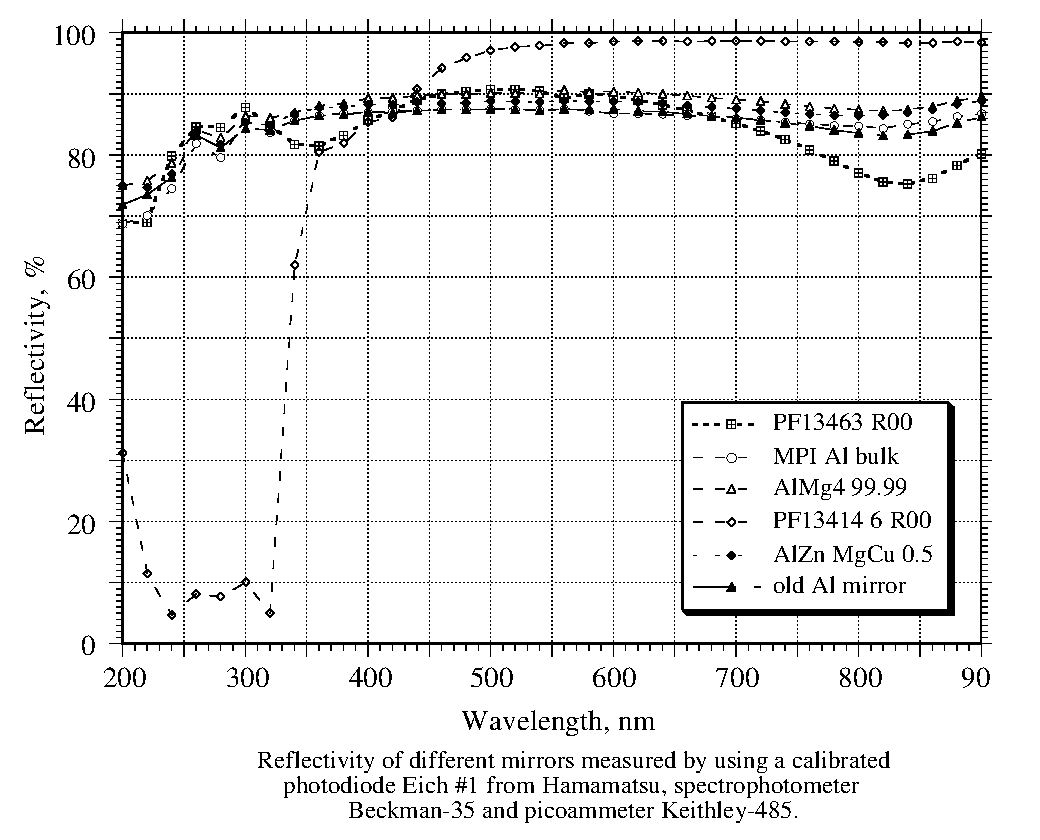
\epsfig{file=bilder/4.2.3.1.eps,height=12cm}
%\end{turn}
%\vspace{-1cm}
\caption{Measured reflectivities for
different types of aluminium and of a silver (PF13414 6 R00) mirrors.}
\label{fig-reflectivity}
\end{center}
\end{figure}

%\FRAME{ftbpFU}{15.0007cm}{11.6992cm}{0pt}{\Qcb{Measured reflectivities for
%different type of aluminium mirrors.}}{\Qlb{fig-reflectivity}}{4.2.3.1.eps}{%
%\special{language "Scientific Word";type "GRAPHIC";maintain-aspect-ratio
%TRUE;display "USEDEF";valid_file "F";width 15.0007cm;height 11.6992cm;depth
%0pt;original-width 484.8125pt;original-height 388.4375pt;cropleft
%"0";croptop "1";cropright "1";cropbottom "0";filename
%'C:/home/docs/magic/prop/bilder/4.2.3.1.eps';file-properties "XNPEU";}}

In
this figure, we also add for comparison the spectral reflectivity of an aluminium
sample overcoated by the company Balzers with Silflex --a reflecting layer of
very pure silver together with a protecting layer-- (see the curve
labeled PF13414 6 R00 in Fig.~\ref{fig-reflectivity}). Silver overcoating would
give about 82\% reflectivity above 370 nm increasing up to
its asymptotic value of $\sim$98\% above 500 nm. 
Because $R$ drops steeply below
360 nm there would be a sizable loss of Cerenkov light excess close to the
zenith angle observations. The conclusion from the reflectivity study is
that diamond machined Al-alloy surfaces do not need an additional pure
aluminium-overcoat for high reflectivity, i.e. one can avoid the costs for
aluminization.

\subsection{Protective mirror overcoating}

\medskip{\it Keyword: The soft aluminium mirror surface needs to be protected by a
hard transparent overcoating}

\medskip

The aluminium mirrors have to be protected by a hard, transparent coating. Three
options are being considered:

\begin{itemize}
\item[(i)]  SiO$_{2}$, vacuum deposited

\item[(ii)]  Al$_{2}$O$_{3}$, grown by anodical oxidation

\item[(iii)]  CVD\footnote{%
CVD stands for Chemical Vapour Deposition} diamond coating
\end{itemize}

The classical coatings are SiO$_{2}$ or Al$_{2}$O$_{3}$. It is only recently
that CVD diamond coating became possible. The technology of SiO$_{2}$
coating is particularly suited for aluminium layers on glass substrates where it is
very important to seal pin holes and the transition edge between the aluminium and the
glass. The technique requires high vacuum and evaporation equipment or
sputtering units. Similarly CVD diamond deposition requires special
equipment and only a few companies are specialized in coating large areas.
Coating with Al$_{2}$O$_{3}$ is the cheapest technique because it can be
carried out in an electrolytic bath under normal lab conditions 
\cite{haas:49,harris:92,loh:93,cresti:96}.
Table \ref{tab-coatings} lists
the main parameters for the different coating materials. It should be noted
that anodization removes some aluminium from the surface and reflectivity is
more affected by deposition of coating material.

\begin{table}[htb]
\centering
\begin{tabular}{|p{1.5in}|p{1.15in}|p{1.15in}|p{1.15in}|}
\hline
Parameter & SiO$_{2}$ & CVD diamond & Al$_{2}$O$_{3}$  \\ 
\hline\hline
Refractive index & 1.45 & 1.5 & 1.6   \\ \hline
Hardness [Mhos] & 6 & 10 & 9   \\ \hline
Production method & Vacuum deposition sputtering & Chemical va\-pour deposition
& Electrolytic oxidation   \\ \hline
Thickness for high &  &  &    \\ 
reflectivity at 400 nm & 100 {\AA } & $\sim$ 100 nm  & 80 {\AA }   \\ \hline
Resistance to wear & Lowest of the 3 & Highest of the 3 & Intermediate   \\ 
\hline
Price/0.25 m$^{2}$ coat. \footnotemark & $\approx 200$ DM & $>500$ DM & $<50$ DM 
 \\ \hline
Drop in $R$ &  &  &    \\ 
by 10\% & $>$ 2.5 years & $\gg$ 10 years & $>$ 2.5 years   \\ \hline
\end{tabular}
\caption{\label{tab-coatings}
 List of parameters of applied coating materials.}
\end{table}
\footnotetext{Large quantities}

The strong argument in favour of CVD diamond coating\footnote{%
Actually, it is not a pure carbon coating but an amorphous Carbon with low
admixtures of hydrogen that has nearly the hardness of diamond but a
refractive index close to 1.5 and an UV transmission down to 250 nm.} is its
excellent resistance to wear, allowing for a lifetime of at least 10 years.
Because of its hardness, the protected surface cannot be damaged by any
abrasive dust during cleaning procedures. The main question is whether the
high cost of this coating can be brought down to acceptable levels in the
next few years.

For MTD96, the electrolytic formation of Al$_2$O$_3$ has been chosen because
of its hardness, its low cost, because it can be done in any laboratory and
because it opens up the possibility of coating the aluminium immediately after
machining. Test have been performed that show that the aluminium alloy has
to be chosen with great care in order to achieve the required reflectivity
of $\geq$ 85\% after coating. Also, ongoing test will show if the coating exhibits the
desired hardness. If this is not so, then an additional vacuum deposit of
pure aluminium will be necessary. Even if this is the case, Al$_2$O$_3$ will still be
chosen since the good properties mentioned above will still hold. The test
results are described in appendix B (``Development of all-aluminium mirrors ...'').

\subsection{Monitoring the mirror reflectivity degradation}

\medskip {\it Keywords: The mirror reflectivity will degrade with time and
monitoring is needed.}

\medskip Here we add a few ideas about monitoring the reflectivity
degradation with time although this chapter would belong more logically to
Chapter 4.4. Monitoring of the telescope's photon to photoelectron
conversion factor is important, for example for energy calibration. One element of
degradation is the mirror reflectivity. Routine checks could be carried out
with a hand-held reflectometer (using a filtered Deuterium lamp spectrum
faking a \Cerenkov spectrum), \cite{bradbury:95}, which turned out to be very
helpful to monitor the reflectivity of the HEGRA telescope mirrors. The main
problem for the MAGIC Telescope is the large number of mirrors to be monitored and the
difficult access. As an alternative we intend to use a deuterium lamp
positioned about a km away from the telescope. The light beam will be
chopped and focused onto the telescope. With the active mirror control (see
next chapter) it will be possible to steer the reflected beam of individual
panels onto a large, broad-band sensitive photocell or Silicon photodiode and
measure the reflected light beam intensity. The intensity can be compared
with a reference mirror and thus degradation can be determined with about
1-2\% precision. The system will be able to scan through all mirror panels
automatically; such a measurement can be carried out within 1-2 hours.

\subsection{The active mirror control}

\medskip {\it Keywords: The mirror support dish deforms under loads and
mirror panels need corrections.}

\medskip The need for an active mirror control has been explained in the
introductory part of Chapter 4.1.1. It has been shown that the requirement
of a rigid mirror support frame and low inertial mass for fast turning
contradict the aim of keeping the cost down. The chosen compromise is a
3-layer space frame with some residual deformation that will require some measure
of active mirror control (which will also very much reduce operator
interference during periodic adjustment). The MAGIC Telescope will be very likely the
first ACT using active mirror control and will thus follow the trend in
large optical telescopes. Nevertheless we would like to point out that the
precision needed in ACTs is about a factor 1000 worse than that in optical
telescopes and a much simpler and cost-effective solution can be used.

The basic principle of the active mirror control is shown in Fig.~\ref{fig-active}.

\begin{figure}[htb]
\begin{center}
%\hspace{-0.5cm}
%\begin{turn}{270}
\epsfig{file=bilder/4.2.5.1.ps,bbllx=0pt,bblly=0pt,bburx=500pt,bbury=800pt,height=12cm}
%\end{turn}
%\vspace{-1cm}
\caption{Schematic view of the active
mirror control system.}
\label{fig-active}
\end{center}
\end{figure}


%\FRAME{ftbpFU}{4.2817in}{5.9957in}{0pt}{\Qcb{Schematic view of the active
%mirror control system.}}{\Qlb{active}}{4.2.5.1.jpg}{\special{language
%"Scientific Word";type "GRAPHIC";maintain-aspect-ratio TRUE;display
%"USEDEF";valid_file "F";width 4.2817in;height 5.9957in;depth
%0pt;original-width 511.6875pt;original-height 718.875pt;cropleft "0";croptop
%"1";cropright "1";cropbottom "0";filename
%'C:/home/docs/magic/prop/bilder/4.2.5.1.jpg';file-properties "XNPEU";}} i

Four
mirror elements will be pre-mounted on a lightweight, rigid support plate
measuring 98 $\times $ 98 cm. Hereinafter this unit will be referred to as a
panel.

The support plate is a commercial sandwich panel consisting of a 20 mm aluminium
HEXCELL core bonded to two 1-mm aluminium sheets of ca. 6 kg m$^{-2}$ total weight.
The 4 mirrors will be pre-adjusted according to their position on the main
dish. In the center of the plate a small laser pointer (685 nm, round beam;
beam divergence 0.35 mrad) will be mounted on a precision jig such that the
light beam can be adjusted to coincide with the focal spot of the 4 mirrors.
The basic unit of ca. 1 m$^2$ will be fixed onto the ca. 1 m$^2$ square grid
of the space frame with 3 adjustment screws that have different degrees of
freedom in their transverse movements. One point is a double high precision
universal joint allowing limited free movements in the $x$-$y $ plane. The
other two incorporate adjustment screws (thread 1 mm/turn) driven by
stepping motors. One of the two motor-driven axes is permanently aligned,
i.e. has no freedom in $x$-$y$, while the other can swivel in one direction.
The stepping motors are driven via a multiplexer by a computer-controlled
drive circuit. Spring preloading of the adjustment screws will minimize the
residual play.

The adjustment proceeds in the following way. The white reflecting camera
cover with some LED markers will be swung in front of the camera.\footnote{%
Alternatively a permanent diffuse reflector panel might be installed beside
the camera. In this case the laser diode spot and focal panel spot will not
coincide but will have to be adjusted such that when the laser is properly
positioned, the mirrors will be focussed onto the center of the camera. This
procedure could in principle be used during normal operation provided no
scattered light of the laser diodes hits the camera or the camera is
insensitive to the used wavelength.} The control computer will switch on the
laser pointer causing the stepping motors of a panel to be adjusted. In
addition, the computer is connected to a CCD video camera with a high power
telelens. This camera, mounted in the center of the mirror dish, will
measure the deviation between the laser diode light spot and the reference
center at the camera cover and drive the stepping motor accordingly until
the laser spot coincides with its reference position. This procedure is then
repeated for all panels one by one. The use of a narrow band pass filter
(matched to the laser emission band) in front of the camera will permit the
adjustment to be carried out even when there is a high level of ambient
background light, thus even during day time. We estimate that it will take
less than 5 seconds for adjusting/checking each panel, i.e. all the panels
could be fine-tuned within 20 minutes. As most mirror panels are not
expected to tilt, the adjustment should be finished in a few minutes. After
some ``training'', the computer should be able to predict the number of
necessary steps with high precision such that no ``hunting'' is expected
during the adjustment or a preadjustment is carried out automatically. This
is particularly important for GRB searches where the telescope must be
repositioned very quickly and no time can be wasted for lengthily adjustment
procedures.

From the finite element analysis of the space frame it is known that the
biggest deformations occur close to the sides where the dish is supported
whereas a large part of the central area shows no deformation at all (see
Fig. \ref{fig-sagging1}). The calculations predict that about 10\% of all panels need
adjustments after a change in declination of 25$^\circ$ and about 25\% after
a change in declination of 60$^\circ$.

We are also considering an alternative procedure that uses as light source
an object at a km distance or a bright star or perhaps the moon. (Although
moonlight is very bright, the moon's image of 0.5$^\circ$ diameter is
difficult to use for adjustments to a precision of $< 0.02^\circ$.) The
panel under adjustment would be tilted so that the panel's focal spot would
be displaced by about 1$^\circ$ out of the general focus. The panel's focus
position would then be recorded by the video camera. The panel would then be
tilted so that the spot moves by ca. 1$^\circ$ to the other side of the
center of the camera. From the two off-axis positions one can interpolate
the correct position and steer the panel accordingly. This procedure is free
of any laser pointer misalignment but cannot be used easily for routine
corrections. Conversely, this procedure allows one to check the laser
alignment and also to check whether the 4 mirrors of a panel are correctly
aligned with respect to each other.

The combination of a tessellated mirror and active mirror control offers
some other benefits. If, accidentally, the telescope points towards the sun
one can defocus the individual elements so that the heat load onto the
camera coverage will be tolerable. It is also possible to check individual
mirror degradation, reflectivity or mechanical defects resulting in focal
degradation, by steering the focal spot of individual panels onto a special
sensor. Most of these operations can be carried out semi (or fully)
automatically from a terminal.

Finally, we want to mention an idea for the initial adjustment of the
mirrors on the telescope. On a cloudy 
late afternoon the telescope will be positioned
such that it points to the zenith. Then, an autocollimating laser plumb-line
will be positioned about 1-2 m above each mirror element. The mirror under
study will be adjusted so that the reflected beam hits the nominal focal
spot on the camera cover. As the volume between camera and mirrors is not
obscured by mechanical elements (masts, steel- or electrical cables). The
plumb-line can be made hanging down on a cable from the camera edge and
pulled across the entire mirror area by 3 transverse strings. The
plumb-line's autocollimation must be able to handle any residual vibration
or oscillation of this rather unstable positioning system. It should be
mentioned that the use of optical plumb-lines for mirror adjustment has been
brought to our attention by F. Krennrich, Whipple collaboration.

Currently we are testing the active mirror alignment on a test stand. The
first tests indicate that a precision equivalent to the video camera pixel
size can be reached (eq. to 2 mm in the focal point). The results of the
first test are both summarized in appendix D (``Test of an active mirror control ...'')
and a diploma thesis \cite{wacker:97}.


\subsection{Protecting the mirrors against environmental impacts}

\medskip {\it Keywords: Protection against environmental impacts has to be
built into the telescope.}

\medskip Since the telescope will not be protected by a dome, it must have
some form of built-in protection, particularly with regard to the mirrors.
There are two classes of environmental damage:

\begin{itemize}
\item[(a)]  impairment of mirror quality during normal operation by dust
deposits or by the formation of dew or ice under conditions of high humidity,

\item[(b)]  rare, but potentially damaging, events such as lightning, storms
or hail.
\end{itemize}

A detailed discussion of the various problems and possible solutions can be
found in chapter 8.2.


\section{The camera}

\medskip {\it Keywords: The \v{C}erenkov light image is detected by a fine
pixelized photomultiplier camera}

\medskip The camera is a decisive element for improving the $\gamma $
sensitivity and the $\gamma $/hadron ($\gamma /$h) separation power.
Historically, ACT cameras underwent a development from a single 
photo multiplier tube (PMT)
version to cameras with a few hundred pixels. The progress of the last years
can mainly be attributed to finer pixelized cameras allowing the subtle
differences between hadron and $\gamma $ showers to be revealed. Hand in
hand with finer pixels there has been an improvement in 
the trigger efficiencies for $\gamma$s, 
the angular resolution,
the $\gamma $/h separation and some modest noise reduction by limiting the
image to its minimal necessary size. In turn also the energy resolution
should be slightly improved
due to the better determination of the shower maximum location
in images, particularly for low energy events. For example
the first HEGRA camera had a pixel size of 0.45$^{\circ }$ although the
typical widths of TeV hadronic and $\gamma $ showers are only 0.2 - 0.4$^{\circ
} $ and 0.1 - 0.2$^{\circ }$, respectively. According to measurement
principles, the pixel size should be $\leq $ 1/2 of the quantity to be
measured, i.e. as ``width'' is a good discrimination parameter, the pixel
size should be $\leq 0.1^{\circ }$. A similar pixel size can be derived from
the needed angular resolution and the other image parameters. Here we would
like to reiterate that distant showers (high up in the atmosphere or at
large zenith angles) will produce more compressed images that demand finer
pixels. On the other hand fine granularity is very costly, with regard to
both the sensor and the associated readout. Eventually the investment for
the camera and readout electronics will dominate the cost of the telescope;
compromises have to be found.

Besides the pixel size, image analysis is also affected by the diameter of
the camera. The shower image can easily extend up to one degree (1.5-2$%
^\circ $ for energetic showers) and it is very important to also collect
information about the shower tail (being farthest away from the camera
centre) for $\gamma$/h separation and for solving the head/tail ambiguity
of images.

As has already been pointed out, images from distant, low energy showers
($<$ 100 GeV)
will be rather compressed and rather close to the camera centre while high
energy showers with plenty of light will be more extended because they reach
further down into the atmosphere. This influences the configuration and size
of the camera. For cost reasons the following compromise for the MTD96
camera has been reached. The inner part of the camera will be equipped with
high QE, red-extended pixels 0.1$^\circ$ in size up to a radius of 
1.25$^\circ$. The high resolution section will be surrounded by coarser pixels
0.2$^\circ$ in size and normal bialkali photocathodes. The ``low QE'' ring
extends from 1.25$^\circ$ 
up to 1.8$^\circ$ radius  and is sufficient for the observation of
the tails of
high energy showers where plenty of light is generated anyhow. Fig.~\ref{fig-pattern} 
shows the geometrical pixel pattern.
\begin{figure}[htb]
%\hspace{-0.5cm}
%\begin{turn}{270}
\leavevmode
\centering
\epsfxsize=12cm
\epsffile{bilder/magic-camera.eps}
%\end{turn}
%\vspace{-1cm}
\caption{Geometrical pixel pattern of 
a possible design of the MAGIC Telescope's
camera.}
\vspace{1pc}
\label{fig-pattern}
\end{figure}

This `mixed' camera can be considered as a staged version of an `all high
QE' fine pixel camera which might eventually be needed for the study of
extended sources. Eventually we will aim for a 4 - 5$^\circ$ {\o} field-of-view camera with
nearly round geometry.

Before describing the camera in detail we would like to elaborate more on
the benefits of using red extended, high QE sensors, although they are
considerably more expensive than conventional PMTs, the ``workhorse'' of all
contemporary ACTs.

The classical PMTs with bialkali photocathode and borosilicate windows are
well suited for the observation of \v{C}erenkov light from showers in the TeV
region. The spectral cut-off of standard glass windows is reasonably matched to
the Ozone cut-off of the atmosphere while the QE peaking between 300 and 450
nm is well matched with the UV peaking of the \v{C}erenkov light. In addition
the contribution of the night sky background in the UV is rather low. The
situation changes quite significantly when distant showers are observed,
e.g.\ when observing at large zenith angles or when observing low energy
showers that stop high up in the atmosphere. Rayleigh and Mie scattering
will scatter most of the short wave \v{C}erenkov photons in such a way that the
remaining spectrum at the detector level shifts peaks to higher wavelengths.
For example, at a zenith angle of 75$^\circ$ the spectrum is rather flat
between 400 and 600 nm with its peak around 450 nm, whereas below 350 nm
almost no light at all is observed. 
An independent confirmation of the
effect can be derived from measurements of the solar spectrum at different
air masses, see for example Fig.~\ref{fig:3.3}. The low energy showers, 
which are most
difficult to observe, peak at around $x_{{\rm max}} \approx 0.2$ air mass,
i.e., besides a small absorption correction due to high layers of Ozone
the curves in chapter~3.7 should fairly well represent the
reduction due to scattering and absorption processes in the atmosphere.

A closer look at the night-sky background shows that one would still gain in
the value of $S/\sqrt{NSB}$ by extending the sensitivity towards the `red'
because $S/\sqrt{NSB}$ increases more slowly than $S$ as a function of
wavelength. 
Here we wish to mention that for an imaging telescope it is not only
the $S/\sqrt{NSB}$ ratio is important, but also the absolute number of
ph.e.s measured per image. Obviously, by extending the measurement of the
\Cerenkov spectrum further into the red, one collects more charge. 
We would like to point out that some subtle effects, such as the
excess noise of PMTs or the electronics system noise, encourage one to work
with the largest possible value of $S$ even if $S/\sqrt{NSB}$ increases
proportionally.

Another strong argument in favour of using red-extended light sensors comes
from the prospect of carrying out observations in the presence of moonlight.
Unless one is observing within a few degrees around the moon, one is
confronted only with a background of scattered moonlight. Direct moonlight
exhibits a very similar spectrum to that of the sun. Scattered moonlight is
``blue''; the blue sky on a clear day is an example of this. Depending on
the telescope's altitude and the moon's zenith angle, scattered moonlight
will show peaks around 400 nm with nearly half of its photons below this
wavelength. Fig.~\ref{fig:3.6} shows sample spectra for scattered sunlight with
aerosol concentration as an additional parameter. From the curve with low
aerosol concentration which corresponds $\approx$ to a clear sky condition
at the HEGRA site
it is immediately obvious that it would be favourable
to integrate the \v{C}erenkov light up to $\sim $ 600 nm. Some relevant values
for the moonlight are:

\begin{center}
\begin{tabular}{l@{\hspace{0.3cm}}l}
Direct photon flux (full moon): & ca. 2.10$^{14}$ photons m$^{-2}$ s$^{-1}$
\\ 
scattered photon flux (full moon): & ca. $10^{13}$ photons m$^{-2}$
sterad$^{-1}$ s$^{-1}$%
\end{tabular}
\end{center}

A critical background factor during observations in presence of moonlight is
the light that is scattered off the nearby ground or reflected from parts of
the telescope. Great care will have to be taken to avoid scattering from the
telescope structure and to minimize the angular acceptance of the Winston
cones in front of the sensors for light outside the angular range defined by
the mirror area.

The improvement achieved by using a high QE red-sensitive photosensor
instead of classical PMTs for observations at large zenith angles should be
very high, e.g.\ a factor ca. 4.5 at 70$^\circ$ for 50 GeV showers. For
silicon avalanche photo diodes (APDs)
the gain can reach easily a factor 10 (see Section 4.3.3).

The prime focus detector package (including the camera, HV generators,
pre-amps, optical fiber drivers and housing) will weigh about 100-120 kg. To
keep the shadowing of the reflector to a minimum, the external dimensions of
the housing of the MTD 96 design will not exceed 125 $\times$ 125 $\times $
100 cm, allowing a maximal camera diameter of 4$^\circ$. Various camera
designs are considered (see below). Each will be modular to permit easy
exchange of parts, and the option of generating solar power via a prime
focus heat exchanger will be retained. The detector package could be
circular to allow for rotation; in this case the package will be equipped
with stepping motors that allow rotation up to 180$^\circ$, thus maintaining
the orientation of the star field in the camera co-ordinate system
throughout the course of each observation, a feature of particular
importance for the study of extended objects (see discussion below).

The sensitive area of the MTD96 camera has a diameter of 3.6$^{\circ }$ in
the focal plane (equivalent to a diameter of approx. 100 cm) and consists of
a fine pixelization region 2.5$^{\circ }$ in area surrounded by a few rings
with coarser pixels that are naturally inferior in performance but lower in
price. Triggers will be derived from part of the inner section which has a
diameter of 1.6$^{\circ }$.

In the following section we will describe details of the camera. Three
versions are discussed. The MTD96 camera is a mixture of high QE, red
extended hybrid PMTs (commonly called hybrid photo detectors (HPDs)) 
in the central part and a ring of
conventional bialkali PMTs. If, for unexpected reasons, the novel hybrid PMTs
are not available, we will resort to using a conventional PMT camera. Also we
wish to discuss the option of building a camera with APDs as light sensors.
These detectors with ca. 80\% QE have not yet the required low-noise
performance but it is hoped that within a few years this will be possible.
An APD equipped 17-m telescope will correspond to a ``classical'' telescope
of over 45 m diameter.

%\vfill

\subsection{The MTD96 camera based on high QE GaAsP - intensified photocells
with avalanche diode readout}

\medskip {\it Keywords: The Intevac GaAsP-intensified photocell as a parent
type for a \v{C}erenkov photosensor.}

\medskip We intend to use vacuum photosensors with a GaAsP photocathode
because the cathode offers a broader and superior QE compared to bialkali
PMTs. The company Intevac offers a commercial photosensor with an 8 (16) mm 
{\o} GaAsP photocathode. This rather compact detector is a HPD 
(called intensified photocell (IPC) by Intevac) with a 1 mm {\o} GaAs
PIN diode as anode. Photoelectrons are accelerated by a cathode to an anode
voltage of 2-10 kV$_{{\rm c-a}}$ and generate up to about 1500 electron-hole
pairs in the diode. Fig.~\ref{fig-hybrid_tube} shows a cross-section of 
a tube with a 16 mm {\o} cathode 
and Fig.~\ref{fig-spectral} the spectral curve (plain tube labeled
as 'Intevac-clean') of a sample
tube when cross-calibrated against a reference silicon photodiode.

\begin{figure}[htb]
%\hspace{-0.5cm}
%\begin{turn}{270}
\leavevmode
\centering
\epsfxsize=10cm
\epsffile{bilder/4.3.1.1.ps}
%\epsfig{file=bilder/4.3.1.1.ps,bbllx=0pt,bblly=0pt,bburx=500pt,bbury=800pt,width=11cm}
%\end{turn}
%\vspace{-1cm}
\caption{Cross section of a hybrid
photomultiplier with avalanche diode readout.}
\label{fig-hybrid_tube}
\end{figure}

Some
modifications are necessary in order to adapt the device for the proposed
use:

\begin{itemize}
\item[a)]  The QE below 400 nm is too low, i.e.\ below that of bialkali
photocathodes (the curve labeled 'PMT EMI-9083 A'
in Fig.~\ref{fig-spectral}). A solution to enhance the UV sensitivity with wavelength
shifters (WLS) will be discussed in the next section.

\item[b)]  The gain of the IPC is too low to achieve single electron
response in the ns time domain. The output signal has to be amplified by a
transimpedance amplifier or a very fast charge sensitive amplifier to a few
mV per ph.e. Even the best fast amplifiers have an equivalent input noise
charge of a few thousand electrons in the 1-10 ns time domain. The solution
is to replace the diode by an avalanche diode giving additional gain. This
development will be discussed in Section 4.3.1. The first prototype tubes
have been tested.
\end{itemize}

As noted in the overview of the camera, the MTD96 will be equipped with IPCs
up to a radius of 1.25$^{\circ }$ only, whereas we intend to increase the
radius to 1.8$^{\circ }$ by adding rings of conventional bialkali PMTs. These
are the same as in the classical version, the so-called `fallback' option,
and a detailed description can be found in Section 4.3.2. Fig.~\ref{fig-block}
shows a basic block diagram of a single pixel.

The elements are
\begin{itemize}
\item  a hollow Winston cone light funnel,

\item  a hybrid photomultiplier with a GaAsP high QE, red-extended
photocathode and WLS coating for UV extension,

\item  a high-voltage power supply for $U_{\mathrm{c{\rm -a}}}$,

\item  a high-stability, medium-voltage supply for the AD bias,

\item  an AC-coupled preamplifier (transimpedance or charge sensitive)
followed by a filter amplifier followed by the driver for the analog optical
fiber ,

\item  possibly a parallel slow branch measuring the mean current output of
the IPC as a coarse measure of the night sky background.
\end{itemize}
Obtained studies of some tubes are added in the appendix E.

\begin{figure}[htb]
\begin{center}
%\hspace{-0.5cm}
%\begin{turn}{270}
\epsfig{file=bilder/4.3.1.2.eps,width=15cm}
%\end{turn}
%\vspace{-1cm}
\caption{Spectral Quantum Efficiency of
an Intevac hybrid PMT compared to a classical bialkali-PMT, an APD, and an
Intevac tube covered by a wavelength shifter dye to enhance the efficiency
in the blue. The APD curve is taken from \cite{pansart:97}.}
\label{fig-spectral}
\end{center}
\end{figure}


\begin{figure}[htb]
\begin{center}
\epsfig{file=bilder/4.3.1.1.1.eps,width=15cm}
\caption{Basic block diagram of a
single camera pixel readout chain.}
\label{fig-block}
\end{center}
\end{figure} 
\vspace*{1cm}

\clearpage
\newpage
\subsubsection{Enhancing the UV sensitivity by WLS coating of the window}

\medskip {\it Keywords: The low UV sensitivity of the Intevac tubes can be
enhanced by a simple WLS coating.}

\medskip In order to make full use of the \v{C}erenkov spectrum reaching the
telescope the UV sensitivity of the IPC has to be enhanced. A
straightforward and simple procedure is to coat the window with a WLS that
shifts the UV light to the wavelength at which the IPC shows maximum
sensitivity. The WLS method has been in use for many years in high energy
physics \v{C}erenkov detectors where it offers a simple remedy for the UV
cut-off of the PMT glass windows. Fluorescent dyes, particularly those used
for dye lasers, are well suited for this purpose because many of them have
a QE close to 100\% and decay times in the ns range. These dyes can either
be evaporated directly onto the window or embedded in a plastic carrier. The
latter method is more efficient because of better light trapping, ease of
application (as a foil or lacquer) and much higher mechanical resistance.
Examples for the lacquer coating of PMT windows can be found in Eigen et al.
(1979) and Bradbury et al. (1995). For example, all the PMTs of the HEGRA
AIROBICC detector are coated with WLS in order to improve the UV-sensitivity
between 300 and 330 nm. Some suitable dyes for our application are
P-terphenyl, Butyl-PBD, POPOP, PMP, and modified Perylene (BASF dye \# 078
or 241), etc. The dyes can be dissolved together with a polystyrene or
Paraloid (an acrylic lacquer base) binder in organic solvents such as
dioxan, chloroform, toluol or dichloromethane and applied as lacquer or thin
foil to the window. The window can be overcoated a second time by a thin
layer (a few $\mu $m) of Teflon AF, which acts as a simple antireflex
coating because of its low refractive index ($n$ = 1.3). Tests of WLS
coating on the IPC showed a clear increase in UV-sensitivity; see example
in Fig.~\ref{fig-spectral}
(the curve labeled as 'Intevac + WLS'). 
However, the gain did not reach the predicted value of
around 40\% because the current window geometry is not ideal for WLS light
collection. For strength reasons, a tapered glass window of 5.6 mm thickness
(see Fig.~\ref{fig-hybrid_tube}), was used in the commercial tube. The WLS emits light
isotropically. Besides the inevitable loss of ca.\ 12.7\% in the backward
direction, all the light is normally trapped in the high-refractive index
glass and has thus a high probability of hitting the photocathode. In the
case of the tapered 5.6 mm window of the IPDs, about 45\% of the light
misses the cathode. This deficiency can be corrected by using a light-fiber
plate or a thin, high-strength artificial sapphire window. Light-fiber
plates have other losses and are therefore less suitable. We have tested 1
mm thick sapphire windows at up to 30 atm without breaking them. Sapphire is
used in ultra high vacuum applications at up to 10$^{-10}$ Torr and is
easily available because of its widespread use in wrist-watch windows. Its
thermal expansion coefficient of ca. $6\cdot 10^{-5}$ is closely matched to
Kovar, as well to the ceramic material of the tube body and to GaAs. Its
high melting point prevents melt bonding of the GaAsP wafer cathode directly
onto the window but so-called solder glasses of matched expansion
coefficient and a softening temperature of ca. 350$^{\circ }$C can be found
readily. Because it has a higher refractive index than glass plain sapphire
will have higher reflective losses than glass but, with the surface coating.
of the plastic WLS carrier and Teflon AF, the losses can be reduced to $<3\%$.
The window is normally fixed to the tube body by an indium seal. Our tests
confirmed that a 
uniformly distributed load of $\mathrm{>}$ 1500 kg can be applied without
breaking an artificial sapphire window, 22 mm in diameter and 1 mm thick. In
summary, we are confident that one can achieve a QE $>40\%$ from 300 to
nearly 650 nm with the modified IPC. Because of the WLS decay time a small
degradation of the time resolution will occur but it will still be below the
1-2 ns time spread of the \v{C}erenkov light.

\subsubsection{The increase of the IPC gain}

\medskip {\it Keywords: The gain of the commercial IPCs is insufficient to
resolve single electrons on a few ns time base.}

\medskip The gain of ca.\ 1000 of the parent type IPC is too low for a good
single electron response in the ns time domain. Recently Intevac has
replaced in a prototype IPC the GaAs PIN diode by a GaAs Schottky avalanche
diode (AD). At a bias of ca. 30 V the AD has an internal gain of 10-15
resulting in an overall device gain of ca. 25,000 at 10 kV$_{{\rm c-a}}$.
GaAs allows for a very high operating frequency (up to 4 GHz in the IPC). As
we have less demanding speed conditions we intend to replace the GaAs AD by
a silicon one for the following reasons: we are interested in running the
tube in rather harsh field environments and want to lower the $U_{{\rm c-a}}$
to $< 5$ kV, thus the primary gain would be reduced. This reduction has to
be compensated for by a higher AD gain. In addition we plan to raise the
overall gain to about {\mbox30,000}-{\mbox50,000} because it allows for cheaper and less
complex transimpedance amplifiers
or maybe even current amplifiers. A high gain in a GaAs-AD cannot be
achieved because of the nearly equal k-factors of hole and electron
multiplication. Silicon ADs are now well under control up to gains of, say,
200. Also the energy required to create an electron-hole pair in silicon is
lower than in GaAs (3.6 eV vs. 4.2 eV) thus the silicon AD will have a
higher multiplication for the same $U_{{\rm c-a}}$. In addition, the lower $Z$
of silicon compared to GaAs will result in less back scatter and hence give
an intrinsically better single electron resolution\footnote{In principle
such an excellent electron resolution is not needed but improves slightly
the background rejection ('tail cuts') and errors on the individual pixel content.
Nevertheless one has to consider that for very short shaping times the resolution deteriorates
proportional to 1/$sqrt{\tau}$, $\tau$ being the shaping time constant. In case of
aberrations in the presence of moon light it is unnecessary to resolve
single electrons because the background light noise is much larger than a single
electron.}.

We have tested the single electron response of the prototype IPC using a
blue LED light pulser of 5 ns FWHM and $\langle n_{{\rm photon}}\rangle
\approx $ 6-8. 
%Fig.~\ref{fig-block} shows the basic block diagram of the test
%set-up and 
Fig.~\ref{fig-phe} shows the resulting pulse height distributions for
10 kV$_{{\rm c-a}}$ and a 50 ns filter time constant. The peaks for 1,2,3..
electrons are well resolved.

\begin{figure}[htb]
\begin{center}
%\hspace{-0.5cm}
\begin{turn}{270}
\epsfig{file=bilder/spectral.ps,bbllx=0pt,bblly=0pt,bburx=500pt,bbury=800pt,height=12cm}
\end{turn}
\vspace{1cm}
\caption{Pulse height spectrum of a
modified Intevac IPC when illuminated by a fast blue LED pulser. Settings: $%
U_{{\rm c-a}}=\ 10$ kV; $U_{{\rm AP}}=\ 30.0$ V, $\tau =\ 50$ ns.}
\label{fig-phe}
\end{center}
\end{figure}

%\FRAME{ftbpFU}{5.0963in}{3.5103in}{0pt}{\Qcb{Pulse height spectrum of a
%modified Intevac IPC when illuminated by a fast blue LED pulser. Settings: $%
%U_{{\rm c-a}}=\ 10$ kV; $U_{{\rm AP}}=\ 30.0$ V, $\tau =\ 50$ ns. }}{\Qlb{%
%fig-phe}}{spectral.jpg}{\special{language "Scientific Word";type
%"GRAPHIC";maintain-aspect-ratio TRUE;display "USEDEF";valid_file "F";width
%5.0963in;height 3.5103in;depth 0pt;original-width 212.875pt;original-height
%146.0625pt;cropleft "0";croptop "1";cropright "1";cropbottom "0";filename
%'C:/home/docs/magic/prop/bilder/spectral.jpg';file-properties "XNPEU";}}

We also tested a second set of operational parameters:
With 6 kV$_{{\rm c-a}}$ and a 10 ns filter time constant (i.e.
settings much closer to our final operating conditions) the electron peaks
are still distinguishable but much wider. The pulse height resolution
would in principle be just acceptable for us but
in a large system one would want to have better performance to counteract
degradation due to component spreads and time. The use of a silicon AD of
1.5 mm {\o} and of gain 30-60 seems to be the best solution.

\subsubsection{The ion feedback problem}

\medskip {\it Keywords: Ions in PMTs can fake large signals and destroy the
photocathode}

\medskip In our application the photosensor will work in a high background
environment. The large mirror will collect a high flux of the night sky
background light (ca. $1.7 \cdot 10^{12}$ photons m$^{-2}$ sterad$^{-1}$ s$%
^{-1}$ between 300 and 600 nm) resulting in a single photoelectron counting
rate in excess of 50 MHz per pixel. While the probability of ionizing the rest gas
between cathode and anode is low because of a vacuum of 10$^{-8}$ Torr, the
rate of ionization of the rest-gas adsorbed on the AD surface and
surrounding metal layer will generate a sizable flow of ions. This
back-flow (presumably mostly hydrogen ions) will have two adverse effects on
the photocathode: (a) it will frequently generate large pulses that can fake
large \v{C}erenkov signals \cite{mirzoyan:94} and (b) it will 
eventually destroy the
activation of the photocathode\footnote{According to Intevac a drop in 
cathode sensitivity by a factor of 2 will occur after an integrated current
of 5 mC. This can be coverted into $<$ 100 years of dark night
observations, or 10-15 years of observations both during
dark nights and during moonlight.}

The ions can be deflected electrostatically such that they miss the
photocathode. 
\begin{figure}[htb]
\begin{center}
%\hspace{-0.5cm}
\epsfig{file=bilder/intevac1.ps,height=6cm}
\epsfig{file=bilder/intevac2.ps,height=6cm}
\vspace{1cm}
\caption{Simulation of of a) electron tracks, and b) ion tracks
inside the Intevac IPC employing an electrostatic deflector.}
\label{fig-intevac_simul}
\end{center}
\end{figure}

Fig.~\ref{fig-intevac_simul} 
shows a simulation of a) electron tracks, and b) ion tracks
inside the Intevac IPC. The simulation
was carried out by Intevac using their patented 
electrostatic deflector, a small conductive
finger at ground potential. The small deflection of the higher energy
electrons is compensated for by a small offset of the AD from the center. A
test of the prototype IPC with an 8-mm GaAsP photocathode gave a noise rate
of ca. 10 kHz but a very low rate of large signals that are compatible with
the rate of \v{C}erenkov signals of cosmic muons passing through the thick glass
window.

The Zagreb group has made detailed electron optics simulation and found a
configuration that allows to completely suppress the ion feedback from the
anode area while conserving the rotational symmetry. The proposed special
electrostatic `lens' could be used also in classical PMTs and help to reduce
the ion feedback problems in case of high ambient background illumination.
The results of the study are summarized in appendix F (``Electron optics
of the Intevac intensified photo cell).

\subsubsection{Comments/conclusions on the IPCs and the studies}

\medskip {\it Keywords: GaAsP photosensors allow for a factor 3-5 increase
in photon to photoelectron conversion}

\medskip The use of high QE, red-extended photosensors is of great
importance for HE $\gamma$-astronomy with ACTs. For the time being they are
`on the critical path' of MAGIC. The current prototype work shows that they
can be built and that the problem lies more in the commercialization of the
design. The current studies show that

\begin{itemize}
\item[(a)]  an acceptable UV extension of the spectral sensitivity can be
obtained for GaAsP photocathodes by applying a WLS coating to thin windows;

\item[(b)]  that artificial sapphire, 1 mm thick, is a good window candidate
because of its high strength;

\item[(c)]  that the replacement of the anode diode by an 
avalanche diode allows for
sufficient gain to be able to have a good single electron response at very
high rates;

\item[(d)]  the high vacuum and proposed electron optics with an ion
deflector (current version or simulated new electron optics configuration)
prevent destruction of the cathode activation by ion feedback and keeps the
rate of large fake pulses low.
\end{itemize}

In appendix E we show the results of a recent study with an Intevac prototype.

All the tests carried out so far indicate that the use of such a
photosensor will increase the conversion yield of \v{C}erenkov light to ph.e.s by a
factor of about 4 over conventional bialkali PMTs when observing close to the
zenith and a factor of about 5 at low altitude (ca. 15$^\circ$)
observations, i.e. the use of such a tube compares to the construction of an
ACT of 30-40 m {\o} mirror and classical PMTs.

The production of the tube is rather complex and therefore more expensive
than the production of glass PMTs with in situ formation of multialkali
cathodes. The cathode has to be grown by Epitaxy onto a thin GaAs waver,
then it has to be fused onto the glass (sapphire) window. Afterwards the
GaAs has to be etched away. In a next step the cathode has to be coated with
Caesium or Ceasiumoxyde in order to lower the escape barrier. Finally the
window has to be mated with the other parts of the tube. Nearly all steps
have to be done under ultrahigh vacuum. It is obvious that this production
requires the collaboration of people experienced in semiconductor production
and in ordinary PMT production. GaAsP photocathodes are used as
electron sources in electron accelerators and as photocathodes in the latest
generation of image intensifiers (night-vision units). Therefore the
principle of the photocathode production is fairly well known. Recently we
have begun discussions with a Japanese and an European PMT manufacturer about
possible production of the hybrid PMTs with GaAsP photocathodes. In parallel
we are discussing the direct epitaxial growth of GaAsP photocathodes on
sapphire with some Russian companies.

It should be noted that the recent measurement with the IPC with AD readout
\cite{beaune:96} is somehow a `world best' measurement of low photon flux
detection with fast timing. Such devices could have many other applications
such as for example fast fluorescence studies of biological processes, low
light detection in astronomical observations of pulsars or high resolution 
$\gamma$ spectroscopy using CsI(Tl) crystal detectors or scintillators of very low
light yield and long wavelength emission.

%Figure captions Fig.~4.3.1/1 Comparison of the QE of various photocathodes
%(original ref. unknown)
%
%Fig. 4.3.1/2 Cross section of the commercial Intevac IPC
%
%Fig. 4.3.1.2/1 Measured spectral sensitivity of an INTEVAC IPC without and
%with WLS coatings
%
%Fig. 4.3.1.3/1 Block diagram for a test of the modified Intevac IPC with
%avalanche diode readout.
%
%Fig. 4.3.1.3/2 Pulse height spectrum of a modified Intevac IPC when
%illuminated by a fast blue LED pulser. (a) $U_{{\rm c-a}}=\ 6$ kV; $U_{{\rm %
%AP}}=\ 30.0$ V, $\tau =\ 10$ ns. (b) $U_{{\rm c-a}}$ = 10 kV; $\tau =\ 50$
%ns.
%
%Fig. 4.3.1.4 Calculation of photoelectron and ion traces in the modified
%IPC. Calculation by Intevac.

\subsubsection{The light funnels in front of the light sensors}

\medskip {\it Keywords: Hollow Winston cones are used for $\approx$ 100\%
light collection and suppression of large angle stray light}

\medskip For constructions reasons, light sensors, classical PMTs or hybrid
PMTs (or APDs) have a sensitive area significantly smaller than their outer
dimensions. Therefore, even in a physically very dense package, a sizable
fraction (ca. 50\%) of the light would be wasted. A way out is to install
light funnels, which are now in use in many telescopes (for example at CAT
or HEGRA). A careful design would result in nearly 100\% light collection.
In MAGIC we will use hexagonal to round (29 mm to 15 mm {\o}) hollow
light funnels shaped like Winston cones. In principle, the funnels allow for
an area compression of 4.5 by reducing the angular acceptance to 0.8 sterad.
This reduction is of great importance as it limits the angular acceptance
corresponding to an area slightly larger than the mirror area. Therefore the
camera would be insensitive to stray light from angles $>$ 33$^\circ$, i.e.
from back-scattered light from the ground, for example during moonshine or
distant light from human installations, cars, snow in winter, etc. Only a
small extra baffle around the camera might be needed in order to minimize
double-scattered photons.

The cones would be made similar to those in use in the current HEGRA
telescopes. Delrin mandrels resembling the shape of the cones will be
mounted, densely packed, onto a transfer plate and the gap between the
mandrels will be filled with black microsphere-filled Epoxy. After hardening
the mandrels can be removed and, after some machining of excess material,
the slightly oversized cones, made from high quality aluminized Mylar, will
be glued in. The dead space between the cones is just twice the thickness of
the 0.1 mm Mylar.

The change from hexagonal to round can be accommodated by proper folding of
the Mylar with only a modest deviation from an ideal Winston cone shape
(rotation of an inclined parabola). This technique has been developed at the
MPI in Munich and has been in use on 5 of the 6 HEGRA telescopes.
Fig.~\ref{fig-winston} shows a photo of a HEGRA light funnel plate for 271 pixels.

\begin{figure}[htb]
\begin{center}
%\hspace{-0.5cm}
\begin{turn}{270}
\epsfig{file=bilder/4.3.1.6_1.PS,bbllx=0pt,bblly=0pt,bburx=500pt,bbury=800pt,height=14cm}
\end{turn}
\vspace{1cm}
\caption{Photograph of the hollow light
funnel (Winston cone) plate for the HEGRA ACTs.}
\label{fig-winston}
\end{center}
\end{figure}

In front of the light funnels a thin window will be mounted. Its main
function is to hermetically seal the electronic sensors and elements against
humidity and dust. The window will have a high transmission between 300 and
700 nm. In order to minimize light losses by surface reflection we intend to
use either a 1 mm TEFLON AF window (lower wavelength spectral cut-off around
210 nm; $n$ = 1.3, i.e., a reflectivity loss of about 3.4\%) or a 1 mm
Plexiglas 218 plate with antireflex coating (lower spectral wavelength
cut-off $\approx $ 290 nm).

\subsubsection{The HT system for the IPCs}

\medskip {\it Keywords: The IPCs need 5-8 kV bias voltage.}

\medskip The IPCs need between 2.5 and 8 kV between photocathode and anode.
We intend to operate the tubes at a nominal value of 5 kV, but, because of
device spreads and ageing, a variation between 3 and 8 kV must be allowed.
At 5 kV the bleeder network across the tube draws about 1 $\mu$A of current.
We will use Greinacher voltage multipliers that are able to supply 180 $\mu$%
A at 8 kV, e.g. we will always connect 50 IPCs together to one supply. A
series potentiometer in front of each IPC allows for some equalibration of
the gains in each batch. This equalization will be carried out beforehand on
a lab bench. The voltage of each batch will be controlled by the on-line
system via DACs.

Most of the HT system will be potted in order to avoid corona discharge.
Also, it will be important to seal the camera and flush the interior by dry
nitrogen or SF$_6$ (with some modest overpressure) in order to prevent humid
air to enter the camera.

For the more technically interested reader: the first step gain due to the
electron bombarding of the silicon anode(PIN diode or AD) is: 
\[
\begin{array}{lll}
G_{\mathrm{bias}} & \approx & (U_{{\rm bias}}-2500\ {\rm V})/3.67\ {\rm eV} \\ 
&  & \mathrm{with \, G = gain} \\ 
U_{{\rm bias}} & = & \mathrm{bias \, voltage \, of \, the \, IPC \, in \, V} \\ 
2500\mathrm{V} & = & \mathrm{min. \, voltage \, needed \, to \, pass \, the \,
passivation \, and \, p++ \, layer \, of \, the \, diode} \\ 
3.67\mathrm{eV} & = & \mathrm{energy \, needed \, to \, create \, an \, electron-hole \, pair}
\end{array}
\]
At around 6.2 kV the gain is ca. 1000. Due to the linear correlation of the
gain and bias voltage the gradient $\Delta G/\Delta U$ is basically constant
and very small. Therefore the requirements for bias-stability are less
stringent than for classical PMTs.

\subsubsection{The bias voltage for the avalanche diodes}

\medskip {\it Keywords: the ADs need a highly regulated bias voltage around
50-100 V.}

\medskip The ADs inside the IPCs need a highly stabilized bias voltage,
which has to be generated for each AD separately. We plan to use a common
bias rail of $-150$ V, a 100 k$\Omega$ pre-bias resistor and a parallel load to the
AD (see Fig.~\ref{fig-block}). The parallel load is driven by a reference signal
(computer-controlled DAC), a temperature sensor and the actual voltage at
the AD load resistor. The voltage at the network and the AD are measured
automatically and used to record the gain and the AD current which is to a
certain extent a measure of the background light. The parallel load
regulator ensures automatic protection against destructive AD overloads in
the case of high-light levels.

The gain of the AD will be set to ca. 30-50, i.e. the IPC will have an
overall gain of 30,000 - 50,000.

%Fig. 4.3.1.7/1 Block diagram of the bias network of the AD inside the IPC.

\subsubsection{The fast preamplifier and filter amplifier}

\medskip {\it Keywords: The IPC's low output signal needs to be amplified}

\medskip The electrical signal of 30,000-50,000 electrons per
incident photoelectron is still too small to be handled by standard fast-electronic
components and needs to be amplified by a large factor. Most suitable are
either low noise charge sensitive preamplifiers followed by filter
amplifiers of appropriate filter time constants in the 5 ns range or
ultralow noise transimpedance preamplifiers. In both cases the preamplifier
must have an intrinsic noise well below 30,000 electrons in the needed
frequency band. Prototypes of either type of preamplifier have been built
and found to be acceptable in noise performance but the safety margins are
not large and some improvements are needed. Due to the rapid expansion of
the mobile phone system in the 900 MHz band, new low-noise, cheap microwave
transistors, suitable also for our application, are becoming available now.
The filter amplifiers are fairly standard items. Therefore we will not
discuss them any further. In the case of the transimpedance amplifier the
filter amplifier will be a simple high bandwidth voltage amplifier with some
modest integration and differentiation.

\subsubsection{The outer ring of classical PMTs in the camera}

\medskip {\it Keywords : For cost reasons the outer ring of the camera will
be equipped with classical PMTs of larger diameter}

\medskip For cost reasons, we plan to use classical PMTs of 0.2$^{\circ }$
pixel size in the outer section of the camera. Images of the most
interesting $\gamma $s , i.e.\ in the energy domain below, say, 200 GeV or at
large zenith angles, hardly extend to outside the inner 1.25$^{\circ }$ radius of
the camera. On the other hand, shower images of TeV $\gamma $s produce a
sufficient amount of light so that classical PMTs would detect them, provided
the camera is large enough (ca. 2500 photoelectrons/TeV $\gamma $ energy in
a classical PMT camera). In the outer ring one records mostly the photons of
the shower tail. Due to the natural spread of the shower tail the
corresponding section of the image is rather diffuse and a coarse pixel size
of 0.2$^{\circ }$ is sufficient. We intend to use 2'' PMTs
which can be retrieved from a large sample of PMTs left over from high energy
physics experiments. The PMTs will be operated also at a gain of 
\mbox{30,000} - \mbox{50,000}
(only 6-8 stages used) and followed by the preamplifier-filter amplifier chain as
outlined in the preceding section.

Further information on the standard PMTs can be found in the following
sections. It should be mentioned that we consider the use of an outer ring
of classical PMTs also as a staged approach to eventually build a
large-diameter camera with uniform, fine pixel size of high QE PMTs. The
needs and time scale is very likely dictated by the existence, or
non-existence, of extended $\gamma $-sources. In the former case the use for
a large diameter, uniform camera is important.

\subsection{The classical camera version}

\medskip {\it Keywords: As fallback solution in case of development delays
or staging a classical PMT is used as interim solution}

\medskip The plan to use a new type of photon detectors is quite ambitious,
and for various reasons it might be necessary to invest more time into their
development; or, for financial reasons it might be necessary to stage the
construction. As outlined in the introduction, one can use the so-called
fallback solution by building a classical PMT camera. This will influence
the potential of MAGIC as the trigger threshold will rise from about
10 GeV to about 30 GeV in the zenith position. This is still significantly
better than for any currently proposed project but the chances to carry out
large zenith angle observations will be affected. Detailed comparisons
of the performance are made in chapter \ref{chap-6}. A possible scenario
could be that one builds the telescope as soon as possible and uses a
somewhat modified HEGRA telescope camera, which are not optimized but
sufficient to carry out a fraction of the physics program and then changes
over to the standard camera. The necessary modifications to use a HEGRA type
camera are:

\begin{itemize}
\item  use of a less dense package in order to stick to the pixel size of
0.10$^{\circ }$,

\item  modified light concentrators to match the increased pixel size,

\item  reduction of the gain of the PMTs in order to reduce the night sky
background current\footnote{%
The PMTs do not have the good single electron response of the IPCs and have a
larger excess noise factor (about 1.2 vs. 1.01). Therefore it is not necessary
to operate the tubes with a gain of 30,000 - 50,000 but to ``roll off'' the
gain to the preamplifier. Running the PMT at the lowest possible gain is
favourable for lifetime extensions and operation in the presence of
moonlight.},

\item  increase of the gain of the preamplifiers,

\item  addition of the outer PMT ring with 0.2$^{\circ }$ pixel size.
\end{itemize}

For the light concentrators it might be necessary to go to a mixed design of a
half hollow and half Plexiglas construction in order to achieve the
necessary area compression. It should be noted that one can in principle
retain the dense PMT package corresponding to 0.075$^{\circ }$. This would
give even some improvement in angular resolution of shower images but
increase the number of channels to about 1200 for the 3.6$^{\circ }$ camera.
In view of the non-negligible costs for the analog fiber transfer and the
F-ADCs for the time being we consider this as a too expensive solution.

As the classical fall back camera is a fairly standard construction and some
aspects are already covered in the previous chapters we will skip further
details except those about a possible different HT-system for the
bleeder-current generation. This system is in the spirit to minimize cables
and to avoid high voltage cables whenever possible.

\subsubsection{The high voltage system}

\medskip {\it Keywords: The PMTs need a local HT power supply with individual
adjustment}

\medskip The large number of channels and the long distance between the
camera and the ground station necessitates a special high voltage system. We
will follow the approach of Neumaier et al. \cite{neumaier:95} who developed a
new high voltage system for the WA48 experiment at CERN. The high voltage is
produced individually for each of the 1000 channels by the same number of
active PMT bases with on-board Greinacher voltage multipliers. The full
VME based HV controller system is located on one single slot VME controller
card. The VME controller card includes two HV drivers, each able to address
512 channels. The cabling amounts to only two 6-line flat cables (the 9 Bit
address is transmitted serially over one line) from the ground station to
the camera. The HV driver cycles continuously through all channels and a
reference voltage (1/2000 of the demand HV) is sampled and stored at the HV
base. The HV base will produce a feedback voltage for the monitoring of the
HV stability. The cycle time for a 512 channel group is about 1 s.

The WA48 experiment has a maximal operating voltage of 2000 V, the total
power requirements for 1000 channels are 75 W at 1600 V. The overall
dimension of the WA48 bases are $\geq 16\times 3.5\times 1.5$ cm, which
should nearly fit our requirements.

\subsection{A future option: an all-silicon avalanche photodiode camera}

\medskip {\it Keywords: Avalanche photodiodes with $>$ 80\% QE allow for a
fine pixel size of ca. 0.05 - 0.07$^{\circ }$ and lower threshold. The
technology is not yet ready for immediate use.}

\medskip As pointed out in the introduction the main drawback of classical
ACTs is the low broad-band light to photoelectron conversion. By far the most
promising improvement is the implementation of broad-band high QE
photodetectors. Already the use of the GaAsP hybrid PMTs at small zenith
angles results in a factor 3 increase in photoelectron yield over bialkali
PMTs while at large zenith angles ( $>65^{\circ }$) the relative
yield will increase up to a factor of 5.

Solid state devices with internal photo effect (Si, GaAsP, ...) have a
QE of $\approx 80\%$, which is still higher by a factor of 2 than
that of the Intevac GaAsP vacuum photodetector.

From our current work with avalanche photodiodes (APDs) we estimate that in
about 4 - 8 years the technology will have progressed sufficiently that
they might be able to be used as readout elements \cite{lorenz:94,holl:95,pichler:97}.

The current problems involved in producing high gain, large area APDs might
lead to a very fine granularity camera, but this would be in line with the
general trend to build cameras with smaller pixel sizes, something that
cannot be achieved with classical PMTs. Particularly for
observations of distant showers, either high up in the atmosphere or under
large zenith angles, the images will be very compressed; and for $\gamma $/h
separation fine structures of the images have to be resolved, i.e.\ the pixel
size should be much smaller (ca. 1/3) than that of the structure one wants
to use for discrimination.

Currently, the best APDs have noise levels of 20 electrons/10 mm$^{2}$ area
at room temperature. This is still unacceptable by a wide margin and a large
improvement is still needed. One straightforward way of reducing noise is by
cooling: by lowering the temperature to about -60$^{\circ }$C the noise
drops by 30 - 40\% per 10$^{\circ }$. This
reduction is still not sufficient and some design improvements will be
necessary.

Because APDs are still rather novel designs and not yet in use in ACTs we
will add in a forthcoming report
a rather detailed description of their function and
improvement still needed. In the following, we only outline a camera concept
based on the following assumptions of progress:

\begin{itemize}
\item[(a)]  APDs with the following parameters will be available:

\begin{itemize}
\item  diameter: 3 - 4 mm,

\item  device capacitance $<$ 10 pF;

\item  QE $\geq 80\%$ around 700 nm,

\item  leakage current $<$ 20 nA at 20$^{\circ }$ C and gain 500,

\item  gain $\geq $500 (1000),

\item  excess noise factor $\leq $ 2 at gain 500,

\item  breakdown voltage significantly above the bias voltage for G = 500;
\end{itemize}

\item[(b)]  the APD parameters, such as for example the gain, are stable at $-60^{\circ }$ C;

\item[(c)]  the new fast charge-sensitive preamplifiers or transimpedance
amplifiers with low noise GaAs-HEMT-FETS in the input stage can be mass
produced and that their intrinsic noise is constant at $<$ 500 e$^-$ for 3 - 5
ns filter time;

\item[(d)]  the price does not exceed current PMT prices.
\end{itemize}

Most of the requirements have been fulfilled in some prototypes but APDs
with a combination of all of the above parameters are not yet available.

For the time being we consider it unrealistic to build APDs with large
diameters (e.g. 15 mm) with a gain $>$ 500, with low capacitance (the serial
noise scales linearly with the capacitance) and an acceptable price, while 3
- 5 mm devices with the above parameters might be realized in the near
future (e.g. 2 - 5 years). On the other hand, a pixel diameter of 0.06$%
^{\circ }$ (18 mm) is, according to our present knowledge the lower
practical limit and would result already in ca. 1300 elements in the inner
area (2.5$^{\circ }$) of the camera.

The light entering the 18 mm pixel diameter has therefore to be concentrated
onto the APD-sensitive diameter of 3 mm. For a mirror with f/d = 1 one can
only build hollow light concentrators with a concentration factor of 7
whereas a factor of ca. 50 is needed. Using a high refractive index ($n=1.5$%
) concentrator in optical contact with the APD allows one to increase the
concentration factor to $\approx $ 20. This is still insufficient. Because
of the limited spectral range it should be possible to use so-called light
traps [Chiemtec Patent] which allow for a much higher concentration without
violating the Liouville Theorem. Light of a limited wavelength band passes a
dichromatic mirror of matched transmission and hits a WLS plate that shifts the
light to a spectral range where the dichromatic mirror is fully reflecting and
the APD is fully sensitive. The WLS plate is encapsulated by a white diffuse
reflector except for the entrance window covered by the dichromatic mirror and
a small exit hole matched to the sensitive area of the APD. High
reflectivity ($R$ close to 100\%) of the diffuse reflector and the mirror
are essential for large concentration factors. First prototypes with
non-optimized dichromatic mirrors and reflectors have confirmed the principle
but only half of the theoretical concentration factor has been achieved. An
efficiency of 50\% has been found for a concentration of 25 in the first
prototype.

\subsection{Calibration procedures}

\medskip {\it Keywords: Light pulsers of different wavelength provide
calibration sources for the light detectors.}

\medskip The camera system needs to be routinely calibrated. The ideal
calibration source would be a light flasher of 1-2 ns duration and a
spectrum similar to the \v{C}erenkov spectrum. In the DC mode a deuterium lamp
with appropriate filters exhibits a spectrum very similar to the \v{C}erenkov
light but in a pulsed mode such a source does not exist. In the MTD96 design
we plan to use $\mu $-Watt solid state lasers (Q-switched NdYAG crystals
pumped by laser diodes) with frequency doubling and tripling to generate
lines at 550 and 360 nm. The laser light will be guided by optical fibers to
a small Ulbricht sphere positioned in the middle of the mirror. The exit
hole of the sphere will be pointed towards the camera and thus illuminate
all pixels uniformly. The excellent single electron response of the IPCs
will allow one to distinguish up to 5 photoelectrons. The light intensity of
the calibration source will be cross-monitored by a PIN photodiode coupled
to the Ulbricht sphere through an additional port.

The light beam can be attenuated over three decades such that also the full
dynamic range can be tested. We are still studying whether measurements at
two wavelengths are sufficient. In principle it is possible to couple the
Ulbricht sphere to two (three) solid state laser pulsers with emission
around (360) 430 and 635 nm.

The optical calibration will be backed up by an electronic pulser that
injects high precision charge signals into the preamplifiers via a 1 pF
capacitance. This system, common in semiconductor photosensor devices, can
also be used during day time for readout debugging.

It should be noted that the element with the highest possible drift and
variation is the pickup avalanche diode in hybrid PMTs. The ``normal''
calibration made by illuminating the ADs with 6 keV $\gamma$s from an Fe56 source
is not possible due to access problems.

The light pulser(s) will test the entire detection chain except possible
variation of reflectivity of the main mirror (short term dust, long term
slow degradation of the reflectivity). From time to time we will check
mirror reflectivity with a reflectometer equipped with a deuterium lamp 
\cite{bradbury:95}. This device allows one to monitor
changes of the integrated reflectivity for a \v{C}erenkov-like spectrum to a
precision of 2 - 3 \%. The need for 1-2 ns light flashes stems also from
relative time calibration of the individual FADC channels. This is important
because it seems that some $\gamma $/h separation can be achieved also by analyzing arrival
time distributions.

Partly linked to the calibration of the camera is the measurement of the
atmospheric transmission. This task is discussed in the following.

\subsection{Monitoring the atmospheric transmission}

\medskip {\it Keywords: for precision measurements the monitoring of the
atmospheric transmission is indispensable}

\medskip The atmospheric transmission changes with the observation angle,
weather chan\-ges and variations in aerosol content. 
One of the interesting possibilities will be to
measure the 
spectral brightness of known stars in the vicinity of the object under
study.

Each night the Carlsberg meridian cycle telescope on La Palma measures the
brightness in the Johnson V-band for about 30 stars. This information was
found to be very helpful for detecting the atmospheric changes that affect
the data of the current HEGRA telescopes.

At other sites the transmission has very likely to be monitored by the MAGIC
operators. Two options are under discussion.

\begin{itemize}
\item[(a)]  The tracking monitoring CCD video camera should always ``see'' 4
- 12 stars in the field of view. The CCD chip is sufficiently uniform in
sensitivity and it should be possible to monitor brightness changes of these
stars and derive atmospheric transmission changes.

\item[(b)]  We intend to set up a separate small optical telescope (Meade
type 16'' mirror) for monitoring optical variations of potential $\gamma$-sources
that are known to
pulse or flare, such as for example Crab,
AE-Aquarii, Mkn421, GRS 1915,
etc. The high sensitivity of such a telescope for seeing stars up to 15th
magnitude should allow us to make routine monitoring of brightness
variations of known stars. Modern computers will allow this process to be
fully automized. We estimate that such a system would cost about 50
kDM, i.e.\ it has to be done in stages. The development of such a system
could be the basis for a good diploma thesis in physics.
\end{itemize}

We study also the use of a LIDAR where only a weak laser pulser is needed
when the large collector is used as receiver. With a somewhat lower clock
frequency of the FADCs, one can record the backscatter profile up to 40 km
provided some dynamic compression is possible.

Finally, it should be mentioned that the sun (although offset by 10-16 h) is
an excellent and simple-to-use light source to probe the transmission and
the spectral dependence of the atmosphere as a function of zenith angle (see
for example \cite{winter:91}). Fig~\ref{fig:3.3} shows some 
sun spectra at different air masses.

\subsection{Cooling of the camera}

\medskip {\it Keywords: The electronics inside the camera generates about a
kW of heat which must be transported away}

\medskip The electronics in the camera will generate heat in the order of 1
kW which cannot be transported away by natural air flow because the camera
has to be sealed. We intend to add a 220 V driven, light-weight cooling unit
at the backside of the camera. Forced ventilation inside the camera body
will ensure a uniform temperature level of around 5-10$^\circ$C. Special
measures will be taken to avoid dew deposit on the entrance window in case
of high external humidity and elevated temperatures. A cooling power of 2-3
kW is considered sufficient. One additional requirement is, that the
electrical motor of the fan will not induce any stray signals.

As an alternative solution one might use a more heavy unit placed somewhere
in the space frame and circulate some cooling liquid through isolated tubes.
The disadvantage of such a system is the 10-20\% loss of cooling power due
to the length of the tubes (at least 20 m) and difficulties to break the
liquid circuit in the case that the camera has to be unmounted. The
advantage of this option is that one avoids electromagnetic interference
from the electromotor.

\subsection{The camera cover}

\medskip {\it Keywords: The camera cover is an instrumented device}

\medskip The seemingly trivial camera coverage has quite a few functions and
is well instrumented. The functions are:

\begin{itemize}
\item  provision of a light tight seal during daytime in order to allow
camera studies,

\item  protection of the camera against the impact of bad weather,

\item  temporary shield in case of accidental exposure of the telescope
towards the sun,

\item  highly uniform diffuse reflector for optics studies,

\item  carrier of positioning marks (LED lights, measuring grids),

\item  carrier for optical measuring elements which need sometimes to be
repositioned remotely,

\item  carrier for instruments for auxiliary studies unrelated to $\gamma $
astronomy, such as for LIDAR atmospheric studies and other low level optical
studies drawing on the exceptionally large light collection mirror,

\item  carrier for light pulsers on the inner surface for debugging and
specialized studies of the camera,

\item  a construction that has minimal obscuration of the telescope mirror
during operation and does not interfere with the steel cables that keep the
camera support ring in place,

\item  a sensor that allows to check the actual position of the cover.
\end{itemize}

The cover will be very likely a single-hinged door flipped to one side by
electrical motors. The motor is connected to the backup emergency power
system. In case of a power failure the cover will always be closed
automatically. The cover will be a double-layer metal design with an
insertion of $\geq $5 cm ceramic thermal isolation in order to prevent
camera damage during short exposure to concentrated sunlight ($\sim $ 200 -
300 kW) in case of accidental telescope movements.

\section{Telescope operation and monitoring}
\label{sec-operation}

\medskip {\it Keywords: for an efficient observation mode a good control
system and monitoring of all relevant parameters is needed.}

\medskip It is expected that the MAGIC Telescope becomes a $\gamma $-observatory similar
in size and complexity to a large optical observatory or a radio telescope.
We will try to adopt tested procedures and some of the organization
structure from other telescope installations. The telescope will be a
complex system made up of many elements, all of which have to be monitored
and steered by a small operating crew. Presently we think that the system
should be designed in such a way that a shift crew of only two people will
be able to run the telescope for a full night, including all start-up and
shutdown procedures (see also chapter \ref{cha-price}).

A second crew working during the day would then be responsible for the
maintenance of the telescope as well as other tasks such as data transfer
and backup and preparation for the next night of data taking. For this we
estimate that another two people will be needed to ensure minimal loss of
observation time if technical problems occur.

\subsection{Summary of the sub-systems to be monitored}

Taking the telescope as a system of interdependent sub-systems, the
following outline seems logically adequate:

\begin{enumerate}
\item  The telescope drive

\begin{enumerate}
\item  the fast slewing drive

\item  the tracking drive

\item the deformation of the mirror support frame

\item stress monitoring of the most critically stressed parts
\end{enumerate}

\item  The camera

\begin{enumerate}
\item  the photosensors and their HV supply

\item  the pre-amps

\item  the LED transmitters (for the optical fibre signal transmission)

\item  the camera lid

\item  the camera cooling

\item  the camera positioning (focusing and maybe rotation)
 
\item the connectors of the optical fibers
\end{enumerate}

\item  The data acquisition

\begin{enumerate}
\item  the LED receivers

\item  the trigger

\item  the digitization

\item  the recording

\item  the on-line data analysis
\end{enumerate}

\item  The mirrors

\begin{enumerate}
\item  the active mirror adjustment

\item  the mirror heating

\item  monitoring of possible reflectivity degradation (see 4.2.5)
\end{enumerate}

\item  The tracking monitoring by CCD camera

\item  The photo sensor calibration system

\item  The burst alarm system

\begin{enumerate}
\item  the HETE antenna

\item  the alarm and fast reaction system
\end{enumerate}

\item  The outside conditions monitor

\begin{enumerate}
\item  the weather station

\item  the sky brightness monitor
\end{enumerate}

\item  The optical telescope

\item  Standby systems

\begin{enumerate}
\item  emergency power supply

\item  de-icing equipment

\item  equipment for protection against weather hazards

\item  fire prevention system
\end{enumerate}
\end{enumerate}

\subsection{Separation of DAQ and control}

\medskip {\it Keywords: DAQ and controls will have separate computer systems
to maximize safety both for the operation and the data taking.}

\medskip In order to ensure the independent availability of information on
the state of the system, the control computer should be independent of the
data acquisition computer so that even if no data acquisition is taking
place, the telescope remains fully operational and all systems are
monitored. This is also important during the construction phase before the
camera has been installed.

\subsubsection{General outline}

Figure \ref{fig-control} shows a diagram of the MAGIC Telescope's control and data
acquisition systems. Following the principle that data acquisition and
control should be kept separate, the main data acquisition computer is not
given any control functions. In the case of any DAQ failure or overload, the
telescope stays in a defined state and is fully steerable.

\begin{figure}[p]
\begin{center}
\vspace{-2cm}
\epsfig{file=bilder/control.eps,height=23cm}
\caption{ General outline of the telescope control system.}
\label{fig-control}
\end{center}
\end{figure}

All high throughput connections are realized as VME-bus connections. The
Ethernet backbone (Ethernet A) only serves for the transmission of command
and control data and is separated from the outside world by a bridge.
X-terminals are used for additional displays which are exported from the
control computer. The DAQ computer's only display is the event and DAQ
status display. A second screen might be attached for displaying the on-line
data analysis results, but no display is exported via Ethernet, nor are any
outside clients or servers connected to the DAQ computer while the telescope
is running.

The control computer communicates with the DAQ computer via the VME-bus. The
pointing monitor information is transferred to the DAQ computer via an input
register in the control VME crate.

\subsection{Design of the user interface}

\medskip {\it Keywords: Instant availability of important telescope
parameters is needed. }

\medskip In order to make the operation safe and efficient, all information
about the state of the telescope has to be presented in a clear manner and
with minimal time delays. In the following subsections the design criteria
and some preliminary outlines of the control system and its user interface
will be described.

\subsubsection{Status and measurement monitoring}

As for any measuring device, both the status of the device as well as the
values it measures have to be monitored together in order to enable the user
to:

\begin{itemize}
\item[(a)]  obtain the measured value and

\item[(b)]  judge the credibility of the measuring device.
\end{itemize}

Status and measurement values should therefore -- wherever possible -- be
displayed close together, but the two pieces of information should be
transmitted independently. In particular, all information about the status
of all the sub-systems should be available within a few seconds,
independently of the data acquisition rate. A 3-second period is the minimum
time period for most systems in which we expect changes to occur. For a few
individual parameters, such as the data acquisition rate, this period might
have to be reduced still further.

\subsubsection{Time history monitoring}

For many parameters it is important to monitor their change with time in
order to enable the user to judge whether a change in the data is a
statistical fluctuation from a constant mean or a real change in the mean.

Important examples are clearly:

\begin{itemize}
\item  the sky brightness and the weather conditions,

\item  the data acquisition rate,

\item  the tracking accuracy,

\item  the photo sensor anode currents,

\item  the temperature inside the camera,

\item  the observed gamma candidate rate.
\end{itemize}

A display of this time history can be accomplished in two different ways:

\begin{itemize}
\item[(a)]  By displaying the parameter's value in a Cartesian coordinate
system versus time where the origin of the time axis is constantly moving
with time, in such a way that a certain time window with the present time at
the upper edge can be viewed.

\item[(b)]  By displaying the parameter's present value together with its
average value within a certain period of time before the latest measurement
(the ''longer-term mean''). In addition, it should be indicated by how many
sigma the measurement deviates from the longer term mean.
\end{itemize}

Option (a) gives the user the maximum information and is desirable for most
parameters. However, it takes up much more room on a computer display than
option (b). This again is a disadvantage since the number of (real or
virtual) screens that the shift crew should have to watch should be kept at
a minimum. Designing the actual layout of the computer screen displays will
therefore have to be a compromise between making the maximum amount of
information available and producing it in a form that can be quickly seen
and understood.

\subsubsection{Automatic warnings and switch-offs}

Naturally, the time history monitoring described in 4.4.3 and the general
monitoring of values which should remain constant can be highly automated by
defining upper and lower relative or absolute thresholds beyond which the
control computer would give light or sound signals to the user.

An example of a relative threshold is the data acquisition rate. Here a
warning should be given to the user if the momentary rate deviates by more
than 3 standard deviations from the longer-term mean.

Absolute thresholds should be defined for parameters such as the photo
sensor anode currents or the camera temperature beyond which the appropriate
power supplies are automatically switched off to avoid permanent damage.

\subsubsection{System-status record}

For later reference, the system-status should be regularly recorded in such a
way that it can be synchronized with the acquired observational data by the
later data analysis. This ``automatic runbook'' should, however, be
complemented by a handwritten runbook kept by the shift crew. The control
system should produce a printout of ``last night's shift summary'' which can
be given to the daytime crew together with the handwritten runbook.

\subsection{Building the control system}

\medskip {\it Keywords: The development of the control software
 will be based on proven,
off-the-shelve programming environments.}

\medskip The development of the control system of the MAGIC Telescope will
proceed hand in hand with the development of the data acquisition though
both systems will be kept independent. The main design goals are safety,
reliability and easy modification. We intend therefore not to develop a
complete control system from scratch, but rather to use development tools
which are already available and proven.

While the final decision on which tool to use has not yet been taken, two
candidates are currently being evaluated:

\begin{itemize}
\item[(a)]  The Framework for Advanced Monitoring, Telemetry and Control
(FRAMTEC) developed by the CAM GmbH in Munich together with the Deutsche
For\-schungs\-an\-stalt f\"ur Luft und Raumfahrt (DLR).

\item[(b)]  The Experimental and Physics Industrial Control System (EPICS)
developed by the Accelerator Controls and Automation Group (AOT-8) at the
Los Alamos National Laboratory (LANL), with the collaboration of the Argonne
National Laboratory (ANL), the Lawrence Berkeley National Laboratory (LBNL)
and the no longer existing Superconducting Supercollider Laboratory.
\end{itemize}

FRAMTEC has been developed and successfully used for the steering and
control of satellite ground stations. It is also being applied in the
development of the control system of the Very Large Telescope (VLT), which
is currently being completed by the European Southern Observatory (ESO).

EPICS is a well debugged system which was first applied in 1988. It is used
in high energy physics experiments at ANL, CEBAF, LANL, LBNL, KEK, SLAC and
others. It is also used by software engineers in Astronomy, especially at
the Instituto de Astrofisica de Canarias, Tenerife and La Palma, Spain.

\newpage
%\addtocontents{toc}{\newpage}
\begin{figure}[t]
\leavevmode
%\centering
\begin{center}
\epsfxsize=15cm
\epsffile{bilder/spectrograph.ps}
\end{center}
\end{figure}
\newpage
\chapter{The data acquisition system}

\medskip {\it Keywords: For minimizing the dead time the MAGIC Telescope 
will need a DAQ capable to handle a maximum sustained event
rate of 1 kHz}

\medskip Because of 
the expected rate of data collection in the extreme situation of
a gamma-ray burst or of an AGN-flare and because of the high granularity of
a camera with up to 1000 pixels in later stages, the readout and trigger
system of the camera is divided into 9 overlapping sectors 
of $\sim$ 110 pixels
each (and possibly a central ring sector). If it will be
necessary, the signals from each
3 sectors can be connected to separate VME-crates 
containing the readout and
trigger electronics. 
%An overview of the data handling chain is shown in Fig.  5/2 (not yet available). 
In the first step the signals of each pixel are fed through a low-noise
voltage amplifier (or, depending on the camera type, via 
preamplifier-shaper combination with a shaping time of 2-5 ns) and
subsequently split into two parts. One partial signal is passed to a
discriminator and used for the first level trigger decision described in
Chapter 5.5. The discriminator threshold can be set independently for each
channel. In addition it is possible to enable /disable each single channel
for the trigger in order to suppress the influence of bright stars in the
field-of-view. The rates of all pixels are measured by using scalers.
Whenever the trigger condition is fulfilled the readout of the FADC is
started.

\section{Estimate of data rate}

\medskip {\it Keywords: The expected trigger rate is $\sim$ 100 Hz.}

\medskip Before discussing the trigger and the data acquisition system we will
briefly estimate the expected contributions from the various sources
generating signals in the camera. As basis for the estimate we use the model
cameras as outlined in the previous chapters and the trigger threshold as
outlined later in this chapter. The canonical versions are summarized in
Table \ref{tab-camera_configurations}.

\newpage 

\begin{table}[htb]
\begin{center}
{\small
\begin{tabular}{|p{1.1in}|p{1.3in}|p{1.3in}|p{1.3in}|}
%\begin{tabular}{|l|l|l|l|}
\hline
                & Classical PMT camera    & Standard camera MTD96       & Advanced camera \\ \hline
Camera          & 3.6$^{\circ }$          & central 2.5$^{\circ }$ {\o} & central 2.5$^{\circ }$ {\o}  \\ 
diameter        &                         & high QE sensors;             & high QE sensors; \\ 
(field-of-view) &          & + classical PMT  & + classical PMT  \\ 
                &          & ring up to 3.6$^{\circ }$ {\o} & ring up to 3.6$^{\circ }$ {\o}\\ \hline
Pixel size & 0.10$^{\circ }$ (up to 2.5$^{\circ}$ {\o})  & 0.10$^{\circ }$ 
 & 0.06$^{\circ }$  \\ 
           &  0.20$^{\circ }$ ring & + 0.20$^{\circ }$ ring & + PMTs 0.20$^{\circ }$ \\ \hline
Pixel type & PMT,              & hybrid PMT  & APD + PMTs,\\
           &  Bialkali cathode &  GaAsP cathode; &  Bialkali cathode\\ 
           &                    &  + PMT, Bialkali &  \\ \hline
$\langle $QE$\rangle$  &  &  & \\ 
 300-600 nm  & 12\% & 45\%, 12\% & 80\%, 12\% \\ \hline
Active area & $\approx 97\%$ & $\approx 97\%$ & $\approx 97\%$ \\ \hline
Trigger diameter & 1.6$^{\circ }$ & 1.6$^{\circ }$ & 1.6$^{\circ }$ \\ \hline
Trigger  &  & &  \\ 
threshold & 25-30 GeV & 8-10 GeV & $\sim$ 5 GeV \\ \hline
NSB/pixel/ns  &  & &  \\ 
n trigger area & 0.1 ph.e. & $\sim$ 0.3 ph.e. & 0.6 ph.e. \\ \hline
\end{tabular}
}

\caption{\label{tab-camera_configurations} Canonical camera configurations and thresholds.}
\end{center}
\end{table}

The trigger threshold is defined for $\gamma $ showers from the zenith,
which fulfill the ``$ \geq $ 7 ph.e.s in $\geq $ 4 neighbour pixels 
in a close pack'' condition (close-pack means that each of the
triggered pixels has at least 2 triggered neighbours),
as the energy which provides the maximum differential count rate 
from a point source (see the related curves in the Monte Carlo chapter 6). 
For large zenith angles the threshold is a few times higher.

The dominant sources that generate enough electrical signals to pass the
preset threshold, are:

\begin{itemize}
\item  air showers from the charged cosmic hadrons (expected 
rate $\sim$ 90 Hz),

\item  \Cerenkov light from single muons in the atmosphere 
with a momentum $\geq$ 5 GeV and
within the impact parameter up to 110 m (the rate from muons
is included in the above mentioned rate from hadrons; see Chapter 6),

\item \Cerenkov light from single charged particles physically passing 
through the entrance window (radiator) of light sensors ( $\ll$ 1 Hz),

\item  electromagnetic showers from cosmic electrons (2-10 Hz depending
on the used sensors and the achieved threshold),

\item electromagnetic showers from diffuse $\gamma$ background (this rate
is at least by 2 orders of magnitude less than the rate due to the electrons),

\item  triggers from ion feedback in the PMTs generating large pulses (in
the case of 4-fold next neighbour trigger this rate should be $\ll$ 1 Hz),

\item  air fluorescence from energetic 
off-axis showers close by the telescope 
(a small contribution to the hadron rate but images 
might "look like" $\gamma$ showers except for
the time distribution ),

\item  coherent pickup of external noise pulses (for example, from 
driving motors),

\item  light of the night sky (the above mentioned strong trigger 
condition can suppress this rate very efficiently),

\item  bright stars in the FOV (pixels containing a bright star in
the field of view should be treated separately in the trigger),

\item  source $\gamma$ events (few Hz from strong sources).
\end{itemize}

\section{Preamplifier and shaper}

\medskip {\it Keywords: We are considering a fast voltage amplifier
$\sim$ 300 MHz for the classical PMT camera option and two choices for the
preamplifier-shaper configuration for the IAPD camera option.}

\medskip The PMTs of the classical camera are planned to run at a gain of 
$\sim$ $5\times$$10^{4}$. 
The signal needs
further amplification in order to drive the optical analog glass fibre
system.
The PMTs will be followed by $\sim$ 300 MHz
fast voltage amplifiers with a gain of 20-40, providing a single
ph.e. amplitude of 1.5-3 mV. 
In the case of IPCs one expects them to
provide a gain of $2-5\times$$10^{4}$ 
and two options of preamplifiers are being considered: (a) a
charge-sensitive preamplifier followed by a shaping amplifier and (b) by a
four-stage transimpedance amplifier. The charge-sensitive preamplifier has
lower noise by a factor of about 3 but it is difficult to achieve very short
pulses whereas the transimpedance preamplifier allows the IPC pulses to be
amplified without distortion down to $\sim$ 1 ns rise and fall times. For MTD96 the
first choice is the transimpedance preamplifier because it will still take some
time to design ultrafast charge sensitive preamplifiers and the necessary filter
amplifier. Fig.~\ref{fig-ampl} shows the circuit diagram of a typical 
charge sensitive preamplifier under
consideration.
\begin{figure}[htb] \centering \leavevmode
\epsfxsize=14cm
\epsffile{bilder/5.2.1.eps}
\caption{\label{fig-ampl}
Circuit diagram of a 
charge sensitive preamplifier under consideration
for the use in the MAGIC Telescope  readout chain.}
\end{figure}

The preamplifier output signal is coupled to the drive circuit of an optical fibre
routing the signal to the electronics container. The analog fibre
transmission system is described in Section 5.3.

\subsection{Test option}

\medskip In view of the 
difficulty of error handling in a 600-1000 channel system it
seems necessary to have the possibility of testing individual channels in an
easily accessible way. Therefore the preamplifiers have a test entrance at
which a well defined test signal can be fed in. In order to avoid having too
many cables going from the ground to the camera the test signal is generated
at the camera electronics and distributed via a bus addressing system (e.g.
VME-bus) to the different preamplifier shaper cards to be tested.

\section{Transmission of the PMT analog pul\-ses from the camera
to the ground station}

\medskip {\it Keywords: Various options for the transfer of data to the ground
station exist}

\medskip Like all cosmic-ray surface air shower experiments, the MAGIC Telescope
has to
transmit in parallel a 
large number of fast PMT signals (ca. 600) from the camera to the central
data acquisition. Until now, experimentalists have used analog or digital
data transfer via electrical cables. Nowadays, it is possible to transmit
fast analog data via multimode optical fibres using an LED transmitter and a
PIN photodiode \cite{karle:96}. In this chapter the advantages of the
different solutions are discussed, especially those of the analog optical
transmission.

In all developments for the data transmission, we have to take into account
three limiting factors of construction:

\begin{itemize}
\item  The total weight of the camera container should not exceed 120 kg.

\item  The heat, produced by the electronics, in the camera should be kept
as low as possible to avoid having to install a complicated cooling system.

\item Easy access of critical electronics elements for fast repair/exchange.
\end{itemize}

\subsection{Signal transmission in \v{C}erenkov telescopes}

\medskip {\it Keywords: Options are signal transport
by coaxial cables or analog transfer by optical
fibres or as an alternative signal processing in the camera.}

\medskip An imaging camera of more than 600 pixels with high trigger rates
requires an efficient technique for transmitting the signals and reducing
the data. The distance to the data acquisition system will be in the order
of 60 to 100 m; and, depending on the local infrastructure or coincidence
operation of $\geq$ 2 telescopes, distances of several 100 m may be
needed.

The requirements for signal transmission are defined by the \v{C}erenkov
pulses. A pulse width of typically 2 - 5 ns (FWHM) should be processed in
the data acquisition without significant losses. Three methods will be
discussed:

\begin{itemize}
\item  Analog electrical signal transmission to the control room.

\item  Signal processing and data reduction within the camera.

\item  Analog optical signal transmission with optical fibres.
\end{itemize}

\subsubsection{Analog electrical signal transmission}

\medskip In small telescopes 
with only a few tens to $\approx$ one hundred pixels,
the PMT signals are usually transmitted via coaxial cables to a data
acquisition unit which should be located at a short distance of only a few
tens of meters from the telescope. In the case of the MAGIC Telescope, this method would have
several drawbacks:

\begin{itemize}
\item  High quality, large diameter coaxial cables of at least 55 m length (25
m for the electronics positioned at the main dish) would be needed.

\item  The weight of 600 coaxial cables: 22 kg/m (RG58C/U) would add nearly
a ton to the moving part of the telescope.

\item  The stiff cable bundle needs large loops around the turning axes.

\item  The risk of picking up of electromagnetic noise signals and the
danger of damage by lightning.

\item  Possible cross-talk between individual channels.
\end{itemize}

\subsubsection{Signal processing and data reduction within the camera}

\medskip To avoid the drawbacks of 
analog signal transmission with coaxial cables,
the PMT pulses could be digitized within the camera. In this method, the
event trigger and a pulse-shape processing are performed locally. The data
are reduced by a local processor system and sent as digitized events to a
nearby laboratory for further reduction and data storage. This method is
technologically challenging but also suffers from several drawbacks:

\begin{itemize}
\item  The main part of the data acquisition has to be installed in the
camera.

\item  Debugging is more difficult since the electronic data acquisition
system is not accessible during regular operation.

\item  If individual channels fail during nighttime, they will be difficult to repair
and the telescope might be out of operation for that night.

\item  A modular design of the DAQ is difficult to realize. Mainly
specialized electronic units, optimized in size and weight,
have to be used. The development time of
such a system will be long.

\item  The electronics, power supplies, crates, etc., add 
substantially to the weight of the camera. Oscillations
of the camera are more difficult to control. Also the counterweight
should be increased in such a case. 

\item Large size of the camera, which means higher resistance 
to the wind.

\item  Powerful cooling for a densely packed electronic system would be
needed, thus increasing the weight and complexity of the camera.
\end{itemize}

\subsubsection{Analog optical signal transmission with optical fibres}

\medskip {\it Keywords: For noise immunity, low dispersion,  high package
density  and low weight analog signal transfer by optical fibres is superior to the use of
coaxial cables.}

\medskip In this strategy, the pulses are transmitted to the
counting/control room via optical multimode fibres. The camera system
consists of the photo detectors, e.g. PMTs, and a minimum of analog
electronics. Every PMT pulse is amplified and converted to a light pulse
in the LED transmitter. Then this pulse is transmitted to a laboratory. Even
for a remote laboratory at a distance as large as 1 km, there will be no
significant losses, either in pulse shape or in amplitude
when using rather cheap graded index fibres (62.5 $\mu$m core, 125 $\mu$m cladding). 
The obvious
advantages of this method are:

\begin{itemize}
\item  The losses in pulse shape and amplitude are negligible.

\item  The telescope camera and the data acquisition system are separated
modules. Both of them can be developed and built independently. The camera
system contains no signal processing electronics and, because it is
compactly and simply designed, this type of camera should require nearly no
maintenance.

\item  The camera's electronic system contains no hierarchical structure:
all PMTs are independent channels. Therefore complete camera breakdowns due
to electronic problems can be ruled out.

\item  All PMT analog signals are available in the control room. This permits
easy inspection and debugging.

\item  Standard methods and equipment can be used for the data 
acquisition. The DAQ can be
installed in regular 19'' racks using commercial components.
\end{itemize}

As disadvantage we note that connectors are rather critical for the correct analog
amplitude transfer and high precision types have to be used. It has been found that a
typical graded index fibre can be bend down to a radius of $<$ 10 cm without any loss of
amplitude.

\subsection{Design and performance of analog optical signal transmission
with optical fibres}

\medskip {\it Keywords: Optical fibres allow for high-quality transmission
of analog signals.}

\medskip The method of analog transmission of PMT pulses with optical fibres
has been developed for cosmic ray experiments \cite{karle:96}. Fig.~\ref
{fig-analog} shows the principle setup.

\begin{figure}[htb] \centering \leavevmode
\epsfxsize=10cm
\begin{turn}{270}
\epsffile{bilder/analog.eps}
\end{turn}
\vspace{1cm}
\caption{\label{fig-analog}
Principle of the setup for the analog transmission of PMT 
pulses via optical fibres \cite{karle:96}.}
\end{figure}

%\FRAME{ftbpF}{2.1387in}{2.9179in}{0pt}{}{}{analog.eps}{\special{language
%"Scientific Word";type "GRAPHIC";maintain-aspect-ratio TRUE;display
%"USEDEF";valid_file "F";width 2.1387in;height 2.9179in;depth
%0pt;original-width 534pt;original-height 730.75pt;cropleft "0";croptop
%"1";cropright "1";cropbottom "0";filename
%'C:/home/docs/magic/prop/bilder/analog.eps';file-properties "XNPEU";}}

The most important transmission parameters of optical fibres are the high
bandwidth and the low attenuation. In Table \ref{tab-cables} the
transmission characteristics of typical multimode optical fibres are
compared with those of coaxial cables. It is obvious that the transmission
properties of optical fibres are far superior to those of electrical cables.
However, only recently new kinds of inexpensive and fast transmitters have
become available. The new LED-transmitters and PIN-photodiodes operating at
a wavelength of 1300 nm allow for a straightforward and robust method of
analog transmission.

It should be mentioned that LEDs and PIN-Diodes which work at 830 nm may be
considered, too. 
However, in the
industrial development of fibre optic networks emphasis is now being given
to the superior 1300-nm technology. Transmission at 1500 nm is also being
developed  but will very likely not be available for the next few years.

\begin{table}
\begin{center}
\begin{tabular}{|l|l|l|}
\hline
& \multicolumn{2}{c|}{Type of cable} \\ 
& Coaxial cable & Optical multimode fibre \\[-0.5ex] 
Characteristic &  & at 1300 nm (graded index) \\ 
& (RG 58, C/U) & (62.5/125 $\mu $m $\oslash $; \\
               &                & core/cladding)  \\ \hline\hline
Bandwidth & A few MHz km$^{-1}$ & 300 - 1000 MHz km$^{-1}$ \\ \hline
Attenuation & 17.4 dB/100m at 100 MHz & 2-3 dB/km at 500 MHz \\ \hline
Weight & 22 kg/m/600 cables & 1-8 kg/m/600 cables$^{a}$ \\ \hline
Diameter & 4.95 mm & 0.9 mm$^{b}$ \\ \hline
Cross talk & Possible & None \\ \hline
Pickup of & Possible & None, no damage by \\[-0.5ex] 
electromagnetic noise &  & close-by lightnings \\ \hline
\end{tabular}
\caption{\label{tab-cables}
Typical characteristics of
coaxial cables and multimode optical fibres.}
\end{center}
\end{table}

\noindent
{\small $^a $ Typical values. The weight depends on the
mechanical construction and on the number of fibres used in one bundle.%
\newline
$^{b}$ The diameter of the bare fibre. Typical jackets are 0.9 mm.}

\subsubsection{The design principle of an analog optical fibre transmission
for the MAGIC Telescope}

{\it Keywords: The design of the analog optical fibre transmission follows
the design of \cite{karle:96}.}

A current pulse injected into an LED-transmitter is converted into a 1300 nm
light pulse. The new transmitters are InGaAsP LED (e.g. LST-0500 from
Hewlett Packard) designed for fibre applications. The bandwidth of the
transmitter is 255 MBd. As tests show, this transmitter has excellent amplitude
linearity when driven by a current pulse and when the the diode is pre-biased.
The transmitter is connected to a multimode optical
fibre (62.5/125/$\mu $m) by a standard optical connector (optionally ST- or
SMA-type). The receiver consists of an InGaAs PIN photodiode (HFBR-2316T)
with an integrated low-noise transimpedance preamplifier. The connection to
the fibre is also made by standard optical fibre connectors. Both the
transmitter and the receiver operate at a wavelength of 1300 nm in the lower
dispersion and attenuation region of optical multimode fibres. At distances
of less than 1 km, the bandwidth of the optical transmission system is
limited by the bandwidth of the available receivers and transmitters. With
the chips mentioned above a PMT pulse of 7 ns FWHM has been transmitted
without distortion. Figure \ref{fig-pulses} shows a PMT pulse before and
after transmission over a distance of 2 km \cite{karle:96}. A current of 10
mA in the LED-transmitter results, after transmission, in a pulse of about
100 mV.

\begin{figure}[htb] \centering \leavevmode
\epsfxsize=10cm
\begin{turn}{270}
\epsffile{bilder/Albrecht.eps}
\end{turn}
\caption{\label{fig-pulses}
PMT pulses before
and after analog transmission over a multimode fibre of 2 km length (taken
from \protect\cite{karle:96})}
\end{figure}

%\FRAME{ftbpFU}{2.194in}{2.9179in}{0pt}{\Qcb{Photomultiplier pulses before
%and after analog transmission over a multimode fibre of 2 km length (taken
%from \protect\cite{karle:96})}}{\Qlb{fig-pulses}}{albrecht.eps}{%
%\special{language "Scientific Word";type "GRAPHIC";maintain-aspect-ratio
%TRUE;display "USEDEF";valid_file "F";width 2.194in;height 2.9179in;depth
%0pt;original-width 433.625pt;original-height 578.1875pt;cropleft "0";croptop
%"1";cropright "1";cropbottom "0";filename
%'C:/home/docs/magic/prop/bilder/Albrecht.eps';file-properties "XNPEU";}}

\subsubsection{Dynamic range and linearity}

\medskip {\it Keywords: The readout system needs a linear range of $\approx$
200 photoelectrons and a logarithmic compressed range up to 5000 photoelectrons.}

\medskip The LED-transmitter shows linear light output from 2 mA to
approximately 100 mA. Many PMTs produce current pulses in the
range of a few mA to more than 100 mA.

In our case, an amplifier will be needed to achieve the necessary LED
current of 100 mA maximum. If a linear dynamic range of $\geq $ 200 ph.e.s
is desired, a single ph.e. pulse should be amplified
corresponding 
to a current of 0.5 mA. However, to obtain a high dynamic range and
good pedestal calibration, it is necessary to operate the LED with a current
bias of at least 1 mA. The LED should therefore be prebiased since the light
output of the LED becomes nonlinear if the current drops below 1 mA \cite{karle:96}. 
Therefore, the dynamic range of the system can be improved
significantly by using an amplifier with a current bias for the LED in the
range of a few mA. Figure \ref{fig-linearity} shows a measurement of the
linearity of the transmitter. The achievable linear dynamic range is
ultimately limited by the current limits of the transmitter and the receiver
(2V), and the noise level of the receiver amplifier (1 mV in the case of
selected HFBR-2316T). With this method, a linear dynamic range of at least
200 ph.e.s should be possible\footnote{This has been recently achieved in a test
setup.}.

\begin{figure}[htb]
\begin{center}
%\hspace{-0.5cm}
%\begin{turn}{270}
\epsfig{file=bilder/linearity.eps,height=8cm}
%\end{turn}
%\vspace{-1cm}
\caption{\label{fig-linearity}
Achieved linear dynamic range
for an analog signal transport (taken from \protect\cite{karle:96}).}
\end{center}
\end{figure}

%\FRAME{ftbpFU}{4.2549in}{4.1753in}{0pt}{\Qcb{Achieved linear dynamic range
%for an analog signal transport (taken from \protect\cite{karle:96}). }}{\Qlb{%
%fig-linearity}}{linearity.eps}{\special{language "Scientific Word";type
%"GRAPHIC";maintain-aspect-ratio TRUE;display "USEDEF";valid_file "F";width
%4.2549in;height 4.1753in;depth 0pt;original-width 429.625pt;original-height
%421.5625pt;cropleft "0";croptop "1";cropright "1";cropbottom "0";filename
%'C:/home/docs/magic/prop/bilder/linearity.eps';file-properties "XNPEU";}}

However, it has not been possible to cover the full dynamic range of more
than 3 orders of magnitude with only one receiver. Linearity could be
conserved if one doubles the readout system but this is not very economic.
An alternative solution is to accept a degradation of the linearity for
large signals and work with some dynamic compression. The signals will be
digitized by $\geq $ 250 MHz FADCs. A possible solution is to drive the
amplifiers in saturation and measure the so-called 'time over threshold'
with the FADCs. The `time over threshold' is proportional to the log of the
amplitude, i.e. the relative error of the large signal would not further
decrease with signal height but stay basically constant. First studies show
that one can measure with this technique up to signals equivalent 5000 ph.e.
The transition from the linear domain to the log domain needs particularly
careful calibrations. Still, stabilization of the electronics components
(power supplies, temperature) has to be improved, and selection of
components is necessary. A peak pixel content above 5000 ph.e. is expected
in shower images from vertical $\gamma $s above 10 TeV while at large zenith
angles ($>60^{\circ }$) the saturation limit should increase to around 50 TeV%
\footnote{%
In principle, there exists a rather simple solution to shift the operation
range of the telescope to higher energies 
for special studies by temporarily reducing the mirror
area. This can be achieved by pulling the protection tarpaulin over some
sections of the mirror, see also 8.2.10.}.

\subsubsection{Calibration and debugging}

\medskip {\it Keywords: The novel analog transfer mode needs calibration and
debugging}

\medskip The calibration of the individual channels can be done in a
straightforward manner by electrical pulses of correct shape and by pulsed
light sources. Both the time and the amplitude resolution can be calibrated
with the whole system.

The amplitude or charge calibration should cover the whole amplitude
spectrum in order to measure the total gain of one channel versus the
amplitude from 1 to about 5000 ph.e.s.

The connection of optical fibres can be sometimes problematic and debugging
is needed, particularly after the removal, installation of the camera on the
telescope. A simple tool for debugging is provided by the current bias which
has to be applied to the LED. The current bias should be 2 to 5 mA,
depending on the choice of the transmitter. In this mode of operation, the
LED will transmit a constant light level to the fibre. This can be used with
standard optical power meters to measure the DC-optical power transmitted
through the fibre. Therefore a DC control signal is available independent of
the state of the PMT. This feature allows a clear and simple decision to be
made, without access to the camera system, as to whether the fibre
transmission system or the PMT and amplifier circuit have been damaged. The
DC-light signal does not affect the noise level of the receiver, which is
dominated by the amplifier noise itself rather than by the photon noise. In
case this debugging procedure turns out to be unnecessary than one can use
the DC signal to transmit some `health' information of the IPC down to the
control room. (For example the slowly varying dark currents of the HEGRA
telescope PMTs are send also over the fast coaxial signal cables).

An OTDR can be used for carrying out a detailed inspection of the fibre.
Within seconds every fibre can be easily inspected for damage or irregular
attenuation within. Calibrated adapters are available for modern
oscilloscopes in order to convert a multimode fibre light pulse to an
electrical 50 ohm pulse.

\subsection{First ideas concerning the technical design of the camera, the
fiber cables and the receiver}

\medskip {\it Keywords: Commercial cables, connectors, light transmitters
and receivers will be used.}

\medskip Multimode optical fibre cables are available as customer designed
products. A typical construction would consist of individual cables with 50
fibres each. The individual fibres are 62.5/125/250/900 $\mu$m diameter
multimode optical fibres. Such cables are available as breakout cables
connectorized at both ends with ST-connectors. The 50 fibre cables must be
jacketed with protective coating that is water- and UV resistant. The length
of the breakouts should be at least 2 m. The total length of the cables
depends on the situation at the experimental site. Typical lengths would be
of the order of 100 to several 100 m.

The back of the camera would consist of 600 ST-sockets. Every individual
fibre is connected to its PMT channel by a standard connector. This allows
easy replacement of a cable if necessary, e. g., in case of a broken
connector.

The package size of the Hewlett-Packard transmitter, type LST0X00-ST-F is
12.9 mm $\times$ 9.7 mm. To mount these transmitters in one layer requires a
minimum distance between 2 pixels of 13 mm. The outer diameter of an ST
connector is typically 8.5 mm. At a mounting distance of 15 mm the
connectors are individually accessible. The bayonet-locking mechanism of
these connectors enables a reliable and elegant connection between fibres
and camera to be made. It should be noted again, that the LED-transmitters
do not contain other active components.

The receiver chip is a PIN-photodiode with an integrated transimpedance
amplifier. When operating the transmitter in a range of one  ph.e./0.5 mA
the signal received will be of the order of 5 mV/ ph.e.. The positive analog
signal has to be inverted and transformed to 50 ohms. An amplifier will be
installed when adapting the voltage pulse to 50 ohms. Standard analog data
acquisition electronics can be used to prepare the signals for digitization:
analog splitters, delay lines, discriminators and triggering.

\subsection{Summary}

In Table \ref{tab-comptrans} the main parameters of the three solutions
to the transmission problem are compared.

\begin{table}[htb]
\begin{center}
\begin{tabular}{|l|l|l|l|l|}
\hline
&  & Analog data & Digital data & Analog data \\ 
Parameter &  & transmission  & transmission & transmission  \\ 
&  & via &  & via \\ 
&  & electrical cable & serial & optical fibre \\ \hline\hline
\multicolumn{5}{|c|}{{\bf Cable}} \\ \hline\hline
Weight & per channel & 36 g m$^{-1}$ & --- & 1 - 8 g m$^{-1}$ $^{a}$ \\ 
&  & [RG58, C/U] &  &  \\ \hline
& per 1000 chan. & 36 kg m$^{-1}$ & 36 g m$^{-1}$ & 1 - 8 kg m$^{-1}$ \\ 
&  & [RG58, C/U] &  &  \\ \hline
Diameter & per channel & 4.96 mm & --- & 0.18 mm \\ 
&  & [RG58, C/U] &  &  \\ \hline
& per 1000 chan. & ca. 160 mm & 4.95 mm & ca. 25 mm  \\ \hline\hline
\multicolumn{5}{|c|}{{\bf  Power in camera container}} \\ \hline\hline
Preamplifier & per channel & $<60$ mW & $<60$ mW & $<60$ mW \\ \hline
& per 1000 chan. & $<60$ W & $<60$ W & $<60$ W \\ \hline
FADC system & per channel & --- & 65 W & --- \\ \hline
& per 1000 chan. & --- & 5 kW & --- \\ \hline
HV voltage & per 1000 chan. & negligible$^{b}$ & negligible & negligible \\ 
system &  &  &  &  \\ \hline\hline
\multicolumn{5}{|c|}{{\bf General}} \\ \hline\hline
Access to &  &  &  &  \\ 
camera container &  & + & $-$ & + \\ \hline
Disturb camera &  &  &  &  \\ 
container assembl. &  & + & $-$ & ($+-$) \\ \hline
Cooling system &  & (+) & +++ & (+) \\ \hline
Low weight &  &  &  &  \\ 
FADC system &  & $-$ & ++ & $-$ \\ \hline
Low power &  &  &  &  \\ 
FADC system &  & $-$ & ++ & $-$ \\ \hline
Debugging &  & + & $--$ & + \\ \hline
\end{tabular}
\end{center}
\noindent
{\small $^a$ Typical values.\newline
$^{b}$ Using Intevac IPC.}

\caption{\label{tab-comptrans}
  Comparison of camera signal transmission options.
}
\end{table}

%Figure 5.3.2.1/ An oscilloscope hardcopy of a single ph.e. pulse of
%a 14-stage photomultiplier Hamamatsu R5912-2 before and after transmission
%over 2 km fibre [Karle, 1996]. The transmitted pulse shape is essentially
%identical to the original pulse shape.

%Figure 5.3.2.2/1 Linearity of the LED-transmitter biased with 10 mA. A power
%law fit shows good linearity from 1 to 1000 mV.

\section{FADC electronics}

\medskip {\it Keywords: The MAGIC Telescope has an FADC system for noise reduction,
buffering during trigger processor time, improved $\gamma$/h separation and
eventual combination with other telescopes}

\medskip The fast analog signals will be digitized by $\geq$ 250 MHz, 8 bit
FADCs. The use of FADCs instead of classical gated ADCs (CAMAC, Fastbus) is
given by:

\begin{itemize}
\item[(i)]  night sky (and moon light) noise minimization,

\item[(ii)]  event buffering during 2. level trigger decision,

\item[(iii)]  improved $\gamma $/h separation from measurement of the
arrival time distribution of the \v {C}erenkov light in different pixels,

\item[(iv)]  correlated readout with other telescopes in an `array' or 'stereo'
configuration.
\end{itemize}

To (i): The \v{C}erenkov light flashes, particularly those from $\gamma$-showers,
are very `sharp' in time. FWHM values of $<$ 1-2 ns are common. 
Depending on the photosensor and preamplifier configuration the electronics
signal will be somewhat widened. Nevertheless the time can still be reconstructed
to the above-mentioned precision.
In order to
make full use of this low-spread it is necessary to use an isochronous
mirror profile and very fast optical readout elements with low degradation
of signal transmission (optical analog fibres in preference over
coaxial cables). For signal/noise optimization it is also necessary to use a
time recording system matched to the above timing requirements. A modern
FADC system can fulfill both requirements, the amplitude resolution and the
time resolution. With $\leq$ 4 ns digitizer time-slices, a resolution below
1 ns can be reached for large pulses whereas for small pulses, extending
barely above noise, a resolution of ca. 2-3 ns can be achieved. Therefore a
very good correlation of the different pixel contents with the image and an
efficient noise reduction should be possible.

To (ii): The large rate of primary, low-information pixel data has to be
filtered and searched for higher-level information by combining the data in
near real-time. This is done by the trigger logic. With the steady increase
in pixel number and faster signals in modern telescopes the trigger logic
becomes more complex and needs more decision time. Modern trigger concepts
break up the traditional trigger logic into a multilevel decision system.
The first level trigger of low complexity provides a real-time low level
decision. In the next step, intermediate storage of the data is needed until
the so-called 2- (and sometimes 3-) level trigger can decide on more complex
criteria. We assume (see Chapter 5.5) that the 2nd level trigger will have a
decision time of about 10 $\mu$sec. Therefore an FADC memory of 10-16 k
depth is needed.

To (iii) Possible criteria for $\gamma $/h separation of shower images of the
same number of ph.e. are the image structure (width, length, etc.) the image
orientation with respect to a possible point source (equivalent to the
angular resolution) and possible photon colour- and arrival time
differences. The latter two parameters have basically not yet been used
(except in specialized small detectors) as in the past the technical
investments were not justified by the gain in discrimination power. The
expected difference in time-spread is in the range of a few ns only and no
affordable adequate instruments were available. The use of $\geq $ 250 MHz
FADCs offers new prospects. In particular the timing information from
so-called islands outside the main shower image should have the largest
deviation. Proton showers have significantly longer delays for some photons.
Also, for wrongly oriented images (head-tail interchanged) one expects about
5 ns difference between the head and the tail pixels. Similar time differences are expected
for 'fluorescent' images of hadron showers.

To (iv) Eventually it will be necessary for precision measurements (or when
no other technical improvements are possible) to combine many telescopes (or
other detectors relying on fast (i.e.\ ns) timing information) in order to `view' the
shower at different angles and distances from the shower impact point (array
concept). For the combination of the low-level pixel content of different
telescopes it is indispensable to use some intermediate storage device. When
tracking stellar objects, the timing difference between different telescopes
will change and no fixed delay units can be used. FADCs are well suited for
this purpose because of their deep memories and the ease of software corrections.

The use of FADCs is rapidly developing for the replacement of analog
recording of fast signals (digital oscilloscopes, transient recorders,
digital high resolution TV, vast demands in nuclear medical instruments such
as X-ray , CT, MR and PET imaging, etc.). Detectors for particle physics and
applications like ours are on the forefront to develop and use cheap FADCs
in the $>$ 250 MHz domain.

Two products which fit in principle our requirements are commercially
available: The STRUCK model DL515 is a VME-based unit with four 8-bit
channel FADCs that can continuously sample input signals at 250 MHz. Each
FADC channel writes to a 2 kbyte memory so that data is stored for 8 $\mu$s
before being overwritten. The other commercial candidate is the Tektronix
TVS641, which samples four channels at 1 GHz each in a VXI environment. Each
FADC channel writes to a 15 kbyte memory so that data is stored for 15 $\mu$%
s (at 1 GHz). Both products have some disadvantages: the memory of the
STRUCK module is small, the sampling rate of the Tektronix is too high (no
250 MHz version available). Furthermore, both are quite expensive.

Discussions on appropriate FADCs have been started with the companies FAST
(Munich), STRUCK (Hamburg) and Valenta Electronics (related to the
University Siegen). The specifications are:

\begin{itemize}
\item[(i)]  digitization rate $\geq $ 250 MHz with a preferred rate of 300
MHz,

\item[(ii)]  8 bit range with at least 7 bits resolution,

\item[(iii)]  adjustable input amplification,

\item[(iv)]  a memory depth of at least 10 k, preferentially 16 k,

\item[(v)]  use of a fast bus system, preferentially VME or VXI,

\item[(vi)]  $\geq $ 4 channels per unit, preferentially 8,

\item[(vii)]  power consumption/channel $\ll $ 5 Watt, preferentially $<$ 2
Watt.
\end{itemize}

All companies have already some running prototype close to the above
specifications. It should be mentioned that also the company LECROY (USA) is
currently developing a 500 MHz FADC system for HEP applications.

Here we would like to mention as an example the discussions with Prof.
Valenta from the University of Siegen, who developed the 120-150 MHz FADCs
for the HEGRA CTs, about the possibility of redesigning his FADC card to
meet our demands. The redesign of the FADC cards (see Fig.~\ref{fig-fadc})
will
follow the approach of Bergauer et al. \cite{bergauer:96} who developed a 1
GHz FADC system for the NA48 experiment at CERN. 
\begin{figure}[htb] \centering \leavevmode
\epsfxsize=8cm
\epsffile{bilder/5.4.1.ps}
\caption{\label{fig-fadc}
Schematic design of the 300 MHz FADC card by Valenta.}
\end{figure}

The preamplified signal is
permanently digitized with a rate of 300 MHz and a resolution of 8 bits. The
300 MHz data stream is demultiplexed using fast ECL logic into four output
streams of 75 MHz. In the next demultiplexer stage using slower TTL logic
there will be 16 data streams at 18.75 MHz. This data will be continuously
written to a ring buffer with a depth of 16 kbytes consisting of four 1k 32
bit SRAMs. The write cycle takes place every second memory cycle, enabling
an interleaved read access to form, which avoids dead time. After a trigger
decision a programmable memory segment of the ring buffer is shifted by the
readout controller to a small FIFO from where the VME-CPU is able to access
the data. A flag for zero suppression will be set for groups of channels and
also for single channels. The memory depth of 16 kbyte ($\sim $ 64 $\mu $s)
will be necessary for a system trigger with other telescopes placed at
distances of the order of 100 m.

The decision about the number of VME-CPUs needed for the FADC readout will
be made after the FADC system has been decided on.

One of the collaborating institutes is currently negotiating with the three
companies mentioned above about an order for the full development of an FADC
system with the above specifications. It is quite likely that the
development can be completed by spring 1998.

\section{The trigger system}

\medskip {\it Keywords: The MAGIC Telescope needs a multilevel, intelligent trigger system.%
}

\medskip

\subsection{First-level trigger}

\medskip {\it Keywords: The first level trigger is fast.}

\medskip The first-level trigger (FLT) is derived from a
four-fold majority coincidence of all pixels within the inner 1.6$^{\circ }$
area of the camera. Lowering the energy threshold implies lowering the
discriminator threshold for the single pixels. The minimum of this threshold
is given by the random coincidences due to the light of the night sky,
which is a very steep function of the threshold,
saturating the readout system.

There are some possibilities to reduce the random coincidence rate:

\begin{enumerate}
\item  Reducing the discriminator pulse width strongly reduces the random
coincidence rate. The width of the FLT gate will be $\leq$ 5 ns.

\item  Reducing the number of four-pixel combinations making use of the
topology of images from $\gamma $-showers in the camera,
i.e.\ requiring close-packed configurations.
\end{enumerate}

Because of the compactness of $\gamma$-images in the camera interesting
events are contained in single or adjacent sectors. The first part of a
topological $\gamma$/h separation will be a logical NAND of complementary
sectors. This will be a part of the FLT because of the simplicity of its
electronical implementation.

To obtain short trigger decision times ($<$ 100 ns) it is necessary to use
simple combinatorial logic devices. This can be done with different hardware
designs. One simple approach is the use of Programmable Logic Devices (PLDs, PALs).
This design is simple but has low
flexibility, and any new trigger combination needs a
complete reprogramming of the device itself with an hardware intervention.

Another solution to create the combinatorial logic is the use of
Look Up Tables made with RAM (Random Access Memories) banks, linked together
in a tree structure.
%\cite{clue_trigger:97}.
This second scheme has the possibility to change trigger
combinations by software in order to optimize the FLT
requirements any time. 

\subsection{Second-level trigger}

\subsubsection{Nearest-neighbour second-level trigger}

\medskip {\it Keywords: A fourfold nearest-neighbour trigger allows
efficient noise reduction.}

\medskip The second level trigger (SLT) will check whether pixels which
satisfy the FLT are nearest neighbours. It is planned to implement the
nearest-neighbour trigger on the hardware level using programmable gate
arrays. A hardware unit with a 2-element next neighbour trigger is installed
at HEGRA since 1997 \cite{bullian:97}.

\subsubsection{Neuronal second-level trigger}

\medskip {\it Keywords: A neuronal network system is considered as
alternative second level trigger (see also appendix G)}

\medskip The expected trigger rate of the MAGIC Telescope ($\sim$ 100 Hz) can be
considerably decreased by using an ``intelligent'', neural network (NN)
hardware trigger (see also appendix G\footnote{Note that while in appendix G,
the author is mainly discussing a first-level trigger based on neural networks, 
here we consider the application of neural networks as a
fast second level trigger after a general minimum bias first-level trigger.}). 
Such a trigger can help to  reject muon and
hadron backgrounds, which at present is only possible off-line. The
application of diverse NN models is now feasible using VLSI chips (there are
several examples of successful implementations as second-level triggers at
HERA-H1, and at CERN experiments). After subsequent training steps on the
net-simulators, the best net parameter values obtained will be fixed and
down-loaded to the chip.

In the Central Department for Electronics and Real Time Data Processing of
FZK Karlsruhe (a Yerevan collaborator), a modular structure has been
designed for fast triggers and real-time signal processing that ensures high
flexibility in the final application and very low module cost. The central
processing module consists of 4 multiplier/adders together with one freely
programmable activation function block.

The possible size of the net will be limited to three hidden layers and a
maximum net size of 512:64:64:64:64, which is sufficient for the pattern
recognition of \v{C}erenkov images. The expected decision time would not
exceed 10-30 $\mu$sec, i.e., it lies within the buffer time of the FADC
memory. Easy handling by the operator will be guaranteed by an integrated
controller which takes over all the tasks of memory timing, addressing and
processor control.

The training of the NN will be carried out by using
the simulated extensive
air showers (EAS) traversing the earth's atmosphere and simulating the 
response of the
apparatus, including the noise in the electronics. This training will allow
sophisticated pattern recognition tasks to be implemented within a 
short time.

Very large sets of simulated (or calibrated) data corresponding to various
shower images with different positions relative to the center of view of the
telescope will be acquired during training. To deal with these, fast and
efficient network training algorithms will be required. The genetic learning
algorithms developed out in the Cosmic Ray Division of YerPhI could be
implemented in the hardware and solve training problems.

\subsubsection{On-line data reduction and the third trigger level}

\medskip {\it Keywords: For normal operation a data flow of $\sim$100 Hz is
expected.}

\medskip Motivation: With a total of about 600 (1000) pixels, an expected
event rate of about 100 Hz after trigger and data from ca. 10 FADC
channels each stored in 1 byte being written out for each pixel, we arrive
at a maximum data rate of: 
\[
\mbox{1 Byte $\times$ 10 FADC-channels $\times$ 1000 Pixels $\times$ 100 
Hz = 1 MB s$^{-1}$}. 
\]
In order to estimate the fraction of data which actually contains physical
information about the observed shower, we assume an average shower size (for
ca. 100 GeV) of $0.5^\circ \times 0.5^\circ$.
With a pixel size of ca. $0.1^\circ \times 0.1^\circ$ this would be an
image size of 25-35 pixels , i.e. ca. 4\% of the camera contains signal charge.
An ideal data reduction could diminish the data by a factor 20 to 0.18 GB/h.

With a good knowledge of the NSB light distribution, a safe reduction by a
factor of 5 without a data loss of more than 0.1\% should be possible. This
would mean a data rate of 0.9 GB h$^{-1}$, i.e.\ one night's data could be
stored on about three 4-GB disks.

\noindent
{\bf Suggestion for an on-line data reduction algorithm:}

\nopagebreak

Each pixel is treated in the following way for each event: 
\[
\begin{array}{ccccc}
& 4 &  & 3 &  \\ 
5 &  & 1 &  & 2 \\ 
& 6 &  & 7 & 
\end{array}
\]
The pixel is examined together with its 6 neighbours. From the noise $\sigma 
$ (pedestal RMS) of each pixel the expected sum $S_{e}$ of all pixels
is calculated: 
\[
S_{e}^{2}=\sum_{i=1}^{7}\sigma _{i}^{2}
\]
After subtraction of the pedestal ($p_{i}$), the actual sum of the pixel
signals is calculated and compared with the expected sum. The pixel is
assumed to contain physical information if the following holds: 
\[
\left( \sum_{i=1}^{7}\right) >3S_{e}
\]
with $s_{i}=q_{i}-p_{i}$, ($q_{i}$: raw signal, $p_{i}$: pedestal)

If this is not fulfilled for the central pixel of the group, it is
considered to contain only noise. This information is then used for updating
pedestal and noise using 
\begin{eqnarray*}
\sigma _{i,n+1}^{2} &=&\frac{(N-1)\cdot \sigma _{i,n}^{2}+s_{i,n}^{2}}{N} \\
\sigma _{i,n+1}^{2} &=&\frac{(N-1)\cdot p_{i,n}+q_{i,n}}{N}
\end{eqnarray*}
where $N$ is the number
of updates typically chosen to be $\approx $ 100. On the one
hand, this contrast tunes the speed at which the pedestal and noise can
follow changes in the background conditions. On the other hand, it
determines the stability of the values to short time fluctuations. This is a
system of two coupled infinite interval response (IIR) Filters.

In order to monitor the performance of the system, the values $p$ and $%
\sigma $ of all 1000 pixels should be stored regularly ($\approx$ every
few
minutes). They could also be fed to the first level trigger as a basis for
the trigger condition.

Alternative proposal: The hardware ``intelligent'' trigger for the MAGIC Telescope.

\subsection{Alternative third-level trigger}

The TLT is a software trigger which fits a simplified Landau-like
distribution to the byte samples of the various channels in order to extract
the arrival time of the signal. This time will be compared with the mean
signal arrival time of all read-out channels. Channels with an arrival time of
more than 3 ns from the shower front are treated as starlight or for
off-axis secondary showers. The remaining data are fed first through
processors for $\gamma$/h separation and background suppression. 
%Table 1 summarizes the factors that determine the expected data rates.

\section{Ground-based data acquisition}

\medskip {\it Keywords:} The DAQ will be located in the control building
near the base of the telescope.

\medskip The extremely high data rates make fast communication between the
components of the readout system absolutely necessary. The VME crate
interconnection inside the camera 
container can be realized by using STRUCK 725+723
VDB modules. They allow a maximum transfer rate of
12.5 Mbyte s$^{-1}$ over a maximum distance of 50 m. The connection to the
ground station is made by a STRUCK 711 VME/VSB processor using a fibre optic
cable with a maximum transfer rate of 12.5 Mbyte s$^{-1}$ over distances up
to 1000 m. The connection to the server is made by a VME/PCI interface from
DIGITAL, allowing a maximum transfer rate of 10 Mbyte s$^{-1}$. Currently there are
two possibilities for the choice of the server:

\begin{enumerate}
\item  A standard multi-processor ALPHA from DIGITAL under the
operating system DIGITAL UNIX or WINDOWS NT in connection with a ground based VME crate.

\item  A multi-processor AXP-VME from DIGITAL with integrated VME bus.
\end{enumerate}

The sophisticated I/O system will be based on multiple I/O channel architecture,
like e.g. RAID-controller or FAST/WIDE/DIFFERENTIAL
SCSI buses (at the moment up to 20 MB/sec transferable)
for system and user disk space and for
a DLT tape robot with a capacity of 350 GByte.

This system is fast enough to handle the data rates of the experiment.
The purpose of a multiprocessor workstation is to separate
the one or two processors needed for the I/O of the experiment from the
other CPUs working on a third level software trigger. During daytime the
machine will be used for pre-processing of the data recorded overnight.
After a test phase it is planned to distribute only DSTs (data summary
tapes) to the participating institutes.

\section{Time recording} 

Two GPS-92 event time stamps and time-of-day/year clocks from HYTEC
ELECTRONICS will record the universal time necessary for 
the analysis and multiwavelength
observations with an absolute UTC accuracy of better than 300 ns. The
internal clock of the module is fast enough for the expected trigger rates.

\section{Weights and heating}

About 30 crates, each with a size of $10^{\prime\prime}\times
10^{\prime\prime}\times 19^{\prime\prime}$ ($25 \times 25 \times 50$ cm =
0.32 m$^3$). Total generated power that has to be compensated for by 
climatization amount to about 15 kW.
%\clearpage
\newpage

\hspace{3cm}
\vfill
\newpage
\begin{figure}[htb]
\leavevmode
%\centering
\begin{center}
\epsfxsize=14cm
\epsffile{bilder/copernicus.psj}
\end{center}
\end{figure}
%\newpage
~

\chapter{Monte Carlo Studies for the MAGIC Telescope}

\label{chap-6}

{\it Keywords: Our Monte Carlo simulations show that it is well possible
to explore the energy range above 10 GeV using the atmospheric \Cerenkov 
technique. Even very conservative assumptions about the possible 
$\gamma$/hadron separation lead to the conclusion that the MAGIC Telescope
will have a very high sensitivity.}

\section{Simulation of the setup}

\medskip For studying the main characteristics of the MAGIC Telescope we used
Version 4.52 of the CORSIKA air shower simulation program
\cite{corsika:95}. The simulations include the atmospheric absorption and
scattering processes such as Rayleigh scattering, Mie scattering
and aerosol absorption \cite{gaisser:90}. The simulations also
include the influence of the Earth's magnetic field. The
300--600 nm wavelength range 
was used for simulating \v{C}erenkov light from air
showers, recording the direction and the wavelength of every photon
which hit the reflector.
        
In order to investigate the actual characteristics of the MAGIC
Telescope and to take into account the optical aberrations introduced
by its reflector, two independent optical ray tracing programs were
developed and checked against each other. Both
programs provided identical results and one of
them  was used
in the Monte Carlo simulations (see appendix A on 'Optics of the MAGIC Telescope'). 

For completeness the main characteristics of the MAGIC Telescope
relevant to the simulations are briefly recalled.  The MAGIC Telescope
will have a tessellated reflector of 17 m diameter, consisting of 920
spherical mirrors, each 50 cm $\times$ 50 cm.  A parabolic reflector
has been chosen in order to provide high angular resolution in the
part of the focal plane close to the axis. Moreover, for a parabolic
reflector there is no time difference in the focal plane for light
collected from a plane wave front incident parallel to the optical
axis and hitting the reflector at the edge and at the centre. The
shape of a single mirror element is spherical, with a radius of
curvature between 34 and 36 m depending on its distance from the
reflector's optical axis. In the simulations the exact position and
orientation of each single mirror element and the planned 5 mm gaps
between neighboring ones was taken into account. Following our
measurements of mirror reflectivity (section 4.2.3) shown in
Fig.~\ref{fig-reflectivity}, we adopted a reflectivity of 85\%. The
\v{C}erenkov photons from showers which hit the reflector were traced
through the atmosphere and the coordinates of reflected photons in the
focal plane were obtained from the ray tracing. In this way realistic
aberrations of the tessellated reflector of the MAGIC Telescope were
simulated.
        
We investigated two options for the focal plane imaging camera, first
the standard camera based on INTEVAC IAPDs\footnote{The IPCs from
INTEVAC including avalanche (photo)diodes are named IAPDs} and second
the fall-back camera based on classical PMTs. In the simulation of the
standard camera a constant 45\% QE for the INTEVAC tubes was adopted
in the entire 300--600 nm range and a pixel size of 0.10\tdeg. A 90\%
light collection efficiency was taken for the light guides which are
to be attached to the IAPDs and the collection efficiency for
photoelectrons (\phes) from the photo cathode was also assumed to be
90\%.  For the PMT camera the same values were used except for the QE,
which we took from our measurements of 19-mm diameter EMI-9083A
bialkali PMTs which were measured for each 20 nm interval between 300
and 600 nm.  When a photon of a given wavelength, different from the
measured points, hit a PMT, the value of QE was taken by a third order
extrapolation between the closest measured points.

Fig.~\ref{spectra:fig} shows the sequence of different steps applied
in the simulations to the original spectra of \v{C}erenkov light
emitted in the 300--600 nm range by 1 TeV and 40 GeV $\gamma$-rays
(upper curves).  The second curves in Figs.~\ref{spectra:fig}a and
\ref{spectra:fig}b show the resulting \v{C}erenkov spectra after
transmission of the photons through the atmosphere.  The third curves
show the intensity changes due to photons lost in the gaps between the
mirrors of the tessellated reflector. The fourth, fifth and the sixth
curves show changes in the intensity due to the reflectivity of the
mirrors (4th curves), assuming the light guides have 90\% collection
efficiency and using 90\% efficiency for ph.e.\ detection (5th
curves), and the QE curve of IAPDs (6th curves), respectively.
%               
\begin{figure}[h]
 \begin{center}
  \epsfig{file=bilder/mc/spec.eps,width=\textwidth}
  \small{
  \begin{tabular}{ccc}
   (a)\quad 1 $TeV$ $\gamma$ shower&\qquad\qquad&(b)\quad 40 $GeV$ $\gamma$ shower
  \end{tabular}}
 \end{center}
 \centering
 \caption{Evolution of \v{C}erenkov spectra for 1 TeV and 40 GeV vertical 
$\gamma$-ray showers after different steps in the simulations (see the
text).}
 \label{spectra:fig}
\end{figure}

%In fig.\ref{latdis:fig} 
%%
%\mynote{This figure still left!!!}
%%
%are shown simulated Cherenkov photon lateral
%distributions for 20, 40, 60, 80, 100 and 250 $GeV$ $\gamma$ showers.
%The photon density on the ground level is shown for the altitude 2.2
%$km$ a.s.l. and for spectral ranges 350--550 $nm$ and \wlrange. One
%can see that, for example, a 40 $GeV$ $\gamma$ provides $\sim$4
%\phes/m$^2$ in the \wlrange spectral range for the value of impact
%parameter till $\sim130 m$. The position of the {\sl hump} in the
%spectra, which is due to shower development within first few radiation
%lengths high up in the atmosphere, is about 125 $m$ and does not show
%any substantial energy dependence.
%%
%%\begin{figure}[h]
% \begin{center}
%  \epsfig{file=latdis.eps,width=\textwidth}
% \end{center}
% \centering
% \caption{Cherenkov photon lateral distributions for 20, 40, 
%          60, 80, 100, 250 $GeV$ vertical $\gamma$ showers for an
%observational altitude of 2200 $m$ a.s.l..}
% \label{latdis:fig}
%\end{figure}
%
\subsection{Generation of the MC library}

\medskip For this report 
$\gamma$ showers were simulated for  0\tdeg zenith
angle in the energy range between 5 GeV and 10 TeV and for
an impact parameter in the range 0--350 m. The number of generated
$\gamma$-ray events is few hundred per energy bin for $E_{\gamma}\geq$ 500
GeV, several thousands for energy bins in the range  80--250 GeV
and few tens of thousands per bin below 80 GeV. Taking into account
the high trigger efficiency for $\gamma$-rays detected by
the MAGIC Telescope, this provides 
adequate statistics for Monte Carlo studies.
        
So far we have performed simulations only for protons, which
constitute about 43\% in the chemical composition of hadrons at 1 TeV
\cite{wiebel:94}. The components in cosmic rays
that are heavier than protons
contribute about 25\% to the total rate measured by \v{C}erenkov telescopes.
Therefore it is sufficient to consider only the proton spectrum 
in order to investigate the
$\gamma$/hadron separation that can be achieved.

The proton showers were simulated within an angular range of
$\pm$4\tdeg around the zenith and for an impact parameter range between
0--350 m. For the imaging camera of the MAGIC Telescope only those pixels
which are within 0.8\tdeg radius from the camera centre were ``set''
into the trigger in these Monte Carlo studies. The number of simulated
proton showers is several hundred per energy bin for $E_{\rm p}\geq$ 2
TeV, few thousand for energy bins $E_{\rm p}\geq$ 100 GeV and several
tens of thousands for energies down to 10 GeV. It should be noted
that one has to simulate many tens of thousand events for energies
below 100 GeV, because the protons are very strongly rejected
already at the trigger level. For example, the average trigger
efficiency for 60 GeV protons is ca.~0.5\%, it drops down to the
level of 0.15\% for 40 GeV protons and it is only 0.025\% for 30
GeV protons, i.e. only one proton in 4000 with an  energy of 30 GeV
initiates a trigger.

\subsection{Trigger logic}

\medskip The reason of simulating proton showers within an angular
acceptance that is much wider ($\pm$4\tdeg) than the  trigger radius of
the camera (0.8\tdeg) is twofold:
%
\begin{enumerate}
\item One takes into account triggers due to inclined showers, the
axes of which lie outside of the camera acceptance, but whose light,
due to the large multiple scattering angle, can 
trigger the camera.
%
\item One takes into account triggers due to \v{C}erenkov light emission
from charged single particles coming from air showers, e.g.\ from
muons. The latter can sometimes have non-negligible angles with respect to 
the
shower axes and though the showers itself can be outside of the camera
acceptance, the muon can be in the field of view and \v{C}erenkov
light from it can initiate a trigger.
\end{enumerate}

Note that 
a telescope with a relatively large field-of-view and with 
very high light sensitivity, in the case of triggers
from charged single particles, as a general rule, should also see at least
part of the tracks of the parent shower.
 
It should also be noted that the problem of the cosmic-ray muon background,
triggering \v{C}erenkov telescopes through the so-called muon-rings (see,
for example, \cite{vacanti:94}), has not yet been fully dealt with
and there is still little accumulated experience 
regarding this problem. As
all of the muons triggering the telescopes are produced in air
showers, it seems that one should not consider them as two separate
components which can initiate independent triggers. Instead one should
simulate hadron showers for a relatively large acceptance angle as well as 
also for very low energies. The latter requirement
is important, because on
average there is an order of magnitude difference in the energy of a
muon compared to that of the parent shower. For example, at an altitude of
ca.~2 km a.s.l.\ the threshold energy for \v{C}erenkov light
production for a muon is $\sim$5 GeV, which could
be produced by a parent shower with a total energy
as low as $\sim$50 GeV. Provided the Monte Carlo
simulation code gives a realistic description of the shower
development, one then automatically takes into account all possible
triggers from hadron showers and charged single particles.
This approach was followed
in these simulations.

Below we will present results of simulations for the MAGIC Telescope
with the standard camera consisting of IAPDs.  In addition we will
present results for the MAGIC Telescope using a classical PMT camera.

In order to see details of the simulated images
they are in addition presented for two camera
'options', one with an infinite resolution and a QE of 100\% (here
simply all photons hitting the camera are shown), and another one with
hexagonal pixels with a size of 0.10\tdeg and a QE of 45\% (the
standard camera).

\subsection{Standard (IAPD) camera}

\medskip In Figs.~\ref{gdblimg:fig} and \ref{pdblimg:fig}  a few
examples of images for $\gamma$s and protons of different energies
are shown.

\begin{figure}[p]
 \begin{center}
  \begin{tabular}{c}
   \epsfig{file=bilder/mc/lp-g20gev_cph.ps,%
    bbllx=15pt,bblly=140pt,bburx=580pt,bbury=700pt,width=9.5cm,clip=}\\
   \epsfig{file=bilder/mc/lp-g20gev_phe.ps,%
    bbllx=15pt,bblly=140pt,bburx=580pt,bbury=700pt,width=9.5cm,clip=}\\
  \end{tabular}
 \caption{Several double images for $\gamma$ showers: a) 20 GeV, b)
   60 GeV, c) 100 GeV. The upper images correspond to the 'infinite
resolution camera', i.e.\ all photons that hit the camera are shown.
The lower images correspond to the simulation of the MAGIC Telescope's
standard camera, i.e.\ using a QE of 45\% (prior to tail cut).} 
 \label{gdblimg:fig}
 (a) 20 $GeV$
 \end{center}
\end{figure}
\begin{figure}[p]
 \begin{center}
  \begin{tabular}{c}
   \epsfig{file=bilder/mc/lp-g60gev_cph.ps,%
    bbllx=15pt,bblly=140pt,bburx=580pt,bbury=700pt,width=9.5cm,clip=}\\
   \epsfig{file=bilder/mc/lp-g60gev_phe.ps,%
    bbllx=15pt,bblly=140pt,bburx=580pt,bbury=700pt,width=9.5cm,clip=}\\
  \end{tabular}\\
 (b) 60 $GeV$
 \end{center}
\end{figure}
\begin{figure}[p]
 \begin{center}
  \begin{tabular}{c}
   \epsfig{file=bilder/mc/lp-g100gev_cph.ps,%
    bbllx=15pt,bblly=140pt,bburx=580pt,bbury=700pt,width=9.5cm,clip=}\\
   \epsfig{file=bilder/mc/lp-g100gev_phe.ps,%
    bbllx=15pt,bblly=140pt,bburx=580pt,bbury=700pt,width=9.5cm,clip=}\\
  \end{tabular}\\
 (c) 100 $GeV$
 \end{center}
\end{figure}

\begin{figure}[p]
 \begin{center}
  \begin{tabular}{c}
   \epsfig{file=bilder/mc/lp-p40gev_cph.ps,%
    bbllx=15pt,bblly=140pt,bburx=580pt,bbury=700pt,width=9.5cm,clip=}\\
   \epsfig{file=bilder/mc/lp-p40gev_phe.ps,%
    bbllx=15pt,bblly=140pt,bburx=580pt,bbury=700pt,width=9.5cm,clip=}\\
  \end{tabular}
 \caption{Several double images for proton showers: a) 40 GeV, b) 100 GeV,
   c) 250 GeV. The upper images correspond to the 'infinite
resolution camera', i.e.\ all photons that hit the camera are shown.
The lower images correspond to the simulation of the MAGIC Telescope's
standard camera, i.e.\ using a QE of 45\%.} 
 \label{pdblimg:fig}
 (a) 40 $GeV$
 \end{center}
\end{figure}
\begin{figure}[p]
 \begin{center}
  \begin{tabular}{c}
   \epsfig{file=bilder/mc/lp-p100gev_cph.ps,%
    bbllx=15pt,bblly=140pt,bburx=580pt,bbury=700pt,width=9.5cm,clip=}\\
   \epsfig{file=bilder/mc/lp-p100gev_phe.ps,%
    bbllx=15pt,bblly=140pt,bburx=580pt,bbury=700pt,width=9.5cm,clip=}\\
  \end{tabular}\\
 (b) 100 $GeV$
 \end{center}
\end{figure}
\begin{figure}[p]
 \begin{center}
  \begin{tabular}{c}
   \epsfig{file=bilder/mc/lp-p250gev_cph.ps,%
    bbllx=15pt,bblly=140pt,bburx=580pt,bbury=700pt,width=9.5cm,clip=}\\
   \epsfig{file=bilder/mc/lp-p250gev_phe.ps,%
    bbllx=15pt,bblly=140pt,bburx=580pt,bbury=700pt,width=9.5cm,clip=}\\
  \end{tabular}\\
 (c) 250 $GeV$
 \end{center}
\end{figure}

A camera with a diameter of 5\tdeg is adopted for an infinite
resolution imaging camera. For the real camera a diameter of 3.5\tdeg
is used. In the actual design of the camera 397 pixels of 0.10\tdeg
size will constitute the central part (see Fig.~\ref{fig-pattern}).
This will provide a diameter (the large axis of the hexagonal camera)
of 2.5\tdeg. The optical ray tracings show that the 17-m diameter f/1
tessellated reflector of the MAGIC Telescope will provide angular
resolutions of 0.036\tdeg, 0.064\tdeg and 0.079\tdeg for incident
angles of light of 0.5\tdeg, 1.0\tdeg and 1.25\tdeg, respectively (see
Appendix A). The outer part of the camera beyond the radius 1.25\tdeg
will have larger pixel size (0.2\tdeg), but here, for the sake of
simplicity, the results of simulations are shown for the same pixel
size of 0.10\tdeg for the full diameter of the camera of 3.5\tdeg.

In our simulations we took into account
the influence of light of the night sky (NSB),
the intensity of which has been measured at La Palma, at
the site of the HEGRA experiment. The NSB intensity $I$ for the narrow
angle detector (acceptance angle of less than 1\tdeg) in the 
300-600 nm
range has been measured to be \cite{mirzoyan:94}:
\begin{equation}
I = (1.7{\pm}0.4)\mpE{12} \,{\rm ph~m}^{-2} {\rm s}^{-1} {\rm sr}^{-1}.
\end{equation}
Taking into account the envisaged 300 MHz FADCs
in the readout chain, other relevant values and using
the NSB intensity, we estimate an average value for the NSB
contribution of 3 \phes per pixel per measured event. In generating
images of showers the Poisson fluctuations of this
value are added to the genuine charges measured in pixels. In the
transformation from signal photons to \phes first the mean number of
\phes is determined by taking into account the QE($\lambda$) and then
the real measured charge is defined by the fluctuations from the mean.

The trigger condition ``{\sl any 4 neighbouring channels in a close-packed
configuration
above the pre-set threshold of 7 \phes}'' together
with a tail cut of 10 \phes has been applied both for $\gamma$s and
protons (in a close-packed configuration each fired
pixel has at least two fired neighbouring pixels). The restrictive trigger condition
of requiring a close-packed pixel configuration yields a strong
suppression of
the accidental triggers due to NSB (and afterpulsing when relevant)
and provides a very low trigger threshold. It allows one to trigger with high
efficiency on $\gamma$s while providing a much lower efficiency for
hadrons due to the more diffuse shape of their images. Also, as
shown in Fig.~\ref{fig:3.1},
sub-100 GeV hadrons produce several times less \v{C}erenkov
photons than $\gamma$s of the same energy (see
also \cite{weekes:77}).
Therefore one should expect that this trigger
condition will help to trigger readily on sub-100 GeV $\gamma$s, while
only
hadrons mostly with energies above 100 GeV will produce enough light
to initiate triggers.

Here we want to introduce the so-called ``{\sl islands}'' in the
images of $\gamma$s and hadrons. An island is a close-packed group of a
few pixels with non-zero charges, which survive the application
of a tail cut for {\sl cleaning} images from fluctuations, and 
is
separated by some non-zero distance from the main, relatively large
image of the shower (see, for example, the lower image on Fig.~6.3c).
Our simulations show that an image can have up to 3--4 islands. A
telescope with a very high photon sensitivity provides detailed images
of the shower development, revealing small structures in images as, for
example, sub-showers, which are in fact the above-mentioned islands.
Hadron showers seem to have on average more islands
than $\gamma$s.

Fig.~\ref{effg:fig} shows the trigger probabilities for $\gamma$s
of different energies versus the impact parameter.
On average 10 GeV $\gamma$s trigger the telescope
with a probability of ca.~14\% up to an
impact parameter of ca.~120 m. 20
GeV $\gamma$s trigger with a probability of 45\%, which increases to 75\%
for 40 GeV. The 60 GeV $\gamma$s trigger with a probability of 90\% up to
the same distance and the 80 GeV $\gamma$s trigger with a probability of
95\%, above which the trigger probability reaches the plateau level of
almost 100\%.

%\begin{figure}[ph]
% \begin{center}
%  \begin{tabular}{c}
%   \epsfig{file=bilder/mc/propeffg1.ps,%
%    bbllx=15pt,bblly=140pt,bburx=580pt,bbury=700pt,width=16cm,clip=}\\
%  \end{tabular}
% \vskip 2cm
% \caption{Trigger probability for $\gamma$-rays of different energies versus
%the impact parameter.}
% \label{effg:fig}
% (a)
% \end{center}
%\end{figure}
%\begin{figure}[ph]
% \begin{center}
%  \begin{tabular}{c}
%   \epsfig{file=bilder/mc/propeffg2.ps,%
%    bbllx=15pt,bblly=140pt,bburx=580pt,bbury=700pt,width=16cm,clip=}\\
%  \end{tabular}\\
% \vskip 2cm
% (b)
% \end{center}
%\end{figure}
%\begin{figure}[ph]
% \begin{center}
%  \begin{tabular}{c}
%   \epsfig{file=bilder/mc/propeffg3.ps,%
%    bbllx=15pt,bblly=140pt,bburx=580pt,bbury=700pt,width=16cm,clip=}\\
%  \end{tabular}\\
% \vskip 2cm
% (c)
% \end{center}
%\end{figure}

Due to the diffuse character and the lower light content in proton images
(compared to $\gamma$s of the same energy) and the restrictive trigger
condition demanding a certain minimal amount of light in at least 4
neighbouring pixels, protons trigger with much smaller probabilities.
Fig.~\ref{effp:fig} shows the dependence of the trigger probability
for proton showers on the impact parameter.

%\begin{figure}[p]
% \begin{center}
%  \begin{tabular}{c}
%   \epsfig{file=bilder/mc/propeffp1.ps,%
%    bbllx=15pt,bblly=140pt,bburx=580pt,bbury=700pt,width=16cm,clip=}\\
%  \end{tabular}
% \vskip 2cm
% \caption{Trigger probability for protons of different energies versus
%the impact parameter.}
% \label{effp:fig}
% (a)
% \end{center}
%\end{figure}
%\begin{figure}[p]
% \begin{center}
%  \begin{tabular}{c}
%   \epsfig{file=bilder/mc/propeffp2.ps,%
%    bbllx=15pt,bblly=140pt,bburx=580pt,bbury=700pt,width=16cm,clip=}\\
%  \end{tabular}\\
% \vskip 2cm
% (b)
% \end{center}
%\end{figure}

The simulations show that on average only one out of ca.~8000 proton
showers of 20 GeV fulfills the trigger condition.  In
Fig.~\ref{effp:fig} one can see that for 40 GeV protons the trigger
probability is only 0.15\%, reaching 1.7\% level for 100 GeV
showers. The 250 GeV showers trigger with a probability of 8\%--10\%,
and 500 GeV showers trigger with a probability of 10\%--12\%.

To summarize, the application of the trigger condition
``{\sl any $\geq 4$ neighbours
above the given threshold}''  results in a very
strong rejection of proton images, providing a highly efficient
pre-selection of $\gamma$ events already at the trigger level.

The camera trigger radius must provide high trigger efficiency for
$\gamma$s for the entire extended
VHE energy range ($\sim$10 GeV - $\sim$ 100 TeV),
simultaneously triggers
due to isotropic backgrounds have to be minimized. 
To achieve the highest $\gamma$ rate the
optimization of imaging camera trigger diameter is of key importance,
because it allows one to considerably reduce the trigger rate due to
different isotropic backgrounds, e.g.\ that of hadrons, muons and
electrons. This is especially important for very low energy threshold
telescopes, where the high trigger rate from different backgrounds could
introduce a substantial dead time and could thus
necessitate the use a very fast and
expensive data acquisition system.


The MAGIC Telescope will have a high trigger rate due to its very high photon
sensitivity and correspondingly very low energy threshold. Unlike
hadrons, $\gamma$s from a point source efficiently trigger the camera
up to an impact parameter of ca.~125 m (till the {\sl hump} in the
lateral distribution of photons, see Fig.~\ref{fig-lateral}). 
Depending on the energy of the $\gamma$ and on the observation altitude
(in fact the distance between the telescope and the shower maximum 
as well as its viewing angle), the position
of the hump corresponds to the image centroid
positions in the range of ca~0.6\tdeg--1.2\tdeg. Strictly
speaking in an image there are usually a few pixels with the highest
charge content, which correspond to the region of shower maximum and
which initiate triggers in the camera. 
The centroid of an image appears as a
result of the mathematical parametrization of the measured pattern from an air
shower; it is the first moment of the charge distribution. The
longitudinal development of air showers is asymmetrical in shape.  In
the correspondingly asymmetric images, given parallel incidence
of the
flux wrt to the telescope axis, i.e.\ 
that of $\gamma$s from a point source, the
pixels with maximal charge which initiate triggers, are at slightly
shorter distances from the camera centre (i.e.\
pointing at the assumed $\gamma$
source position) than the image centroids.  
\begin{figure}[h]
 \begin{center}
  \begin{tabular}{c}
   \epsfig{file=bilder/mc/propeffg1.ps,%
    bbllx=15pt,bblly=140pt,bburx=580pt,bbury=700pt,width=16cm,clip=}\\
  \end{tabular}
 \vskip 1.5cm
 \caption{Trigger probability for $\gamma$-rays of different energies versus
the impact parameter.}
 \label{effg:fig}
 \vskip -2cm
 (a)
 \vskip 1.5cm
 \end{center}
\end{figure}
%\newpage
\begin{figure}[h]
 \begin{center}
  \begin{tabular}{c}
   \epsfig{file=bilder/mc/propeffg2.ps,%
    bbllx=15pt,bblly=140pt,bburx=580pt,bbury=700pt,width=16cm,clip=}\\
  \end{tabular}\\
 \vskip 2cm
 Figure {\thefigure}: (b)
 \end{center}
\end{figure}
%\newpage
\begin{figure}[h]
 \begin{center}
  \vskip 4cm
  \begin{tabular}{c}
   \epsfig{file=bilder/mc/propeffg3.ps,%
    bbllx=15pt,bblly=480pt,bburx=580pt,bbury=700pt,width=16cm,clip=}\\
  \end{tabular}\\
 Figure {\thefigure}: (c)
 \vskip 8cm
 \end{center}
\end{figure}

In our simulations we
defined the parameter MaxDIST as the first moment of 4 pixels with the
highest charge in the image.  For the given $\gamma$ shower the position
of MaxDIST, which is the only prominent point in its image, provides
the angular distance of its maximum from the source position in the
image plane.  In our simulations we used the parameter MaxDIST instead
of the conventionally used parameter DIST.

The 50 GeV $\gamma$s, for example, reach the maximum of their development
at ca.~12 km a.s.l. The sub-100 GeV showers have
MaxDIST positions within the inner 0.8\tdeg radius of the camera even for large
impact parameters and will therefore 
be able to trigger the camera. When
the energy of the showers is increased 
the showers reach their maximum 
deeper in the atmosphere. The shower maximum {\sl moves} towards the
telescope, its viewing angle becomes larger and therefore the
MaxDIST of their images {\sl move} to larger distances from the
centre of the camera.

If the trigger radius of the camera is limited to $\leq$0.8\tdeg,
together with sub-100 GeV showers also those $>$100 GeV, in spite of
the fact that their MaxDIST can be at distances of more than 
0.8\tdeg for
large impact parameters, will readily trigger the camera. This is
possible due to the high photon sensitivity of the telescope, its low
trigger threshold per channel and the high content of light along the
images of high energy showers.

In our simulations we assumed a point source of $\gamma$s with the flux:
\begin{equation}
F_{\gamma}(\geq E) = 10\mE{-8}                    
{\left(\frac{E}{10 {\rm GeV}}\right)}^{-1.5} \,
\mbox{ph cm$^{^-2}$ s$^{-1}$}
\label{fluxgamma:eq}
\end{equation}
and extrapolated it for higher energies. This choice
of flux is motivated by the flux measurements of
extragalactic sources by 
EGRET \cite{thompson:96,mukherjee:97}.
E.g.\ the flux of one of the weakest AGN detected by EGRET, namely the
blazar Mkn 421, when extrapolated to 10 GeV is only a factor of $\sim$2 smaller
than the flux assumed in Eq.~\ref{fluxgamma:eq}.
 
In Fig.~\ref{careaipd:fig} we show the calculated collection
areas after trigger for $\gamma$s and protons 
for the MAGIC Telescope. Using the
spectrum in Eq.~\ref{fluxgamma:eq} for $\gamma$s and the differential flux for
protons $F_{\rm p}$ (protons) from \cite{jacee}:
\begin{equation}
\frac{{\rm d}F_{\rm p}}{{\rm d}E} = 10.91\mpE{-2}
{\left(\frac{E}{1\ {\rm TeV}}\right)}^{-2.75} \,
{\rm m}^{-2}{\rm s}^{-1}{\rm sr}^{-1}{\rm TeV}^{-1} 
\label{fluxproton:eq}
\end{equation}
%\newpage
\begin{figure}[h]
 \begin{center}
  \begin{tabular}{c}
   \epsfig{file=bilder/mc/propeffp1.ps,%
    bbllx=15pt,bblly=140pt,bburx=580pt,bbury=700pt,width=15cm,clip=}\\
  \end{tabular}
 \vskip 1.5cm
 \caption{Trigger probability for protons of different energies versus
the impact parameter.}
 \label{effp:fig}
 \vskip -2cm
 (a)
 \vskip 2.5cm
 \end{center}
\end{figure}
%\newpage
\begin{figure}[h]
 \begin{center}
  \vskip 2cm
  \begin{tabular}{c}
   \epsfig{file=bilder/mc/propeffp2.ps,%
    bbllx=15pt,bblly=250pt,bburx=580pt,bbury=700pt,width=15cm,clip=}\\
  \end{tabular}\\
 Figure {\thefigure}: (b)
 \vskip 3cm
 \end{center}
\end{figure}

the differential and integral rates for $\gamma$s and
protons, shown in Figs.~\ref{drateipd:fig} and
\ref{irateipd:fig}, are obtained. Fig.~\ref{drateipd:fig} shows that the
energy threshold of the telescope for $\gamma$-rays
is about 10 GeV.

We have also performed simulations for a camera trigger radius of
1.75\tdeg. With the larger trigger diameter camera one
measures $\gamma$-rays over the entire energy and impact parameter
ranges.  For the 1.75\tdeg trigger radius camera
a $\gamma$ trigger rate of 3.7 Hz was obtained. This is almost
identical to 
the  $\gamma$ trigger rate of 3.5 Hz obtained for the 0.8\tdeg trigger 
radius camera (a small excess of the
$\gamma$ trigger rate in the large trigger 
diameter camera is due to high energy tail of the assumed
spectrum) whereas
the dominant proton trigger rate is ca.~5 times less for the camera 
with the smaller trigger radius (the
trigger rate due to any isotropic emission is proportional to the
camera acceptance solid angle).

The advantages of the imaging technique, convincingly demonstrated for 
energies $\geq$300 GeV, are the large collection area and the
efficient $\gamma$/hadron separation.  High resolution cameras (pixel
size ca.~0.25\tdeg) allow one to reject the hadronic background
by a factor of
300--500, while losing only about half of the $\gamma$s from a point
source. The angular resolution of a high resolution camera 
alone contributes about a factor of 10 (the ALPHA domain for $\gamma$s is
up to ~10\tdeg, whereas hadrons are distributed over a range of
0\tdeg--90\tdeg).
In addition, the differences in the shape allow one to reject hadrons
by another factor of 30 or more.

One may hope, that for energies of less than
100 GeV the imaging technique will
still be powerful enough to perform efficient $\gamma$/hadron
separation. Recalling the fact that below ca.~100 GeV hadrons
produce progressively much less light than $gamma$s (see
Fig.~\ref{fig:3.1} or \cite{weekes:77}) of the same energy
and therefore only rarely initiate triggers, one may say that
nature helps  efficiently in the rejection of hadrons at the
hardware level. As the total rejection power of a telescope is a
combination of hardware and software rejections, constraints on the
efficiency of the software analysis in the sub-100 GeV
energy domain are rather weak and even a modest
$\gamma$/hadron separation, for example, of the order of only 
a factor of 50 in the
software analysis, can provide very high sensitivity for such
telescopes.

The fluctuations in the images of sub-100 GeV showers are larger than
those at higher energies. One of the reasons is that sub-100 GeV showers
produce a relatively small number of secondary particles and
develop higher in the atmosphere where the air density is low
and where therefore the \Cerenkov threshold is high. For
cascade development,  the column density of the medium is important, and
high up in the atmosphere longer distances are involved for
a given column density. On the other hand, an image is just a
geometrical projection of the shower development at different heights in
the atmosphere.

Because sub-100 GeV $\gamma$ showers develop higher in the atmosphere the
measuring telescope {\it sees} them at smaller angles with respect to
the source
direction which means that shower images are closer to the source
position in the camera plane. i.e.\ the camera centre. Because of this,
the  images measured are more round and therefore the accuracy of
determining both the orientation and the shape parameters
deteriorates \cite{tanimori:94}.
\begin{figure}[h]
 \begin{center}
  \epsfig{file=bilder/mc/lp-aeff-ipd.eps,width=\textwidth,clip=}
  \caption{Effective collection area after triggering for $\gamma$-rays
and protons for a camera with an 0.8\tdeg trigger radius. The trigger
condition ``any 4 neighbouring pixels above the threshold of 7 \phes''
has been applied.}
  \label{careaipd:fig}
 \end{center}
\end{figure}
%\newpage
\begin{figure}[h]
 \begin{center}
  \epsfig{file=bilder/mc/lp-dr-ipd.eps,width=\textwidth,clip=}
  \caption{Differential trigger rates for $\gamma$s and protons for
a camera of 0.8\tdeg
trigger radius. The trigger condition ``any 4 neighbouring
pixels above the threshold of 7 \phes'' has been applied.}
  \label{drateipd:fig}
 \end{center}
\end{figure}
%\newpage
\begin{figure}[h]
 \begin{center}
  \epsfig{file=bilder/mc/lp-ir-ipd.eps,width=\textwidth,clip=}
  \caption{Integral rates after triggering for $\gamma$s and protons
for a camera with  0.8\tdeg trigger radius. The trigger condition
``any 4 neighbouring pixels above the threshold of 7 \phes'' has been
applied.}
  \label{irateipd:fig}
 \end{center}
\end{figure}

%\noindent 

Fig.~\ref{galpha:fig} shows the distributions of ALPHA
parameters for Monte Carlo $\gamma$s of different energies.
One can see that the width of the ALPHA distributions (at half-maximum
level) is larger for lower energies. Its value is ca.~5\tdeg
for energies $>$150 GeV, becoming ca.~10\tdeg for energies
of ca.~60 GeV and ca.~15\tdeg for energies of ca.~20 GeV, confirming
the above-mentioned expectation.

In Fig.~\ref{gpsizes:fig} the evolution
of the mean SIZE (the parameter SIZE is the total 
sum of the charge measured
in a image) for $\gamma$s and protons is shown as a function of the
primary energy. Note that the applied strong trigger condition biases the
SIZE distribution in the case of protons towards
positive fluctuations.

\begin{figure}[h]
 \begin{center}
  \epsfig{file=bilder/mc/lp-galpha-ipd.eps,width=\textwidth}
  \caption{The ALPHA image parameter distributions for $\gamma$-rays of different
energies.}
  \label{galpha:fig}
 \end{center}
\end{figure}

It is interesting to note that although $\gamma$-rays from a point source
enter the atmosphere parallel to the axis of the telescopes, our
simulations of very low energy showers reveal that they sometimes
develop showers, whose axes make  non-zero angles with that
of the telescope. A possible explanation for this could be 
that the direction of shower development begins
to fluctuate already during the first few interactions.
%
%\mynote{Should we put any figure about this? Just try!}

%\newpage
\begin{figure}[h]
 \begin{center}
  \epsfig{file=bilder/mc/prop-sizes.eps,width=\textwidth}\\
  \caption{The mean SIZE evolution with the primary energy for
$\gamma$s (opened circles) and protons (filled triangles).}
  \label{gpsizes:fig}
 \end{center}
\end{figure}


In the following we present first results of an image analysis based on the
shape 
parameters . For this purpose we studied the dependence of
the LENGTH, WIDTH and CONC image parameters on the energy.  First, we
redefined the latter as CONC-N, which for the given image is
the ratio of the sum of the first {\sl N} maxima to the total
charge. Figure \ref{gshape:fig}a--c  shows the distributions
of shape parameters for $\gamma$s of different energies. We found that
the
CONC7 distribution
is efficient for the given pixel size of 0.10\tdeg.
%\clearpage
\setcounter{figdummy}{\value{figure}}\stepcounter{figdummy}
\begin{figure}
 \begin{center}
  \epsfig{file=bilder/mc/lp-glength-ipd.eps,width=\textwidth}\\
  {a) The LENGTH distributions for $\gamma$ images of 
   different energies.}
  \caption{Shape distributions for $\gamma$s.}
  \label{gshape:fig}
 \end{center}
\end{figure}
\begin{figure}
 \begin{center}
  \epsfig{file=bilder/mc/lp-gwidth-ipd.eps,width=\textwidth}\\
 {6.{\thefigdummy}.b) The WIDTH distributions for $\gamma$ images of 
   different energies.}
 \end{center}
\end{figure}
\begin{figure}
 \begin{center}
  \epsfig{file=bilder/mc/lp-gconc7-ipd.eps,width=\textwidth}\\
  {6.{\thefigdummy}.c) The CONC7 distributions for $\gamma$ images of 
   different energies.}
 \end{center}
\end{figure}

One can see the well-known tendency for the mean
values of the image parameters
WIDTH and LENGTH to increase gradually with increasing energy. 
On average the 20 GeV showers have WIDTHs of 0.06\tdeg, which increase to
0.08\tdeg for 100 GeV showers and to 0.12\tdeg for 500 GeV
showers.  Similarly, the LENGTH of 20 GeV showers is
ca.~0.10--0.15\tdeg, and this increases to ca.~0.22\tdeg for 100
GeV and to ca.~0.27\tdeg for 500 GeV.

Figure~\ref{pshape:fig}a-c shows the shape parameters for
protons of different energies. The comparison with Fig.~\ref{gshape:fig}
shows that
protons have substantially wider distributions for
the LENGTH, WIDTH and CONC7 parameters compared to $\gamma$s of similar
energies.

We investigated the $\gamma$/hadron separation power
of the MAGIC Telescope
on the basis of an image analysis.
Using the generated Monte Carlo events and
weighting them, we simulated a $gamma$ source spectrum with the
flux normalization given by Equation (\ref{fluxgamma:eq}) and a proton
spectrum given by (\ref{fluxproton:eq}).

For the image analysis first we selected only those patterns, which
have MaxDIST values between 0.4\tdeg--1.1\tdeg (similar to the
standard SUPERCUT analysis, e.g.\ \cite{punch:91}).  These data 
wer sorted into 3 bins in MaxDIST, namely 0.4\tdeg--0.5\tdeg,
0.5\tdeg--0.9\tdeg and 0.9\tdeg--1.1\tdeg and for each of them
sets of ``classical'' supercuts were derived.
Also a cut on the asymmetry of shower images has been applied
and which improved the $\gamma$/hadron separation power.
The $\gamma$ domains were selected on the
condition that they should 
provide a total acceptance of $\geq$50\%. The results of this 
analysis\footnote{The quality factor {\it Q} is defined as usual:
\[
Q = \epsilon_\gamma / \sqrt{\epsilon_H}
\]
where $\epsilon_\gamma=N_\gamma^{an}/N_\gamma$ and
$\kappa_H=N_H^{an}/N_H$ are the efficiencies of detection for $\gamma$s and
protons after our analysis. $N_\gamma^{an}$ and
$N_\gamma$ correspond to the number of $\gamma$s
after and before the application of analysis cuts, respectively.} 
are shown in Table~\ref{qtableipd:tab}.
The imaging analysis
provides a $Q$ factor of 5.1 for the MaxDIST bin 0.4\tdeg--0.5\tdeg,
6.5 for the bin 0.5\tdeg--0.9\tdeg and 12.8 for the 0.9\tdeg--1.1\tdeg
bin. The total  $Q$ factor is calculated to be about 7.4 for the
MaxDIST range 0.4\tdeg--1.1\tdeg and about 7.7
for the
MaxDIST range 0.5\tdeg--1.1\tdeg.

\setcounter{figdummy}{\value{figure}}\stepcounter{figdummy}
\begin{figure}[h]
 \begin{center}
  \epsfig{file=bilder/mc/lp-plength-ipd.eps,width=\textwidth}\\
  {a) The LENGTH distributions for proton images of
   different energies.}
  \caption{Shape distributions for protons.}
  \label{pshape:fig}
 \end{center}
\end{figure}
%\newpage
\begin{figure}[h]
 \begin{center}
  \epsfig{file=bilder/mc/lp-pwidth-ipd.eps,width=\textwidth}\\
  {6.{\thefigdummy}.b) The WIDTH distributions for proton images of
   different energies.}
 \end{center}
\end{figure}
%\newpage
\begin{figure}[h]
 \begin{center}
  \epsfig{file=bilder/mc/lp-pconc7-ipd.eps,width=\textwidth}\\
  {6.{\thefigdummy}.c) The CONC7 distributions for proton images of
   different energies.}
 \end{center}
\end{figure}

%\newpage
% 
\begin{table}[h]
\caption{Results of the standard second moment image analysis, 
including asymmetry, for the standard (IAPD) camera.}
\begin{center}
\begin{tabular}{|c|d{3}|d{2}|d{2}|}
\hline
MaxDIST interval & 
\multicolumn{1}{|c}{$\epsilon_\gamma$} &  
\multicolumn{1}{|c}{$\kappa_p$} & 
\multicolumn{1}{|c|}{$Q$} \\
\hline
\hline
0.4\tdeg--0.5\tdeg &  0.451 & 130.17 & 5.14 \\ 
0.5\tdeg--0.9\tdeg &  0.452 & 204.46 & 6.47 \\ 
0.9\tdeg--1.1\tdeg &  0.446 & 827.81 & 12.84\\ 
\hline\hline
0.5\tdeg--1.1\tdeg &  0.451 & 290.53 & 7.69 \\ 
\hline
0.4\tdeg--1.1\tdeg &  0.451 & 266.59 & 7.37 \\ 
\hline                        
\end{tabular}
\label{qtableipd:tab}
\end{center}
\end{table}

%It should be mentioned that only the $\gamma$ showers, the axis of which
%hit the ground on the observational level on at least 60--70 $m$ from the
%measuring telescope, produce nearly elliptical images in the focal
%plane, which allows one to define the image orientation and shape
%parameters reasonably well.  In spite of the above mentioned we tried
%to analyse the data also for the MaxDIST range of 0.4--0.5\tdeg which
%corresponds to a somewhat lower range for impact parameter.  The
%results showed that even for this low bin of MaxDIST on can still
%obtain a $Q$ factor of 7.

\subsection{Fall-back (classical PMT) camera}

\medskip Similar simulations were performed for the classical PMT
camera. In Figs.~\ref{careapmt:fig} to \ref{iratepmt:fig} we
show the collection areas and the differential and integral trigger
rates for $\gamma$s and protons, respectively, for an assumed $\gamma$
source whose flux normalization is given by Eq.~(\ref{fluxgamma:eq})
and for the proton spectrum given by Eq.~(\ref{fluxproton:eq}). From
Fig.~\ref{dratepmt:fig} it follows that the threshold of the telescope is
about 30 GeV for the PMT camera.  We would like to mention that
here we have applied the same trigger condition and tail cut as in the case
of the IAPD camera, i.e.\ the trigger condition ``any 4 neighbouring
pixels in a close-packed configuration
above the threshold of 7 \phes'' and a tail cut of 10 \phes.
The quoted threshold value for $\gamma$s and the rates shown are thus
rather conservative.  Because the QE of classical PMTs is lower compared to
that of IAPDs, they
integrate less light from the NSB and one therefore can apply a less restrictive
trigger condition, say for example, ``any 4 neighbouring pixels
above a threshold of 4 \phes'' and a lower tail cut of, for example,
6 \phes, which will result in a somewhat lower trigger threshold
energy than the quoted 30 GeV 
and correspondingly higher trigger rates.  Table~\ref{qtablepmt:tab} 
shows the results of an imaging analysis for the MAGIC
Telescope performed for
the classical PMT camera. In this case again we have applied the
classical second moment analysis together with the parameter asymmetry.

\begin{table}[h]
\caption{Result of the standard Hillas parameters cuts analysis 
for the classical (PMT) camera.}
\begin{center}
\begin{tabular}{|c|d{3}|d{2}|d{2}|}
\hline
MaxDIST interval & 
\multicolumn{1}{|c}{$\epsilon_\gamma$} &  
\multicolumn{1}{|c}{$\kappa_p$} & 
\multicolumn{1}{|c|}{$Q$} \\
\hline
\hline
0.4\tdeg--0.5\tdeg & 0.560 & 324.89 & 10.10 \\
0.5\tdeg--0.9\tdeg & 0.512 & 182.35 & 6.91 \\ 
0.9\tdeg--1.1\tdeg & 0.470 & 320.41 & 8.41 \\
\hline\hline
0.5\tdeg--1.1\tdeg & 0.507 & 225.33 & 7.61 \\
\hline
0.4\tdeg--1.1\tdeg & 0.517 & 239.18 & 8.00 \\
\hline                        
\end{tabular}
\label{qtablepmt:tab}
\end{center}
\end{table}

As summarized in Table \ref{qtablepmt:tab} in this case the
telescope provides a Q factor of 6.9 for a MaxDIST range of
0.5\tdeg--0.9\tdeg and a Q factor of 8.4 for a MaxDIST range of
0.9\tdeg--1.1\tdeg. The weighted mean Q factor is about 7--8 and
is completely dominated by
the lowest energy part of the spectrum. 
Note that the Q value corresponding to the MaxDist range of 0.4\tdeg--0.5\tdeg
in Table~\ref{qtablepmt:tab} is affected by the small statistics
in this bin and the expected value should be somewhat smaller.
This will be checked by the still ongoing
MC investigations.
%\newpage
\begin{figure}[h]
 \begin{center}
  \epsfig{file=bilder/mc/lp-aeff-pmt.eps,width=\textwidth,clip=}
  \caption{Effective collection area after triggering for $\gamma$s and
protons, for the 0.8\tdeg trigger radius of the classical PMT camera.  The
trigger condition ``any 4 neighbouring pixels above the threshold of 7
\phes'' has been applied.}
  \label{careapmt:fig}
 \end{center}
\end{figure}
%\newpage
\begin{figure}[h]
 \begin{center}
  \epsfig{file=bilder/mc/lp-dr-pmt.eps,width=\textwidth,clip=}
  \caption{Differential trigger rates for $\gamma$s and protons,
for a 0.8\tdeg trigger radius of the classical
PMT camera. The trigger condition ``any 4 neighbouring pixels
above the threshold of 7 \phes'' has been applied.}
  \label{dratepmt:fig}
 \end{center}
\end{figure}
%\newpage
\begin{figure}[h]
 \begin{center}
  \epsfig{file=bilder/mc/lp-ir-pmt.eps,width=\textwidth,clip=}
  \caption{Integral trigger rate for $\gamma$s and protons,
for a 0.8\tdeg trigger
radius of the classical PMT camera. The trigger condition
``any 4 neighbouring pixels above the threshold of 7 \phes''
has been applied.}
  \label{iratepmt:fig}
 \end{center}
\end{figure}
%\newpage


\subsection{The angular resolution}

\medskip We investigated the angular resolution of the MAGIC Telescope above a
threshold energy of 10 GeV for the IAPD camera. We used the technique
suggested in
\cite{akerlof:91} to find the number of excess events from
a source in sky coordinates. For this purpose we used the Monte Carlo
events to simulate a $\gamma$ source at the  centre of the camera 
with the flux
normalization and exponent given by Eq.~(\ref{fluxgamma:eq}).  
Fig.~\ref{angres:fig} shows the angular resolution for the MAGIC
Telescope for energies above 10 GeV. It turns out to be 0.2\tdeg (standard
deviation of the 2-dimensional Gaussian).
Note, that the angular resolution is energy dependent and will be
substantially better (at least 2 times) at higher energies.

\begin{figure}[h]
 \begin{center}
  \epsfig{file=bilder/mc/prop-angres.eps,width=\textwidth,clip=}
  \caption{Angular resolution of the MAGIC Telescope 
above the threshold of 10 GeV for a point source of $\gamma$s with the
flux normalization given by Eq.~6.2.}
  \label{angres:fig}
 \end{center}
\end{figure}

\mysubsec{The energy resolution}

The calculated energy resolution of the MAGIC Telescope 
is shown in Figure \ref{enres3:fig}.
%lower cut on the energy threshold for a simulated $\gamma$ spectrum.

When deriving the energy resolution of a telescope one should
note that for a given energy the \v{C}erenkov photon lateral
distribution
%(see, for example, the shapes of the curves shown in
%Fig.(lateral distribution))
changes only slightly between some minimal radius at 50--60 m
from the shower core and the hump at about 125 m (see Fig.~\ref{fig-lateral}). 
For an impact
parameter range less than 50--60 m the images become progressively
more round (which means a low efficiency for discriminating 
between  $\gamma$s
and  hadrons) and also the fluctuations of the total measured
charge from showers become large. Beyond the hump there is a transition
region where the photon density (i.e.\ the measured charge) rapidly
decreases and therefore showers of the same energy show less and
less charge. Beyond the transition region the energy
resolution is improving,
but the total
charge is several times  less
compared to the impact parameter region before the hump.  Therefore it is
obvious that for the best energy reconstruction one has to avoid the
transition region and select from the ``measured'' data only those
showers which lie within the above-mentioned limits for the impact
parameter. For this purpose we have selected showers in the MaxDIST
range 0.5\tdeg--0.9\tdeg. We split this range into two (namely
0.5\tdeg--0.7\tdeg and 0.7\tdeg--0.9\tdeg) and have reconstructed their
energies. Note that due to the very low energy threshold of the
telescope the first bin of MaxDIST contains many more showers than the
second one. Afterwards, we combined the resolutions provided by
both bins.

%\begin{figure}[p]
% \begin{center}
%  \epsfig{file=bilder/mc/lp-enres1.eps,width=\textwidth,clip=}
%  \caption{Energy resolution of the MAGIC Telescope from a given
%energy and above.}
%  \label{enres1:fig}
% \end{center}
%\end{figure}
%%\begin{figure}[p]
% \begin{center}
%  \epsfig{file=bilder/mc/lp-enres2.eps,width=\textwidth,clip=}
%  \caption{Energy Resolution of the MAGIC Telescope for different
%energy ranges.}
%  \label{enres2:fig}
% \end{center}
%\end{figure}
\begin{figure}[h]
 \begin{center}
  \epsfig{file=bilder/mc/lp-enres3.eps,width=\textwidth,clip=}
  \caption{The energy resolution of the MAGIC Telescope. The curve
shows the $1\sigma$ resolution for the energy 
reconstruction.}
  \label{enres3:fig}
 \end{center}
\end{figure}

In Fig.~\ref{enres3:fig} one can see that at the threshold of 10
GeV the MAGIC Telescope will provide an energy resolution of 50\%; at 100 GeV
it is 23\% and for energies above 200 $GeV$ it is better
than 15\%.

\subsection{Summary}

\medskip Our simulations have shown
that it is
possible to explore successfully the $\gamma$-ray energy range above 10
GeV (which was traditionally considered to be the domain of space-borne
$\gamma$-ray astronomy) with the single 17 m diameter MAGIC Telescope.
%Thus this telescope will allow us to close the
%gap in the energy range of 10--300 GeV which satellites and
%existing imaging \v{C}erenkov telescopes have been unable to cover.

It should be mentioned that in all our simulations we used the
classical second moment analysis of Hillas.  Meanwhile it has been
shown, that one can improve this analysis \cite{ulrich:96},
especially in the case of fine pixel cameras (pixel size $\sim$
0.1\tdeg), where one can see resolve more detailed structures
in the images \cite{lebohec:96}. Also new features, as for
example the islands in images, probably can be used for improving the
discrimination of hadrons. We believe that there is a lot of scope for
improving the analysis of sub-100 GeV showers.

We have shown that even in the conservative approach of using the
second moment image analysis one can achieve a very high sensitivity
for the MAGIC Telescope both for the IAPD and PMT camera options.  The
use of the IAPD camera will allow the MAGIC Telescope to measure
$\gamma$-ray sources above the low energy threshold of 10 GeV. If the
back-up solution of applying a classical PMT camera is used, the
threshold of the telescope will be 25--30 GeV, though showers with
energies as low as 10 GeV will still substantially contribute to the
measured rate.  Together with its very powerful rejection of hadrons
already at the hardware level, in the software analysis of images the
MAGIC Telescope will provide a Q factor of about 7, which corresponds
to a hadronic background rejection (including also events triggered by
\v{C}erenkov light from single charged particles as, for example,
cosmic muons) of about 200 times, achieving a $\gamma$ acceptance of
about 50\%. This will provide a very high $\gamma$ flux sensitivity
for the telescope.

It seems that the cosmic electron background will deteriorate to some
extent the sensitivity of the MAGIC Telescope. Fortunately, due to the isotropic
character of the electron flux, one can achieve a moderate rejection.
The electron events which will remain in the $\gamma$ domain after an imaging analysis
including the asymmetry parameter and after ON/OFF subtraction
can be considered as a pedestal, the level of which can be carefully studied
and taken into consideration.  There are on-going activities to simulate the
electron background in detail. A detailed discussion on the influence
of this background is presented in Section 8.3.2.

The MAGIC Telescope
will achieve an energy resolution of
better than 50\%  and an angular
resolution of 0.2\tdeg close to the threshold.  At higher energies,
because of the huge amount of charge collected from air showers, it will
achieve much better resolutions. For example, it will achieve an
energy resolution of ca.~22\% at 100 GeV and ca.~13\%
at 250 GeV.
%
%\mynote{Please check the above written values for the energy resolution}

Because the MAGIC Telescope
will have a very large collection area for air showers, reaching a plateau
level of more than $10^5$ m$^2$, it 
will yield a very high detection rate for
$\gamma$ showers. In the ``satellite'' domain of 10--30 GeV it will
achieve a rate for $\gamma$-rays that is  3--4 orders of magnitude higher
compared to that which $\gamma$-ray satellites can achieve.
This high detection rate 
will allow us to follow the intensity variations of sources which carry
very valueable information about sizes and acceleration mechanisms.

%It is conceivable that this powerful telescope will play a crucial role in
%the rapid development of ground based $\gamma$-ray astronomy and 
%may well
%serve as a prototype for future multitelescope $\gamma$-ray
%observatories.
\clearpage
\newpage
\begin{figure}[t]
\leavevmode
\centering
\epsfxsize=14cm
\epsffile{bilder/quadrant.ps}
\end{figure}
\newpage

\setcounter{chapter}{6}

\chapter{Performance}

{\it Keywords: The MAGIC Telescope's performance is described by 12 parameters which
depend on energy, zenith angle and the impact parameter}

\par\medskip
The performance of the telescope is described by the following set of
parameters

\begin{enumerate}
\item  trigger threshold energy $E_{\rm{Trig}}$

\item  `physics' threshold $E_{\rm{Phys}}$, i.e. the threshold where
meaningful physics parameters can be extracted. Normally $E_{\rm{Phys}}\geq E_{%
\rm{Trig}}.$

\item  collection area for $\gamma $s;

\item  collection area for background events;

\item  $\gamma $ filter selectivity;

\item  background rejection (might be different for different types of
background, $e,p,Fe,\cdots $);

\item  energy resolution;

\item  angular resolution;

\item  time resolution;

\item  $\gamma $ flux sensitivity, limit of source detection;

\item  duty cycle;

\item  recording rate, respectively dead time of the DAQ.
\end{enumerate}

The performance parameters depend normally on 3 quantities: the energy, the
zenith angle and the impact parameter. Also to some extend there is a
dependence on the atmospheric transmission and the night sky background (stars near source,
observation of objects in the galactic plane, man-made light background $%
\cdots $). Due to the large span in energy, zenith angle and impact
parameter it is in most cases not possible to quantify the MAGIC Telescope's performance
by a set of constants. Averaging over some distribution function (power law
spectrum, uniform impact parameter distribution) will sometimes give
misleading values. This is different compared to telescopes with a higher
threshold and has its origin in the rapid change of air shower parameters in
the sub-100 GeV domain. Whenever possible we will try to specify performance
parameters either close to the threshold or as a function of the most
dependable quality, i.e. mostly as a function of energy.

Also, we would like to mention that most performance data are preliminary
and mostly estimated by a semi-analytical approach or MC simulations, while
rarely confirmations by tests are available. For simplicity we summarize at
first the mean values of the performance data in a table \ref{tab-perform}.
MC simulations are ongoing as we have
to continuously upgrade with the latest technical data or newly evolving
procedures for $\gamma $/h separation. A detailed MC study is described in chapter \ref{chap-6}.

\begin{table}
{\footnotesize
\begin{tabular}{|l|l|l|}
\hline
Parameter & Value & Comments \\ \hline\hline
Trigger threshold & 8--10 GeV ($\theta _{z}<20^{\circ }$) & Four-fold
coincidence of neighbour \\ 
(= differential flux peak) &  & pixels with $\geq 7$ ph.e. \\ \hline
Physics threshold & 15 GeV ($\theta _{z}<20^{\circ }$) & Tailcut $\geq 7$
ph.e., light sum \\ 
&  & $\geq $ 80 ph.e./image, various filter cuts \\ \hline
Collection area for $\gamma $ & 5000 m$^{2}$ ($\theta _{z}$ $<$ 20$^{\circ }$%
) & 10 GeV \\ 
& 20000 m$^{2}$ & 20 GeV \\ 
& 90000 m$^{2}$ & 100 GeV \\ 
& 300000 m$^{2}$ & 1 TeV (wide trigger area) \\ \hline
$\gamma $ selectivity after & 45 - 70\% &  \\ 
software cuts &  &  \\ \hline
%hadron rejection & $\approx $ 50 & at 20 GeV $\gamma $ energy \\ 
%& $\approx $ 100 & at 100 GeV \\ \hline
hadron rejection & $\approx $ 200 & $\geq$ 10 GeV $\gamma$ energy \\ 
$Q(\gamma $/ h rejection) = f(E) & $Q$ $\approx $ $2. \cdot E^{0.4}$, $E$ in GeV
& estimate for E$\leq$500 GeV\\ \hline
Energy resolution dE/E & $\approx $ 50\% & at 10 GeV \\ 
& $\approx $ 20\% & at 100 GeV \\ \hline
& $\approx $ 10\% & at 1 TeV \\ \hline
Energy resolution as function & $\approx \frac{180\%}{E^{0.45}}$ + 3\% ($E$ in GeV) & 
estimate; impact parameter \\ 
of energy $\frac{dE}{E}=f(E)$ &  & $\rm{<}$ 130 m, up to 1 TeV \\ 
\hline
Angular resolution, single shower & $\Delta _{\theta _\mathrm{transverse}}$ $ \approx $ 0.05$^{\circ }$ & 200 GeV, scales approx \\ 
                        & $\Delta _{\theta
                        _\mathrm{longitudinal}}$ $\approx $
                        0.2$^{\circ }$ & with
                        $\frac{1}{\sqrt{E}}$ + {\it const}
                        (rough estimate)\\
\hline
muon rejection & very high &  $\mu$-images are part of
hadron images\\ \hline
Cosmic electron rejection & $\geq$ 12  & for given camera FOV \\ \hline
Sensitivity & 6 $\cdot $10$^{-11}$cm$^{-2}$ sec$^{-1}$ & source with power
law \\ 
&  & dependence as CR background, \\ 
&  & 5 sigma , 50 h on source, \\ 
&  & 20 GeV threshold \\ \hline
Precision of point source & $\leq $ 0.02$^{\circ }$ & large statistics sample
\\ 
location &  &  \\ \hline
Separation limit for 2 & 0.2$^{\circ }$ & equal strength
sources (E$\geq$10 GeV)\\\ 
close point sources &  &  \\ \hline
Trigger threshold in & $\approx $ 30 GeV ($\theta _{z}$ $\rm{<}$ 20$%
^{\circ }$) & moon 66\%, source \\ 
presence of moonlight &  & $\rm{>}$ 30$^{\circ }$ away from moon \\ 
\hline
Physics threshold in & $\approx $ 45 GeV ($\theta _{z}$ $\rm{<}$ 20$%
^{\circ }$) &  \\ 
presence of moonlight &  &  \\ \hline
Trigger threshold & about 30 GeV ($\theta _{z}$ $\rm{<}$ 20$^{\circ }$)
& classical PMTs \\ 
classical MAGIC &  &  \\ \hline
Physics threshold & $\approx $ 35 GeV ($\theta _{z}$ $\rm{<}$ 20$%
^{\circ }$) & $\geq $ 80 ph.e./image \\ 
classical MAGIC &  &  \\ \hline
Sensitivity & 8 $\cdot $ 10$^{-11}$ cm$^{-2}$sec$^{-1}$ & 5 $\sigma $, 50 h
on source, \\ 
classical MAGIC &  & 35 GeV threshold \\ \hline
\end{tabular}
}
\caption{
\label{tab-perform} The main parameters characterizing the performance of the
MAGIC Telescope.}
\end{table}

\newpage
\begin{figure}[t]
\leavevmode
\centering
\epsfxsize=14cm
\epsffile{bilder/herschel2.ps}
\end{figure}
\newpage

\setcounter{chapter}{7}

\chapter{Specific problems}

\section{The night-sky background}

\medskip {\it Keywords: We estimate the influence of the night sky
background light on the data acquisition performance and data quality from 
the experience with the HEGRA \Cerenkov telescopes.}

\subsection{Expected night-sky background sensitivity}

\medskip The night-sky background (NSB), i.e.\ the average light
due to stars and air fluorescence to which the camera is
exposed,
is known from the HEGRA group's experience with more than 5 years of
measurements with \v{C}erenkov telescopes. Its intensity has been
measured in La palma by 
by R. Mirzoyan and E. Lorenz \cite
{mirzoyan:95}.

From our experience with the analysis of HEGRA CT data we know that for
the determination of image parameters the presence of a star brighter than 6$%
^m$ is noticeable and the presence of a star brighter than ca. 3$^m$ is not
tolerable without taking special analytical measures to remove its
influence. This is valid for a CT of 8.5 m$^2$ mirror area and
photomultipliers of 10\% $<$QE$>$ in the main spectral range of the NSB. For the
MAGIC Telescope, we have to consider two cases:

\begin{itemize}
\item[(a)]  The classical camera design with EMI bialkali 
PMTs which are measured to
have ca. 11\% $<$QE$>$ in the NSB spectral range.

\item[(b)]  The standard camera design with HPMTs of about 44\% $<$QE$>$ in the NSB
spectral range.
\end{itemize}

To compare the HEGRA CTs and the two
versions of the MAGIC Telescope we introduce the equivalent area $A_e 
$ [m$^2$ ph.e./ph.], which is the product of the quantum efficiency (in
photoelectrons per photon, ph.e./ph.) times the mirror area. With the parameter values
stated above we obtain the following values:

\begin{enumerate}
\item  HEGRA CT2: $A_{e}=0.68$ m$^{2}$ ph.e./ph.

\item  classical MAGIC T: $A_{e}=25.3$ m$^{2}$ ph.e./ph.\newline
(a factor of 37.2 more than the HEGRA CT2)

\item  standard MAGIC T: $A_{e}=101.2$ m$^{2}$ ph.e./ph.\newline
(a factor of 150 more than the HEGRA CT2)
\end{enumerate}

The intensity $S$ of the radiation from a star at 550 nm is related to its
visual magnitude $m$ by 
\[
\log S = (-0.4 \cdot m -22.42)\ {\rm W~m}^{-2}{\rm s}^{-1}\, . 
\]
The ratio of two intensities, $S_1/S_2$, corresponds to the difference in
the magnitudes, i.e. 
\[
m_1 - m_2 = 2.5 \cdot \log (S_1 /S_2 )\, . 
\]
The minimum magnitude of stars that will be noticeable in the field of view
and the minimum magnitude of stars that are actually distorting the images
(``bright stars'') are therefore scaled in the following way:

\begin{center}
\begin{tabular}{|l|c|c|c|}
\hline
& Noise from a 2$^{m}$ star & Minimum $m$ of a & Minimum $m$ of a \\ 
& as worst case & noticeable star & bright star \\ 
& [ph.e] & (expected noise) & (expected noise) \\ 
&  & [ph.e] & [ph.e] \\ \hline\hline
HEGRA CT2 & 16 & 6$^{m}$ (4 ph.e.) & 3$^{m}$ (10 ph.e.) \\ \hline
MAGIC classical & 98 & 10$^{m}$ (24 ph.e.) & 7$^{m}$ (61 ph.e.) \\ \hline
MAGIC standard & 196 & 11.4$^{m}$ (49 ph.e.) & 8.4$^{m}$ (122 ph.e.) \\ 
\hline
\end{tabular}
\end{center}

The noise values are given on the assumption that the total starlight is
hitting one pixel. For a star 1$^\circ$ off the center of the camera only
ca. 50\% of its light hits one pixel because of optical aberrations. Thus
the noise would go down by a factor of $\sqrt{2}$ per pixel.

From the non-star NSB we expect the following noise values:

\begin{center}
\begin{tabular}{|l|l|l|}
\hline
& Pixel acceptance & Typical noise \\ \hline\hline
HEGRA CT2 (measured) & $2\pi (1-\cos (0.215^{\circ }))$ & 2 ph.e/30 ns \\ 
& $=4.424\cdot 10^{-5}$ &  \\ \hline
MAGIC T classical & $2\pi (1-\cos (0.068^{\circ }/2))$ & $\sqrt{2.5\cdot
10^{-2}\cdot 1.482}$ \\ 
& $=1.106\cdot 10^{-6}$ & $=1.9$ ph.e./8 ns \\ \hline
MAGIC T standard & $2\pi (1-\cos (0.068^{\circ }/2))$ & $\sqrt{2.5\cdot
10^{-2}\cdot 600}$ \\ 
& $=1.106\cdot 10^{-6}$ & = 3.9 ph.e./8 ns \\ \hline
\end{tabular}
\end{center}

\subsection{Problems arising from the NSB}

\medskip {\it Keywords: The NSB will cause accidental triggers but also
distort $\gamma$-images close to the threshold.}

\medskip In order to get more precise values of the background noise in the
``red'' region we intend to measure the night sky background in the region
of interest using one of the Intevac tubes, which will be installed in the
focal plane of one of the HEGRA telescopes. Its ability to detect and distinguish
single electrons (see Chapter 4.3.1) will allow us to measure the NSB with
high precision. The unwelcome light from the NSB causes three kinds of
problems:

\begin{itemize}
\item[(a)]  Due to its statistical fluctuation, the NSB can accidentally
cause a light distribution in the camera which fulfills the trigger
condition. Such an accidental event can probably be easily removed off-line
by an analysis of its shape. BUT it causes an additional increase in the
data rate which the DAQ system has to handle, and can therefore cause
additional dead time.

\item[(b)]  In the same way as in (a), the noise level of the NSB on the
scale of a ``bright'' star would effectively set a small number of pixels
(1-7) above the trigger threshold of a simple multiplicity trigger. This
effectively decreases the energy threshold of the CT in an uncontrolled way
and makes it more difficult to compare the observation with others that are
made under different NSB conditions.

\item[(c)]  For near-threshold shower images which happen to be in a part of
the camera which contains a {\em bright} star, the fraction of total light
in the image which stems from the star can be as much as 50\%. It thus
interferes considerably with the reconstruction of the primary energy and
the shape of the shower.
\end{itemize}

\subsection{Solutions}

\medskip In any $1^\circ \times 1^\circ$ field on the sky there is an 8$^m$ star to
be found. Therefore on average there will be 3-4 ``bright'' stars in the FOV
if the standard camera is chosen, and approximately 2 ``bright'' stars for
the classical camera. The problems described in Section 2 are therefore the 
{\em normal case}, not extreme exceptions which can be avoided by choosing a
different field of view.

\begin{itemize}
\item[(a)]  {\em Accidental triggers}\newline
(i) Diffuse NSB\newline
The estimations show that the diffuse NSB will not be a technical problem
even if only a simple multiplicity trigger is chosen with a threshold of ca.
3 ph.e (5 ph.e) for the classical (standard) camera. The single pixel rate
will be comparable to HEGRA CT2, i.e. in the order of 10-100 kHz.\newline
(ii) Accidental triggers caused by stars, see (b)

\item[(b)]  {\em Bright-star trigger bias}\newline
In order to keep observations of different objects (with different star
fields in the background) comparable to each other, i.e. keep a constant
energy threshold, bright stars have to be removed from the trigger. This
might happen at the off-line analysis level or at the on-line trigger level.

In any case the light distribution of the star field has to be known at the
time of the on-line or off-line trigger decision to an accuracy of at least
10\%. For this measurement one needs to take at least 50 random trigger
signals equivalent to about 0.5 s data taking time. As a safe solution we
assume 500 random triggers with 5 s processing time. Alternatively, one
might record permanently pedestal events with a rate of 1-3 Hz
or measure the cathode currents.

In an off-line analysis, the pedestal and noise distribution can in
principle be derived from the actual data by an iterative approach using
some average pedestal and noise values as a first assumption and then
redetermining the pedestal/noise values from the parts of FOV which are not
found to belong to the shower image but requires that the entire camera
information is recorded for each trigger.

Such a method has to be studied using MC data.

If this proves to be feasible, pedestal runs could probably be avoided.

From the authors' own experience of using an algorithm with self-updating
pedestals (Microvertex at OPAL/LEP), it seems to be very probable that such
an algorithm can even be derived for an on-line pedestal updating and noise
subtraction. But the performance of the algorithm relies on the fact that
the mean light distribution remains constant over periods of time which are
large compared to the inverse trigger frequency (e.g. larger by a factor of $%
\geq 5000\approx 2$ minutes at 50 Hz data rate, $\approx $ 8 minutes at 10
Hz data rate). If the distribution changes on time scales smaller than this,
the pedestal and noise values cannot be updated fast enough and have
decreased accuracy.

Here the so-called field rotation of the camera with respect to the sky
comes in: For an alt-azimuth-mount CT like the MAGIC Telescope, the FOV is rotating with
varying speed against the sky as it follows a given object. For a given
object the rotation speed is only dependent on the azimuth and reaches its
maximum when the CT looks towards the meridian, i.e. when the object
culminates. The closer to the zenith the object is when it culminates the
greater will be its maximum speed. An object that culminates very close to
the zenith has an arbitrarily large field rotation speed at this point.

Optical telescopes with alt.-azimuth mounts therefore have a small blind
spot around the zenith less than 1$^{\circ }$ in diameter. The total
rotation angle from rise to set is always $<180^{\circ }$. For objects close
to the zenith, the rotating star field in the camera would cause the noise
conditions to vary rapidly over a period of time between 30 and 5 minutes.
This means that at least an algorithm for an off-line noise determination
would invariably fail unless very large data rates ( $>$ 1 kHz) are
available at the analysis stage.

One might therefore consider copying the camera rotation mechanisms which
are commonly used for optical telescopes: With an additional
computer-controlled motor, which is equivalent to a third steering axis of
the telescope, the camera is permanently rotated in such a way that it
stands still with respect to the sky coordinate system.

In this way the mean noise conditions for each pixel would be kept
approximately constant for the whole duration of the observation and no
interruptions of the measurement process would be necessary since pedestals
and noise can be well determined from the data.

There is no doubt about the feasibility of the rotation mechanism, but 
its cost has still to be calculated.

\item[(c)]  {\em Image distortion and energy measurement errors due to
bright stars.}\newline
Means to solve these problems still have to be investigated. With an
accurate knowledge of the NSB light distribution a correction of the energy
measurement on average should be possible.

With ``dynamical tail cuts'', image distortion can be reduced.
\end{itemize}

Another solution to overcome the large noise fluctuations induced by stars
is to introduce weights in the data analysis. These weights are inversely
proportional to the noise. The excess noise factor of the light sensor needs
to be included in the weight calculation. A promising alternative approach to determine 
the noise is to constantly measure the photo cathode currents and to deduce
the noise from the square root of I$_i$, the currents in the individual
pixels\footnote{This method will soon be tested with data recorded with
the HEGRA CT1 telescope during observation periods in the
presence of moon light.}.

\section{Impact of the environment on the telescope}

\medskip {\it Keywords: The telescope has no dome. Protection against
environmental hazards have to be built in.}

\medskip The telescope cannot be shielded from environmental influences.
Because of the cost, a protecting dome would not be possible and thus a
protection has to be built into the telescope itself. The environmental
impact can be basically divided into two classes:

\begin{itemize}
\item[(a)]  almost permanent interaction with the environment but causing
only slow changes to the telescope;

\item[(b)]  rare, but extreme, events that can be very destructive.
\end{itemize}

Examples for class (a) are: dust on the mirrors, polluting gases that attack
the mirrors, UV radiation during daily exposure to the sun causing damage to
plastic materials, day-and-night and seasonal temperature fluctuations and high
humidity.

Examples for class (b) are storms, hail, formation of ice during high
humidity, subzero temperatures, lightning, accidental positioning 
of the telescope in the direction of the sun, vandalism
and damage caused by animals.

\subsection{Damage to the mirror surface by dust}

\medskip {\it Keywords: Dust attaches to the mirror surface by Van der Waals
forces.}

\medskip Dust will constantly settle onto the mirror surface, degrading its
reflectivity. The predominant adhesion force are Van der Waals forces.
Besides surface destruction by abrasion, chemical interaction with the
aluminium can occur.

The normal method of protection is to coat the mirror with some transparent
high resistance material such as Al$_2$O$_3$ and to remove the dust from
time to time using a water-jet or cleaning laser. In the long run it might
be necessary to remachine the surfaces or simply exchange mirror panels.

\subsubsection{Dust removal from the mirrors}

\medskip {\it Keywords: Dust will reduce the mirror reflectivity. Dust has
to be removed from time to time.}

\medskip From time to time the dust has to be removed. While occasionally
rain will do this, one has nevertheless to foresee methods to remove dust in
prolonged periods of dryness, which could happen at all sites under
discussion. The following methods, common in mirror cleansing, could be used:

\begin{itemize}
\item[(a)]  washing and wiping,

\item[(a')]  high pressure water-jet spraying,

\item[(b)]  spraying with a special plastic-layer that binds dust and will
be peeled off afterwards,

\item[(c)]  spraying with carbon dioxide snow flakes,

\item[(d)]  use of a high power cleaning laser.
\end{itemize}

Classical mirror washing and wiping is impractical due to the abrasive
nature of dust at most sites and the difficulty of accessing the mirror from
the ground. Equally difficult, due to access problems, is the peel-off of a
plastic binding layer. The use of carbon snow flakes is now under
consideration for large astronomical mirrors, but it is not yet obvious
whether it will work on high heat conductivity materials such as the
aluminium mirrors.

For the MTD96 design we have chosen the water-jet cleansing for which
inexpensive units are available. If a site is chosen where it is difficult
to transport the necessary amount of water (ca. 1 -2 cbm for one cleaning
process), for example at the Gamsberg in Namibia, we will try to use a
cleaning laser. Some commercial versions based on pulsed Nd-YAG lasers are
now available. The laser would be installed next to the camera and its beam
guided by telecommand across the entire mirror surface. Cleaning would take
a few hours ($\sim 10^7$ laser shots). The total investment would be around
70 - 90 kDM.

We are studying to protect the mirror during unused times by pulling a
tarpaulin across the dish along cables strung over the rim. Such a
protection makes only sense if it can be made sufficiently tight and would
survive strong winds. On the other hand such a protection is also useful to prevent
damage during accidental exposure of the telescope to the sun. On the other hand such a
protection is also useful to prevent
damage during accidental exposure of the telescope to the sun.

\subsection{Air pollution that can attack the mirror surface}

\medskip Chemical alteration of the mirror surface due to air pollution is considered
to be negligible, particularly in the remote areas that have been proposed
for the installation. The most severe attack might come from acid (or basic)
rain freezing onto the mirrors over a long period of time. This hazard needs
to be investigated further.

\subsection{UV damage to plastic material}

\medskip The telescope will be installed on a high mountain in an area of low cloud
coverage, i.e. strong UV exposure is expected during day-time. UV-light is
very damaging to plastics such as cable insulations, epoxy resin (compound
of the carbon fiber rods), paint binders, etc. Therefore all carbon fiber
tubes will be sealed by a special UV-protection coating; the signal cables
will be mostly housed in flexible metal tubes, and where this is not possible
UV-resistant materials, such as polyurethane or teflon have to be used.

\subsection{Temperature fluctuations}

\medskip The telescope will be exposed to frequent temperature changes (day-night,
summer-winter). The most critical component exposed to temperature changes
is the large mirror dish. By using carbon fiber tubes as the basic
construction material, it will be possible to keep stresses due to
temperature changes to a minimum because carbon fibers have a very low
expansion coefficient (nearly zero along the fiber). The specifications for
the design are that the material should be able to withstand temperature
changes between $-20^\circ$C to $+80^\circ$C.

The photosensors and preamplifiers are subject to wide temperature changes.
Leakage currents (photocathode noise) double for each 8$^\circ$ rise in
temperature. Fortunately the telescope will only be run during night-time
when the temperature at more than 2000 m a.s.l. should never exceed 20$^\circ$%
C. Nevertheless, it might be necessary to stabilize the temperature of some
components but this poses no major problem with present-day refrigeration
technology (see also Chapter 4.3 for details).

\subsection{High humidity and rain}

\medskip At nearly at all the proposed sites, the telescope will occasionally be
exposed to rain, fog or snow. During these times the telescope should not be
operated. Occasional rain is even helpful for ``washing'' the mirrors. For a
predicted lifetime of 10 - 20 years, protecting the steel section of the
mount from rust should not pose any problems. Special attention has to be
paid to the carbon fiber-aluminium joints where in the presence of
humidity and traces of acids electrochemical reactions (batteries) and
accelerated corrosion might take place.

\subsection{Impact of storms}

\medskip Storms could cause devastating damage to a telescope that has not been
adequately designed. This problem has been studied extensively and the
results are summarized in Chapter 4.1.8. A special kind of storm damage is
expected in sand desert locations. Strong winds carrying sand can damage the
mirror surface like a sand blasting tool. Dust can have a similar but weaker
impact. Placing the mirror dish ca.\, 10 m above ground helps to some extent
but sandy locations should be avoided. If this is not possible, the
``diamond'' coating of the mirrors would give perfect protection.

\subsection{Hail}

\medskip The aluminium mirrors are much more resistant to hail than are glass
mirrors. Tests show that simulated hailstones of 1 cm $\oslash$ do not cause
any damage. It is further assumed that during a hailstorm the telescope dish
would be inclined to at ca.\, -10$^{\circ}$ elevation, i.e.\, only the back side
would be hit.

\subsection{Icing}

\medskip Occasional strong icing is to be expected in mountains. 
Fig.~\ref{fig-ice} shows an example of the HEGRA CT2 telescope under
a rare ice coverage.
\begin{figure}[htb]
\leavevmode
\centering
\epsfxsize=13cm
\epsffile{bilder/Eisteleskop.ps2}
\caption{The HEGRA CT2 telescope under a few centimeter of ice.}
\label{fig-ice}
\end{figure}
The design criteria
for the mechanics assume that ice layers of up to 3 cm thickness would not
damage the telescope. The built-in heating system should prevent ice
formation on the mirrors. For emergency de-icing of the frame we have
discussed the following solutions:

\begin{itemize}
\item[(a)]  spraying the telescope with a de-icing liquid such as a glycol
mixture, similar to that used for de-icing airplanes;

\item[(b)]  infrared de-icing.
\end{itemize}

A de-icing liquid dispenser such as is used for airplanes, would be a viable
and straightforward solution but it might have negative ecological effects
on sensitive environments such as mountain areas. It might be necessary to
build a watertight foundation which permits the liquid to be recollected. A
much more elegant but still experimental solution would be to irradiate the
telescope with infrared emitted from several liquefied-gas burners. This new
technique for aeroplanes uses burners whose infrared emission is selectively
matched to the absorption maximum of ice.

\subsection{Protection against lightning}

\medskip Although the telescope will be installed very likely in an area where
lightning is infrequent, nevertheless protection against lightning must be
taken into account, either by a single nearby mast of about 35 m or 3 masts
placed in a triangle around the telescope forming a kind of Faraday cage.
These possibilities are still being investigated. The use of optical fibres
for signal transfer would ease very much the necessity to protect
delicate electronics against induced currents from distant lightning.

\subsection{Accidental positioning of the mirror towards the sun}

\medskip Special precautions have to be taken in order to minimize the
risk that the telescope may be
accidentally pointed towards the sun. Because a large amount of energy is
collected, the equivalent of nearly 300 kW, the camera and mount could be
severely damaged, even during short exposure. Accidents like this might be
caused by tracking program errors or prolonged
power failures during the night that preventing the telescope from being
driven back to its safe position. (According to Murphy's law such an event
is bound to happen sometime). The very high prize of the camera ($>$ 1 MDM)
calls for special precautions.

As a passive form of protection the camera cover will be equipped with white
ceramic foam tiles that give sufficient protection for 20 min. Secondly, we
plan to install emergency power supplies that will be able to bridge
prolonged power failures. Thirdly, in case of a mechanical failure that
prevents the telescope from being moved, a tarpaulin could be pulled over
the mirror. 5 mm steel cables will be strung every 2 m across the telescope
at the height of the ring. The tarpaulin could be pulled along these cables
and across the dish. The tarpaulin would normally be stored on the rim of
the dish. The active mirror control is used
in addition to defocus the mirror.

\subsection{Protection against vandalism and animal interaction}

\medskip The large telescope will attract many visitors and vandalism cannot be ruled
out. Proper fencing will be needed. The aluminium mirrors will be
highly resistant towards thrown stones or bullets, i.e.\, any damage that
occurs would only be local.

The risk of damage by animals cannot be ruled out, e.g. rodents attacking
cables and bird droppings on the mirror surface. This will be a nuisance but
no major damage is expected.

\section{Muon and electron backgrounds}

\subsection{The Muon Background}

\medskip {\it Keywords: Muons originate from hadron showers. The MAGIC Telescope is
sensitive to these showers and will be able to effectively reject muons.}

\medskip Muons can trigger the telescope. We have to distinguish two cases:

\begin{itemize}
\item[(a)]  They will pass the 1st and 2nd level trigger and
clog the readout system and therefore reduce the 
sensitivity.

\item[(b)]  After being recorded they might pass $\gamma $-selection
criteria and add to the background, thus reducing the expected sensitivity
of the telescope. The key question is whether they can fake a point source
excess signal.
\end{itemize}

Assuming that simple hardware trigger logic under consideration will not be
able to reject specifically muons it is necessary to consider a readout
system that can handle the expected rates with low dead time. For the rate
estimate one can start with the known muon flux. Fig.~\ref{fig-muon} displays a
compilation from Allkofer and Grieder together with a power law
approximation for the flux above ca. 15 GeV. The power law can be simplified
by neglecting small zenith angle dependencies and second order correction
terms to: 
\begin{equation}
dN_{\mu }/dE_{\mu }=0.14\cdot E^{-2.7}\ {\rm cm}^{-2}{\rm s}^{-1}{\rm sterad}%
^{-1}\ {\rm GeV}
\label{eq-muon}
\end{equation}
At 10 GeV Eq.~\ref{eq-muon} overestimates the flux by a factor of 2 while
around 25 GeV the difference to actual measurements is less than 20\%.

\begin{figure}[htb]
\leavevmode
\centering
\epsfxsize=8cm
\epsffile{bilder/8.3.2.1.ps}
\caption{Muon flux at sea level (taken from \cite{alkhofer:84}).}
\label{fig-muon}
\end{figure}

Before estimating the muon background rate we would like to outline the
problems of muon detection. Because of the \v{C}erenkov angle there is a fixed
correlation between the mirror diameter and the muon track length seen by
the telescope. For example at about 2200 m altitude the MAGIC Telescope's mirror would
see a nearby (e.g. within 20 m of the telescope axis) muon over a track
length of 1300 m ($\beta = 1$). The photon yield between 300 and 600 nm is
30 photons m$^{-1}$ at $\approx$ 2200 m a.s.l. A muon hitting exactly on the axis (e.g. path length
650 m) would produce 19500 photons, e.g. about 6800 ph.e.s. Such a muon would
produce a ring, while muons further away (the number increases with the
square of the distance) will produce arcs which at larger impact parameters
will coalesce to light blobs. For any telescope with increased
photosensitivity (single dish, multiple dish, solar array) the 
impact parameter range for
detecting light from muons will increase. As a consequence even 
two-fold coincidence
observations will only remove part of the muon background. Another
consequence of the increased sensitivity is that the track section seen from
muons of larger impact distance  originates higher up in the atmosphere. This
in turn results in a smaller \v{C}erenkov angle, lower light yield (partly
compensated by the increase of the ``visible'' track length) and a higher \v{C}erenkov
threshold. The detection area for muons will slowly increase with the altitude
above the telescope. 
On the other hand the increase in threshold will help
to reduce the muon rate because of the steeply falling flux as a function of
energy.

In order to understand the muon trigger problem in detail we are performing
extensive MC
simulations. 
An estimate shows that at 2200 m 
the effective \v{C}-threshold for muons is
about 7 GeV and full photon production (90\% of that of $\beta = 1$) is
reached at around 11 GeV. Integrating Eq.~\ref{eq-muon} from 10 GeV to infinity,
a maximum detection distance of 75 m and a maximum trigger angle of 1.4$%
^\circ$ off axis (0.75$^\circ$, the camera trigger half angle area added in
quadrature to the \v{C}erenkov emission angle of 1.2$^\circ$) and a signal level
of $\geq$ 100 ph.e.s yields a muon rate of 225 Hz with about 50\% uncertainty.
There are some general statements to be added.

\begin{itemize}
\item[(a)]  Moving the telescope to higher a altitude will
reduce the trigger rate due to the higher muon threshold and smaller \v{C}-angle.

\item[(b)]  For increased sensitivity one will collect more and more muons
with larger impact parameters, e.g. the majority of the muon images will
just generate a small blob of light. Depending on the aberration of the
mirror, the light will be concentrated onto very few pixels, e.g. the
``concentration'' will be very high and this will allow these muons to be
tagged and rejected. This is the domain where a neuronal network 
trigger could be
efficient.

\item[(c)]  As a by-product of the muon rate one will be able to
calibrate the telescope with high statistics.

There is an independent way of estimating the upper limit for 
the muon rate. Muons are
not primary cosmic rays but only secondary products of hadron interactions.
Kinematically, the muon momentum on average rarely exceeds 1/10 of the
incident proton momentum. Making a worst case assumption that every incident
cosmic proton above 100 GeV will produce one muon\footnote{%
More than one muon in the telescope's field of view would make no difference
in the rate estimate but rejection of these events would be very high due to
two separate light blobs.} one can estimate the total muon flux by
integrating the cosmic proton flux above 100 GeV for a trigger solid angle
of ca. 10$^{-3}$ sterad and 40 000 m$^{2}$ detection area.

The resulting {\it worst case rate} is 
\[
N \approx 300\ {\rm Hz} ({\rm with\, a\, rather\, large\, uncertainty})
\]

\item[(d)]  As a result of unequaled \v{C}erenkov light detection 
limit of 1 photon m$^{-2}
$ (at the mirror level) the MAGIC Telescope will detect $\beta =1$ muons up to an
altitude of ca. 14 km, i.e. well up to the height of the parent shower. As a
consequence a large fraction of the muon images will be accompanied by a
diffuse hadron shower image. {\bf Therefore counting the muon rate and hadron
rate separately is no longer allowed for the total trigger rate estimate.}
In fact, the
Monte Carlo simulations show that the proton rate
(which already includes the rate due to the muons) is only $\sim$ 80 Hz
(see section 6.1.3 for details).
Fig.~\ref{fig-impact} shows the simulated
\Cerenkov photon density of {\bf a single muon}
as a
function of the muon impact point from the telescope. 
The muon is injected into the US-standard atmosphere at 15 km a.s.l. and
observed at 2200 m a.s.l. The density of \Cerenkov photons is
"measured" on a 1 x 1 m$^2$ surface area. For simplicity the atmospheric
processes, as well as multiple scattering are not included in the
simulation.
The arrows show the photon sensitivity of a few telescopes and let
to estimate their sensitivity to distant muons.
Compare also the
\Cerenkov photon densities for low energy $\gamma$s and hadron showers
as shown in Fig.~\ref{fig-lateral}.
In the case of muons the MAGIC Telescope is
fully sensitive up to the ``hump'' distance of 120 m.

%Fig. 8.3.1/2 shows some MC hadron images with muon (or pion) arcs of high
%light concentration. !!!!!!!!!!!!!!!!!
Fig.~6.3 shows examples of hadronic showers where the clumps and arcs
of some single particles can be identified. In the extreme case
of a close-by muon the MAGIC Telescope would register an intense arc {\sl in addition}
to the underlying hadronic event. 
Fig.~\ref{fig-impact} illustrates the intensity and fluctuations of the pictures
of close-by muons and the sensitivity of the MAGIC Telescope
to far away muons.


\begin{figure}[htb] \centering \leavevmode
\epsfxsize=13cm
%\epsffile{bilder/muon_last2.eps}
\epsffile{bilder/8.3.1.1.new.eps}
%\epsffile{bilder/8.3.1.1.eps}
%\epsfig{file=bilder/8.3.1.1.eps,width=14cm}
\caption{Simulated \Cerenkov photon density of a 20 GeV muon,
injected  at 15 km height into the 'US standard atmosphere', 
as a function of the muon impact
parameter.}
\label{fig-impact}
\end{figure}

In a ``classical'' 10 m {\o} telescope with ca.\, 15 times less collected
photoelectrons, close to the threshold only the muon arcs would 
be visible
and the light from the
remaining shower would hardly be above the noise threshold.
{\bf We would like to
point out that the MAGIC Telescope will be the only telescope 
sensitive enough to detect hadron
showers down to an energy limit above which the detectable muons are produced.}

This feature might be used to turn the so-called muon problem into an advantage
for $\gamma $/h separation. Images from hadron showers containing muons (or
pions/kaons, the parents of the muons) would contain localized blobs of high light
density. Thus by searching for spiky pictures one can reject hadron events.
Compared to the classical 10-m telescopes, the MAGIC Telescope will have an overall
ph.e.-density that is 15 times higher, resulting in an image that is more
structured by a factor of nearly 4. It is important not to wash out this
spiky structure by using badly designed optics or coarse pixel sizes.
Reducing the presently envisaged 0.1$^{\circ }$ pixel size (dictated by funds) down to
0.05$^{\circ }$ would further enhance the spikiness in hadronic showers with
some hadron (muon) tracks above and inside the angular cone.

It is prudent to ask whether an electromagnetic shower will be much less
spiky. 
As a result of multiple
scattering and/or bremsstrahlung, electrons can significantly change their
direction over a flight path of a few radiation lengths (rl). 
Thus the \v{C}erenkov light would be much
more uniformly distributed over a few 0.1$^{\circ }$ pixels. Combined with
light from nearby electrons\footnote{%
In a hadron shower below, say 500 GeV, secondary hadrons should be much
wider spread than electrons in an electromagnetic shower would be. Therefore
images of the hadron tracks should be better separated and the spikiness
further enhanced.}, the shower image of a pure electromagnetic shower should be much
smoother.

The above qualitative arguments have still to be quantified by the ongoing MC
simulations.

The power of the MAGIC Telescope to record both the muons and the parent shower should be
particularly useful in the energy range of 200 GeV - 1 (2) TeV. Above 200
GeV  muon images can still be measured
while above 1 (2) TeV
the light intensity  of the electromagnetic fraction 
will be so high that individual muon track images will
be ``drowned'' in most cases.
\end{itemize}

\subsection{The Electron background}

\medskip {\it Keywords: Cosmic electrons are ultimately an irreducable
background.}

\medskip Electrons are indistinguishable from $\gamma$s and thus form an
irreducible background in all 
\Cerenkov telescope experiments. 

The available data on cosmic ray
electrons have been collected by Wiebel-Sooth et al.\ \cite{wiebel:94}.
In the energy region from 10 GeV up to the highest measured energy of 2 TeV,
the spectrum can be fitted by a power law (see Fig.~\ref{fig-electrons}):

\begin{figure}[htb]
\begin{center}
%\hspace{-0.5cm}
%\begin{turn}{270}
\epsfig{file=bilder/elektronen.eps,height=12cm}
%\end{turn}
%\vspace{-1cm}
\caption{The differential electron flux spectrum as
measured by various air-borne experiments (compilation by B.\,Wiebel-Sooth
\cite{wiebel:94}).}
\label{fig-electrons}
\end{center}
\end{figure}

\[
\Phi _{e}(>E)=(0.42\pm 0.08)\cdot 10^{-8}\left( \frac{{\rm E}}{{\rm TeV}}%
\right) ^{-2.26\pm 0.06}\ \mbox{cm$^{-2}$ s$^{-1}$ sr$^{-1}$},
\]
yielding 
\[
\Phi _{e}(>10\ {\rm GeV})=1.4\cdot 10^{-4}\ \mbox{cm$^{-2}$ s$^{-1}$ sr$^{-1}$}\,. 
\]
Within the $6.1\times 10^{-4}$ sr trigger acceptance of the MAGIC Telescope,
this will contribute an electron trigger rate of $\approx$ 9 Hz (taking the effective
area at 10 GeV to be $1\times 10^{8}$ cm$^{2}$) to the total unconstrained
trigger rate.

This can be compared to the hadronic cosmic ray flux (JACEE) 
\[
\Phi (>E)=1.65\cdot 10^{-5}\left( \frac{{\rm E}}{{\rm TeV}}\right) ^{-1.68}%
\mbox{cm$^{-2}$ s$^{-1}$ sr$^{-1}$}\,, 
\]
which yields an integral trigger rate of 80 Hz (see Chapter 6).
For illustration
Fig.~\ref{fig-all_flux} shows the fluxes of the light charged particles
between 100 MeV and 10 TeV
and the diffuse $\gamma$s in the energy range from 100 MeV to 100 GeV
(taken from \cite{wiebel:98}).
\begin{figure}
\leavevmode
\centering
\epsfxsize=15cm
\epsffile{bilder/all_flux.ps}
\caption{\label{fig-all_flux}
Cosmic-ray fluxes of selected
individual elements, electrons, positrons, and
diffuse $\gamma$s in the energy range from 100 MeV to 10 TeV.
This energy range constitutes a small band out of a 
compilation
by B.\, Wiebel-Sooth \cite{wiebel:98}
encompassing a much wider energy spread. The Allparticle spectrum
is not given in the selected energy band.}
\end{figure}


The sensitivity limit for diffuse sources at the threshold energy of 10 GeV
is given by electron background within the trigger solid angle and is 
\[
\Phi _{{\rm diffuse}}(>10\ {\rm GeV})\geq 8.5\cdot 10^{-8}%
\mbox{cm$^{-2}$
s$^{-1}$}\,, 
\]
whereas the sensitivity limit for point sources at the threshold will be
also determined by the angular resolution.

In the search for point sources, the background may be suppressed in the following
ways:

\begin{itemize}
\item[(a)]  By having good angular resolution which will suppress the
diffuse background because of its angular characteristics and 
On-Off subtraction. This form of
suppression will reduce electron and hadron backgrounds to the same degree.

\item[(b)]  Some other form of suppression based on the different image
characteristics which electrons and hadrons may reveal.

\item[(c)]  Using so-called `head-tail' criteria, it is possible to suppress
half of those electron showers where the principal axis of the shower image
intersects the hypothetical source location.
\end{itemize}

Using the angular resolution already at the threshold (see chapter 6)
the electron background
may be suppressed by a factor of about 6 by an ALPHA cut. In addition, the
head-tail criterion will yield another factor of 2.
To be conservative we estimate the limitation given by the electron
background using a factor of 2 larger rate than our above-mentioned estimate,
i.e.\ 
above 10 GeV we take
the electron background rate to be about 5 times smaller than
the hadronic cosmic-ray rate, and the maximum suppression factor 
that could in principle be applied to the hadron
rate (i.e.\ suppression of
the hadron background to a level of 10\% of the remaining electron
background) is then 5 $\cdot$ 12 $\cdot$ 10 = 600.
Assuming a $\gamma$ efficiency of 50\%
the maximum applicable $Q$ factor through
$\gamma $/h-separation techniques at the threshold turns out to be
\[
Q_{\gamma /h}^{{\rm max}}=\frac{0.5}{\sqrt{0.0017}} \simeq 12.
\]

According to the Monte Carlo studies, $Q$ factors of
the order of 7-8 will already be
realized at the threshold energy of the telescope. A further
refinement of the $\gamma $/h-separation technique is thus still
applicable before the reduction of the hadron background will
not any more increase the sensitivity due to the irreducable
electron background. At higher energies where,
because of the steep electron spectrum, the ratio of cosmic-rays to electron
rises with increasing energy, the limitations due to the electron
flux will become much less critical for the investigation of point sources. 

It should be noted that the irreducable electron background is an important
consideration for the possible decision to either construct a single telescope
or a system of telescopes. If either configuration achieves a hadron background
reduction to about the remaining electron background, then the
decisive performance parameter will be
the size of the collection area of either installation (see also Chapter 10).

\newpage

\hspace{3cm}
\vfill
\newpage
\begin{figure}[t]
\leavevmode
\centering
\epsfxsize=14cm
\epsffile{bilder/orbits.ps3}
\end{figure}
\newpage
%TCIDATA{LaTeXparent=1,1,main.tex}
                      
%TCIDATA{ChildDefaults=chapter:9,page:1}


\setcounter{chapter}{8}

\chapter{Networking and observation planning}

{\it Keywords: The demand for many different source observations will be large.
The observing program needs considerable planning.}

\par\medskip
It is clear from Chapter 2 that the MAGIC telescope will primarily be used for
astronomical purposes. Since the behaviour of the above-mentioned source
candidates (see Section 2.2) are complex, it is necessary to structure the
observing program well in advance. The discussion in Section 2.2 also
indicates the priority list for observations at the time of writing. This
priority list will have to be updated regularly and the necessary procedures
are spelt out below.

\section{Networking and observation programming}

\par\medskip
Extrapolating from the present progress in VHE $\gamma$ astronomy and the
number of potential source candidates, it is obvious that the demand for
observation time will exceed the available time by a large factor. One
solution is to build, after the novel techniques have been proven, a few
more telescopes to allow for either multiple source observation or stereo
observation. This will be discussed in chapter 14.

Apart from the expected radiation from SNRs, all the envisaged candidate
sources will probably show episodic emission (e.g. AGNs, XRBs, CVs and
micro-quasars). If the emission phases are very infrequent, much longer
observation times will be needed to decide whether emission is present,
except when a multi-wavelength approach is followed so that a warning can be
sent out whenever a radio- or X-ray flare occurs -- in which case this
source will become a priority object for immediate observation.

To solve this problem in an optimum way, two approaches should be followed
simultaneously -- and well in advance of the commissioning of the telescope.
An ``observer committee'' should be formed consisting of a small group of
scientists from various fields (e.g. radio, optical and X-ray astronomy as
well as theoreticians). Their tasks will be two-fold: (i) To draw up a
priority list of objects (or classes of objects) to be observed. For this
purpose a communications network should be set up to forward suggestions and
any new information which may affect the priority list. (ii) To receive and
evaluate any proposals for the use of observation time.

Furthermore, the ``committee'' should organize an annual meeting to discuss
new ideas should from within and from outside the VHE community. They should
also evaluate new results and try to provide guidance for future planning.

Similar to the GRB network, the communications network mentioned above will
involve all interested parties and its aim will be to provide new
information for the MAGIC Telescope collaboration and the observer committee, as well as to urge
immediate redeployment of the telescope if a priority source becomes active.

\newpage

\hspace{3cm}
\vfill
\newpage
\begin{figure}[t]
\leavevmode
\centering
\epsfxsize=14cm
\epsffile{bilder/tycho.ps}
\end{figure}
\newpage

\setcounter{chapter}{9}

\chapter{Comparison with contemporary designs}

{\it Keywords: Some new detectors are proposed for $\gamma$
astronomy in the 20 - 200 GeV energy range.}

\section{Satellite missions}

{\it Keywords: The MAGIC Telescope's energy range 
overlaps with that of satellite borne $\gamma$-detectors.}

\par\medskip
The EGRET instrument aboard the CGRO, so successful in the detection of new
point sources in the 20 MeV to 20 GeV band, will cease operation entirely
when its spark chamber gas supply is exhausted in the next few years.

The International Gamma Ray Astrophysics Laboratory (INTEGRAL) has been
selected as the next ESA leading gamma ray astronomy satellite, with
contributions from Russia and NASA \cite{integral:97}. It will be launched in
2001, and will have a nominal lifetime of 2 years with a conceivable
extension of up to 5 years. It will provide the astronomical community with
line spectroscopy and accurate positioning (to within 12 arcmin) in the 20
keV to 10 MeV range. Its programme will be complementary to that of the
MAGIC Telescope. In particular, it is intended that it will make detailed
studies of AGNs and follow changes in their emission over very short periods
of time. Another principal mission aim is the study of accreting compact
objects, e.g. the binary X-ray sources. Thus we might anticipate that
detections made by INTEGRAL will encourage users of the MAGIC Telescope to
look for new targets.

Various proposals have been made for continuing satellite observations in
the tens of GeV range after the demise of EGRET.

For example, it has been suggested that the Alpha Magnetic Spectrometer
(AMS), to be flown by the U.S. on board the International Space Station
Alpha for ca. 3 years following the launch in 2001, could be modified to
detect gamma rays in the energy range between 0.3 and 200 GeV. The resulting
flux sensitivity (ca. $10^{-8}$ ph cm$^{-2}$ s$^{-1}$ GeV at 1 GeV) would be
similar to EGRET's. However, as an external payload the AMS will have a
fixed attitude and would, for example, expect to see ca. 2 gamma rays above
100 GeV per year from the Crab Nebula. Another concept is to
design a direct successor to EGRET based on drift chambers as the tracking
detector. Known as the Advanced Gamma-Ray Astronomy Telescope Experiment
(AGATE), it would be more sensitive than EGRET in the 30 MeV to 30 GeV range
and aim for an energy resolution of $\leq 25\%$ FWHM.
%\cite{mukherjee:96}.

A more ambitious satellite project, yet to be accepted, is based on the new
technology of position sensitive silicon strip detectors. The Gamma Ray
Large Area Space Telescope (GLAST) \cite{bloom:96}
would have an effective area more than 10
times larger than EGRET's at 10 GeV. According to NASA extrapolations from
EGRET, a GLAST all-sky survey should produce more than 1000 AGN detections.
Some preliminary estimates of comparable parameters for GLAST and 
the MAGIC Telescope are
given in Table~10.1. Although one should assume a duty cycle for
MAGIC (being ground-based) of no more than 15\%, the lifetime of the
telescope as a whole is not strictly limited to that of its original
components. Moreover, it is clearly a considerably more economic enterprise,
since part of the money would be invested in an infrastructure that would
also be available for any future and/or additional telescopes.
%instead of being lost in one-off launch costs.

\begin{table}
\begin{center}
{\small
\begin{tabular}{|l|l|l|}
\hline
& GLAST  & MAGIC \\ \hline\hline
Energy range & ca. 10 MeV - 300 GeV & ca. 10 GeV - 50 TeV \\[0.8ex] 
Energy resolution: &  &  \\ 
100 GeV & 18\% & $\leq$50\% ($\geq$10 GeV),\\
& & $\leq$20\% ($\geq$100 GeV)\\[0.8ex] 
Effective area: &  &  \\ 
10 GeV & 0.8 m$^{2}$ & $\sim 5000$ m$^{2}$ \\ 
100 GeV & 0.8 m$^{2}$ & $10^{5}$ m$^{2}$ \\[0.8ex] 
Full field of view & $1.8\times \pi $ sr & $1\times 10^{-3}\pi $ sr \\[0.8ex] 
Point source sensitivity\footnotemark : &  &  \\ 
$>$ 10 GeV & $9.5\cdot 10^{-10}$ ph cm$^{-2}$ s$^{-1}$ & $\sim 
10^{-9}$ ph cm$^{-2}$ s$^{-1}$ \\ 
20 - 50 GeV &  & $<10^{-9}$ ph cm$^{-2}$ s$^{-1}$ \\[0.8ex] 
Lifetime & $>$ 4 yr & $>$ 10 yr \\[0.8ex] 
Cost & \$ 200 M & \$ 3.5 M \\ \hline
\end{tabular}
}
\end{center}
\caption{Comparison of the telescope parameters of GLAST and 
the MAGIC Telescope.}
\end{table}
\footnotetext{
Flux sensitivity at at 5$\sigma$ detection threshold, assuming that the
exposures are obtained from a 1-year all-sky survey with GLAST and 1 hour of
on-source observation time with the MAGIC Telescope.}

When surveying satellite projects one should perhaps bear in mind the fact
that whilst EGRET was launched in 1991, its design was first conceived in
the early 1970s. One of the clear advantages of ground-based instruments is
that one can continue to incorporate technological developments occurring
during the construction phase and to some extent throughout their
operational lifetime. The eventual pioneering of an APD-based camera in the
MAGIC telescope would be a fine example of this flexibility.


\section{Solar farms}

{\it Key words: Solar farms offer an alternative approach to reach low
threshold.}

\medskip Currently (late 1997) three groups pursue to build detectors for
the exploitation of the energy gap by converting solar farms into ACTs in
order to achieve low threshold, namely CELESTE \cite{celeste:95}, GRAAL
\cite{graal:97} and STACEE \cite{ragan:97}.
The designs follow basically the Themistocle concept \cite{fleury:94} but
with the light sensors grouped on the receiving tower. The main advantage of
the projects is the ready availability of the mirrors and the very large
mirror area. Due to the given design (location, geometry of the collector
field etc.) the flexibility to optimize the operation parameters is
restricted. Also the $\gamma$/h separation is less favourable compared to
fine pixelized imaging telescopes but new ideas are still developed. In
Table~\ref{tab-comparison} a coarse comparison with the MAGIC 
Telescope has been tried by using
parameters blended from the different solar array projects.

\begin{table} \centering
{\small
\begin{tabular}{|l|l|l|}
\hline
& Solar mirror farm & MAGIC \\ \hline\hline
Mirror area $F$ & 1000 - 2000 m$^{2}$ & 236 m$^{2}$ \\ \hline
Effective area; $F\cdot \langle QE\rangle $ & $(100-200)\cos \xi $%
\footnotemark  & 100 m$^{2}$ \\ \hline
Sky access & Limited to $<45^{\circ }$ & Large angles, up to $90^{\circ }$
\\ \hline
Red sensitivity & No & Yes \\ \hline
Observation during moon & (No) & Yes \\ \hline
Up time & 5 - 12 \% & 10 - 24 \% \\ \hline
Multiple sampling of light & Yes & No \\[-0.5ex]
disk &  &  \\ \hline
Installation altitude & Given & Free ($>$ 2000 m) \\ \hline
Location & Given & Free \\ \hline
Earliest starting & 1997 & 1999/2000 \\ \hline
Initial costs & Low, $<$ 1 M \$ & High, 3.5 M \$ \\ \hline
Operation costs & Higher & Lower \\ \hline
Acceptance area & (10 - 20) $\cdot 10^{3}$ m$^{2}$ & $8\cdot 10^{4}$ m$^{2}$
(50 GeV) \\[-0.5ex]
&  & $>1\cdot 10^{6}$ m$^{2}$ (large angle) \\ \hline
Camera diameter & ca. 0.6$^{\circ }$ & 3.5$^{\circ }$ \\ \hline
Pixel size & ca. 0.6$^{\circ }$ & 0.10$^{\circ }$ \\ \hline
Night sky noise/pixel & 3 - 5 ph.e./mirror 40 m$^{2}$/10 ns & 2
ph.e./pixel/5 ns \\ \hline
Trigger threshold &  & 15 GeV \\[-0.5ex]
& 30 - 50 ph.e./{\it N} mirrors & $4-7$ ph.e./4 pixels \\ \hline
Muon background & very low & high; efficiently \\[-0.5ex]
&  & discriminated \\ \hline
Electron background & No rejection & High rejection,  $> 2 \times 10$ \\ 
\hline
$\gamma$/h sep. for rec. events & ? & $\sim$ 200  \\ \hline
Expected $\gamma $ threshold & 20 - 60 GeV & ca. 10 GeV \\ \hline
Energy resolution & 20-25\% & 50\%(10 GeV)-20\%(100 GeV)\\ \hline
\end{tabular}
}
\caption{\label{tab-comparison}
Comparison of some main parameters of a typical Solar mirror
farm with those of the MAGIC Telescope.}
\end{table}
\footnotetext{projected area}

\section{Other large \v{C}erenkov telescopes}

\par\medskip
To illustrate the unique sensitivity in terms of photons m$^{-2}$
in Table~\ref{tab-sensi} we show a comparison of the expected
sensitivity of the MAGIC Telescope with some of the contemporary
\v{C}erenkov telescopes with image analysis power.

\begin{table}

\begin{tabular}{|l|l|l|}
\hline
Telescope & Sensitivity (photons m$^{-2}$) & Comments \\ 
& at telescope level; 300-600 nm &  \\ \hline\hline
AIROBICC & 3500 & Wide angle ($\approx $1 sr) detector \\ 
HEGRA CT1 & 170 & $\geq $ 100 ph.e./image \\ 
HEGRA CT3-6 & 50 - 60 & '' \\ 
CAT & ca. 35 & $\geq $ 50 ph.e./image \\ 
Whipple 10m & ca. 30 & Normal operation \\[-0.5ex] 
&  & 300-400 ph.e./shower image \\ \hline
Whipple 10 m & ca. 15 (advanced, '98) & ca. 100 ph.e./image \\ 
VERITAS & ca. 10 & 10 m class CT array \\ 
HESS & " & " \\ 
MAGIC MDT96 & 1 & 80 ph.e./image \\ 
" APD camera & ca. 0.5 & 100 ph.e./image \\ \hline
STACEE & ca. 5-7  & Only modest $\gamma $/h \\%
[-0.5ex] 
&  & separation, noise limited, \\[-0.5ex] 
&  & only part of shower seen \\ 
CELESTE & ca. 5-7 & '' \\ 
GRAAL & ca. 10 & '' \\ \hline
\end{tabular}
\caption{\label{tab-sensi} Comparison of the sensitivity of some of the contemporary
and planned \v{C}erenkov
telescopes with image analysis power. In addition the sensitivities of solar mirror
farms for $\gamma$ astronomy are added.}
\end{table}

Existing ACTs operate in the energy range above 300 GeV up to the multi-TeV
range. Table 10.4
lists some essential parameters of the leading ACTs with image recording
cameras. The quoted sensitivities 
have to be taken with care as the latest
numbers are not always available and different groups use different definitions.

\begin{table}[t]
\begin{center}
\vspace{-2cm}
\rotatebox{90}{
{\small
\begin{tabular}{|l|l|l|l|l|l|l|l|l|l|}
\hline
Telescope & Whipple & CAT & HEGRA & HEGRA  & TA & TACTIC & CANGAROO & Durham Mk 6 & CrAO \\
 &  &  &  System &  CT1$^a$  &  &  & & & GT-48 \\
\hline
Site &  Mt. Hopkins & Themis & La Palma & La Palma & Dugway & Mt. Abu & Woomera & Narrabri &
Crimea \\
Longitude & -110.5$^{\circ}$ & -2.0$^{\circ}$ & -17.8$^{\circ}$ & -17.8$^{\circ}$ &
 -113.0$^{\circ}$ & +72.7$^{\circ}$  & +136.8$^{\circ}$ & +149.8$^{\circ}$ & +34$^{\circ}$ \\
Latitude & 31.4$^{\circ}$ N & 42.5$^{\circ}$ N & 28.8$^{\circ}$ N &
28.8$^{\circ}$ N & 40.3$^{\circ}$ N & 24.6$^{\circ}$ N & 31.1$^{\circ}$ S & 30.5$^{\circ}$ S
& 45$^{\circ}$ N \\
Elevation (m) & 2300 & 1650 & 2200 & 2200 & 1600 & 1300  &  160 & 200 & 600 \\
\# of telescopes & 1 & 1 & 4 & 1 & 3 & 4  & 1 & 1 (3 dishes) & 2 x 6 dishes \\
Mirror area (m$^2$) & 74 & 17.5 & 4 x 8.4 & 5.0 & 3 x 6.0 & 4 x 9.5  & 11.3 & 3 x 42.0 & 2 x 13 \\
\# of pixels & 151 & 548+52 & 4 x 271 & 127 & 3 x 256 & 4 x 81  & 256 & 109 + 19 + 19 & 6 x 37 \\
Pixel $\oslash$ ($^{\circ}$) & 0.25 & 0.10 & 0.25 & 0.25 & 0.25 & 0.31 & 0.12 & 0.25 & 0.40 \\
Threshold  &  &  &  &  &  &  &  &  & \\
energy (GeV) & 250 & 300 & 500 & 1500 & 600 & 700 & 1000 & 250 & 900\\
Sensitivity$^b$   &  &  &   &  &  & & & & \\
(cm$^{-2}$s$^{-1}$)  & $10^{-11}$  & $10^{-11}$ & $4 \times 10^{-12}$  & 
$3  \times 10^{-12}$  & $ 10^{-11}$ (?)  &
$ 10^{-11}$ (?) & $4 \times 10^{-12}$  & $5 \times 10^{-11}$  & $5 \times 10^{-12}$ \\
at the threshold & & & & & & & & & \\
\hline
\multicolumn{10}{c}{} \\
\multicolumn{10}{l}{$^a$ For the old mirrors, i.e. up to Nov. 97.}\\
\multicolumn{10}{l}{$^b$ defined as the 5 $\sigma$ limit for 50 h observation time.}\\
\multicolumn{10}{c}{}\\
\multicolumn{10}{c}{\normalsize Table 10.4: Main parameters of the leading ACTs.}
\end{tabular}
}
}
\end{center}
\end{table}

In order to compare the performance of the different existing and proposed
instruments in Fig.~\ref{fig-sensitivity} we use the point source sensitivity
for 50 hours of observation requiring a 5 $\sigma $ signal for the
ground-based installations and compare it to the 1-month sensitivity of high
energy $\gamma $-ray satellite experiments.

\begin{figure}[htb]
\leavevmode
\centering
\epsfxsize=14cm
\epsffile{bilder/magicsensfinal.eps}
%\epsfig{file=bilder/magicsensfinal.eps,width=14cm}
\caption{Comparison of the point-source sensitivity of MAGIC at
0$^{\circ }$zenith angle and at zenith angles of about 75$^{\circ }$
(denoted MAGIC (large Zenith Angles)) to the point-source sensitivity of
existing (CELESTE \cite{celeste:95}, HEGRA CT system \cite{aharonian:92}, 
MILAGRO \cite{milagro}, Whipple \cite{weekes:89}) or planned
ground-based installations (VERITAS \cite{veritas:97}) 
and to the sensitivity within 1 month
of observations for the existing (EGRET \cite{egret}) 
and planned (GLAST \cite{bloom:96}) 
space-borne
high energy $\gamma -$ray experiments.}
\label{fig-sensitivity}
\end{figure}

From this figure we conclude that a single MAGIC Telescope will be
compatible in sensitivity to the planned VERITAS installation 
\cite{veritas:97} consisting out
of nine 10 m-class telescopes in the energy region above 100 GeV, and in
addition it will cover the 10 GeV to 100 GeV energy range with exceedingly higher
short-term sensitivity than the planned GLAST satellite \cite{bloom:96}
experiment.

In the following we want to elaborate in some more detail on
the comparison of the MAGIC Telescope and a coincident-telescope
configuration. As basis for the comparison we use equal
overall prices. For the MAGIC Telescope price one can build
3(4) classical 10 m class telescopes with about two times
larger pixels (henceforth called 'Mini Classical MAGIC'
$\equiv$ MCM).  Individual MCMs would have a 10 - 15 times
higher photon threshold, i.e.\ a flux of about 10 - 15
photons/m$^2$ is needed. In Fig.~\ref{fig:3.2} we indicate
this and the MAGIC Telescope's flux limits as lines and
compare them with the averaged radial photon flux of 100 GeV
$\gamma$ and 400 GeV proton showers.  Around 100 GeV an MCM
telescope can 'see' up to 120 - 130 m impact distance while
the MAGIC Telescope detects light up to 180 - 190 m impact
distance, i.e.\ it has a collection area of ca. 100,000
m$^2$ (see also Fig.~6.6).  From this simple model (ignoring
fluctuations) it follows that in the coincidence mode the
collections area is in first order just the overlap of the
coinciding disks of 130 m radius. Assuming a 4-fold
coincidence of 4 MCMs placed at the corners of a, say, 95 m
square, gives a collection area of only 10,000
m$^2$. Therefore MAGIC is quite competitive in the 100 GeV
domain, i.e.\ the energy domain of overlap between the MCMs
and the MAGIC Telescope.

Formulated more general: a single telescope with its larger
collection area is not worse than a stereo configuration
provided its $\gamma$/hadron separation capability is not
worse than the ratio of the collection areas.  It is quite
trivial to deduce from a similar curve as shown in
Fig.~\ref{fig:3.2} that in the $\geq$ 1 TeV energy domain
the difference in collection area will be smaller and, due
to better $\gamma$/hadron separation power the MCM system
will have a better TeV sensitivity than the MAGIC
Telescope. On the other hand the MCM stereo arrangement will
be hardly any better than a much cheaper 4 m class telescope
arrangement with the same telescope spacing.

Finally we want to point out that even ascribing an
infinitely better $\gamma$/hadron separation power to the
stereo MCM configuration is not rejecting all background
events.  Eventually all cosmic electrons and a small
fraction of hadrons that produce one leading $\pi^0$
carrying nearly all the primary energy remain.  Cosmic
electrons are the irreducible background. In section 8.3.2
we have made a coarse estimate of this background and
deduced a trigger rate of $\cal{O}$(10) Hz for the MAGIC
Telescope. After applying a resolution cut for point sources
and the so-called 'head-tail' cut one can reduce this
background by a factor 12 - 20, i.e., to about 1 Hz. On the
other hand the remaining hadronic background in the MAGIC
Telescope will be around 
%1.4 Hz 
0.5 Hz after image cuts (see
chapter 6\footnote{For simplicity we neglect any losses due
to filter cuts or any $\chi^2$ quality cuts because they are
in first order identical for both electron and hadron
background.}).  At 100 GeV the Q factor for hadron rejection
increases but also the integrated electron flux will drop
faster than the hadronic background, such that in first
order, the ratio of electron to surviving hadron background
will stay at $\approx$ 1:1.

From the above argument one can deduce a more general
statement for $\gamma$-astronomy in the (sub) 100 GeV energy
domain. Provided that a telescope, respectively a stereo
system, achieves a $\gamma$/hadron separation power with a
Q-factor $>$ 7 (6 - 8) the sensitivity is dominated by the
size of the collection area.  For extended sources similar
conclusions can be drawn.
\cleardoublepage
\addtocontents{lot}{\protect\contentsline {table}{\numberline {10.4}{\ignorespaces Main parameters of the leading ACTs.}}{222}}

\hspace{3cm}
\vfill
\newpage
\begin{figure}[t]
\leavevmode
\centering
\epsfxsize=14cm
\epsffile{bilder/stonehenge.ps}
\end{figure}
\newpage
\chapter{Possible sites}

\medskip {\it Keywords: After enumerating the general criteria for site selection, 
we briefly investigate the influence of a selected site on the performance of the
MAGIC Telescope. We then discuss possible sites on the northern and southern hemisphere.}

\section{Introduction}

\par\medskip
To maximize the effectivity of the proposed telescope, it is
necessary to define the most important characteristics any possible site
should have. It is clear from Chapter 2 that the telescope will be mainly
used as an astronomical instrument, observing in the visible part of the
electromagnetic spectrum. As such the usual criteria for such sites are
applicable, e.g.:

\begin{itemize}
\item  dry maritime climate (stable atmosphere with low aerosol content);

\item  good visibility (minimizing Rayleigh and Mie scattering);

\item  low natural (e.g. aurora borealis) or man-made light pollution
(allowing observations to at least 80 degrees from the zenith);

\item  cloud cover less than 15 \% (maximizing observation time);

\item  an area at least 1 square kilometer (allowing possible additions to
the telescope);

\item  moderate temperatures and preferably free from ice and snow
(eliminating the need for a telescope shelter);

\item  low atmospheric water content (minimizing absorption in the blue).
\end{itemize}

If galactic sources and galactic centers are deemed important for
observations, a site that is as close as possible to 30$^\circ$ S would be
preferable. However, since both X-ray and-radio loud BL Lacs are
concentrated towards the north, a northern site would be more attractive. To
achieve maximum response in the detection of gamma-ray bursts (e.g. HETE), a
site between $\pm 30^\circ$ latitude would be the best.

Apart from these general features, an atmospheric \v{C}erenkov telescope
operating at the lowest possible threshold energy should be preferentially
sited (see Chapter 3 for more detail) so that:

\begin{itemize}
\item[(a)]  the absorption of the \v{C}erenkov light (which peaks in the blue at
the top of the atmosphere) is minimized;

\item[(b)]  the energy threshold for gamma-rays is a minimum;

\item[(c)]  the muon flux is minimized;

\item[(d)]  atmospheric turbulence is minimized, enabling maximum response
for highly inclined showers.
\end{itemize}

All four of these criteria can be met by choosing a high-altitude site in a
dry climate. Such a site would also satisfy the general conditions for a
good astronomical site.

The possibility of making simultaneous observations with the existing HEGRA
\v{C}erenkov telescopes, or any other \v{C}erenkov telescope, as well as the
existence of other telescopes (optical or radio) at the site, would also be
an advantage.

From practical and financial points of view, a site in or close to Europe
would be preferable. Also essential would be good access roads, electricity
(about 30 kW) and water supplies (2 cubic meter per month for mirror
cleaning alone) as well as buildings for laboratories. The rent paid for
site and the travel costs to it should be as low as possible.

\section{Altitude considerations}

\medskip {\it Keywords: An altitude above 2000 m is preferred}

\medskip In selecting the best site for the MAGIC Telescope, three altitude-dependent
factors have to be considered:

\begin{itemize}
\item[(a)]  the sensitivity,

\item[(b)]  the \v{C}erenkov spectrum at highly inclined directions,

\item[(c)]  the muon contribution.
\end{itemize}

Portocarrero and Arqueros \cite{arqueros:95} did a series of Monte Carlo simulations at
10, 100, and 1000 GeV, as function of atmospheric depth. To evaluate the
sensitivity of the MAGIC Telescope with respect to altitude, we compared NA values (N =3D
photon density at the shower core and A the collection area at a
predetermined discrimination level) as a function of altitude. The results
are as follows:

\begin{tabular}{|l|l|l|l|l|l|l|}
\hline
Altitude & Pressure & Area, A & $N$ & \multicolumn{3}{|c|}{NA (ph $\times$
(ph $\times 10^3$))} \\ \cline{5-7}
(masl) & g cm$^{-2}$ & m$^2$ $\times 10^3$ & ph m$^{-2}$ &  &  &  \\ 
&  & (1 TeV) & (1 TeV) & (1 TeV) & (100 GeV) & (10 GeV) \\ \hline\hline
2300 & 750 & 47.5 & 447 & 21200 & 670 & 35 \\ \hline
1500 & 840 & 55.2 & 263 & 14500 & 390 & 26 \\ \hline
1000 & 900 & 62.5 & 182 & 11400 & 312 & 21 \\ \hline
\end{tabular}

It is clear from the table that the sensitivity NA at 1 TeV decreases by
46\% if the detector is moved from 2300 to 1000 m asl. At lower energies,
this altitude effect is smaller due to the slower decrease in photon density
with altitude.

\subsection{Threshold energy and inclined showers}

\medskip {\it Keywords: At large zenith angles, the MAGIC Telescope has a large collection
area and a threshold in the 100 GeV range. The altitude of the selected site will determine
this threshold. }

\medskip The threshold energy of a telescope (in the vertical direction) can
be assumed to be proportional to the atmospheric depth. In this case the
threshold will increase by a factor 1.13 and 1.2 respectively, if the
telescope is moved from 2300 to 1500 or 1000 m asl.

For inclined directions, the threshold energy increases rapidly, and with
the planned sensitivity for inclined showers, the MAGIC Telescope will be able to extend
its energy sensitivity and be able to cover a wide energy spectrum.
Recently, Krennrich et al. \cite{krennrich:95} reported the detection of Mkn 421 at large
zenith angles -- a method using the increased collection area as well as the
threshold energy. This effect makes it possible to detect sources of similar
significance at these angles. The MAGIC Telescope will even be better suited for such
measurements, since the Intevac tubes are matched to the reddened spectrum
of the shower at large zeniths (see Section 4.3).

From Monte Carlo simulations by Krennrich et al. \cite{krennrich:95} on observations of
the hard Markarian spectrum by the Whipple telescope, it is clear that the
threshold energy increases by a factor 6 with respect to the vertical at a
zenith angle of 70$^\circ$ the same time the collection area increases by a
factor of about 5. This is due to the fact that the shower develops further away
from the telescope (an equivalent of 3 atmospheres at 70$^\circ$), resulting in a
lower photon density but over a larger collection area.

Preliminary calculations show that the MAGIC Telescope's collection area exceeds $5 \cdot
10^5$ m$^2$ at $\approx 70^\circ$ zenith angle while the threshold is still
around 100 GeV. Detailed simulations are ongoing.

\subsection{\v{C}erenkov spectrum}

\medskip {\it Keywords: The \v{C}erenkov spectrum is altered by the intermediate
air mass. }

\medskip From Chapters 3 and 6 it is clear that the spectrum of the \v{C}erenkov
light obtained will gradually lose its dominant blue feature with increasing
atmospheric depth, mainly due to Rayleigh and Mie (aerosol) scattering.
Calculations showed that 86\% of the light produced reaches an altitude of
2300 m asl in the vertical direction (and peak at 320 nm), going down to
54\% for showers inclined at 70$^\circ$ (peak at 450 nm). This is the main
reason for developing a ``red''-sensitive detector. At 70$^\circ$
inclination, the amount of light penetrating to an observatory at 1500 m is
33\% whereas at 1000 m asl only 25\% penetrates the atmosphere, resulting in
an increase of the energy threshold of the telescope.

To avoid this decrease in the number of photons at visible wavelengths,
higher altitudes will be the only solution since Mie scattering very much
depends on altitude and dominates Rayleigh scattering at altitudes below
2000 m -- specifically in the red region of the spectrum. 
Aerosols are mainly limited to the troposphere below 3 km and have a
scale height of 1.2 km. Furthermore, the scattering due to aerosols are
complex and variable, in both the time and spatial domain. To circumvent or
minimize this effect, high mountain elevations or dry desert climates are
preferable.

\subsection{The muons}

\medskip {\it Keywords: The muon background is altitude dependent}

\medskip As muons will be a background factor (see Section 8.3.2), it
is important to keep their contribution to a minimum. To achieve this, the
high altitudes should be preferred, since the muon threshold increases and
the \v{C}erenkov angle decreases with altitude.

\section{Northern sites}

\medskip {\it Keywords: Northern sites are preferred for extragalactic
source studies and for the observation of the Galactic centre
under large zenith angles, i.e.\ with large large collection area
and high sensitivity. }

\medskip The obvious choice would be the Canary Islands, where the existing
HEGRA experiment is situated. There are, however, several other sites which
could be considered although many of them are at high latitudes and not very
favourable as regards altitude.

\subsection{Canary Islands}

\medskip {\it Keywords: The Canary Islands offer one of the best sites in
Europe}

\medskip The volcanic islands of the Canaries offer a number of possible
sites at high altitudes which possess the necessary infrastructure and
enough space for future developments. At the solar telescope on Tenerife
(altitude 1800 - 1900 m asl) a large space is available. The existing HEGRA
complex is situated on La Palma at an altitude of 2200 m asl. An annual
rental is applicable at both sites. At La Palma, the best weather is from
May to September, with precipitation mainly during December to March.
Observations are possible during the whole year with an average of 6 hours
per night. From experience it has become clear that the temperature
variation is only 2 - 3$^\circ$C over the night, making it superior to most
existing astronomical sites. This favourable condition is a result of a
complex climatic process in which there is a rapid due influx of stable
maritime air within one hour after sunset.

\noindent
Latitude: 28.75$^\circ$ N \newline
Longitude: 17.9$^\circ$ W \newline
Altitude: 2326 m asl \newline
Temperature range: 18$^\circ$C, 2$^\circ$C \newline
A special law prevents light pollution from coastal habitations.

\subsection{Calar Alto, Almeria, Spain}

\medskip The Sierra Nevada mountain range in the south of Spain is also a good
astronomical area in western Europe. The Calar Alto site was jointly
developed by the Max-Planck-Institute for Astronomy (Heidelberg) and Spain.
Some problems have been encountered, namely ridge clouds and light pollution
from Almeria in the south. Observations are possible 70\% of the year.

\noindent
Latitude: 37$^\circ$ N \newline
Longitude: 2$^\circ$ E \newline
Altitude: about 2000 m asl

\subsection{Themis, France}

\medskip This solar farm is used by the French for various VHE and UHE cosmic ray
experiments. It has an excellent infrastructure. It is estimated that 50\%
of the nights are clear with the best observation time during winter
\cite{fleury:94}. August is usually excluded because of stormy weather. Albedo
from winter snow, light pollution from ski resorts and the surrounding
mountains are some of the drawbacks of the site.

\noindent
Latitude: 43$^\circ$ N \newline
Longitude: 2$^\circ$ E \newline
Altitude: 1660 m asl

\subsection{``Dugway'', USA (Auger Northern Site)}

\medskip The Auger Northern Site, which is situated 50 km south of Dugway, Utah, USA,
will see the concentration of various high energy experiments within the
next few years, if the project can be financed.

\noindent
Latitude: 39$^\circ$ N \newline
Longitude: 114$^\circ$ W \newline
Altitude: 1000-1500 m asl

An important aspect is the possible integration in the Auger cosmic ray
detector complex.

\subsection{Whipple Observatory, USA}

\medskip This site has a well-defined monsoon season lasting three months (Aug. to
Oct.), during which observations are stopped. There is a well-developed
infrastructure for astronomical work, and collaboration with the Whipple
Group is possible. At zenith angles of more than 75$^\circ$, the surrounding
mountains may be a problem. The site of the present telescope on Mt. Hopkins
at an altitude of 2100 m will probably be available.

\noindent
Latitude: 32$^\circ$ N \newline
Longitude: 114$^\circ$ W \newline
Altitude: 1400 m asl

The VERITAS \v{C}erenkov telescope project is proposed for this site.

\subsection{Fenton Hill, New Mexico}

\medskip This is the site of the MILAGRO water \v{C}erenkov experiment. It is situated in
the Jemez Mountains with weather conditions that are similar to those of at
Mt. Hopkins. Asphalted access roads, machine shops and accommodation are
available. The climate is dry and there is not much snow. The main rainy
season is in July. The total annual precipitation is 400 mm. Optical
detectors for gamma-ray burst detection are now being installed.

\noindent
Latitude: 35.5$^\circ$ N\newline
Longitude: 107$^\circ$ W\newline
Altitude: 2650 m asl

\section{Southern sites}
\nopagebreak
\medskip {\it Keywords: Southern sites allow for long observation of the
central part of our galaxy.}

\nopagebreak
\noindent
\medskip Two sites in the arid regions of Africa are ideally situated and
fulfill the normal criteria for optical observations: a dry climate, a
stable atmosphere and observations possible throughout the year. The travel
costs to southern Africa are also comparable to those for the site at La
Palma. These sites can also be used for simultaneous observations with the
existing HEGRA telescopes at La Palma -- a feature which was already
successfully exploited during 1995 when AE Aquarii was observed in
collaboration with the Potchefstroom Group. A third possibility is the Auger
Southern Site which will probably be developed during the next few years.

\subsection{Gamsberg (Namibia)}

\medskip This is a unserviced site, two hour's drive from the nearest international
airport (Windhoek). The MPG has a long-term lease of the mountain. It is
equipped with basic accommodation, power generators and a provisional dirt
road up to the table mountain (last 100 m with 40\% inclination). This site
was originally selected by ESO for their Southern Observatory in the 1960's,
but the proposal was abandoned because of political difficulties. It has the
best possible atmospheric conditions and is ideal as an astronomical site.
The site is on a remote mountain which has a flat surface of about 2 square
kilometers. A recent year-long study by ESO concluded that
the site is ``\dots one of the best sites in the southern hemisphere outside
Chile \dots there are possibly better sites south of Gamsberg due to lower
sea temperatures, but with lower summits \dots'' The main expenses will be
for providing an adequate water and building a road.

\noindent
Latitude: 22.5$^\circ$ S \newline
Longitude: 16$^\circ$ E \newline
Altitude: 2347 m asl \newline
Climate: semi-desert \newline
Rainfall: 300 mm/year (Dec.-March)\newline
Temperature range: 20$^\circ$ C, 7$^\circ$ C

\subsection{Vaalputs (South Africa)}

\medskip This is a well-developed site with accommodation, workshops, electric power
and airstrip that can be reached in a two-hour charter flight from either
Cape Town, Johannesburg or Windhoek. There are main roads leading up to the
site and they are suitable for heavy transport. The closest harbour is Cape
Town (500 km away).

This site is a low-level radioactive waste site, that is regularly inspected
internationally. It provides excellent scientific facilities \cite{auger}.
A large area (about 10000 hectares) of flat desert, 1000
meters above sea level, is available.

\noindent
Latitude: 29.5$^\circ$ S \newline
Longitude: 19$^\circ$ E \newline
Altitude: 1000 m asl \newline
Climate: desert \newline
Rainfall: 125 mm/year (July-Aug.)\newline
Temperature range: 22$^\circ$ C, 12$^\circ$ C

\subsection{Nihuil (Argentina)}

\medskip No detailed information is available, but it is very similar to the Vaalputs
site in South Africa \cite{auger}. No infrastructure is available as
yet. As is the case for the northern site, it is expected that the site,
once developed, will attract other experiments.

\noindent
Latitude: 35.2$^\circ$ S \newline
Longitude: 69.2$^\circ$ W \newline
Altitude: 1400 m asl Climate: Arid Rainfall: 280 mm/year (July -Aug.)
Temperature range: 20$^\circ$ C, -2$^\circ$ C

\subsection{Mount Paranal (Chile)}

\medskip The Mount Paranal site is under development for the ESO VLT telescopes.
Optical conditions are excellent with over 300 days of clear weather. The
available area is large. Access is rather difficult ($\sim 22$ h flight
time). Infrastructure will be very likely excellent due to the demands for
optical astronomy.

\section{Conclusions}

\medskip From the above discussion, as well as from the abridged list of possible
sites, it is clear that either La Palma or Gamsberg will be the preferred
sites. Both offer excellent seeing conditions, and have a mild and stable
climate. Both are on isolated mountains at 2300 m asl. The running costs
would be comparable.

A number of sites at lower altitudes are also available. However, selecting
them would mean a decrease in sensitivity and they would not allow the
excellent characteristics of the planned telescope to be fully exploited.
\cleardoublepage





                      

\chapter{A first price estimate}
\label{cha-price}

\medskip {\it Keywords: Based on the current status of negotiations and
prototyping an estimate of the costs for building the MAGIC Telescope is given.}

\section{The construction of the MAGIC Telescope}

\medskip At present only approximate estimates can be given either because
some of the developments and tests are not completed or because the hard
price negotiations can only be started once a provisional approval is
available. Therefore we will give only a best estimate based on various
preliminary negotiations.

The MTD96 target price is in the order of DM 5\,-\,6000000.-. Breaking it up
into the main ``building blocks'' gives

\medskip
\begin{tabular}{llccl}
(i) & Mirror dish + telescope mechanics & $<$ 1 & MDM & for a steel version \\ 
    &                                   & 1.2 & MDM & for an Al version \\ 
    &                                   & 2.0   & MDM & for a carbon fibre version\footnotemark  \\ 
(ii) & Al mirrors                       & 1.0    & MDM & \\ 
(iii) & Camera sensors + MT & 1.0 & MDM & \\ 
(iv) & Readout + on-line system & 1.0 & MDM & \\ 
(v) & Infrastructure and contingencies & 1.0 & MDM & \\ 
\end{tabular}
\footnotetext{
The price is based on additional development costs of the carbon
fibre-aluminium joint technique. If this can be solved by outside
information the price will be considerably lower.}

\newpage

\noindent
A breakdown of these main items gives the following:\\

\vspace{1.5cm}
\noindent
\underline{Position mirror dish + telescope mechanics}:\\ 
\begin{tabular}{lccl}
Concrete foundation (La Palma site) & 80  & kDM   \\ 
Circular rail + drive chain & 35  & kDM  \\ 
Azimuth drive & 15  & kDM  \\ 
Azimuth drive system & 50  & kDM  \\ 
Mirror dish + drive ring + camera holder & 600  & kDM & (steel version) \\ 
Theta drive & 20  & kDM  \\ 
Miscellaneous (tarpauline, mirror cleaner,  \\ 
Transport, setting up ...) & 150  & kDM  \\ 
Position readout (shaft encoders, videocontr. +  \\ 
control computer) & 25  & kDM 
\end{tabular}

\vspace{1.5cm}
\noindent
\underline{Position mirrors}:\\
\smallskip 
\begin{tabular}{lccl}
Aluminium blanks (1000, raw material) & 200  & kDM & \\ 
Diamond turning & 600  & kDM & \\ 
Heating & 40  & kDM & \\ 
Active control (stepping motor, laser pointers, &  & &\\ 
video camera system, adjustment components, &  \\ 
labling, multiplexer) & 120  & kDM & \\ 
Transport & 50  & kDM &
\end{tabular}


\vspace{1.5cm}
\noindent
\underline{Position camera}:\\
\smallskip 
\begin{tabular}{lccl}
400 Intevac tubes (\$ 1500) & 900  & kDM & \\ 
(140 2'' PMs from old exp.) &  & &\\ 
HT system (partly in house) & 40  & kDM & \\ 
Preamplifiers + power (partly in-house) & 20  & kDM & \\ 
Mechanics (in-house production) & 30  & kDM & \\ 
Print boards & 40  & kDM & \\ 
(Light funnels, in-house production & 10  & kDM &) \\ 
Connectors, cables & 40  & kDM & \\ 
VME-monitoring system & 40  & kDM &
\end{tabular}

\newpage
\vspace{1cm}
\noindent
\underline{Position PM readout + trigger + on-line system:}\\
\smallskip 
\begin{tabular}{lccl}
Analog optical cables + driver + receiver & & &  \\ 
for 550 channels (540 + spare) & 150  & kDM & \\ 
Power + wiring + connectors & 40  & kDM & \\ 
Crates + boards & 40  & kDM & \\ 
FADC system 550 channels & 600  & kDM & \\ 
Crates for FADC & 30  & kDM & \\ 
On-line computer (5 ALPHA, 3 Pentium) & 60  & kDM & \\ 
100 GByte discs & 30  & kDM & \\ 
DLT drives & 12  & kDM & \\ 
Trigger logic & 50  & kDM & \\ 
X-terminals & 30  & kDM & \\ 
Cables (Lemo, Twist pairs ...) & 40  & kDM & \\ 
Connection to host institutions & 40  & kDM &
\end{tabular}

It is assumed that installations at host institutions will be paid for
locally.

\section{Direct operation costs}

\medskip {\it Keywords: We give an estimate on the direct
operation costs for running the MAGIC Telescope.}

For maintenance and replacement of parts we assume
an amount of 5\% of the costs of the telescope, i.e.\, 300 kDM/year.
For running the experiment we foresee a need for a permanent technical staff
of 2 technicians and 1 engineer at the site, i.e.\, costs of about 220 kDM/year
(see also section \ref{sec-operation}).
Additional costs, like utilities (A/C, gas, communications, etc.)
and direct site costs are estimated to be about
100 kDM.

In total we thus estimate direct operation costs of about 620 kDM per year.


\cleardoublepage


\chapter{Time schedule}

\medskip \noindent {\it Keywords: Based on the current status
of the design, development, and prototyping of components, and based on an assumed
date for the decision of funding we provide a time schedule for the
construction.}

\medskip
At the present stage of the project,
the timing of the design and construction of the MAGIC Telescope
can be predicted reasonably well if we assume a certain date for the
decision on the funding of the project and sufficient money flow during
the construction time. Figure 13.1 shows a possible
time schedule for the case that the funding decision is taken
on 1 June 1998. 

The figure shows on the one hand the time-lines of the
design and prototyping work which has already been done since 1995 
(and is partially still ongoing), and on the other
hand the time-lines of the tasks which are started after the funding 
decision. Given adequate money flow as assumed in the figure,
we expect the telescope to be ready for first test observations 
(``first light'') 2.5 years after the funding decision.
%
\newpage
%
%\addtocontents{lof}{\protect \contentsline {figure}{\numberline{} 
%{13.1}{Time schedule
%for the construction of the MAGIC Telescope}}{}}
%
\thispagestyle{empty}
%
\begin{figure}[p]
%
\stepcounter{figure}
\addcontentsline{lof}{figure}{\protect{\numberline{\thefigure}%
Time schedule for the construction of the MAGIC Telescope}}
%
\leavevmode
\centering
\vspace{-1cm}
\epsfxsize=18cm
\epsffile{bilder/zeitplan.ps}
\label{fig-timesched}
\end{figure}
\cleardoublepage


%TCIDATA{LaTeXparent=1,1,main.tex}
                      

\setcounter{chapter}{13}

\chapter{Operation conditions}

\section{Operation and service team}

\section{Direct operation costs}
%\setcounter{chapter}{14}

\chapter{Future array concepts}

\medskip {\it Keywords: The MAGIC Telescope's innovative design makes
it a natural basic unit for the first large-scale $\gamma$-ray observatory.}

\medskip
The MAGIC Telescope will open up a new window in the electromagnetic spectrum
where we expect to discover or observe a great number
of  $\gamma$-ray sources and address a large number of physics questions
(see chapter \ref{cha-physics}).
At the same time the maturing field of $\gamma$-ray astronomy will soon
need a large-scale $\gamma$-ray {\bf observatory} in order for the
astronomical community to actively take part in the exploration of
the new observation window.

On the basis of its advanced technology the MAGIC Telescope
is the natural building block for such an observatory
which will naturally consist of a larger number of single
telescopes. As an example, the range of observation strategies that are permitted
with such a configuration is  discussed in the appendix H ("The deep Universe
$\gamma$-ray observatory") for an observatory consisting of 7 MAGIC Telescopes.
\cleardoublepage

\chapter{Possible auxiliary use of the telescope installations}

\section{Possible use as solar power generator during daytime}

\medskip {\it Keywords: In remote areas the telescope might be used to
generate electrical power to be stored for nightly use.}

\medskip On sunny days the MAGIC Telescope can be used to generate solar
power. If the mirrors are pointing towards the sun the collected and focused
thermal power can be as high as 300 kW.

Basically it is possible at least partially to transform this solar energy
into electrical energy if the camera is replaced by a Stirling motor during
the daytime. The electricity generated by this method can supply
air-conditioning, cooling units, electronics and computers during daytime.
Depending on the site chosen it may be possible to channel the excess energy
into the commercial network. Several methods of local storage have been
discussed but all of them seem to be uneconomical. Certainly part of the
electrical energy could be stored in lead accumulators to be used for
emergency supply in the case of power breaks.

From the point of view of safety, it is very important that the telescope is
never pointed directly at the sun unless, of course, it is being used as
power generator and is equipped with an adequate energy absorber. It will be
of the utmost importance to shield the mechanical parts in the camera area
and the nearby supporting elements by means of white heat reflecting
materials, such as ceramic tiles, in order to prevent thermal damage in the
case of tracking errors. Even a fraction of the 300 kW, when concentrated
onto a small area, would be sufficient to melt the support frame.

\section{Possible use for atmospheric studies with LIDAR}

Here we want to point out some possible use of the large light collecting mirror
for low level light studies. The MAGIC Telescope will have a 236 m$^2$ light
concentrator.
This opens up new prospects for fast photon counting processes from the
atmosphere, such as, for example, Mie scattered light from a pulsed light source. 
%Compared to astronomical mirrors the MAGIC telescope has rather modest optical
%focusing qualities. 
%Therefore the MAGIC Telescope's main strength will be 
%for extended or diffuse sources.
Typical applications can be atmospheric LIDAR
(LIght Detection And Ranging) studies.

The use of the large field-of-view (fov) PMT matrix coupled
to the FADC system might in principle permit to scan or
search for extended weakly scattering objects (for example
structured haze) provided they fall within the fov and the
laser beam is widened up to a few degree by appropriate
optics.  Some reprogramming of the FADC readout and
intermediate amplifiers with rapid gain control is
needed. The gain control allows one to correct for the
1/$r^4$ drop in light flux ($r$ = distance to the object,
1/$r^2$ for the attenuation of the outgoing laser beam
intensity, 1/$r^2$ for the backscattered light intensity).
%The company Comlinear offers a voltage controlled
%fast Op-amp with a gain range of $>$ 80 dB (Comlinear ....).

The night sky background sets the ultimate detection limit
to $\approx$ 2 photons/(m$^2$ s) anywhere between 300 and
700 nm when using the existing photon detectors. If narrow
band photon processes are involved, such as backscattered
photons from a laser beam of a given wavelength, the
detection limit may be lowered by the use of an interference
filter to less than 0.1 photons/(m$^2$ sec). This allows one
to carry out atmospheric backscatter studies at large zenith
angles with modest power laser pulses.  On the other hand
the modular design of the MAGIC Telscope's camera allows one
for an easy exchange against some other optical measuring
device with an volume up to 1 m$^3$.

\cleardoublepage

\chapter{Educational prospects}

\medskip {\it Keywords: The many novel features and the large physics
potential make the MAGIC Telescope an excellent facility for educating
young students and scientists.}

\medskip The construction and operation of such a telescope opens up excellent
opportunities for introducing physics students to a wide variety of
fundamental physics questions, while enabling them to gain experience in the
design of equipment, experimental techniques and analysis methods. The
comparison of
relatively short construction time and the large discovery potential within
the time scale of a diploma or doctoral thesis compares with
the time- scales needed for modern high-energy physics experiments at
accelerators (for example, the most important physics experiments at LHC
will take a team of more than 1600 physicists at least 10 years to
complete) is very much in favour for
this project. The prospect of doing pioneer work on a hitherto inaccessible
area will be highly motivating for young physicists who are interested in
fundamental research. It has been estimated that during the first few years
the work for as many as 30 doctoral theses and a similar number of diploma
theses could be carried out.

\cleardoublepage
\chapter{Spin-offs}

\medskip {\it Keywords: Some of the novel elements can be used in other
fields.}

\medskip If successful, the many innovative elements of the telescope will
have spin-offs that go beyond the Cerenkov technique.

The hybrid photomultipliers with single electron resolution and high quantum
efficiency in the visible spectrum may be expected to open new possibilities
in low-level light detection with fast timing, particularly in the visible
spectrum; such as in bio-medical research or astronomy.

The ongoing efforts to develop very low-noise fast avalanche photodiodes
opens up a vast field of applications. A good example of the cross
fertilization that is possible is the parallel development of a new detector
concept in high energy physics or for positron emission tomography in
nuclear medicine [Lorenz, 1993; Pichler, 1997] based on small scintillating
crystals read out by APDs. Here again one is confronted with a reduction in
noise, more compact electronics and lower costs.

The fabrication of all-aluminium mirrors by diamond turning opens up the
possibility of producing large-diameter aspherical mirrors in a very cost
effective method; and this type of mirror production will also contribute to
the development of solar farms.

The novel method of active mirror control opens the prospects to build much
larger mirror dishes of not too high stiffness requirements; i.e. cost should
not grow exponentially compared to contemporary telescopes.

\cleardoublepage
\chapter{Acknowledgements}

Herewith we would like to express our thanks to the numerous colleagues
who made small contributions, suggestions, and useful criticism.
\begin{itemize}
\item
We thank the members of the HEGRA collaboration for support and active
interest in the project
\item
Axel Lindner for his contributions to the physics chapter this report
\item
David Eichler for bringing to our attention the possible use of the large
mirror in LIDAR studies
\item
Christine Beck for the first successful construction of a light trap (MPI
internal report and Seminararbeit)
\item 
Christian Seibt for improvements of the analog transfer of fast PMT pulses  over
optical fibers (MPI internal report and Seminararbeit)
\item
Dr. J. Sanchez and Dr. H. Klimke, MERO, for many suggestions for the concept of
the mechanics of the telescope
\item
Ken Kostello and Ross LaRue, Intevac, for useful suggestions and
continuous efforts to improve the hybrid IPCs
\item
I. Kugler, Kugler GmbH, and J. Arnold and R. Widemann, L-TEC, for their 
contributions to improve the all-aluminium mirror concept
\item
David Hopper for many corrections and rephrasing of the text and editorial work
\item
The IFAE, Barcelona, and the MPI f\"ur Physik, Munich, for financial support
of the three MAGIC Telescope workshops
\item
Various funding agancies and universities providing travel funds
for many small meetings.
\end{itemize}

\cleardoublepage
%\appendix

%\listoffigures
%\listoftables
%\bibliography{magnus}
%\bibliographystyle{abbrv}







\cleardoublepage

\bibliography{magnus}
\bibliographystyle{plain}

\cleardoublepage

\chapter*{Appendices}
\addtocontents{toc}{\protect\contentsline {chapter}{Bibliography}{237}}
\addtocontents{toc}{\protect\contentsline {chapter}{\Large Appendices}{243}}
\addtocontents{toc}{\protect\contentsline {chapter}{A\ \ Optics of the MAGIC Telescope}{}}
\addtocontents{toc}{\protect\contentsline {chapter}{B\ \ Development of All-Aluminium Mirrors for Imaging Cherenkov 
Telescopes}{}}
\addtocontents{toc}{\protect\contentsline {chapter}{C\ \ Production sequence of Aluminium
sandwich mirror blanks for the MAGIC Telescope}{}}
\addtocontents{toc}{\protect\contentsline {chapter}{D\ \ Test of an Active Mirror Control for Cherenkov Telescopes}{}}
\addtocontents{toc}{\protect\contentsline {chapter}{E\ \ Test of the New Hybrid INTEVAC
Intensified Photocell for the Use in Air Cerenkov Telescopes}{}}
\addtocontents{toc}{\protect\contentsline {chapter}{F\ \ New solution for the ion feedback problem, applied to
the Intevac hybrid photon detector for the MAGIC Telescope}{}}
\addtocontents{toc}{\protect\contentsline {chapter}{G\ \ Implementation of Neural Information Technologies for
Background Rejection and Fast First Level "Intelligent" Triggers}{}}
%\addtocontents{toc}{\protect\contentsline {chapter}{H\ \ The avalanche photodiode readout concept}{}}
\addtocontents{toc}{\protect\contentsline {chapter}{H\ \ The Deep Universe $\gamma$-ray Observatory}{}}



\end{document}




